% ----------------------------------------------------------------------
%              Latex PhD template for the University of Deusto
% ----------------------------------------------------------------------


%: Style file for Latex
% Most style definitions are in the external file PhDthesisPSnPDF.
% In this template package, it can be found in ./Latex/Classes/
\documentclass[twoside,12pt,fleqn]{Latex/Classes/PhDthesisPSnPDF}

%: Macro file for Latex
% Macros help you summarise frequently repeated Latex commands.
% Here, they are placed in an external file /Latex/Macros/MacroFile1.tex
% An macro that you may use frequently is the figuremacro (see introduction.tex)
%---------------------------------------------------------------
% Macros
% version 3 by Igor Ruiz-Agundez 2011
% version 2 by Jakob Suckale 2007
% version 1 by Harish Bhanderi 2002
%---------------------------------------------------------------

% This file contains macros that can be called up from connected TeX files
% It helps to summarise repeated code, e.g. figure insertion (see below).



%---------------------------------------------------------------
% Figures
%---------------------------------------------------------------


% Makes the \InsertFig macro compatible both with one or two columns
\makeatletter
\newlength \figwidth
\if@twocolumn
  \setlength \figwidth {\columnwidth}
\else
  \setlength \figwidth {\textwidth}
\fi
\makeatother

% \InsertFig allows inserting figures
% Parameters
% 1 --> Filename
% 2 --> Label for referencing
% 3 --> Title describing the figure (caption)
% 4 --> Description of the figure
% 5 --> Figure width, range [0,1]. If parameter is left blank the figure size is not change
% 6 --> Any other option for \includegraphics
% Usage:
% \InsertFig{}{}{}{}{}{}
%
\newcommand{\InsertFig}[6]{%
	\ifthenelse{\isempty{#5}}%
	{% if #1 is empty
		\begin{figure}[htbp!]
		\centering
		\includegraphics[#6]{#1}%
		\caption{#3}{\textbf{#4}}
		\label{#2}
		\end{figure}    
	}
	{% if #1 is not empty
		\begin{figure}[htbp!]
		\centering
		\includegraphics[width=#5\figwidth,#6]{#1}%
		\caption{#3}{\textbf{#4}}
		\label{#2}
		\end{figure}
	}
}

%% Simple version of \InsertFig
%\newcommand{\InsertFig}[5]{
%  \begin{figure}[htbp]
%   	\centering
%    \includegraphics[width=#4\textwidth,#5]{#1}%
%    \caption{#3}
%    \label{#2}
%  \end{figure}
%}



% insert a centered figure with caption
% parameters 1:filename, 2:label, 3:title, 
\newcommand{\figuremacro}[3]{
	\begin{figure}[htbp]
		\centering
		\includegraphics[width=1\textwidth]{#1}
		\caption[#3]{\textbf{#3}}
		\label{#2}
	\end{figure}
}


% insert a centered figure with caption and description
% parameters 1:filename, 2:label, 3:title, 4:description
\newcommand{\figuremacroD}[4]{
	\begin{figure}[htbp]
		\centering
		\includegraphics[width=1\textwidth]{#1}
		\caption[#3]{\textbf{#3} - #4}
		\label{#2}
	\end{figure}
}

% insert a centered figure with caption and description AND WIDTH
% parameters 1:filename, 2:label, 3:title, 4:description, 5: textwidth
% textwidth 1 means as text, 0.5 means half the width of the text
\newcommand{\figuremacroDW}[5]{
	\begin{figure}[htbp]
		\centering
		\includegraphics[width=#5\textwidth]{#1}
		\caption[#3]{\textbf{#3} - #4}
		\label{#2}
	\end{figure}
}

% inserts a figure with wrapped around text; only suitable for NARROW figs
% o is for outside on a double paged document; others: l, r, i(inside)
% text and figure will each be half of the document width
% note: long captions often crash with adjacent content; take care
% in general: above 2 macro produce more reliable layout
\newcommand{\figuremacroN}[3]{
	\begin{wrapfigure}{o}{0.5\textwidth}
		\centering
		\includegraphics[width=0.48\textwidth]{#1}
		\caption[#2]{{\small\textbf{#2} - #3}}
		\label{#1}
	\end{wrapfigure}
}




% Estas definiciones son para el comando \InsertFigBox
\newlength{\anchoFigura}
\newlength{\anchoFloat}
\addtolength{\fboxsep}{2\fboxsep}
%\renewcommand{\capfont}{\normalfont\normalcolor\sffamily\small}
%\renewcommand{\caplabelfont}{\normalfont\normalcolor\sffamily\bfseries\small}

% El comando \InsertFigBox nos permite insertar figuras en un marco
% Los parametros son:
% 1 --> Fichero de la imagen
% 2 --> Etiqueta (label) para referencias
% 3 --> Texto a pie de imagen
% 4 -> Porcentaje del ancho de página que ocupará la figura (de 0 a 1)
% 5 --> Opciones que queramos pasarle al \includegraphics
\newcommand{\InsertFigBox}[5]{%
  \setlength{\anchoFloat}{#4\textwidth}%
  \addtolength{\anchoFloat}{-4\fboxsep}%
  \setlength{\anchoFigura}{\anchoFloat}%
  \begin{figure}%
    \begin{center}%
      \Ovalbox{%
        \begin{minipage}{\anchoFloat}%
          \begin{center}%
            \includegraphics[width=\anchoFigura,#5]{#1}%
            \caption{#3}%
            \label{#2}%
          \end{center}%
        \end{minipage}
      }%
    \end{center}%
  \end{figure}%
}



%---------------------------------------------------------------
% Misc
%---------------------------------------------------------------

% predefined commands by Harish
\newcommand{\PdfPsText}[2]{
  \ifpdf
     #1
  \else
     #2
  \fi
}


%---------------------------------------------------------------
% Locales
%---------------------------------------------------------------


%%
%% Para quitar traducciones raras (Cuadros)
%% A de usarse cada vez que se seleccione el idioma
%%
\newcommand{\MejorarTraducciones}{%
       \renewcommand{\listtablename}{Índice de tablas}
       \renewcommand{\tablename}{Tabla}
       \renewcommand{\lstlistingname}{Lista}
}%



%---------------------------------------------------------------
% Source code
%---------------------------------------------------------------


%%
%% Para escribir extractos de codigo
%%
%% Las tabulaciones se substituyen por dos espacios
%\fvset{tabsize=2}
%% Creamos un nuevo environment de fancyvrb para los ejemplos enmarcados
%\DefineVerbatimEnvironment{VerbEj}{BVerbatim}{fontsize=\small,samepage=true,commandchars=\\\{\}}
%% Colo de fondo
%\definecolor{grisfondo}{gray}{0.9}
%% Environment para extractos de codigo
%\newenvironment{codigo}%
%{\VerbatimEnvironment\begin{Sbox}\begin{VerbEj}}%
%{\end{VerbEj}\end{Sbox}\setlength{\fboxsep}{8pt}\begin{center}\fcolorbox{black}{grisfondo}{\TheSbox}\end{center}}
%
%% Otro formato más bonito para código fuente
%\newcommand{\codigofuente}[3]{%
%  \lstinputlisting[language=#1,caption={#2}]{#3}%
%}





% \usepackage[toc,page]{appendix}

\usepackage[numbers]{natbib}
\usepackage{color}
\usepackage[usenames,dvipsnames]{xcolor}
\usepackage{wasysym}
\usepackage{siunitx}
\usepackage{listings}
\usepackage{varwidth}
\usepackage{minted}
\usepackage{etoolbox}
\usepackage{framed}
\usepackage{enumerate}
\usepackage{lscape}
\usepackage{enumitem}
\usepackage{amsmath}
\usepackage{longtable}
\usepackage{float}
\usepackage{amsthm}
\usepackage[printonlyused,withpage]{acronym}
% colored paragraphs for definitions
\usepackage[framemethod=tikz]{mdframed}
\usepackage{lipsum}
%For timelines
\usepackage[margin=3cm]{geometry}
\usepackage{ragged2e}
% \usepackage{fourier}
\usepackage{tikz} 
\usepackage{hyperref}
\usepackage{hypcap}
\usetikzlibrary{chains,shapes.arrows,fit}

\definecolor{arrowcolor}{RGB}{224,224,224}
\colorlet{circlecolor}{white}
\definecolor{bordercolor}{RGB}{168,89,65}
\colorlet{textcolor}{bordercolor}

\pgfdeclarelayer{background}
\pgfsetlayers{background,main}

\newcounter{task}

\newlength\taskwidth% width of the box for the task description
\newlength\taskvsep% vertical distance between the task description and arrow

\setlength\taskwidth{2.5cm}
\setlength\taskvsep{17pt}

\def\taskpos{}
\def\taskanchor{}

\newcommand\task[1]{%
  {\parbox[t]{\taskwidth}{\scriptsize\Centering#1}}}

\tikzset{inner/.style={on chain, circle, inner sep=4pt, fill=circlecolor, 
line width=1.5pt, draw=bordercolor, text width=1.65em, align=left, 
text height=1.25ex, text depth=0ex},
on grid
}

\newcommand\Task[2][]{%
\node[inner xsep=0pt] (c1) {\phantom{A}};
\stepcounter{task}
\ifodd\thetask\relax
  \renewcommand\taskpos{\taskvsep}\renewcommand\taskanchor{south}
\else
  \renewcommand\taskpos{-\taskvsep}\renewcommand\taskanchor{north}
\fi
\node[inner]
% ,font=\footnotesize]    
  (c\the\numexpr\value{task}+1\relax) {#1};
\node[anchor=\taskanchor,yshift=\taskpos] 
  at (c\the\numexpr\value{task}+1\relax) {\task{#2}};
}

\newcommand\drawarrow{% the arrow is placed in the background layer 
% after the node for the tasks have been placed
\ifnum\thetask=0\relax
  \node[on chain] (c1) {}; % if no \Task command is used, the arrow will be 
% drawn
\fi
\node[on chain] (f) {};
\begin{pgfonlayer}{background}
\node[
  inner sep=10pt,
  single arrow,
  single arrow head extend=0.8cm,
  draw=none,
  fill=arrowcolor,
  fit= (c1) (f)
] (arrow) {};
\fill[white] % the decoration at the tail of the arrow
  (arrow.before tail) -- (c1|-arrow.west) -- (arrow.after tail) -- cycle;
\end{pgfonlayer}
}

\newenvironment{timeline}[1][node distance=.75\taskwidth]
  {\par\noindent\begin{tikzpicture}[start chain,#1]}
  {\drawarrow\end{tikzpicture}\par}
%End of timelines

% List of definitions
\makeatletter
\newcommand\Defi[2]{%
  \noindent
  \makebox[\ListOfDefAbbrevLength][l]{\textbf{#1}}%
    \csname phantomsection\endcsname
    \addcontentsline{def}{figure}{#1}%
  {#2}\par
}
\newdimen\ListOfDefAbbrevLength
\ListOfDefAbbrevLength=1.5cm
% \newcommand\ListOfDefName{List of Definitions}
\newcommand\ListOfDefinitions{%
%   \section*{\ListOfDefName}%
  \@starttoc{def}%
}
% End of definitions

\setlength{\mathindent}{0pt}

\newcommand{\myparagraph}[1]{\paragraph{#1}\mbox{}\\}

%: ----------------------------------------------------------------------
%:                  TITLE PAGE: name, degree,..
% ----------------------------------------------------------------------
% below is to generate the title page with crest and author name

% if output to PDF then put the following in PDF header
\ifpdf  
    \pdfinfo { /Title  (PhD)
               /Creator (TeX)
               /Producer (pdfTeX)
               /Author (Name surname)
               /CreationDate (D:YYYYMMDDhhmmss)  %format D:YYYYMMDDhhmmss
               /ModDate (D:YYYYMMDDhhmm)
               /Subject (xyz)
               /Keywords (keyword1, keyword2, keyword3) }
    \pdfcatalog { /PageMode (/UseOutlines)
                  /OpenAction (fitbh)  }
\fi


% Title of the dissertation
\title{Dynamic User Interfaces Adaptation Engine Through Semantic Modelling And
Reasoning In Mobile Devices}


% ----------------------------------------------------------------------
% This section below defines front covert (external and internal)
% Shield logo
\crest{
\includegraphics[width=2cm]{Deusto_Shield}}
% Full logo
%\crest{
\includegraphics[width=6cm]{UDeusto}}
\university{Universidad de Deusto}
\degree{Tesis doctoral presentada por }
\author{Eduardo Castillejo} 
\collegeordept{dentro del Programa de Doctorado en Doctorado en Informática y Telecomunicaciones}
\textadvisor{Dirigida por }
\advisor{Dr. Diego López-de-Ipiña }
\advisortwo{y Dr. Aitor Almeida}
\textsignaturecandidate{El doctorando}
\textsignatureadvisor{El director}
\cityofbirth{Bilbao}
%\degreedate{\monthname \ \the\year}
\degreedate{Month de \the\year}

% ----------------------------------------------------------------------
       
% turn of those nasty overfull and underfull hboxes
\hbadness=10000
\hfuzz=50pt

%: --------------------------------------------------------------
%:                  FRONT MATTER: dedications, abstract,..
% --------------------------------------------------------------

\begin{document}

\selectlanguage{british}

% sets line spacing
\renewcommand\baselinestretch{1.2}
\baselineskip=18pt plus1pt

% Watermark
%\watermark{DRAFT	DRAFT	DRAFT	DRAFT	DRAFT	DRAFT	DRAFT	DRAFT	DRAFT}

%: ----------------------- generate cover page ------------------------

\maketitle  % command to print the title page with above variables
\restylefloat{table} 

% Title back
% Thesis Titleback ---------------------------------------------------

\thispagestyle{empty}

\hfill

\vfill

\medskip


\noindent
\textit{
Dissertation Title
}




Author: Name

Advisor: Name

Advisor: Name



\vfill

\vfill

\noindent
The following web-page address contains up to date information about this dissertation and related topics: \\
\url{http://paginaspersonales.deusto.es/Name/}


\noindent
Text printed in Bilbao

% TODO final date
\noindent
First edition, 
% Moth and year
\monthname \ \the\year

\vspace{1cm}
\hrule
\bigskip

% \cleardoublepage command ends the current page and causes all figures and tables that have so far appeared in the input to be printed. In a two-sided printing style, it also makes the next page a right-hand (odd-numbered) page, producing a blank page if necessary. 
\cleardoublepage

%%: ----------------------- cover page back side ------------------------
%% Your research institution may require reviewer names, etc.
%% This cover back side is required by Dresden Med Fac; uncomment if needed.
%
%\newpage
%\vspace{10mm}
%1. Reviewer: Name
%
%\vspace{10mm}
%2. Reviewer: 
%
%\vspace{20mm}
%Day of the defense:
%
%\vspace{20mm}
%\hspace{70mm}Signature from head of PhD committee:
%
%
%\cleardoublepage

% ----------------------------------------------------------------------


%: ----------------------- abstract ------------------------

% Your institution may have specific regulations if you need an abstract and where it is to be placed in the document. The default here is just after title.


% The original template provides and abstractseparate environment, if your institution requires them to be separate. I think it's easier to print the abstract from the complete thesis by restricting printing to the relevant page.
% \begin{abstractseparate}
%   
% Thesis Abstract -----------------------------------------------------


%\begin{abstractslong}    %uncommenting this line, gives a different abstract heading


\begin{abstracts}        %this creates the heading for the abstract page
\selectlanguage{british}
% Put your abstract or summary here.
Since the birth of the first \acp{gui}, \acp{aui} have been used to cover
a wider range of possibilities seeking alternatives for the presentation of the information. 
Starting with small personalization features, more related to practical interaction, 
first customizable menus and graphical elements arose. Subsequently, the 
possibility of breaking down the interaction barriers has grown. From the user
perspective, these limitations are usually caused by physiological disabilities,
which imped users to properly interact with or consume information. 

With the arrival of mobile telephony and portable devices, a wider range of
possibilities regarding \acp{aui} have emerged. This market evolves continuously, 
bringing smaller, more powerful and wearable devices. This trend has strengthened 
the \acp{aui} within this market. Nevertheless, the user interface adaptation for 
these devices is far from the advances in static devices, which are able to perform 
complexer computations. Besides, more problems are added to the equation if the 
context is considered. The context situation, characterized by the set of singular 
features which define it and their quality might make the context dynamic. Thus, 
in each case, different adaptations or configurations might be needed. In fact, 
users may suffer from specific and/or temporary disabilities due to the context 
situation. This issue brings new challenges to \ac{aui} systems. Hence, from 
these challenges new adaptive tools started to be included and integrated with 
the purpose of minimising the identified interaction barriers. This also aimed 
to allow users to feature a sufficient interaction experience.

In this dissertation these problems are faced, aiming to reduce the boundaries
between the user and the device in several limiting situations. To solve them, 
a dynamic and mobile user adaptation system is presented, principally supported 
by a semantic model which includes a conceptualization of the user, the current
context and the device. Its design allows increasing the expressiveness of the 
user interaction contextual and interaction needs, also taking into account the 
features provided by the user's device.


\end{abstracts}

\begin{resumen} %this creates the heading for the abstract page
\selectlanguage{spanish}

La adaptación de interfaces de usuario nos acompaña desde los comienzos de los
primeros sistemas operativos basados en interfaces gráficas. El objetivo de estos
sistemas de adaptación \acs{aui} es buscar alternativas para la presentación
de la información. Comenzando con pequeñas opciones de personalización, más 
orientadas a la búsqueda de la practicidad y eficiencia en la interacción, 
aparecieron los primeros menús y elementos personalizables. Más adelante, se 
comenzó a considerar la posibilidad de romper ciertas barreras de interacción. 
Desde el punto de vista del usuario estas barreras están causadas principalmente 
por discapacidades, las cuales pueden impedir a un usuario interaccionar de 
forma apropiada. 

Con la llegada de la telefonía móvil y dispositivos portátiles se abre
un rango más amplio de posibilidades para los sistemas de adaptación. El mercado 
de dispositivos evoluciona continuamente, aportando alternativas cada vez más 
pequeñas y portables. Esta tendencia ha fortalecido a los sistemas de adaptación. 
Sin embargo, la adaptación de interfaces de usuario en estos dispositivos dista 
en gran medida de las capacidades de los dispositivos estáticos. Además, la ecuación
se complica cuando añadimos una variable como el contexto. La situación del contexto,
caracterizada por el conjunto de características singulares que lo definen, describen
su calidad y dinamicidad. Por tanto, en cada caso pueden ser necesarias adaptaciones
diferentes. De hecho, en ciertas situaciones el usuario puede sufrir discapacidades 
relacionadas o causadas por el contexto, denominadas temporales. Este problema 
origina nuevos desafíos para los sistemas de adaptación de interfaces. 

En esta tesis se hace frente a estos problemas. Para ello se presenta un sistema
de adaptación dinámico y móvil, basado principalmente en un modelo semántico de
usuario, contexto y dispositivo que permita la caracterización de dichas
entidades en un modelo dinámico que se abstraiga de capacidades o discapacidades
concretas y se centré así en las necesidades de interacción en cada momento.
Esto permitirá una mayor expresividad de las necesidades contextuales de
interacción del usuario, teniendo además en cuenta las características y
posibilidades que su dispositivo ofrezca.


\end{resumen}


% \begin{laburpena}        %this creates the heading for the abstract page
% \selectlanguage{basque}
% Jarri zure laburpena hemen.


% ...




% \end{laburpena}

%\end{abstractlongs}


% ---------------------------------------------------------------------- 

% \end{abstractseparate}


%: ----------------------- tie in front matter ------------------------

% The frontmatter text starts here
\frontmatter

% Thesis Dedictation ---------------------------------------------------

\begin{dedication} %this creates the heading for the dedication page

\textit{Zuk nahi duzuna.}

\end{dedication}

% ----------------------------------------------------------------------

% Thesis Abstract -----------------------------------------------------


%\begin{abstractslong}    %uncommenting this line, gives a different abstract heading


\begin{abstracts}        %this creates the heading for the abstract page
\selectlanguage{british}
% Put your abstract or summary here.
Since the birth of the first \acp{gui}, \acp{aui} have been used to cover
a wider range of possibilities seeking alternatives for the presentation of the information. 
Starting with small personalization features, more related to practical interaction, 
first customizable menus and graphical elements arose. Subsequently, the 
possibility of breaking down the interaction barriers has grown. From the user
perspective, these limitations are usually caused by physiological disabilities,
which imped users to properly interact with or consume information. 

With the arrival of mobile telephony and portable devices, a wider range of
possibilities regarding \acp{aui} have emerged. This market evolves continuously, 
bringing smaller, more powerful and wearable devices. This trend has strengthened 
the \acp{aui} within this market. Nevertheless, the user interface adaptation for 
these devices is far from the advances in static devices, which are able to perform 
complexer computations. Besides, more problems are added to the equation if the 
context is considered. The context situation, characterized by the set of singular 
features which define it and their quality might make the context dynamic. Thus, 
in each case, different adaptations or configurations might be needed. In fact, 
users may suffer from specific and/or temporary disabilities due to the context 
situation. This issue brings new challenges to \ac{aui} systems. Hence, from 
these challenges new adaptive tools started to be included and integrated with 
the purpose of minimising the identified interaction barriers. This also aimed 
to allow users to feature a sufficient interaction experience.

In this dissertation these problems are faced, aiming to reduce the boundaries
between the user and the device in several limiting situations. To solve them, 
a dynamic and mobile user adaptation system is presented, principally supported 
by a semantic model which includes a conceptualization of the user, the current
context and the device. Its design allows increasing the expressiveness of the 
user interaction contextual and interaction needs, also taking into account the 
features provided by the user's device.


\end{abstracts}

\begin{resumen} %this creates the heading for the abstract page
\selectlanguage{spanish}

La adaptación de interfaces de usuario nos acompaña desde los comienzos de los
primeros sistemas operativos basados en interfaces gráficas. El objetivo de estos
sistemas de adaptación \acs{aui} es buscar alternativas para la presentación
de la información. Comenzando con pequeñas opciones de personalización, más 
orientadas a la búsqueda de la practicidad y eficiencia en la interacción, 
aparecieron los primeros menús y elementos personalizables. Más adelante, se 
comenzó a considerar la posibilidad de romper ciertas barreras de interacción. 
Desde el punto de vista del usuario estas barreras están causadas principalmente 
por discapacidades, las cuales pueden impedir a un usuario interaccionar de 
forma apropiada. 

Con la llegada de la telefonía móvil y dispositivos portátiles se abre
un rango más amplio de posibilidades para los sistemas de adaptación. El mercado 
de dispositivos evoluciona continuamente, aportando alternativas cada vez más 
pequeñas y portables. Esta tendencia ha fortalecido a los sistemas de adaptación. 
Sin embargo, la adaptación de interfaces de usuario en estos dispositivos dista 
en gran medida de las capacidades de los dispositivos estáticos. Además, la ecuación
se complica cuando añadimos una variable como el contexto. La situación del contexto,
caracterizada por el conjunto de características singulares que lo definen, describen
su calidad y dinamicidad. Por tanto, en cada caso pueden ser necesarias adaptaciones
diferentes. De hecho, en ciertas situaciones el usuario puede sufrir discapacidades 
relacionadas o causadas por el contexto, denominadas temporales. Este problema 
origina nuevos desafíos para los sistemas de adaptación de interfaces. 

En esta tesis se hace frente a estos problemas. Para ello se presenta un sistema
de adaptación dinámico y móvil, basado principalmente en un modelo semántico de
usuario, contexto y dispositivo que permita la caracterización de dichas
entidades en un modelo dinámico que se abstraiga de capacidades o discapacidades
concretas y se centré así en las necesidades de interacción en cada momento.
Esto permitirá una mayor expresividad de las necesidades contextuales de
interacción del usuario, teniendo además en cuenta las características y
posibilidades que su dispositivo ofrezca.


\end{resumen}


% \begin{laburpena}        %this creates the heading for the abstract page
% \selectlanguage{basque}
% Jarri zure laburpena hemen.


% ...




% \end{laburpena}

%\end{abstractlongs}


% ---------------------------------------------------------------------- 

% Thesis Acknowledgements ------------------------------------------------

% \begin{acknowledgements}      
%Long version
%uncommenting this line, gives a different acknowledgements heading
\begin{acknowledgementslong} 

Escribo esto sin medir la razón, dejándome llevar por lo que siento en este momento.
Como se trata de agradecer, voy a empezar por el principio. Esto es, por supuesto,
por aita, ama y Lander, que siempre han estado y estarán ahí. A los aitas por
darme la oportunidad de estudiar, de ser siempre libre de elegir, y de darme el
apoyo moral y económico en tantos momentos, algunos de ellos muy complicados. Y
a mi hermano Lander por ser como es, por ese desparpajo y esa cabezonería. Pero
sobre todo por darme la posibilidad de reir día tras día. Y la verdad, en general
a toda mi familia, siempre preocupados, siempre sacando el tema en los momentos
más inoportunos, pero siempre orgullosos. Gracias a mis abuelos por haber tenido
una familia tan increíble y habernos educado así. Me considero un tipo con suerte.

Y después de agradecer a mi familia, no puedo olvidarme de mis amigos. Como de
alguna forma he de comenzar, elegiré el clásico método cronológico. Primero,
gracias a la cuadrilla de Basauri. A Iván, también compañero de cruzadas doctorales,
a Iñaki y Molly, cuya boda en Wisconsin no me perdería por nada del mundo, y a
Israel y David, por compartir además muchas mañanas de deporte. También gracias
a Mikel e Imanol, por tantas escapadas y tantas aventuras. Mención especial para
Roberto, siempre dispuesto, siempre al otro lado del teléfono para lo que fuera.
Mil gracias tío. Punto y aparte para la cuadrilla macarra, tipos que he conocido
en los últimos 3 años y les puedo considerar mis hermanos. Habéis redefinido las
bases del significado de amistad. A Ieltxu, por tantos viajes, conciertos,
aventuras y desventuras. Por tantas horas en coche juntos, en avión, y en
países extranjeros, y por vivir en la zona de los impulsos conmigo. A Dani,
empezando desde aquellos años de música prohibida a la tremenda 
amistad que nos une ahora. A Jon, por empezar compartiendo un pupitre durante 
tantos años en la universidad y acabar convirtiéndose en un gran amigo. A Endika, 
eterno, el tío más íntegro que conozco. Otro de estos que siempre está al otro
lado de un click de ratón o de la línea de teléfono\dots y al otro lado de la
mesa, compartiendo un buen trago. Compañero también de aventuras y barras de bar.
A Igor, Sara, Urko, Aritz y Esti, Luis\dots Mil gracias por ser como sois. Hasta
a Javi le voy a dar las gracias. Y saliéndome de Euskadi, gracias, Marina, sabes
que eres eres mucho más que una amiga para mi. Y gracias Mique por haberla hecho
así y por acogerme bajo tu techo. Gracias por ayudarme a evadirme tantas veces,
por esos asados argentinos, y por esa cerveza de importación. Y no me olvido de
ti, Cata. Sos impresionante. Te escribo esto mientras escucho \textit{``Ya
despiértate nena, sube al rayo al fin''}. Malditos argentinos y vuestra
hospitalidad y genialidad. Os quiero.

A nivel académico, gracias Diego por haberme dado esta oportunidad, por darme la
ocasión de trabajar en este maravilloso grupo de investigación. Gracias por tu
sinceridad y cercanía, por tener siempre la puerta abierta, por el tiempo
concedido, y por tu valioso feedback en tantas ocasiones. Y gracias, Aitor Almeida,
por servirme de guía, de apoyo, por tantos capones y tanta dedicación y paciencia.
Gracias por las razones que te llevaron a co-dirigir esta tesis. Desde luego no
lo habría conseguido sin este apoyo tan sincero desde el primer día.

Gracias, compañeros del grupo MORElab. Por ayudarme en los momentos malos y por
ofrecerme tantos momentos buenos. Gracias a los senior, Aitor, Pablo y Unai, por
representar la voz de la experiencia en tantas ocasiones. Y gracias a los demás
doctorandos compañeros de batalla, especialmente a Aitor Gómez-Goiri, Iván Pretel
y Xabier Eguiluz, porque recorriendo este camino de la mano se ha hecho menos 
duro. Gracias a los demás compañeros por amenizar cada día en el laboratorio, 
y gracias a aquellos que os marchásteis y me regalásteis momentos similares.

Thanks to all the inspiring people I met at University of Ulster in Belfast.
Specially to Dr. Luke Chen and Professor Christopher Nugent, who helped and
guided me with their experience and wisdom. I would like to thank every single
researcher and teacher I had the opportunity to talk with in Belfast. I will
never forget such a welcoming, aid, feedback and support.

En definitiva, gracias a todos. A aquellos que me habéis apoyado, soportado,
aguantado, torturado, y maldecido. Todos sois un poco responsables de este 
trabajo. 


% Abuelo Pepe, abuelo Juan, si sirve de algo, esto va para vosotros.

\begin{flushright}
\textit{Eskerrik asko,}

Eduardo Castillejo

% Moth and year
\monthname \ \the\year



% Signature figure

%\begin{figure}[htbp!]
%\end{figure}
%\includegraphics{signature}%



\end{flushright}



%Closing of the acknowledgements
%Sort version
% \end{acknowledgements}
% Long version
\end{acknowledgementslong}

% ------------------------------------------------------------------------




% As abstract contains various languages we set the main language again
\selectlanguage{british}


%: ----------------------- contents ------------------------

\setcounter{secnumdepth}{5} % organisational level that receives a numbers
\setcounter{tocdepth}{5}    % print table of contents for level 3


%%You can also add extra lines to the ToC or to force extra unnumbered section 
% headings to be included. For example, if you wanted to add an entry called 
% Preface, and you didn't want the Preface to be numbered, you'd use these commands:
%\ subsection*{Preface}
%\addcontentsline{toc}{subsection}{Preface} 

\tableofcontents % print the table of contents
% levels are: 0 - chapter, 1 - section, 2 - subsection, 3 - subsection

%: ----------------------- list of figures/tables ------------------------

\listoffigures	% print list of figures
\listoftables   % print list of tables
\listoflistings % print list of listings
\addcontentsline{toc}{chapter}{List of Listings}

%\begin{multicols}{2} % \begin{multicols}{#columns}[header text][space]
%\begin{footnotesize} % scriptsize(7) < footnotesize(8) < small (9) < normal (10)

%\printnomenclature[1.5cm] % [] = distance between entry and description

\printnomenclature % [] = distance between entry and description

\label{sec:glossary} % target name for links to glossary

\chapter*{List of Definitions} % Unnumbered heading

% http://tex.stackexchange.com/questions/38335/own-table-of-contents

\addcontentsline{toc}{chapter}{List of Definitions} 
\markboth{Definitions}{Definitions} 

\ListOfDefinitions
%To see the list of acronyms we have to use \ac{name} of the acronym in the document.
%For example, using \ac{UI} will then show the acronym in the acronym list.

%% acronyms
%% http://staff.science.uva.nl/~polko/HOWTO/LATEX/acronym.html
%\acrodef{label}[acronym]{written out form}

\chapter*{Acronyms} % Unnumbered heading
\addcontentsline{toc}{chapter}{Acronyms} % Despite \chapter*, add it to the table of contents
\markboth{Acronyms}{Acronyms} % Despite \chapter*, show "Acronyms" in the left and right-hand side headers

% "The standard format of the acronym list is a \description environment"
% By default acronym item is bold and set in sans serif.
% \setdescription{font=\normalfont\scshape} % set the acronym item in serif and small caps % TODO doesn't work!

% "If you pass an optional parameter to the acronym environment,
% the width of the acronym-column will be fitted to the width of the given parameter
% (which should be the longest acronym)."
\begin{acronym}[dynui]
  \acro{aal}[AAL]{Ambient Assisted Living}
  \acro{adb}[ADB]{Android Debug Bridge}
  \acro{agpl}[AGPL] {Affero General Public License}
  \acro{ami}[AMI]{Ambient Intelligence} % PIRAmIDE definition
  \acro{ai}[AI]{Artificial Intelligence}
  \acro{api}[API]{Application Programming Interface}
  \acro{aui}[AUI]{Adaptive User Interface}
  
  \acro{car}[CAR]{Circadian Activity Rhythm}
  \acro{ccpp}[CC/PP]{Composite Capabilities/Preferences Profiles}
  \acro{cdmabrew}[CDMA/BREW]{Code Division Multiple Access/Binary Runtime Environment for Wireless}
  \acro{cobra}[CoBrA]{Context Broker Architecture}
  \acro{cpu}[CPU]{Central Processing Unit}
  \acro{cscp}[CSCP]{Comprehensive Structured Context Profiles}
  
  \acro{db}[dB]{decibel}
  \acro{ddr}[DDR]{Device Description Repository}
  \acro{dec}[DEC]{Digital Equipment Corporation}
  \acro{ddwg}[DDWG]{Device Description Working Group}
  \acro{dl}[DL]{Description Logic}
  \acro{dynui}[DYNUI]{Capability and Context-aware Dynamic Adaptation of User Interfaces for Ambient Assisted Living}
  \acro{doi}[DOI]{Digital Object Identifier}
  
  \acro{eu}[EU]{European Union}
  
  \acro{foaf}[FOAF]{Friend of a Friend}
  
  \acro{gb}[GB]{Gigabyte}
  \acro{ghz}[GHz]{Gigahertz}
  \acro{gsm}[GSM]{Global System for Mobile Communications}
  \acro{gps}[GPS]{Global Positioning System}
  \acro{gui}[GUI]{Graphical User Interface}
  \acro{gumo}[GUMO]{General User Modelling Ontology}
  \acro{gums}[GUMS]{General User Modelling System}
  
  \acro{hci}[HCI]{Human-Computer Interaction}
  \acro{http}[HTTP]{Hypertext Transfer Protocol}
  
  \acro{icf}[ICF]{International Classification of Functioning, Disability and Health}
  \acro{ide}[IDE]{Integrated Development Environment}
  \acro{ie}[IE]{Intelligent Environments}
  \acro{iec}[IEC]{International Electrotechnical Commission}
  \acro{isbn}[ISBN]{International Standard Book Number}
  \acro{iso}[ISO]{International Organization for Standardization}
  \acro{issn}[ISSN]{International Standard Serial Number}
  
  \acro{jaxb}[JAXB]{Java Architecture for XML Binding}
  \acro{jcr}[JCR]{Journal Citacion Reports}
  
  \acro{kb}[KB]{Knowledge Database}
  \acro{kms}[KMS]{Knowledge Management System}
  
  \acro{lgpl}[LGPL]{The GNU Lesser General Public License}
  \acro{lx}[lx]{luxes}
  
  \acro{mb}[MB]{Megabyte}
  \acro{mms}[MMS]{Multimedia Messaging Service}
  \acro{mumms}[MUMMS]{Measuring the Usability of Multi-Media Software}
  
  \acro{os}[OS]{Operative System}
  \acro{osgi}[OSGi]{Open Service Gateway initiative}
  \acro{owl}[OWL]{The Web Ontology Language}
  
  \acro{pc}[PC]{Personal Computer}
  \acro{piramide}[PIRAmIDE]{Personalizable Interactions with Resources on AMI-Enabled Mobile Dynamic Environments}
  \acro{pivon}[PIVon]{Pervasive Information Visualization Ontology}
  
  \acro{quis}[QUIS]{Questionnaire for User Interaction Satisfaction}
  
  \acro{ram}[RAM]{Random Access Memory}
  \acro{rdf}[RDF]{Resource Description Framework}
  \acro{rest}[REST]{Representational state transfer}
  
  \acro{sgml}[SGML]{Standard Generalized Markup Language}
  \acro{si}[SI]{International System of Units}
  \acro{sms}[SMS]{Short Message Service}
  \acro{sumi}[SUMI]{Software Usability Measurement Inventory}
  \acro{socam}[SOCAM]{Service-Oriented Context-Aware Middleware}
  \acro{soupa}[SOUPA]{Standard Ontologies for Ubiquitous and Pervasive Applications}
  \acro{spe}[SPE]{Sensation-perception-emotion}
  \acro{sus}[SUS]{System Usability Scale}
  \acro{swrl}[SWRL]{Semantic Web Rule Language}
  
  \acro{tv}[TV]{Television}
  \acro{tts}[TTS]{Text-to-speech}
  
  \acro{uaprof}[UAProf]{User Agent Profile}
  \acro{ui}[UI]{User Interface} %AdaptUI
  \acro{uml}[UML]{Unified Modelling Language}
  \acro{umt}[UMT]{User Modelling Tool}
  \acro{uri}[URI]{Uniform Resource Identifier}
  \acro{us}[U.S.]{United States}
  
  \acro{xml}[XML]{Extensible Markup Language}
  
  \acro{w3c}[W3C]{The World Wide Web Consortium}
  \acro{wha}[WHA]{World Health Assembly}
  \acro{who}[WHO]{World Health Organization}
  \acro{wsn}[WSN]{Wireless Sensor Network}
  \acro{wurfl}[WURFL]{Wireless Universal Resource FiLe}

\end{acronym}

% \ifpdf
    \graphicspath{{0_frontmatter/figures/PNG/}{0_frontmatter/figures/PDF/}{0_frontmatter/figures/}}
\else
    \graphicspath{{0_frontmatter/figures/EPS/}{0_frontmatter/figures/}}
\fi

\chapter*{Tag Cloud}
\addcontentsline{toc}{chapter}{Tag Cloud} % Despite \chapter*, add it to the table of contents
\markboth{Tag Cloud}{Tag Cloud} % Despite \chapter*, show "Acronyms" in the left and right-hand side headers

\begin{figure}[H]
\centering
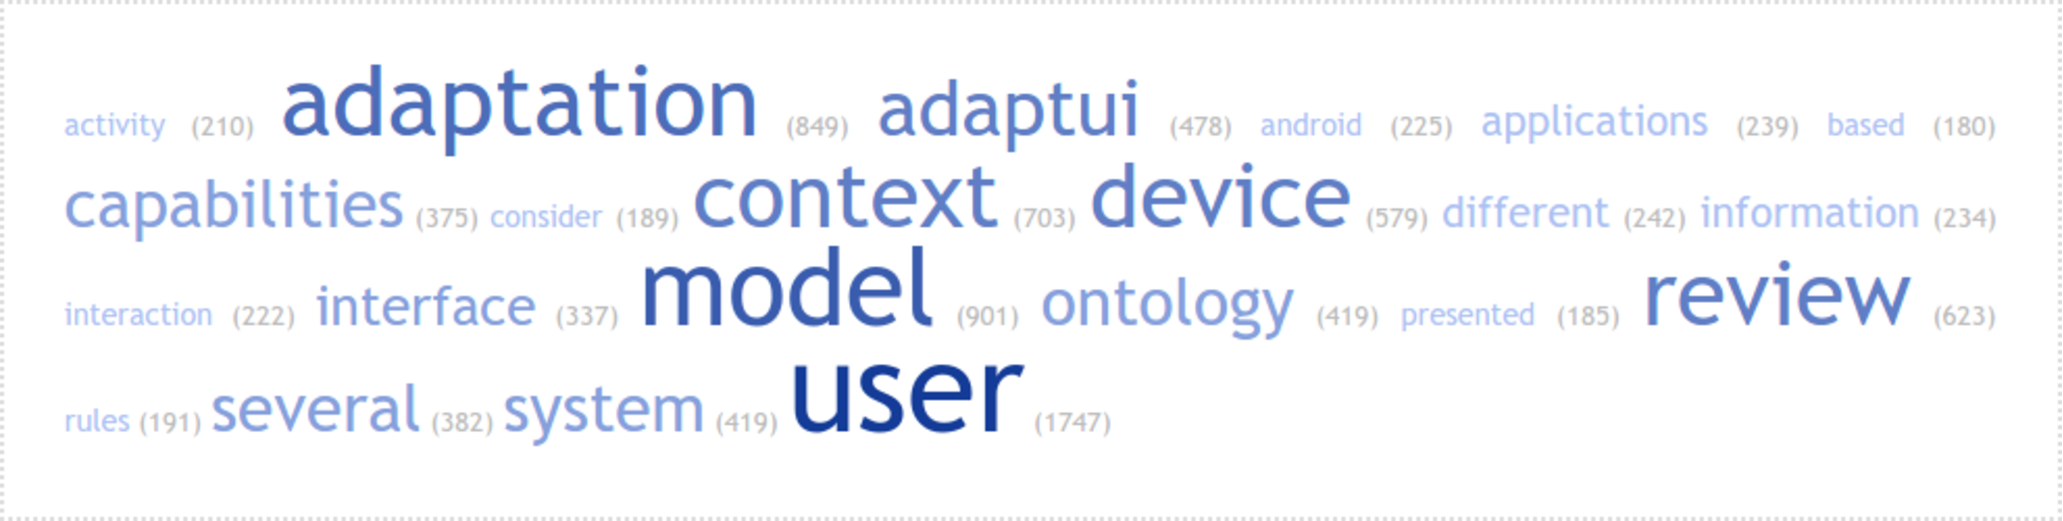
\includegraphics[width=0.70\textwidth]{tagcloud.pdf}
% \caption{AdaptUI's three-layered global architecture.}
\label{fig:tagcloud}
\end{figure}

%\end{footnotesize}
%\end{multicols}


%: --------------------------------------------------------------
%:                  MAIN DOCUMENT SECTION
% --------------------------------------------------------------

% the main text starts here with the introduction, 1st chapter,...
\mainmatter

%\renewcommand{\chaptername}{} % uncomment to print only "1" not "Chapter 1"
\pagestyle{fancy}

% Do not split the following words
\hyphenation{AdaptUI}
\hyphenation{AdaptUIOnt}
\hyphenation{Imhotep}

%: ----------------------- subdocuments ------------------------

% Parts of the thesis are included below. Rename the files as required.
% But take care that the paths match. You can also change the order of appearance by moving the include commands.

\begin{savequote}[50mm]
You take the blue pill, the story ends, you wake up in your bed and believe 
whatever you want to believe. You take the red pill, you stay in Wonderland, 
and I show you how deep the rabbit hole goes.
% We are marching to a land far from home. No one can say who will return.
% I feel the hard fight has begun, no more living on the run.
% I feel a hard fight has begun, I know it's been done.
% Yes, a hard fight has begun.
\qauthor{The Matrix}
\end{savequote}

\chapter{Introduction}
\label{cha:introduction}

% the code below specifies where the figures are stored
\ifpdf
    \graphicspath{{1_introduction/figures/PNG/}{1_introduction/figures/PDF/}{1_introduction/figures/}}
\else
    \graphicspath{{1_introduction/figures/EPS/}{1_introduction/figures/}}
\fi

%------------------------------------------------------------------------- 

Over the years we are witnessing the growth of new and heterogeneous mobile and
smart devices and services with a wider range of possibilities. Faster processors,
larger memories and more accessible sensor capabilities have allowed the community to
develop context-aware applications which, taking into account the user preferences
and the context situation, can be customized for the final user. This usually
results into the same application having different behaviours, aspects and 
available features depending on the specific target user. Besides, the spread 
of intelligent environments provides relevant information about the current 
context of the agents and involved entities. As a consequence, local 
governments and public administrations have discovered the importance of 
working with context data~\citep{caragliu_smart_2009}. Thus, they try to 
improve cities infrastructures and citizens satisfaction.

This situation has brought the appearance of new research domains. This 
dissertation focuses on one of these domains: adaptive user interfaces. 
Adaptive user interfaces arise from the need to cover a wider range of users 
and environment conditions. This area is related to different research domains 
or trends. For instance, universal or inclusive design. Universal design refers 
to a set of guidelines for producing different kind of environments (i.e., 
buildings, software applications and any kind of product) accessible and usable 
to both people with and without disabilities and dependant people (as the 
elderly).

During this dissertation we have studied how each user has his own preferences,
even those who suffer from similar disabilities. We have also found that usual 
market applications and devices are usually unable to guarantee a comfortable 
interaction in many situations for these users. Although several accessibility 
tools are provided (related to smart devices), these users prefer non smart 
devices due to the physical interaction that they provide (as physical touch 
buttons, not touchable screens). This kind of devices are easy to use and the 
feedback that they provide is also easy to understand. Hence, this situation has
revealed a lack of substantial efforts in the adaptive user interfaces domain. 
This makes this group of users suffer from interaction inattention.

Hardware advances have brought haptic displays, high definition, curved 
screens and cameras, accelerometers and different kind of sensors, faster 
connectivity capabilities, and so forth. On the other hand, software development
allow us to use Internet services as we did with a computer. Nevertheless,
this progress does not reflect the current society requirements (including
inclusive design). While these advances keep reaching the ubiquitous future
there are several groups of people that suffer from inattention: the elderly and
people with disabilities. These users have special needs. The elderly usually
have mobility, sight and hearing problems, while the disabled suffer from more
specific and usually severe impairments. There are several accessibility tools
that try to reduce the existing interaction boundaries between disabled users
and devices~\citep{gregor_designing_2002}\citep{burgstahler_designing_2002}.
For example, the Android operating system allows developers to build more accessible 
applications by using custom controls and interaction alternatives (e.g., 
gestures)\footnote{http://developer.android.com/guide/topics/ui/accessibility/index.html}.
Apple's iOS uses zoom, larger text, colours inversions, dictation and voice
control to avoid interaction issues\footnote{https://www.apple.com/accessibility/ios/}.
Regrettably, these tools are too static. For example, they do not take the user
context into account and they do not understand and learn from the users'
experiences. Besides, they are more adaptable than adaptive. Adaptive systems
have the ability to dynamically adapt themselves to the current task and user.
On the other hand, adaptable systems' functionalities are changed with user
intervention~\citep{fischer_user_2001}.

The fact is that user interface adaptation has evolved in the latests 20 years.
From the simplest preferences (e.g., modifying the resolution of a screen or
monitor) to more sophisticated solutions (e.g., smartphones' brightness automatic
controls), the community has attempted to customize applications as far as 
possible. These adaptations have grown in complexity, covering a wider range of 
users, as well as taking into account the current context situation. Therefore, 
context and user modelling have become a real challenge in this domain. This is 
because of the context variability and the set of different capabilities that 
users can have.

However, current mobile devices offer new possibilities due to their 
computational capabilities. Hence, during the following chapters we present a
series of contributions which are grouped together forming AdaptUI, a user 
interface adaptation framework which has a twofold purpose: to reduce the 
usability problems when users interact with their devices, and to encourage 
developers to include adaptive engines in their applications to make them more 
inclusive.

\section{Background}
\label{sec:background}

To clarify the foundations in which this work relies, and to provide a starting 
point for understanding the rest of the thesis, this chapter introduces and 
describes two related and significant research motivations in which this dissertation is based. 
First, introducing our previous experience with \ac{aui} systems; and secondly, 
describing one of the basis that support the work described in this dissertation, 
which deals with the problem of identifying the user's disabilities and needs.

Consequently, Section~\ref{sec:background_imhotep} introduces Imhotep, an \ac{aui}
framework whose benefits and drawbacks have driven the research performed in this 
thesis. Next, in Section~\ref{sec:background_icf} \ac{icf} and the user capabilities 
related to interaction are addressed.

\subsection{Previous Experience with \acp{aui}: The Imhotep Framework}
\label{sec:background_imhotep}

Conceived in 2010, Imhotep~\citep{almeida_imhotep_2011} stands as the result of 
our first approach to \ac{aui} systems. Imhotep is a framework whose main goal
is to ease the development of adaptable and more accessible user interfaces. 
Designed by developers and \textit{for developers}, this framework allows
writing applications in a way in which developers do not have to worry about the 
adaptation of the user interface. The paradigm in which Imhotep is supported 
deals with the definition of a series of preprocessor directives. With these 
directives both the user capabilities and the device characteristics are taken
into account. 

To make the developed applications available to users, they are uploaded to 
a public repository. Thus, users can download them through an application 
download tool which sends to the server the user's and device's profile. Hence, 
the server compiles the best user interface for these profiles.

One of the benefits of Imhotep is the level of expression of the preprocessor
directives. Developers can establish their own variables and rules.
Listing~\ref{lst:imhotep_pseudocode} shows a piece of pseudo-code where the
developer defines new variables.

\inputminted[linenos=true, fontsize=\footnotesize, frame=lines]{java}{5_experiments_and_results/imhotep_pseudocode.txt}
\captionof{listing}{Imhotep pseudo-code defining variables~\citep{imhotep_website}.\label{lst:imhotep_pseudocode}}

These variables, rules and possible values are defined by the developer using a
web based wizard. Furthermore, the concepts, such as \textit{``resolution is 
big''} are created by the system taking into account the information of the mobile
devices (provided by \ac{wurfl}\footnote{http://wurfl.sourceforge.net/}) and pondering it with their 
popularity (with Google Trends\footnote{https://www.google.com/trends/} data).

The results obtained in Imhotep have motivated this dissertation. Moreover, Imhotep
serves as a good metric to evaluate the benefits of AdaptUI (the \ac{aui} platform 
described in this thesis). A more specific review of Imhotep is given in 
Chapter~\ref{cha:evaluation}, in which the Imhotep's architecture is reviewed 
and its performance compared with AdaptUI.


\subsection{User's Capabilities and Interaction}
\label{sec:background_icf}

Researchers have developed and improved several techniques to model users for 
the past 20 years~\citep{petrelli_user_centered_1999}\citep{fink_adaptable_1997}. 
Modelling users implies gathering knowledge of their capabilities, drawbacks 
and limitations. During these first decades there was not any official and 
medical-based study to support user capabilities. Nevertheless, in 2001 
this situation changed. The \ac{wha}, a forum through which the \ac{who} is
governed, published the \ac{icf}\footnote{http://www.who.int/classifications/icf/en/}. 
\ac{icf} is a classification of human functioning and disability. It 
classifies every function state associated with health (e.g., diseases, 
disruptions, injuries and traumas). Its purpose is to identify the low-level 
capabilities relevant to product design in several domains. As was written by 
experts in the area, \ac{icf} is a reference for identifying several user 
capabilities in any interaction process. Its main goals are the following:

\begin{itemize}
  \item To provide a scientific basis to study and understand health and
  health-related states, outcomes and determinants.
  \item To establish a common language for describing health-related states in 
  order to improve communication between different users, such as health care 
  workers, researchers, policy-makers and the public, including people with 
  disabilities.
  \item To permit comparison of data across countries, health care disciplines,
  services and time.
  \item To provide a systematic coding scheme for health information systems.
\end{itemize}

\ac{icf} is organized into two main groups. On the one hand, Part 1 deals with 
\textit{Functioning and Disability}, indicating problems (e.g. impairment, 
activity limitation or participation restriction summarized under the umbrella 
term disability). On the other hand, Part 2 covers \textit{Contextual Factors}. 
This group gathers a list of \textit{Environmental Factors} which have an impact 
on all components of functioning and disability. The most significant function
groups of Part 1 are highlighted below:

\begin{itemize}
  \item \textit{Body functions}, which are the physiological functions of body 
  systems (including psychological functions). These functions encompass:
    \begin{itemize}
      \item Mental functions.
      \item \textit{Sensory functions and pain}.
      \item Voice and speech functions.
      \item \textit{Neuromusculoskeletal and movement-related functions}.
    \end{itemize}
  \item Body structures, as the anatomical parts of the body such as organs, 
  limbs and their components.
  \item Activities and participation. An activity is defined as the execution of 
  a task or action by an individual. Participation is involvement in a life 
  situation.
  \item Environmental factors, which make up the physical, social and attitudinal
  environment in which people live and conduct their lives.
\end{itemize}

In Part 2, \textit{Environmental factors} include:

\begin{itemize}
  \item Products and technology.
  \item \textit{Natural environment and human-made changes to environment.} It 
  encompasses:
  \begin{multicols}{2}
    \begin{itemize}
      \item Physical geography.
      \item Population.
      \item Flora and fauna.
      \item \textit{Climate}.
      \item Natural events.
      \item Human-caused events.
      \item \textit{Light}.
      \item \textit{Time-related changes}.
      \item \textit{Sound}.
      \item \textit{Vibration}.
      \item Air quality.
    \end{itemize}
  \end{multicols}

  \item Support and relationships.
  \item Attitudes.
  \item Services, systems and policies.
\end{itemize}

Two significant terms that this dissertation uses are \textit{impairment} and 
\textit{environmental factors}, defined by \ac{icf} as follows:

\begin{description}
  \item[\Defi{Impairments, by \ac{icf}}] \hfill \\
    \begin{mdframed}[hidealllines=true,backgroundcolor=gray!20]
    \textit{``Impairments are problems in body function or structure such as a 
    significant deviation or loss''.}
    \end{mdframed} 
    
  \item[\Defi{Environmental factors, by \ac{icf}}] \hfill \\
    \begin{mdframed}[hidealllines=true,backgroundcolor=gray!20]
    \textit{``Environmental factors make up the physical, social and attitudinal
    environment in which people live and conduct their lives''.}
    \end{mdframed} 
\end{description}

% First, the \textit{sensory functions} under the \textit{body functions} category of Part 1 are as the reference for adapting the user interface.

% This dissertation considers the function components remarked above. The 
% description of each component is detailed in Table~\ref{tbl:icf}.

\ac{icf} and its considerations, its mentioned and highlighted functions
classification support the motivation for this thesis.

\begin{table}
  \caption{\ac{icf} components considered in this dissertation.}
  \label{tbl:icf}
  \footnotesize
  \centering
  \begin{tabular}{l l l l}
    \hline
    \textbf{Category} 	& \textbf{Component group}& \textbf{Function}& \textbf{Description}\\
    \hline
    Body functions& Seeing and 	 	& Visual acuity	& Seeing functions of sensing from and	\\
    (Part I)	& related		& 		& contour, both binocular and monocular,\\
		& functions		& 		& for both distant and near vision.	\\
		& Hearing and 		& Hearing 	& Sensory functions relating to sensing \\
		& vestibular		& 		& the presence of sounds and discriminating\\
		& functions		& 		& the location, pitch, loudness and quality\\
		& 			&		& of sounds.				\\
		& Neuromusculos- 	& Mobility of 	& Functions of the range and ease of	\\ 
		& keletal and 		& a joint	& movement of a joint.			\\
		& movement-related 	& 		& 					\\
		& functions		&		&					\\
    \hline
    Natural 	& Climate		& Temperature	& Meteorological features and events, such\\
    environment & 			& Precipitation	& as the weather.			\\
    and human-	&			& Wind		& 					\\
    made changes& Natural events	& 		& Geographic and atmospheric changes that\\
    to environment& 			& 		& cause disruption in an individual's 	\\
    (Part II)	& 			& 		& physical environment.			\\
		& Light			& Intensity	& Level or amount of energy being emitted\\
		& 			& 		& by either a natural or an artificial 	\\
		& 			& 		& source of light.			\\
		& Time-related 		& 		& Natural, regular or predictable temporal\\
		& changes		& 		& change.				\\
		& Sound			& Intensity	& Level or volume of auditory phenomenon\\
		& 			& 		& determined by the amount of energy being\\
		& 			& 		& generated.\\
    \hline
  \end{tabular}
\end{table}


% Besides, in the field of adaptive user interfaces


% \ac{icf} provides a multi-perspective approach to the classification of functioning 
% and disability as an \textit{interactive} and \textit{evolutionary} process. It 
% provides the building blocks for users who wish to create models and study 
% different aspects of this process. The interaction of the components remarked by
% \ac{icf} are illustrated in Figure~\ref{fig:icf_interaction}.
% 
% \begin{figure}
% \centering
% 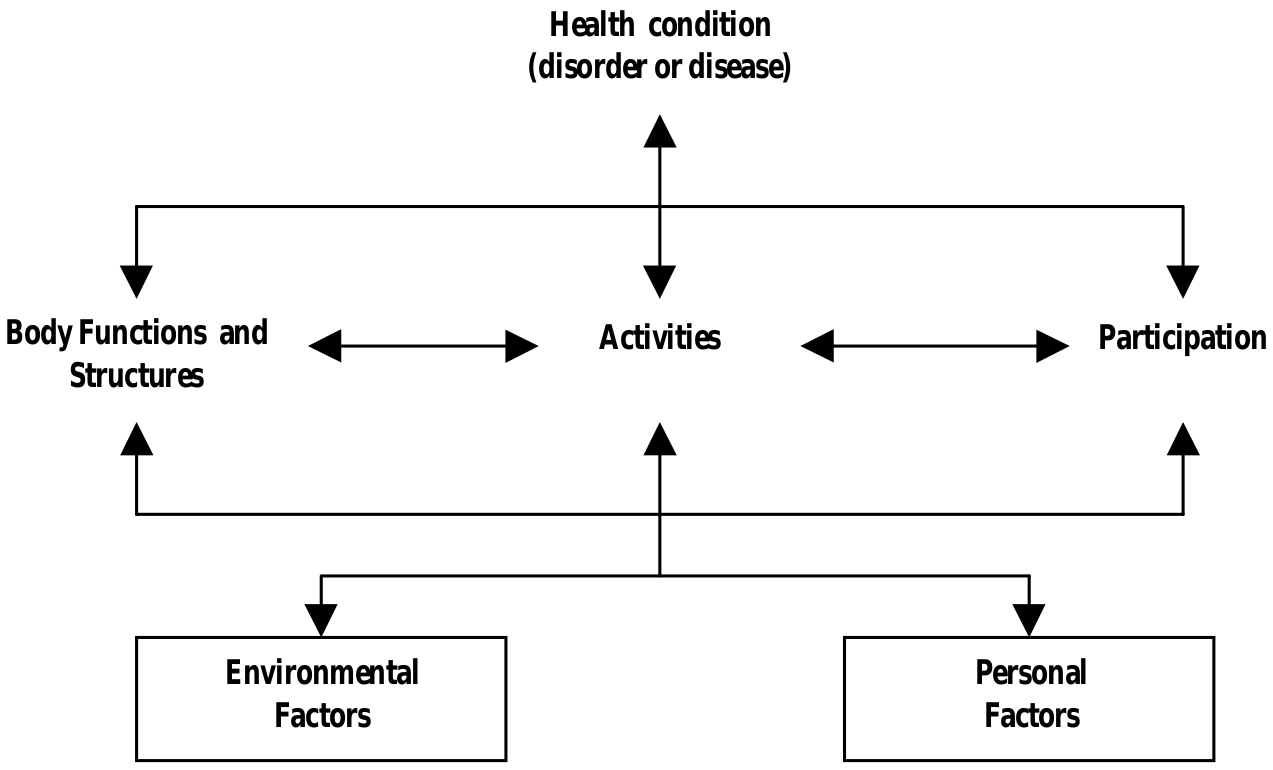
\includegraphics[width=0.75\textwidth]{icf_interaction.png}
% \caption{Interactions between the components of~\ac{icf}.}
% \label{fig:icf_interaction}
% \end{figure}
\section{Motivation}
\label{sec:motivation}

\ac{hci} studies the design of the interaction between computers and users. 
\citet{carlisle1976evaluating} was the first author who wondered about the 
interaction between humans and machines and several possible improvements. 
However, the term \ac{hci} was not used until 1980 by~\citet{card1980keystroke}.

% \ac{hci} is important because poorly designed human-machine interfaces can 
% easily lead to unexpected problems. A classic example of this is the Three Mile 
% Island accident, a nuclear meltdown accident, where the investigations concluded 
% that the design of the human–machine interface was at least partially responsible 
% for the disaster~\citep{nuclear2012backgrounder}. 

\begin{figure}[H]
\centering
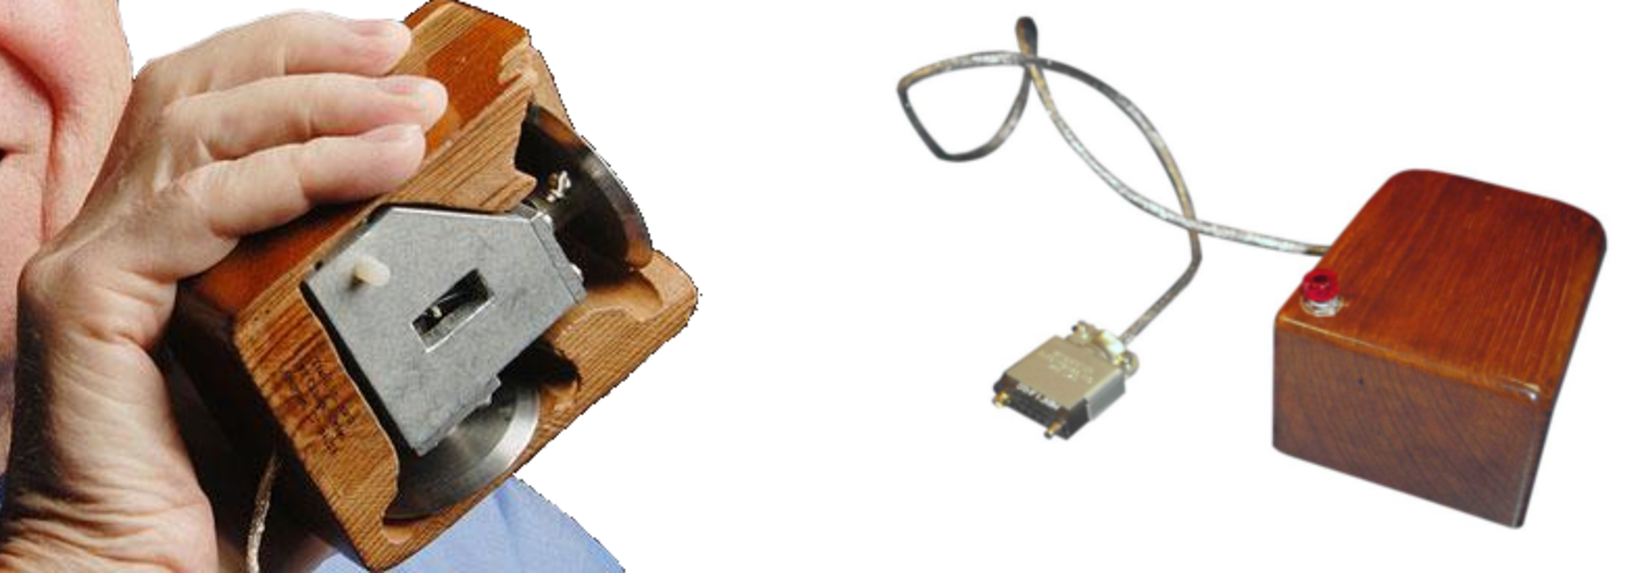
\includegraphics[width=0.70\textwidth]{mouse.pdf}
\caption{First computer mouse by Douglas Engelbart, formed by two wheels 
representing the two axis on the display, and a single button.}
\label{fig:mouse}
\end{figure}

But the concept of \ac{hci} is not relegated to the past evolution of computers 
and industry. It has kept evolving and improving from the invention of the first
computer mouse (see Figure~\ref{fig:mouse}) by Douglas Engelbart during the 
sixties to nowadays interaction advances (see Figure~\ref{fig:google_glasses}\footnote{\url{http://www.google.com/glass/start/}}).
This is thanks to emerging mobile and ubiquitous devices' capabilities, which
have opened new research domains and their power have outstripped the last
decades machines' computational capabilities. Besides, the \textit{mobile device}
concept is almost obsolete, since it has been replaced with what we know as
\textit{smartphones}. Smartphones are feature/mobile phones built over a mobile
operative system and more connectivity and computing capabilities. 

\begin{figure}[H]
\centering
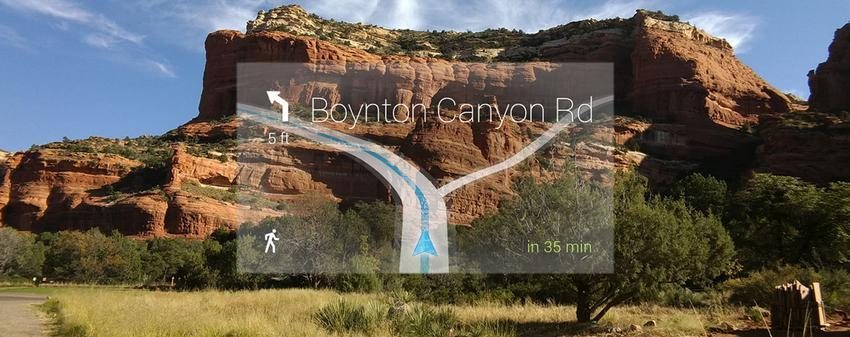
\includegraphics[width=0.70\textwidth]{google_glasses.jpg}
\caption{Google Glasses navigation interface.}
\label{fig:google_glasses}
\end{figure}

Nevertheless, these devices are not just characterized by their power, process,
sensors and connectivity. They also allow developers and designers to include
customization and personalization features. Therefore, they are becoming more
than simple mobile phones. Now they are personal and intimate. They bring us
Internet, email, social networks (e.g., Facebook and Twitter) and so forth. They use
our habits and personal skills to recommend different resources, activities and
even people. And all of this just within reach.

But then, which is the motivation for this dissertation? The answer is found
regarding the target users of the cited adaptation approaches and advances.
To us developing for dependant users and users with disabilities is highly 
needed. Not significant efforts are currently being developed in this area, and 
how important might result having new tools for developers to make their 
applications inclusive. Besides, something that most systems regarding these 
users lack, is the consideration that users with similar disabilities might 
behave in different ways. This is due not only to their capabilities, but also 
due to the way they suffer them, or the influence of other capabilities. For 
example, blindness can be caused by several diseases, injuries, genetic defects 
or poisoning. In addition, people with the same disability might have different 
orientation perception, which might lead into different ways of suffering 
blindness.

Another reason which motivates this dissertation is the fact that nowadays the
share of people aged over 65 represent a 17\% of the current European population. By
the year 2060 this figure is projected to rise to 30\%\footnote{\url{http://ec.europa.eu/economy/finance/articles/structural/reforms/2012-05-15/ageing/report/en.html}}.
As a consequence, and as the European Commission states, \textit{``the \ac{eu} 
would move from having four people of working-age to each person aged over 65 
years to about two people of working-age''}.
The current situation shows that it is still a small group, but with a high 
expected increasing ratio. Nevertheless, this implies that we are still in time 
of accommodating, adapting and overtaking for future economic and demographic 
consequences.

Besides, systems personalization and environment components adaptation have been
demonstrated to benefit both users and service providers~\citep{kobsa_generic_2001}.
However, to achieve a satisfactory adaptation, it is necessary to have several
inputs, for example, a user characteristics model. Hence, the service provider
will be able to apply the corresponding adaptations for the corresponding user.
In addition, current context conditions~\citep{jameson_modelling_2001} and user's
device capabilities are also crucial within this domain. 

On the other hand, being aware of what happens in the user's surroundings is what
researchers called context-awareness. Context-aware applications and systems have
been supported by the community for their significance within user's focused
computing~\citep{schilit_context_aware_1994} \citep{chen_survey_2000}. It is
known that context affects user capabilities. In this dissertation we will see
how these capabilities are somehow influenced by context and how any adaptive
system should react to assure a minimum level of interaction with the user. As a
consequence, we will study each user, context and device capability and we will
present a model which allows to represent the interaction that these entities
may have. 

In spite of the research made by~\citet{kobsa_generic_2001}
and~\citet{fink_review_2000} to get generic user models (more focused on 
Artificial Intelligence) there is a lack of a common, exportable and standard 
models for these environments (adaptive user interface environments) (more 
details provided in Chapter~\ref{cha:state_of_the_art}). Most of the solutions 
presented in Chapter~\ref{cha:state_of_the_art} are strongly domain dependent. 
They rarely represent, for example, the influence of context variables in 
the current domain to perform adaptations. 

Therefore, there is a necessity for a solution that models every entity that
participates in an adaptive user interface environment and a methodology which
permits dynamic adaptations of these entities based on their mutually affecting
capabilities. This methodology will have to take into account several user
reactions with the adapted user interfaces. Consequently, an interaction model
for these environments will be required to evaluate user satisfaction with the
presented user interfaces


\subsection{User's Context Temporary Disabilities}
\label{sec:context_disabilities}

\begin{description}
  \item[\Defi{Product design, by \citet{nelson1977home}}] \hfill \\
  \begin{mdframed}[hidealllines=true,backgroundcolor=gray!20]
  \textit{``Designing an object to be simple and clear takes at least twice as long as 
  the usual way. It requires concentration at the outset on how a clear and 
  simple system would work, followed by the steps required to make it come out 
  that way—steps which are often much harder and more complex than the ordinary 
  ones. It also requires relentless pursuit of that simplicity even when obstacles 
  appear which would seem to stand in the way of that simplicity.'' }
  \end{mdframed}
\end{description}  
  
\citeauthor{nelson1977home} introduced the problems that designing 
a product entails. One of the most significant issues to face during this process 
is the usability. According to the \acs{iso}/\acs{iec} 9126 standard~\citep{isoiec1}, 
quality represents a property of the software product defined in terms of a set 
of interdependent attributes (i.e., usability, security, reliability, performance, 
complexity, readability, reusability) expressed at different levels of detail 
and also taken into account the particular context of software use. At this 
point, the \acs{iso} 9241-11 standard states that usability is the extent to 
which a product can be used by the specified set of users to achieve specified 
goals with effectiveness, efficiency and satisfaction in a specified context of 
use~\citep{iso9241}.

The interaction with devices needs to be satisfactory for the users. The 
\acs{iso}/\acs{iec} 9126-1~\citep{isoiec1} presents and details a two-part model 
for software product quality:

\begin{enumerate}
  \item \textit{Internal and external quality} (see Figure~\ref{fig:ie_q_model}):
  Internal Quality is the totality of attributes of the software product from an
  internal view (e.g., spent resources, analysability). It is measured and
  improved during the code implementation, reviewing and testing. External 
  Quality is the quality when software is running in terms of its behaviour 
  (e.g., number of wrong expected reactions). It is measured and evaluated for 
  software testing in a simulated environment.
  
\begin{figure}[H]
\centering
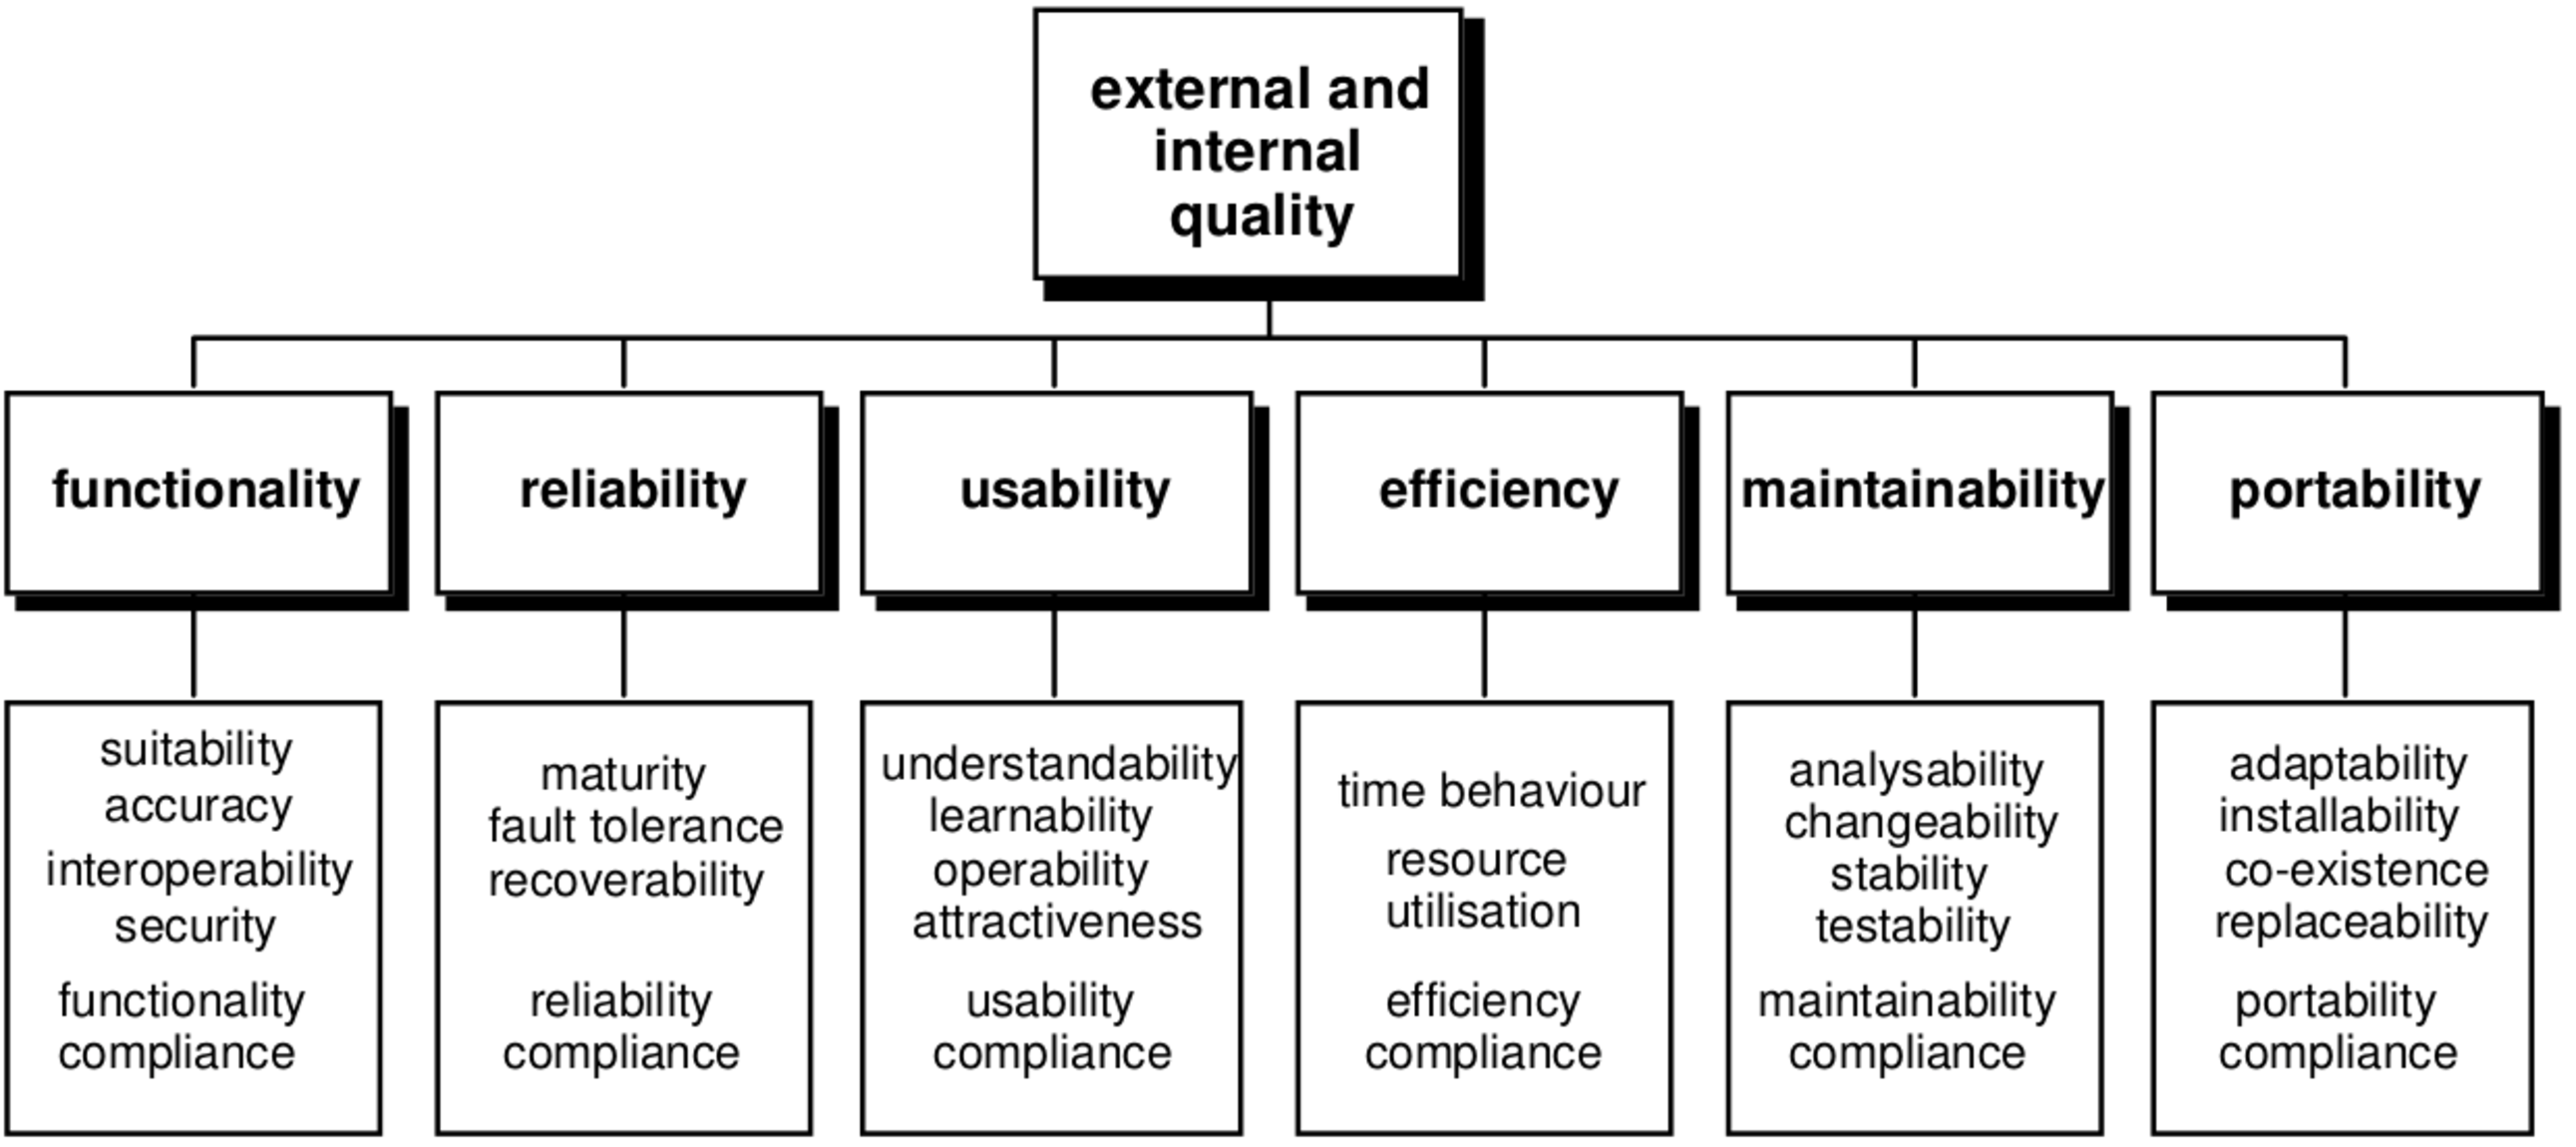
\includegraphics[width=0.75\textwidth]{internal_external_quality_model.pdf}
\caption{Quality model for external and internal quality~\citep{isoiec1}.}
\label{fig:ie_q_model}
\end{figure}
  
  \item \textit{Quality in use} (see Figure~\ref{fig:qu_model}): It is the capability of
  the software product to enable specified users to achieve specified goals with
  effectiveness, productivity, safety and satisfaction in specified contexts of
  use.
\end{enumerate}


\begin{figure}[H]
\centering
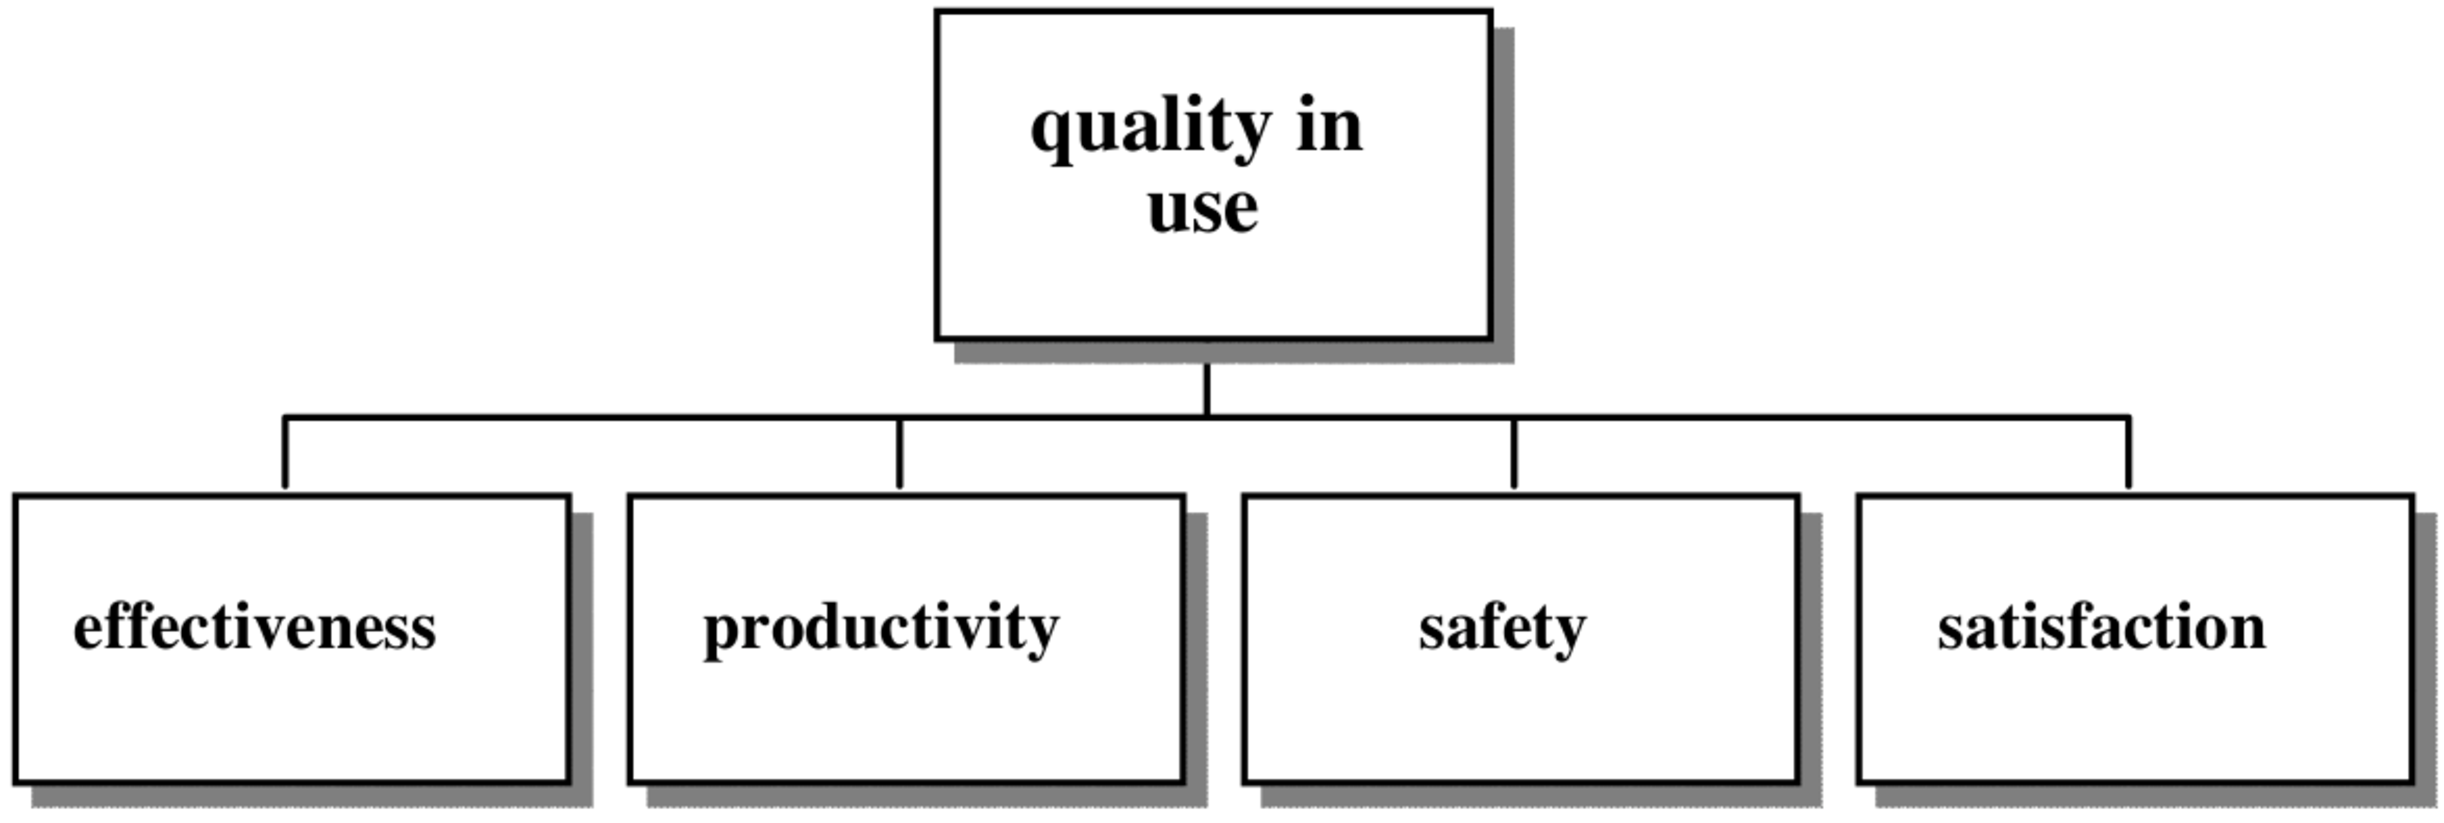
\includegraphics[width=0.5\textwidth]{quality_in_use_model.pdf}
\caption{Quality model for quality in use~\citep{isoiec1}.}
\label{fig:qu_model}
\end{figure}

However, the design process becomes troublesome because of the nature of each
user. Users are very different from each others. They like different things and they
sense and perceive differently. Moreover, they have different capabilities.
Besides, there are several groups which suffer these differences more deeply:
people with disabilities and the elderly. People with disabilities suffer from 
different impairments which are responsible for limiting several capabilities 
in a certain way. For example, users with sight disabilities will suffer from 
interaction problems with their devices if this interaction is based on visual 
stimulus (e.g., using a device display). On the other hand, elderly people 
usually suffer similar interaction troubles due to their ageing. As their 
senses tend to tire their capabilities and interaction levels decrease. Current 
technology trends try to reduce the interaction barriers that elderly suffer 
with nowadays devices. Mobile phones have audio control interaction and screen 
augmentation, \acsp{tv} have zoom and subtitles capabilities, and so on. 
Nevertheless, the elderly are used to use the products they already 
know~\citep{roupa_use_2010}~\citep{elderly_tech}.

% For these groups the designed devices should be [CITA]:
% 
% \begin{itemize}
%   \item \textit{Easy to use}, so the users are able to use them
%   to their own purposes.
%   \item \textit{``Easy to learn''}. This way, the final purpose of the
%   device should be affordable in an acceptable time interval.
%   \item \textit{Easy to recall}, so the users are able to remember how to interact
%   with the device.
% \end{itemize}

Nonetheless, people without disabilities are not exempt of suffering from very
similar situations. There are many conditions in which people without 
disabilities feel like if they had one. Using our smartphone when it is raining 
or with direct sunlight might affect our interaction with the device. These 
situations limit users' capabilities. They are examples of what context is and 
what it is capable of during an interaction process~\citep{dey_understanding_2001}. 
Desktops are less prone to suffer from context conditions (obviously certain 
situations are impossible to avoid, like infrastructure problems). On the other 
hand, mobile devices are predisposed to experience problems due to current context 
situation. 
%[EXPLICAR O APUNTAR A OTRA SECCIÓN DONDE SE EXPLIQUE].

Context is essentially characterized by its capability to change. Besides, as is 
detailed in this dissertation context characteristics can affect several user's 
capabilities. Furthermore, it can change users' capabilities usually
reducing them as they have temporary disabilities. For example, direct sunlight
on a mobile phone screen reduces our sight capability; traffic or crowded streets
reduces our attention and hearing capabilities; several activities (e.g., driving
and cooking) and weather conditions (e.g., raining) affect our attention and
mobility. These are examples of \textit{user's context disabilities}. The first
approximation to this idea was conceived by reviewing the literature. More
specifically, and as is shown in Chapter~\ref{cha:state_of_the_art}, the
thesis by~\citet{heckmann_ubiquitous_2005} presents the following illustration.

\begin{figure}[H]
\centering
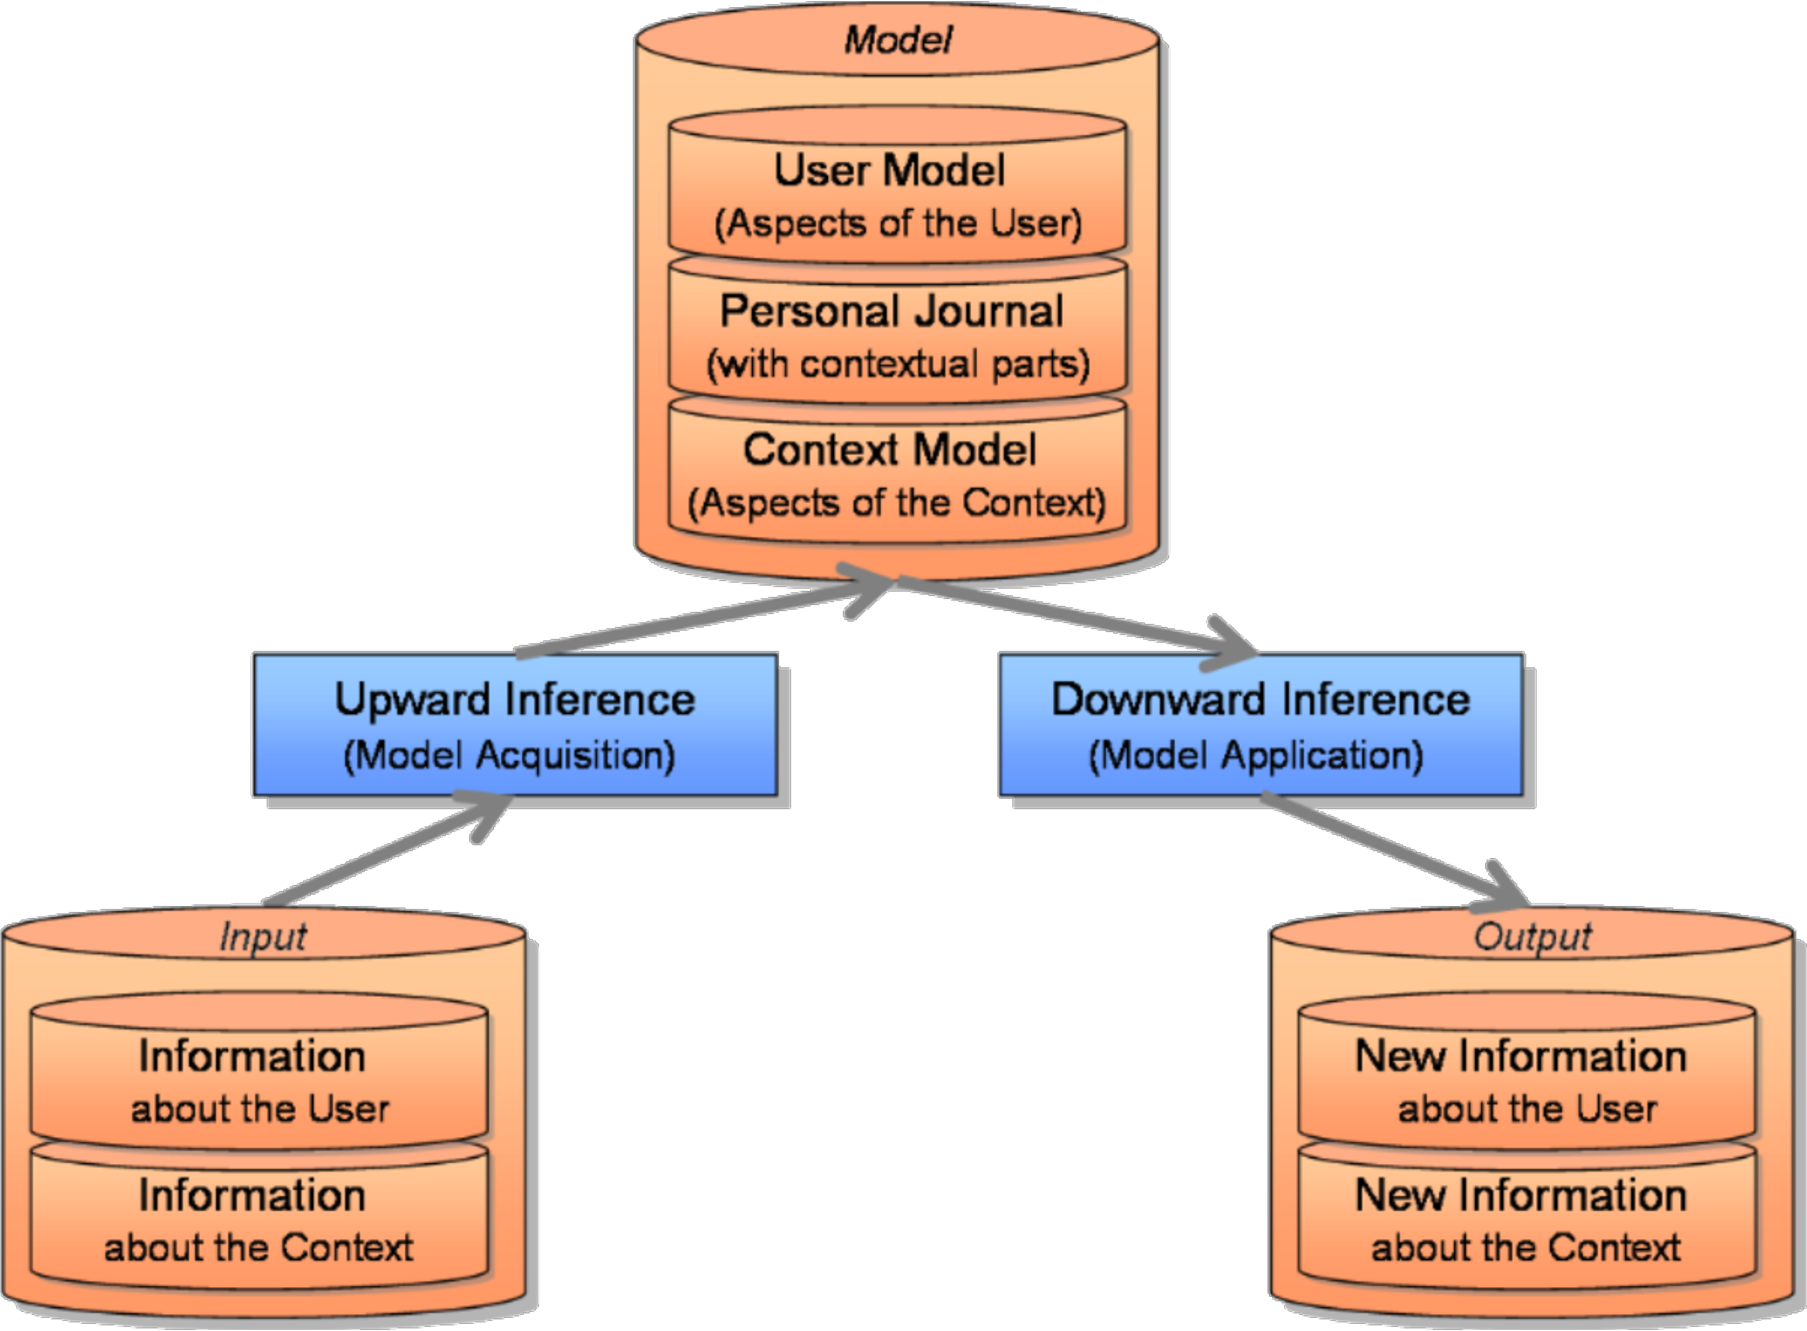
\includegraphics[width=0.6\textwidth]{heckmann.pdf}
\caption{Extended processing schema within context-aware user-adaptive systems, 
derived from~\citep{jameson_modelling_2001} and~\citep{kleinbauer_specter_user_centered_2003},
as appears in~\citep{heckmann_ubiquitous_2005}.}
\label{fig:heckmann}
\end{figure}

Figure~\ref{fig:heckmann} represents a conceptual view of the theory of user 
modelling with integrated context-awareness. The figure presents model acquisition 
and model application information flows. From an \ac{ai} perspective, 
\citeauthor{heckmann_ubiquitous_2005} considers that the input data concerning 
the user and input data concerning the context are processed upward, as an 
inference step. This is what the author calls model acquisition. On the contrary,
the model application works downward, calculating a new hypothesis about the user
or the context. This idea made us understand the user, the context and the device
as evolutionary entities which, in each case, need from specific inference to
result into satisfactory usability with the user interface.

Hence, the main purpose of this dissertation is to dynamically reduce the 
disabilities caused by context on mobile devices by adapting their user interface. 
This will help to maintain certain levels of interaction with the users which 
would be impossible to reach in natural conditions.

\subsection{Definitions}
\label{sec:definitions}

During this dissertation several concepts are often named and referenced. Thus,
in this section these concepts, related to user interface adaptation, the main
discipline tackled by this dissertation, are given. 
% As Chapter~\ref{cha:state_of_the_art} introduces other remarkable
% concepts a complete list of definitions is given in Chapter~\ref{cha:list_of_definitions}.

\begin{description}
  \item[\Defi{User}] \hfill \\
  \begin{mdframed}[hidealllines=true,backgroundcolor=gray!20]
  As the main entity of the AdaptUI ecosystem, a user is understood as an individual
  who has a set of characteristics which define the interaction. These characteristics 
  might represent \textit{capabilities} or \textit{disabilities}. AdaptUI represents 
  a user entity through a semantic model which avoids the explicit representation 
  of such concepts. 
  \end{mdframed}

  \item[\Defi{Context (I), by~\citet{dey_understanding_2001}}] \hfill \\
  \begin{mdframed}[hidealllines=true,backgroundcolor=gray!20]
  \textit{``Contex is any information that can be used to characterize the 
  situation of an entity. An entity is a person, place, or object that is 
  considered relevant to the interaction between a user and an application, 
  including the user and applications themselves''}. Context represents the 
  second main entity in the AdaptUI environment. In this dissertation this 
  definition of context is considered, as we believe that is the most popular 
  definition regarding the literature. As the user and the device, context is 
  semantically represented as a set of characteristics which defines the current 
  situation.
  \end{mdframed}
  
  \item[\Defi{Device}] \hfill \\
  \begin{mdframed}[hidealllines=true,backgroundcolor=gray!20]
  As the third entity included in the studied ecosystem, the device represents 
  the device that the user manipulates within the current context. Devices are
  also understood as a series of characteristics which identify them, including
  both software and hardware related.
  \end{mdframed}
  
  \item[\Defi{Context-aware, by~\citet{schilit_disseminating_1994}}] \hfill \\
  \begin{mdframed}[hidealllines=true,backgroundcolor=gray!20]
  \textit{``Context-aware computing is the ability of mobile user's applications 
  to discover and react to changes in the environment they are situated in.''} 
  In this dissertation several references to context-aware systems are made, 
  specially in Chapter~\ref{cha:state_of_the_art}.
  \end{mdframed}
  
  Distinguishing between adaptable and adaptive user interfaces is significant
  to better understanding the goals of this dissertation\footnote{Although in
  dissertation several adaptable approaches and solutions are analysed (more
  concretely in Chapter~\ref{cha:state_of_the_art}), the final goal of the 
  presented framework is to be adaptive.}. Hence, two definitions remarking the 
  differences between these two concepts are given by~\citeauthor{fischer_user_2001}:
  
  % \mydef{Environment}
  \item[\Defi{Adaptable user interface, by~\citep{fischer_user_2001}}] \hfill \\
  \begin{mdframed}[hidealllines=true,backgroundcolor=gray!20]
  In this dissertation we assume that adaptable user interfaces,
  as~\citet{fischer_user_2001} defines them, are those that change due to the 
  user intervention. In other words, not any user interface component adapts its
  shape or behaviour without the explicit user specification.
  \end{mdframed}

  \item[\Defi{Adaptive user interface, by~\citep{fischer_user_2001}}] \hfill \\
  \begin{mdframed}[hidealllines=true,backgroundcolor=gray!20]
  On the contrary, related to the previous definition, adaptive user interfaces
  have the ability to dynamically adapt themselves to the current task and user,
  not needing the user intervention~\citep{fischer_user_2001}. In the following
  chapters, the reader will easily understand the differences between adaptable 
  and adaptive through several examples and the AdaptUI's architecture detail.
  \end{mdframed}

  \item[\Defi{User disability}] \hfill \\
  \begin{mdframed}[hidealllines=true,backgroundcolor=gray!20]
  This dissertation tries to reduce the possible (or temporary) disabilities 
  that users might suffer when using their devices. To this end, a formal 
  definition of what a disability is, it is needed. As the \ac{icf} document defines, 
  disability \textit{``serves as an umbrella term for impairments, activity 
  limitations or participation restrictions.''}
  \end{mdframed}

  \item[\Defi{Context disabilities}] \hfill \\
  \begin{mdframed}[hidealllines=true,backgroundcolor=gray!20]
  AdaptUI focuses on the interaction of users suffering temporary disabilities 
  caused by the current context conditions. Thus, in this dissertation we 
  introduce the concept of context disabilities. To us, context disabilities 
  are basically temporary disabilities caused by the current context situation, 
  which might limit several user normal abilities or capabilities.
  \end{mdframed}

  \item[\Defi{Physiological capabilities}] \hfill \\
  \begin{mdframed}[hidealllines=true,backgroundcolor=gray!20]
  During the following chapters we refer to physiological capabilities as those 
  capabilities that are included in the \ac{icf} document under the sensory 
  functions classification.
  \end{mdframed}
 
  \item[\Defi{Ontology, by~\citet{gruber_translation_1993}}] \hfill \\
  \begin{mdframed}[hidealllines=true,backgroundcolor=gray!20]
  Ontologies are a \textit{``explicit specification of a conceptualization.''} 
  In other words, it is a formal mechanism to formally represents concepts of a 
  concrete domain.
  \end{mdframed}
  
  % \mydef{Semantics}
  \item[\Defi{Reasoning engine}] \hfill \\
  \begin{mdframed}[hidealllines=true,backgroundcolor=gray!20]
  A reasoning engine (or semantic engine) is a piece of software which is able 
  to infer logical consequences from a set of axioms or assertions. As defined
  in\footnote{\url{https://github.com/owlcs/owlapi/wiki/Reasoners,-OWL-API-Support,-papers-about-the-OWL-API}}, \textit{``a reasoner is a key component for working 
  with \ac{owl} ontologies. In fact, virtually all querying of an \ac{owl} ontology 
  (and its imports closure) should be done using a reasoner. This is because 
  knowledge in an ontology might not be explicit and a reasoner is required to 
  deduce implicit knowledge so that the correct query results are obtained.''}
  \end{mdframed}

  % Inclusive design is defined as follows~\citep{design_2005}: 
  \item[\Defi{Inclusive design}] \hfill \\
  \begin{mdframed}[hidealllines=true,backgroundcolor=gray!20]
  The design of mainstream products and/or services that are accessible to, and
  usable by, people with the widest range of abilities within the widest range
  of situations without the need for special adaptation or design~\citep{design_2005}.
  \end{mdframed}
\end{description}
\section{Hypothesis, Goals and Limitations}
\label{sec:hypothesis}
Based on the current state of Adaptive User Interfaces, the following hypothesis
is developed:
 
\begin{framed}
\textit{User interaction limitations with user interfaces in mobile devices due 
to users' context disabilities are reduced by dynamically adapting the 
corresponding applications' user interfaces through a semantic reasoning process 
which includes: their capabilities as users, the set of characteristics which 
defines the current environment where they actually are, and the devices they 
use. }
\end{framed}

This hypothesis is validated undertaking the following main goal:

\begin{framed}
 To design and implement an adaptive user interface system which runs 100\% in
 the user's device, includes current context situation, and considers several
 possible temporary or enduring user disabilities, using different sets of rules
 which makes the adaptation transparent for the user.
\end{framed}


This objective is achieved through the attainment of the following more specific
steps:

\begin{enumerate}
  \item To study the current state of the art on user interface adaptation 
  systems; user, context and device modelling; and mobile reasoning engines.

  \item To design an ontology which models user capabilities through an abstract
  perspective, context several situations and several device static and non 
  static characteristics. The ontology must consider possible interactions 
  between each entity.

  \item To design a set of rules which allow the interaction between the cited
  entities and the final adaptation of the user interface.

  \item To design and implement a reasoning mobile engine which allows reasoning
  in Android based devices.

  \item To provide an \ac{api} for developers to make available the design of 
  adaptive user interfaces and the edition of existing rules sets, as the 
  knowledge represented through the ontology.

  \item To validate the obtained results both qualitatively and quantitatively.
  
%   \item To model this evolution through a process which will be able
% to dynamically adapt the best and most suitable user interface for each 
% precise 
% context situation.
  
%   \item To demonstrate that it is possible to develop dynamic 
% adaptive applications which are able to reduce the impact of users' 
% disabilities taking into account their own capabilities, the devices' 
% characteristics and those which belong to the current context.
\end{enumerate}


% These general objectives are achieved by fulfilling the following more 
% specific
% steps:
% 
% \begin{itemize}
%   \item To study the current state of the art on adaptive user interfaces and 
% on
%   users, context and device modelling techniques and solutions.
%   
%   \item To design a model, focused on adaptive user interfaces domain, which 
% will allow developers and researchers to model several user capabilities, 
% context situation and device characteristics, their evolution and their 
% influences within the current environment.
%   
%   \item To design an interaction model which will gather several aspects of 
% the user current status and satisfaction with the presented and adapted user 
% interface.
% \end{itemize}


The resulting methodology should also satisfy the following requirements:

\begin{itemize}
  \item The designed model should be descriptive, complete and robust enough to
  be able to represent any possible context-aware situation with the users and
  their devices.
  
  \item The model should represent several user capabilities through an abstract 
  perspective, considering that designers, developers and users might lack of 
  physiological background of capabilities.
  
  \item The designed model should be fully domain independent. Consequently, it
  should be exportable and reusable to external user interface adaptation 
  environments.
  
  \item The model should represent physiological capabilities transparently for
  the user and the developer of the adaptive user interface.
  
  \item The designed and implemented reasoning engine should be compatible with
  Android based devices, allowing the use of rules and reasoning features.
  
  \item The designed \ac{api} should allow developers to design automatically
  adaptive user interfaces and also the modification of the knowledge 
  represented by the ontology.
\end{itemize}

The following features will be considered beyond the scope of this research:

\begin{itemize}
  \item Only capabilities related to visual and hearing are taken into account
  for the dynamic adaptation and the user context disability approach. 
  
  \item No cognitive problems have been faced.
  
  \item In the adaptation process the device battery level is not taken under
  consideration.
\end{itemize}


\section{Thesis Context}
\label{sec:thesis_context}

This thesis has been developed in the context of the research centre Deusto
Institute of Technology, DeustoTech, University of Deusto\footnote{\url{http://www.deustotech.deusto.es/}}.
The work that has made possible the development of this thesis is in the context 
of the following research projects:

\begin{itemize}
  \item \acs{piramide}: Funded by the Spanish Ministry of Industry, Tourism and 
  Trade, the \ac{piramide} project proposes to use user mobile device as a 
  catalizer of the interaction of users with their environment, acting as a 
  sixth sense which aids and assists us facilitating and improving our daily 
  interactions with the objects that surround us in our workplace, home or 
  public administrations.
  
  \item UCADAMI: The User and Context-aware Dynamically Adaptable Mobile 
  Interfaces project, funded by the Industry, Innovation, Commerce and Tourism 
  Department of the Basque Government aimed to create a technological framework
  which allows dynamic user interface adaptation based on the usage and context of
  use of the digital interactive content consumed through mobile devices.
  
  \item \acs{dynui}: The aim of \ac{dynui} is to define an intelligent 
  platform that facilitates the development and deployment of user-environment 
  interfaces adaptable to the users, their interaction devices and their 
  context. These interfaces have to be adapted both at the beginning and 
  during the execution of services taking into account the users' capacities, 
  their interaction devices and the users' and their environment's current 
  context.
 
\end{itemize}







\section{Methodology}
\label{sec:methodology}

Achieving the detailed goals requires the following research strategy:

\begin{enumerate}[label=\alph*)]
  \item To perform an exhaustive review of the state of the art in the areas 
  of user, context and device modelling, semantic reasoning and ontologies.   
  This analysis has been reinforced by attending specialized scientific   
  congresses.
  
  \item Perform a critical evaluation of the existing solutions, analysing 
  their limitations and scope and identifying the corresponding areas where it 
  was possible to make a contribution to the state of the art.
  
  \item To design and develop the different modules of AdaptUI infrastructure, 
  by gradually extending their scope and capabilities.
  
  \item To carry out several experiments and evaluate the performance of the 
  developed modules.
  
  \item Attending congresses to present the achieved contributions with the 
  purpose of receiving the corresponding feedback from the scientific 
  community.
  
  \item Network with experts at conferences and meetings.
  
  \item Update the contributions and redesign the system with the feedback 
  attained from the previous actions.
  
  \item To develop and deploy the final dynamic user interface adaptation 
  infrastructure, which takes into account the user, context and device current 
  characteristics to provide the best suitable user interface.
  
  \item Disseminate the results obtained to the scientific community.
\end{enumerate}

Figure~\ref{fig:methodology} summarizes and illustrated the cited and 
followed methodology.


\begin{figure}[H]
\centering
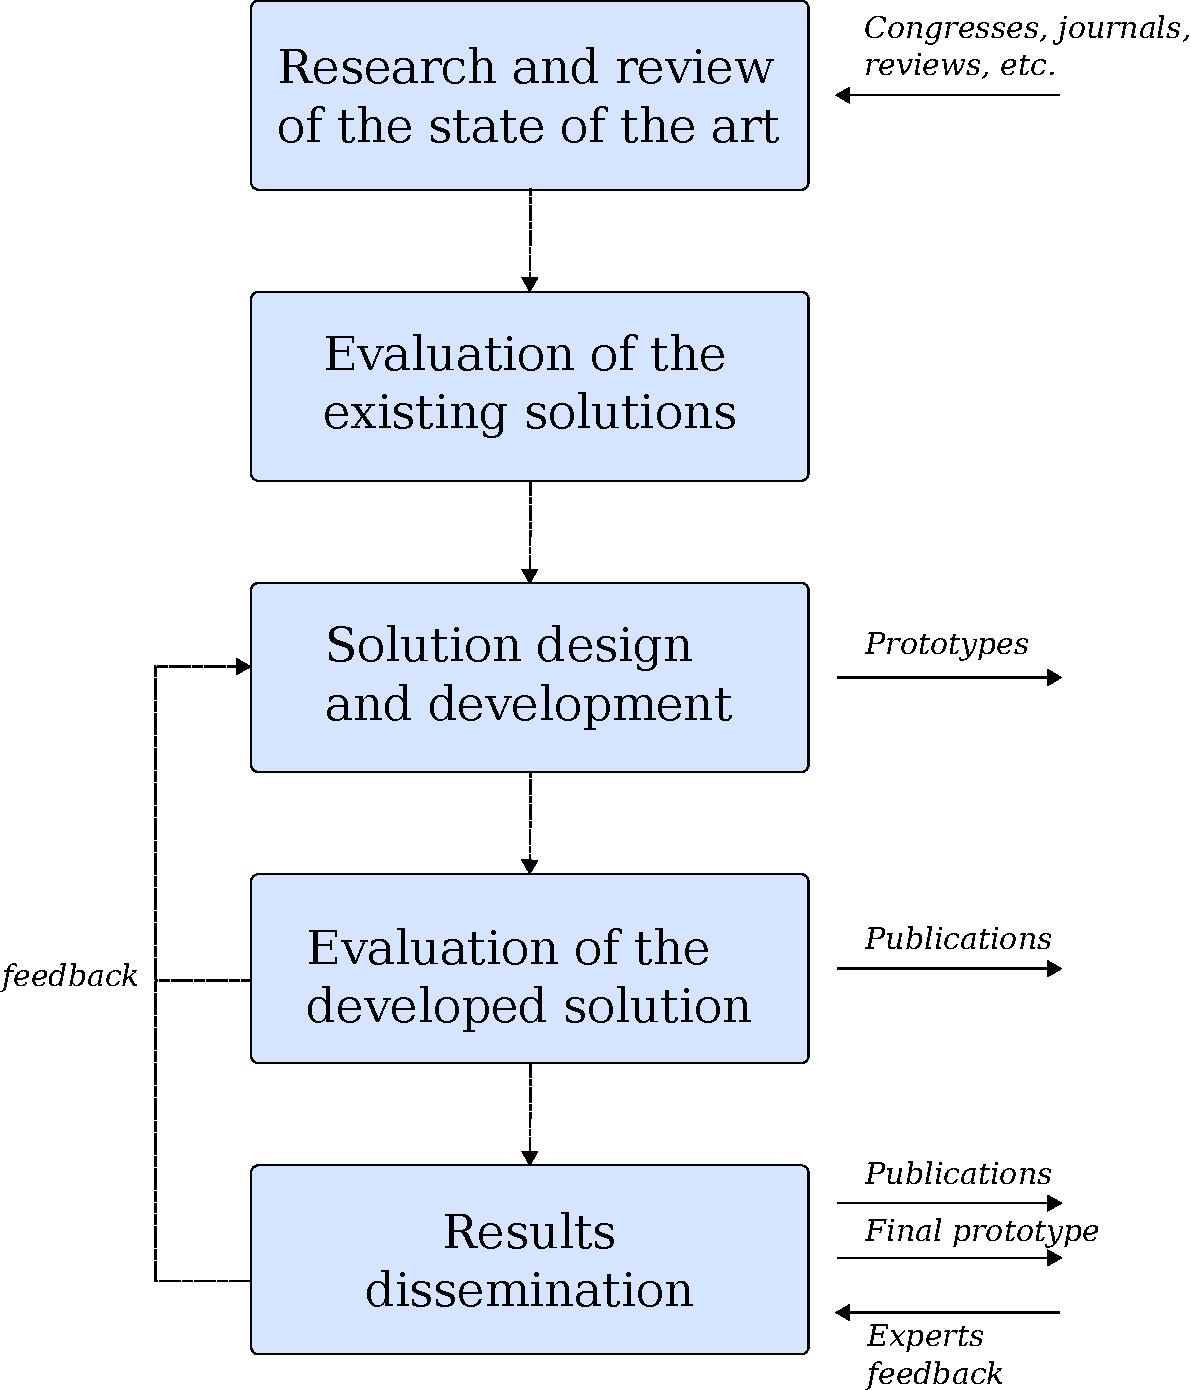
\includegraphics[width=0.60\textwidth]{methodology.pdf}
\caption{Followed research methodology.}
\label{fig:methodology}
\end{figure}

\section{Outline of this Thesis}
\label{sec:outline}

This thesis is presented in 6 chapters (including the current one). As a guide 
to the organization of the remainder of this thesis:

\hspace*{5mm} \textbf{Chapter 1} outlines the motivation, hypothesis, goals and 
limitations of this research. It also describes the followed research 
methodology. \\

\hspace*{5mm} \textbf{Chapter 2} analyses the state of the art regarding user, 
context and device modelling, as well as the different adaptation solutions in 
the last twenty years. \\

\hspace*{5mm} \textbf{Chapter 3} presents AdaptUIOnt: an ontology for 
dynamic user interface adaptation specially designed for this dissertation, 
but also aiming to be used by the scientific community in the user interface 
adaptation domain.\\

\hspace*{5mm} \textbf{Chapter 4} presents the three layered architecture of 
the AdaptUI system, decoupling its modules, their purposes, and main 
characteristics.\\

\hspace*{5mm} \textbf{Chapter 5} outlines and analyses the corresponding
experiments, specially performed to evaluate the whole AdaptUI platform. This
evaluation is divided in two different parts. The first one, regarding only
technical issues of the developed system. The second one, pursuing the 
satisfaction of users.\\

\hspace*{5mm} \textbf{Chapter 6} draws the conclusions of this research work. We 
discuss the achieved goals and analyse the advantages and drawbacks of the 
developed system. Some future lines of research are proposed and the chapter 
ends with some final remarks.\\

% \hspace*{5mm} \textbf{Appendix A} details the classification of the disabilities
% considered for this dissertation. To do this the \ac{icf} document and the
% considerations by \citet{persad_characterising_2007} are detailed.\\

% \hspace*{5mm} \textbf{Appendix B} presents the default included rules in the
% AdaptUIOnt, divided into the corresponding sets of rules depending on their concrete
% goal.\\
% 
% \hspace*{5mm} \textbf{Appendix C} shows the results of the user evaluation
% described in Chapter~\ref{cha:evaluation}.\\


% this file is called up by thesis.tex
% content in this file will be fed into the main document

%: ----------------------- introduction file header -----------------------
\begin{savequote}[50mm]
Looking inside of yourself, you might see someone you don't know. 
Maybe it's just what you need, letting the river in you flow. 
\qauthor{Ronnie James Dio - Caught In The Middle}
%“And upon the top of the pillars was lily work: so was the work of the pillars finished.”
%
% Bible quotes
\end{savequote}


\chapter{State of the Art}
\label{cha:state_of_the_art}

% the code below specifies where the figures are stored
\ifpdf
    \graphicspath{{2_state_of_the_art/figures/PNG/}{2_state_of_the_art/figures/PDF/}{2_state_of_the_art/figures/}}
\else
    \graphicspath{{2_state_of_the_art/figures/EPS/}{2_state_of_the_art/figures/}}
\fi

%------------------------------------------------------------------------- 

This chapter introduces several significant models and techniques related to 
adaptive user interfaces and systems during the past 20 years. Besides, user-oriented,
context-aware and device models and solutions are reviewed. Once the general
domain in which this dissertation lies has been analysed during this chapter,
the specific approaches that are close to this proposal are examined. Thus, 
the way previous proposals have addressed this dissertation's aspects will be 
analysed, highlighting their goodness and weaknesses.  

First, in Section~\ref{sec:adaptation_models} several important adaptation models
are introduced. The performed methodology and modelled parameters are analysed in
detail. Next, Section~\ref{sec:user} focuses its attention in the models
that have been used during the past 20 years for characterizing the user and his/her
capabilities. Section~\ref{sec:context} analyses the most significant
context-aware systems and the way these approaches model the context and its
characteristics. Devices are also one of the main entities that are taken into
account in this dissertation for the adaptation process. Therefore, Section~\ref{sec:devices}
examines several modelling techniques and the devices' capabilities in different
domains.

Besides, a chronological review of the evolution of the presented models will be
depicted in each section.

\section{Adaptation Models}
\label{sec:adaptation_models}
%------------------------------------------------------------------------- 

Before introducing the analysed adaptation models, a terminology review is
given taking into account the differences between adaptable and adaptive
defined by \citeauthor{fischer_user_2001} (see these definitions in 
Section~\ref{sec:definitions}). \\

\citet{fischer_user_2001} defined \textit{adaptive} and \textit{adaptable} 
principles in 2001 through 6 different concepts: definition, knowledge, strengths, weaknesses, required mechanisms, and application domains. 
Table~\ref{tbl:fischer} shows a representation of these concepts.

\begin{table}
 \caption{~\citet{fischer_user_2001} comparison between adaptable and adaptive systems.}
 \label{tbl:fischer}
 \footnotesize
 \centering
\begin{tabular}{l l l}
  \hline
			& \textbf{Adaptive} 			& \textbf{Adaptable}\\
  \hline
	Definition	& Dynamic adaptation by the system  	& User changes (with substantial system	\\
			& itself to current tasks and current 	& support) the functionality of the system\\
			& user.					& ~					\\
	Knowledge	& Contained in the system; projected in & Knowledge is extended.		\\
			& different ways.			& ~					\\ 
	Strengths	& Little (or no) effort by the user; no & User is in control; user knows her/his\\
			& knowledge of the user is special	& task best; system knowledge will fit 	\\
			& required.				& better; success model exists.		\\
	Weaknesses	& User has difficulty developing a 	& Systems become incompatible; user must\\
			& coherent model of the system; loss  	& do substantial work; complexity is 	\\
			& of control; few (if any) success	& increased (user needs to learn the 	\\
			& models exist (except humans).		& adaptation component). 		\\
	Mechanisms	& Models of users, tasks, and dialogs;	& Layered architecture; domain models 	\\
	required	& knowledge base of goals and plans;  	& and domain-orientation; back-talk from\\
			& powerful matching capabilities;  	& the system; design rationale.		\\
			& incremental update of models.		& ~ 					\\
	Application	& Active help systems, critiquing 	& Information retrieval, end-user	\\
	domains		& systems, differential descriptions, 	& modifiability, tailorability, 	\\
			& user interface customization, 	& filtering, design in use.		\\
			& information retrieval.		& ~					\\
  \hline
\end{tabular}
\end{table}

As it is shown in Table~\ref{tbl:fischer}, an adaptive system is able to 
dynamically change due to certain situation. Adaptable systems, however, require 
the user intervention. Current smartphones provide a set of tools to allow users
to adapt several elements of the user interface. For example, font sizes, colour 
combinations, screen magnification and dictation are several adaptable 
functionalities available in such devices~\citep{android_accessibility}~\citep{ios_accessibility},
known as accessibility tools. Figure~\ref{fig:accessibility_ios} shows an example 
of several accessibility tools in iOS.

\begin{figure}
\centering
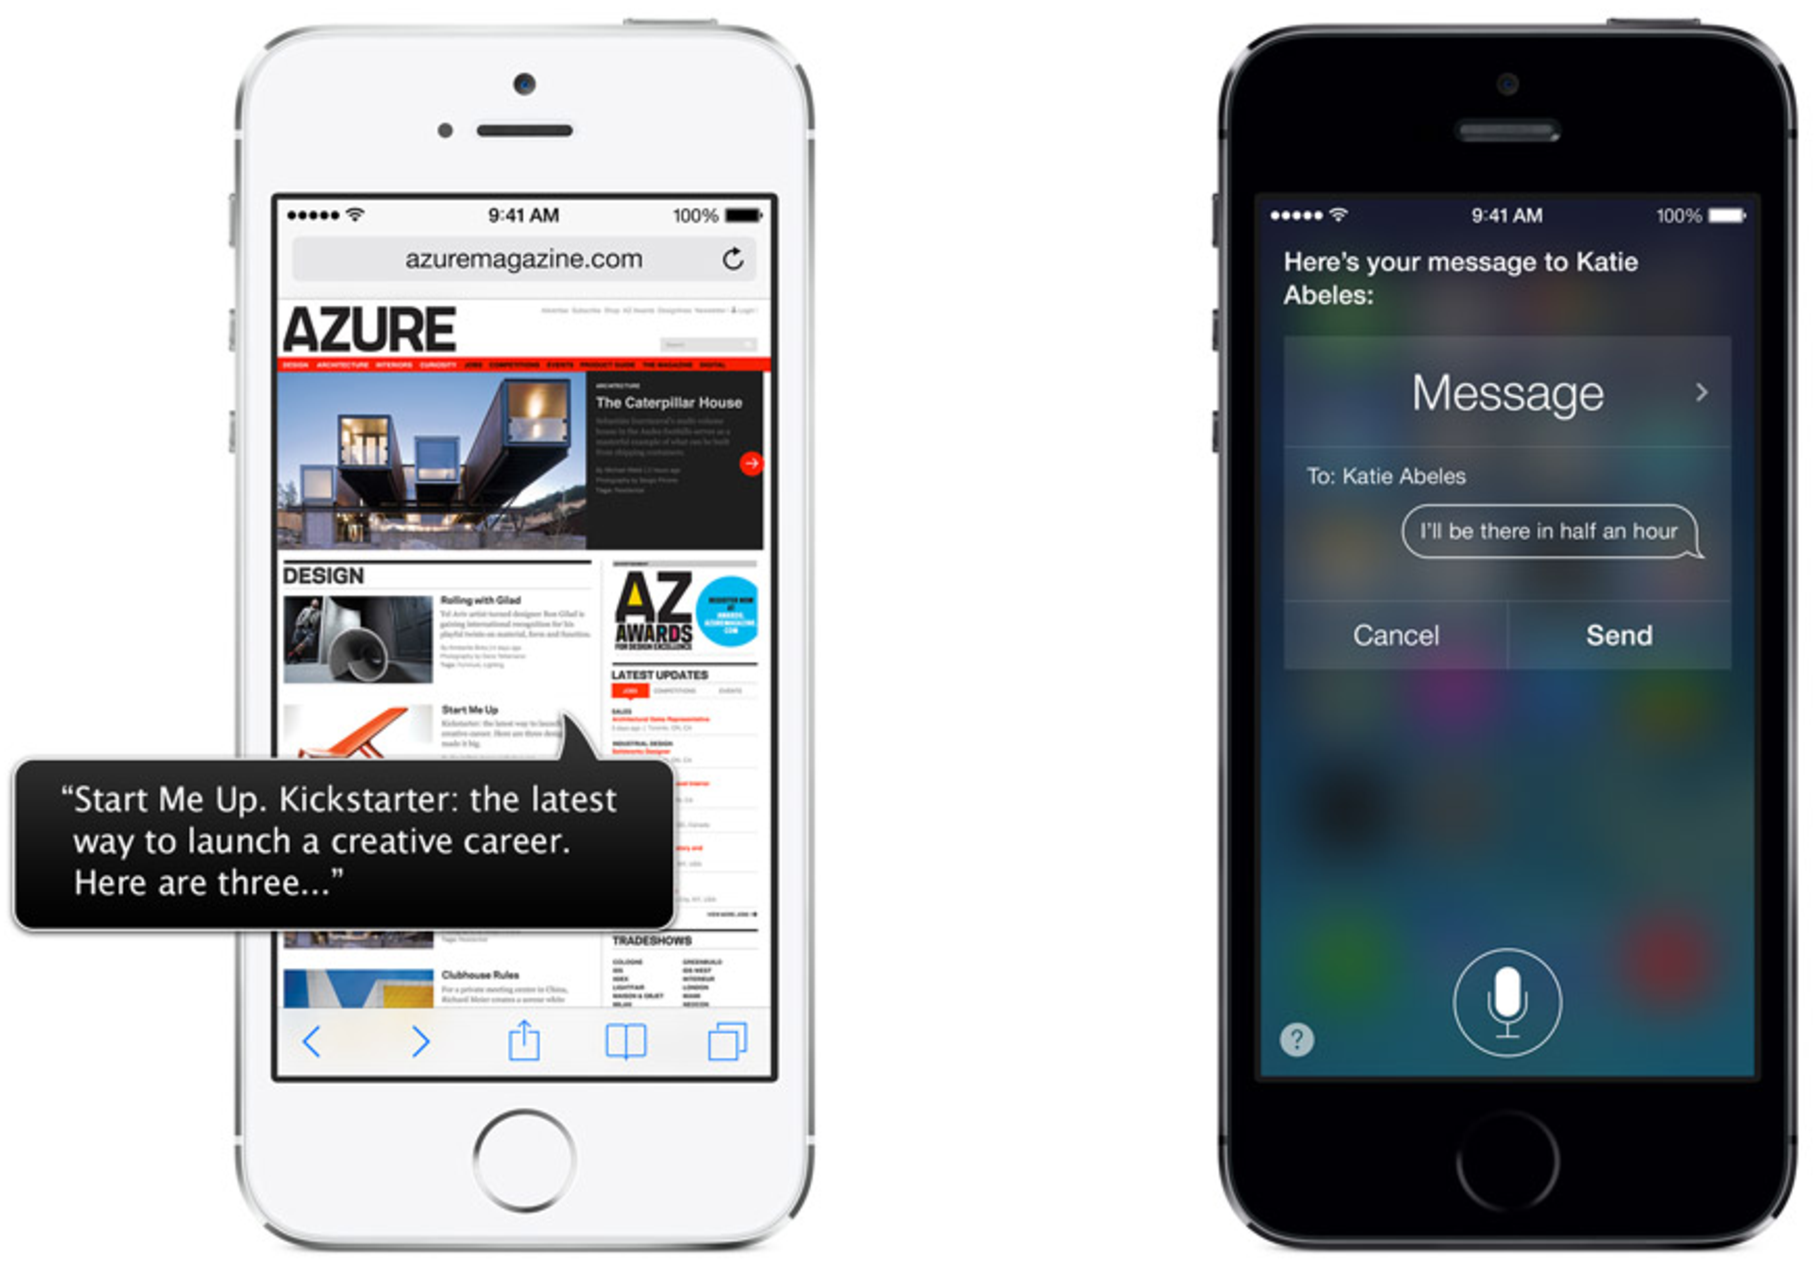
\includegraphics[width=0.7\textwidth]{accessibility_ios.pdf}
\caption{Several iOS accessibility tools~\citep{ios_accessibility}. On the left, 
VoiceOver~\citep{ios_voiceover}. On the right, Siri~\citep{ios_siri}.}
\label{fig:accessibility_ios}
\end{figure}

These accessibility functionalities make the user interfaces \textit{adaptable}
by the users. On the contrary, \textit{adaptive} user interfaces would modify 
the aspect of the shown elements without the user intervention. This means that 
adaptable user interfaces needs the user to change the corresponding adaptable 
characteristic (e.g., the font size) while an adaptive user interface would 
adapt without it.

Thus, once \textit{adaptable} and \textit{adaptive} concepts have been defined,
\textit{adaptivity} and \textit{adaptability} are introduced. \textit{adaptivity}
is related to the fact that a system or a service is able to learn somehow to 
change itself to increase the user satisfaction in the interaction process. 
On the other hand, \textit{adaptability} deals with the property of the system
or service to be customized by the user~\citep{jameson_modelling_2001}.

Now that we have defined what adaptivity means, several significant adaptive 
systems are presented in the following lines.

User interface adaptation has evolved through \ac{hci} history. First, and dealing with
the concept of adaptability (and not adaptivity), user interfaces start to be malleable. 
Colour palettes and screen resolution tools were given to the user. Nowadays, regarding
our portable devices, even automatic brightness control systems are available (dealing
with adaptivity). Since many years, developers have attempted to offer customization
tools to the end user. These tools have grown in complexity, covering a wider range of
functionalities and also users. What is more, a few years ago the context was taken
into account as the set of characteristics that define a situation.

Systems personalization and environment components adaptation has been demonstrated
to benefit both users and service providers~\citep{kobsa_generic_2001}. However, for
achieving a satisfactory adaptation it is necessary to have several inputs, for example,
a user characteristics model. Hence, the service provider will be able to apply the
corresponding adaptations for the corresponding user. Besides, we believe that current
context conditions~\citep{jameson_modelling_2001} and user's device capabilities are also
crucial within this domain. 
% In Section~\ref{sec:interaction_entities} we dig in
% this idea.

\citet{nilsson_model_based_2006} considered that designing user interfaces for
mobile devices tends to be problematic for several reasons (e.g., screen size is
small and interaction mechanisms are very different from a desktop system). Besides,
these devices are usually used in dynamic environments (i.e., variations in the
context). 

In the literature several context based user interface adaptation solutions can 
be found. Before reviewing them, it is necessary to first formally define context.
According to \citet{weerawarana_bean_2001} and \citet{dey_understanding_2001} 
context is defined as any situation that can be used to characterize the situation 
of an entity, taking an entity as a person, a place, or an object that is considered
relevant to the interaction between the user and the application (see
Section~\ref{sec:context}). The definition of \textit{use context} inherits from
the context definition itself as the set of variables values which models the
used device, so as the physical and social environment where the interaction is
being performed.

\citet{calvary_plasticity_2002} stated in 2002 that a user interface is \textit{plastic}
if it is capable to adapt itself taking into account context changes keeping
the usability. They presented a process and a dynamic software mechanism which
supports context variability. This work was supported by the idea that context
changes may provoke the triggering of several reactions under a \textit{prologue-action-epilogue}
paradigm. 
% In addition, to enhance the performance they introduced a
% \textit{historical of contexts}. By selecting pre-known configurations the
% adaptation process resulted faster. This historical database stores several
% context situations and the corresponding computed reactions. Besides, the
% \textit{''Plasticity Threshold"} and \textit{``Context Coverage"} novel concepts
% help to set the boundaries of a still valid user interface~\citep{calvary_supporting_2001}.

Using another paradigm,~\citet{lehtonen_dynamic_2002} detailed a tool to perform
dynamic adaptation on documents based on several user parameters (language,
document type, and so on). The presented approach is based on several \textit{configuration
files} (Product Configuration Files) which describe the current user interface and
store the user preferences. The user interfaces are designed with Bean Markup
Language~\citep{weerawarana_bean_2001} (a language focused on user interfaces)
and Java Beans.

Three \textit{middleware} based solutions are highlighted in the following lines.
\citet{repo_facilitating_2004} introduced in 2004 a model that allows the use 
of Web-based user interfaces (as well as the creation of new ones) that covers 
the environment adaptability requirements and context in the best possible way. 
The main problem is given by the range of devices that users typically employ, 
which have different capabilities and run different platforms. This situation 
causes the need of more flexible applications and devices. Repo identified a lack 
of attention in the initial adaptation process (e.g., when the capabilities of the
mobile device are identified). This approach was based on a \textit{middleware}
architecture, and it was capable of detecting new devices in the current environment
(context changes). It allowed services to query for devices' capabilities through 
a middleware architecture. Once a service identified a certain device, it sent 
the corresponding user interface. 

\citet{nilsson_model_based_2006} introduced a \textit{middleware} solution
which was able to build auto-adaptable systems. In this case, the middleware 
leads the adaptation process dynamically, providing several mechanisms to: 
detect changes in the application context, reason about these changes, and adapt 
to them by a dynamic reconfiguration of the current application. 

Based on the same architecture introduced by~\citet{nilsson_model_based_2006},
\citet{hallsteinsen_self_adaptation_2004} presented a system which was able to 
react to context changes recommending alternative configurations in each case.
The benefit for the user comes from the reasonable adaptation decisions took 
by the middleware, being the developer responsible for describing configuration 
options for important variation points.

\citet{stuerzlinger_user_2006} focused their work on desktop applications
adaptations and on the adaptation, reconfiguration and combination of user
interfaces using a \textit{User Interface Facades} system. Based on the definitions
laid down by~\citet{marmolin_medium_1995}, where differences between superficial
personalization (which allows users to select different options between some
predefined) and deep customization (which allows customizing deeper aspects of
the system) were introduced, authors stated the following criteria for adaptive
interfaces:

\begin{itemize}
  \item Fast, simple, or just-in-time customization: users are able to customize
  their interfaces without advanced planning, whenever they need it, and they will
  be able to do it in a simple way.
  \item Not only big personalization, also local ones (at minor scale).
  \item Deep personalization: users can define new customization rules.
  \item Cross-application personalization: interfaces customization must enable 
  different applications to be combined.
\end{itemize}

A \textit{framework} based approach is presented by~\citet{almeida_imhotep_2011}
in 2011. Imhotep is a framework for user interface adaptation based on inserting
preprocessor primitives within the source code. Thus, at compilation time
different versions of the final application are generated due to the corresponding
user and device parameters. A \ac{wurfl}~\citep{wurfl} database was used for modelling
devices and their capabilities. \ac{wurfl} is a \ac{ddr}, a catalogue of mobile 
device information and a framework for adaptation of mobile user interfaces.
By using it, authors ensure to have the latest devices with their capabilities.
As configuration files, the platform checks both user and device capabilities and
uses them to compile the corresponding solution. This approach has the limitation
of being static. This means that each change in the user capabilities needs a new
compilation of the whole application.

A work in progress by~\citet{evers_achieving_2012} et al. tackles the problem of
the need of user interaction in the adaptation process. Their work, centred in
users, discusses about adaptation versus usability defining different types of
adaptation (i.e., forward and backward) and different user ways of interaction
(i.e., implicit versus explicit). This perspective helps developers to take into
account not only technical characteristics (users models, devices capabilities,
context parameters, adaptation engines and so on) but also some psychology to be 
aware of user mood or stress. In stressful situations users may not be comfortable 
with an adaptation engine which asks questions about the process.

Several ideas of the reviewed works are taken into account for the proposed user 
model in combination with the~\citet{casas_user_2008} research. For instance,
the visual handicap metrics in the sensory layer gives an idea of modelling
not the user disability but the minimum needed configuration for a view component
in the screen. This issue is deeply discussed in Section~\ref{sec:user}.

\subsection{Physical Adaptive systems}
\label{sec:pyshical_adaptive_sistems}

Although it is out of the scope of this dissertation, there is a research
pathway dealing with physical adaptive systems. In Tactus~\citep{tactus}, a
company which aims to redefine devices and user experiences by combining the 
modern and traditional interfaces and on-demand buttons on touch
screens for a tactile experience~\citep{tactus_linkedin}, a novel adaptive
technology has been developed. This technology allow screens to dynamically build
physical buttons into a flat touch screen, depending on the current task. For example,
if the user needs to send an email, the keyboard emerges from the screen
as a physical interface. This interface is supported by the combination of
small fluid channels which are routed throughout the Tactile Layer. This layer
enables fluid to expand the top polymer layer to create the physical buttons (see
Figure~\ref{fig:tactus}).

\begin{figure}[H]
\centering
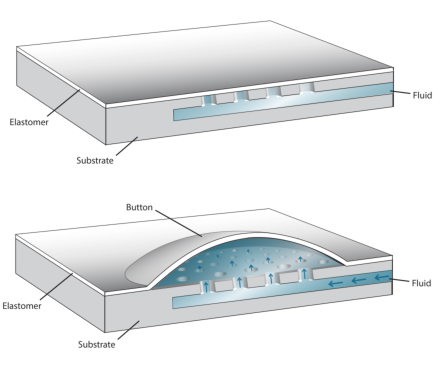
\includegraphics[width=0.55\textwidth]{tactus.pdf}
\caption{Buttons during the flat state (up) and during the raised state (down)~\citep{tactus}.}
\label{fig:tactus}
\end{figure}

Nowadays, this technology might be surprising for the reader. Nevertheless, there
are examples of physical user interfaces adaptation all around us. One of the most
common and spread example is shown in cars. The cars companies deal with adaptivity
for the current driver not just inside the car, but also outside. Some models
adapt the driving wheel in depth and height depending on the driver who unlocks
the door. Displays and controller brightness, even radio volume can be also
adapted considering context light or noise. Even the car lights system adapts
to the road conditions.

Again, these are just a few examples of what adaptation technologies might
be pointing to for the near future.

% ----------------------------------------------------------------------



% this file is called up by thesis.tex
% content in this file will be fed into the main document

%: ----------------------- introduction file header -----------------------
\begin{savequote}[50mm]
Personally, I think it does help, that it makes a beneficial difference, but the scientific literature on the subject is very messy.
\qauthor{Jeanne Petrek}
%“And upon the top of the pillars was lily work: so was the work of the pillars finished.”
%
% Bible quotes
\end{savequote}


\section{User Modelling}
\label{sec:user}

% the code below specifies where the figures are stored
\ifpdf
    \graphicspath{{2_state_of_the_art/figures/PNG/}{2_state_of_the_art/figures/PDF/}{2_state_of_the_art/figures/}}
\else
    \graphicspath{{2_state_of_the_art/figures/EPS/}{2_state_of_the_art/figures/}}
\fi


%------------------------------------------------------------------------- 

\subsection{A Chronological Review of the Evolution of User Models}
\label{sec:chronological_review}

Figure~\ref{fig:user_models} illustrates the chronological evolution and different 
solutions for the last 15 years. During these years different user characteristics 
have been taken into account considering the final purpose of the designed system. 

\vspace{1cm}
\setlength\taskwidth{1.7cm}

\begin{timeline}
  \label{chr:users}
  \Task[1991]{\citet{orwant_doppelgangeruser_1991}}
  \Task[1994]{\citet{brajnik1994shell}, \citet{paiva1994tagus}, \citet{kay1994toolkit}}
  \Task[1999]{\citet{pohl_logic_based_1999}}
  \Task[2001]{\citet{fischer_user_2001}, \citet{kobsa_generic_2001}.}
  \Task[2002]{\citet{gregor_designing_2002}}
  \Task[2003]{\citet{gauch_ontology_based_2003}, \citet{razmerita_ontology_based_2003}}
  \Task[2005]{\citet{hatala_ontology_based_2005}, \citet{pereira_triple_2005}, \citet{heckmann_gumogeneral_2005}}
  \Task[2007]{\citet{persad_characterising_2007}, \citet{golemati_creating_2007}}
  \Task[2008]{\citet{casas_user_2008}}
  \Task[2012]{\citet{evers_achieving_2012}, \citet{skillen2012ontological}}
\end{timeline}
\captionof{figure}{The chronological view of the evolution of remarkable user 
models considered in this dissertation.\label{fig:user_models}}


First user modelling systems started in the late eighties. 
\citet{allen_plan_based_1979},~\citet{cohen_elements_1979}, 
~\citet{perrault_speech_1978}, and \citet{rich_building_1979}\citep{rich_user_1979} 
are examples of researchers whose works inspired next user modelling approaches. 
From there, several authors started collecting different types of information 
about the users and exhibiting, for example, different kinds of adaptations to 
them~\citep{kobsa_generic_2001}.

Before overview the evolution of the user models, a definition of user modelling 
is needed. There are at least two different perspectives which might answer this 
question. One of these is related to \ac{ai}, and it considers user modelling 
as the process through which systems gather information and knowledge about 
users and their individual characteristics. Therefore, a user model is considered 
a source of information about the user of the system which contains several
assumptions about several relevant behaviour or adaptation data. However, in
this thesis the \ac{hci} research perspective is taken, which is defined by
\citet{pohl_logic_based_1999} as follows:

\begin{description}
  \item[\Defi{User Model, by \citet{pohl_logic_based_1999}}] \hfill \\
  \begin{mdframed}[hidealllines=true,backgroundcolor=gray!20]
  \textit{``It refers to an a-priori model of the users of a computer system that the system
  designer has in mind, or to the assumed models that users will probably develop
  of the system and the tasks they can perform using the system''}.
  \end{mdframed}
\end{description}

Nevertheless, this definition and the \ac{ai} perspective coincide in the idea that 
every system must use information about the user to be able to see and react to 
their different problems and needs and improve the system purpose. This section 
analyses the most significant user models in the past 15 years.

\subsection{User models}
\label{sec:user_models}

%sota user models
\subsubsection{1991: Jon Orwan and the Doppelgänger system}
\label{sec:orwant_doppelganger}

Doppelgänger is a user modelling system that performs inferences upon user data
and makes this information available to applications. The system allows users to
modify their models, it makes implicit generalizations about the data (which is
gathered through different channels) and provides an extensible architecture~\citep{orwant_doppelgangeruser_1991}. 

% ``Figure 1 The DOPPELGÄNGER user modelling system gathers data about users from sensors, makes inferences on
% those data, and makes the results available to applications'' cogido de http://www.cs.ucf.edu/~dcm/Teaching/COT4810-Spring2011/Presentations/FrankHines-CheapUserModelingForAdaptiveSystems.pdf

User data is gathered through a continuously operative sensor network which
senses users' everyday activities (see Listing~\ref{lst:orwant_sensor_1}). Hence,
both long-term and short-term information about the user are stored. Sensors are
integrated in users' activities. However, Doppelgänger acknowledges the imperfection
of real world data. Data streams are usually incomplete or erroneous. The main
objective of the Doppelgänger system is to recover from these imperfections through
several learning techniques:

\begin{itemize}
  \item The Beta distribution~\citep{drake_fundamentals_1967}, which is used to
  determine the preference strength, probability of accuracy and the confidence
  of an estimation.
  \item Linear prediction, to predict a possible next event.
  \item Markov models, which represents user's behaviour through several states and
  all possible transitions between them with the corresponding probability.
\end{itemize}


The system maintains an accuracy estimation for each sensor, which helps the
system to decide a confidence metric for the gathered data.

\begin{minted}[linenos=true, fontsize=\footnotesize, frame=lines]{json}
(object orwant location (place 344) (time 779562701) 
(id active-badge))
\end{minted}
\captionof{listing}{Message from a sensor to the server~\citep{orwant_heterogeneous_1994}.\label{lst:orwant_sensor_1}}


The user models are represented in SPONGE, a LISP based data structure manipulated with
C and Pearl programs \citep{orwant_heterogeneous_1994} (see Listing~\ref{lst:orwant_sensor_2}). 
Models are stored as Unix directories consisting of domain submodels and conditional 
submodels. The first one contains information about the user behaviour (i.e., 
location, preferences, and so forth); the second group contains triggering information 
for deciding actions when certain situations are met. Besides, each user model 
is conceptually represented as a point in a high dimensional space in which the 
dimensions are determined by the number of sensors in the network.


% \InsertFig{orwant}{fig:orwant}{Orwant user model \citep{orwant_heterogeneous_1994}}{}{0.70}{}
% 
% \InsertFig{orwant}{fig:orwant_sensors_apps}{The DOPPELGÄNGER user modelling system gathers data about users from sensors, makes inferences on
% those data, and makes the results available to applications. \citep{orwant_for_1996}}{}{0.70}{}

\begin{minted}[linenos=true, fontsize=\footnotesize, frame=lines]{json}
(object orwant primary
  (object biographical_data
    (string_binding "true name" "Jon Orwant")
    (string_binding "e-mail address" orwant@media.mit.edu)
  ...)
  (object control
    (int_binding "doppelganger ID" 4))
...)
\end{minted}
\captionof{listing}{Orwant user model~\citep{orwant_heterogeneous_1994}.\label{lst:orwant_sensor_2}}

% \begin{figure}
% \centering
% \includegraphics[width=0.7\textwidth]{orwant_sensors_apps.pdf}
% \caption{The DOPPELGÄNGER user modelling system gathers data about users from sensors, makes inferences on
% those data, and makes the results available to applications~\citep{orwant_for_1996}.}
% \label{fig:orwant_sensors_apps}
% \end{figure}
% ----------------------------------------------------------------------


\subsubsection{2001: Gerhard Fischer}
\label{sec:fischer_user_2001}

In 2001~\citet{fischer_user_2001} reviews the user models of the past 10 years. 
He describes how using computers in \ac{hci} environments has been always
modelled as a user-computer couple. These elements are modelled as an explicit 
connection which represents the communication between them. New and modern 
interfaces such as windows, menus, pointers, colours, sound and touch screens 
have enlarged this communication line thanks to their capabilities.

Furthermore, in addition to the possibilities of new design approaches,
knowledge-based architectures in \ac{hci} explore the possibility of implicit
communication channel. The required knowledge considers the problem domain,
communication processes and the communication agent. Users are part of the
communication agent group. Fischer defends the idea that there are many types of
users. Besides, their needs change with the experience and through time.
Hence, a simple user classifications (e.g., \textit{novel}, \textit{intermediate}
and \textit{expert}) is not enough to characterize users in complex environments. 
Nevertheless, despite Fischer remarks the significance of each agent, he does 
not establish which agent capabilities are important to face the problem of 
modelling a user.

% \InsertFig{fischer}{fig:fischer}{The human-computer interaction channel 
% \citep{fischer_user_2001}}{}{0.70}{}

\begin{figure}
\centering
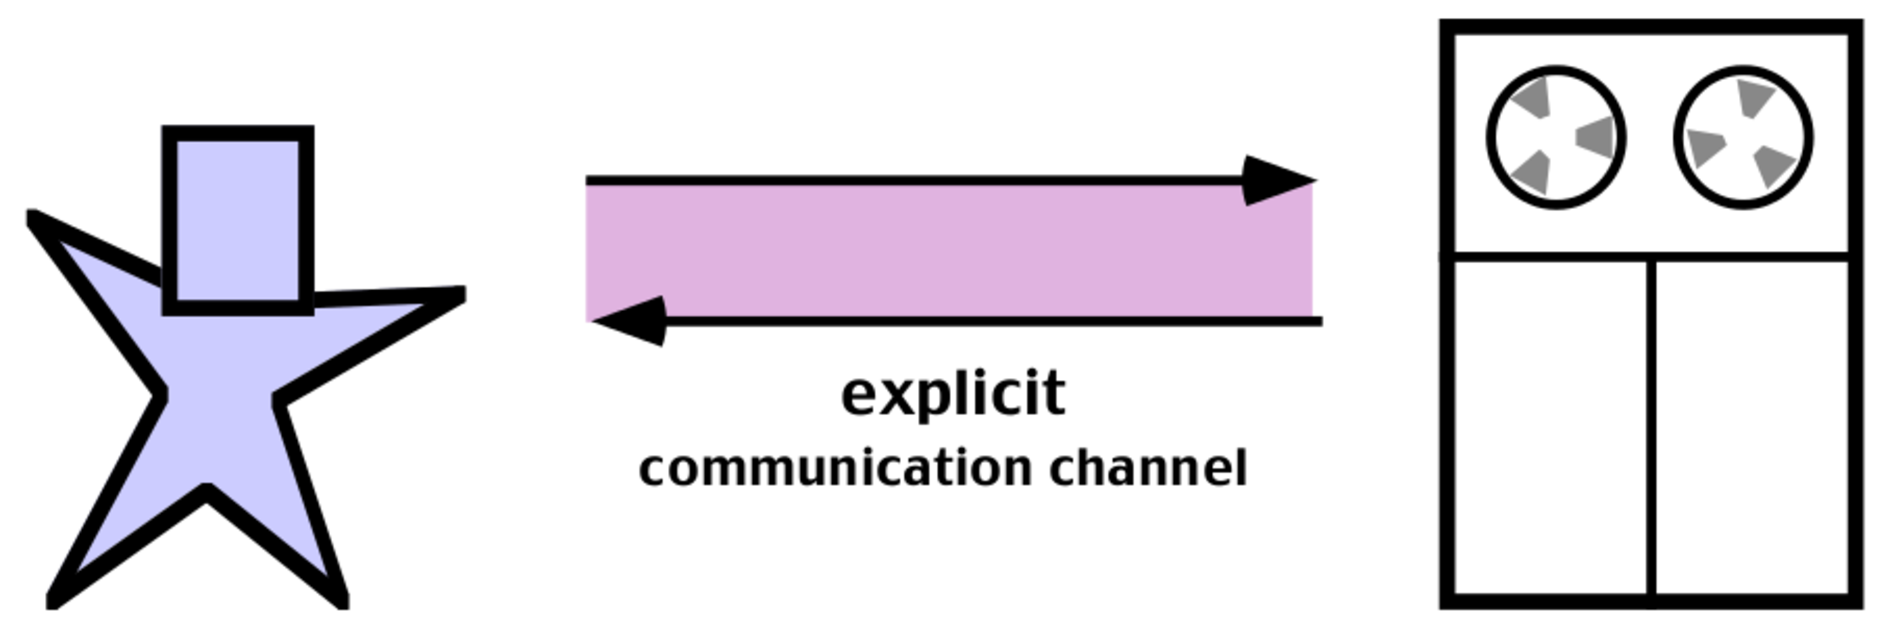
\includegraphics[width=0.50\textwidth]{fischer.pdf}
\caption{The \ac{hci} channel~\citep{fischer_user_2001}.}
\label{fig:fischer}
\end{figure}
\subsubsection{2002: Gregor et al.}
\label{sec:gregor}

%------------------------------------------------------------------------- 
In 2002,~\citet{gregor_designing_2002} focus their approach on a certain groups 
of users: the elderly. A three group classification is presented. In the first 
group there are the fit older people, who do not suffer from any disability. The 
second group is formed by older fragile people who have one or more 
disabilities. Finally, the last group encompasses the older and people with 
disabilities whose capabilities to function depend on other people. In this 
case, the authors identify several user capabilities:

\begin{itemize}
 \item Physical, sensory and cognitive capabilities.
 \item The ability to learn new techniques (cognitive).
 \item Memory problems (cognitive).
 \item The environment can affect several elderly capabilities.
 \item Elderly experience (as a positive fact).
\end{itemize}

On the other hand,~\citet{gregor_designing_2002} consider that, as people grow 
older, their capabilities change. This process encompasses a reduction of 
cognitive, physical and sensory functions depending on the individual. This 
diversity is a significant issue for modelling users and designing computing 
systems.

Figure~\ref{fig:gregor} shows an adaptable user interface which takes into 
account these capabilities. 

% \InsertFig{gregor}{fig:gregor}{Adaptable browsing 
% interface~\citep{gregor_designing_2002}}{}{0.70}{}

\begin{figure}
\centering
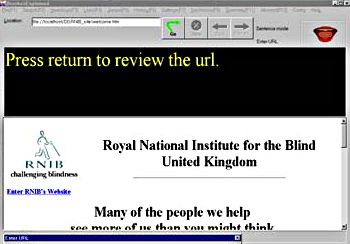
\includegraphics[width=0.70\textwidth]{gregor.png}
\caption{Adaptable browsing 
interface~\citep{gregor_designing_2002}.}
\label{fig:gregor}
\end{figure}

\subsubsection{2003: Gauch et al.}
\label{sec:gauch}

Towards the goal of personalized navigation of online information~\citet{gauch_ontology_based_2003}
provide a user ontology for dynamically modelling the user browsing. The ontology
is formed by several concepts which are weighted indicating the user's perceived
interest in the corresponding concept. These concepts are related with surfing
experience (i.e., the content, length and time spent) on each Web page and
classified into the reference ontology. Hence, the user profile is created 
automatically. This means that the user profile information is collected 
implicitly without user feedback, as the ontology's concepts are automatically 
weighted considering the amount of related information from the user browsing.


% ----------------------------------------------------------------------

\subsubsection{2003: Razmerita et al.: The OntobUM Ontology}
\label{sec:razmerita2003ontology}

Focused in the context of \ac{kms}~\citet{razmerita_ontology_based_2003} present
OntobUM, a generic ontology-based architecture for user modelling. The model is 
generated through two different ways:

\begin{itemize}
  \item Explicitly, using a user profile editor. Thus, the user has to 
  provide some information.
  \item Implicitly, information maintained by several intelligent services 
  which maintain and update the information about the user considering the 
  user's behaviour with the services and provide adapted services based on 
  user's preferences.
\end{itemize}

The architecture of the presented ontology is composed of the following ontologies:

\begin{itemize}
  \item The User Ontology, which structures the different characteristics and 
  preferences of the user.
  \item The Domain Ontology, which defines several concepts about the domain.
  \item The Log Ontology, which manages the semantics of the interaction 
  between the user and the whole system.
\end{itemize}

Authors identify several users' characteristics that are relevant for a \ac{kms} 
under the Behaviour concept. Nevertheless, most of the user ontology is 
generic and it is available to be used in other application domains. 

%Dynamic user modeling? Atención al proceso de captura de datos implícita.

\subsubsection{2005: Hatala and Wakary and the Ec(h)o system}
\label{sec:hatala}

Ec(h)o is an ontology-based augmented audio reality system for museums which 
aims to maintain rich and adaptive output information. The main purpose of this 
work is to address the problem of supporting experience design and functionality 
related to museum visits through user models combined with augmented reality 
and tangible user interface system.~\citet{hatala_ontology_based_2005} find
several challenges for capturing rich context information. For the presented 
museum scenario, social, cultural, historical and psychological factors are 
significant for the user experience. In this field, the argumentation made by
is remarked as relevant. \citeauthor{dourish_what_2004} states that activities 
and context are directly and dynamically linked \citet{dourish_what_2004}\citep{dourish_where_2004}.
This concept is called \textit{embodied interaction}.

The core of the ec(h)o's reasoning module is a dynamically updated user model
\citep{wahlster1989user}. The ruled-based model changes as the user moves 
through the museum and selects several audio objects. This models enables 
developers to consider which inputs influence user interests. In the ec(h)o 
system there are two ways of updating the model: the user movement and a 
selection of an audio object. These actions have different effects on the model 
of the user interests (i.e., influence of initial interest selection, of object 
selection on user interest and of location change). 

As it occurs with recommender systems, user's interest are vital for the concept
ontology. These concepts are weighted in the ontology as concepts which represent
the user's likes within the environment. Besides, an interaction history is 
maintained recording the way the user interacts with the museum. In addition to 
these characteristics the user type is also considered. Hence, the system is 
allowed to characterize the user experience with the environment. It classifies 
users into three different categories:

\begin{itemize}
  \item The \textit{avaricious} visitor, who wants to see as much as possible
  in a sequentially way.
  \item The \textit{selective} visitor, who is more selective with the concepts 
  he/she is interested in.
  \item The \textit{busy} visitor, who prefers to not spend much time and get a 
  general vision of the exhibition.
\end{itemize}

\subsubsection{2005: Fernando Pereira}
\label{sec:pereira}

Within a video adaptation and quality of experience evaluation scenario,
~\citet{pereira_triple_2005} studies a user characterization through three
different dimensions: sensory, perceptual and emotional. First of all,
\citeauthor{pereira_triple_2005} establishes the difference between sensations 
and perceptions as follows:

\begin{itemize}
  \item \textit{Sensations} are monomodal, more low-level, physical and less 
  related to the real world composition than perceptions. They regard the simple 
  conscious experience for the corresponding physical stimulus (e.g., light 
  variation and eyes reaction to this change). They are related to the first 
  contact between a human and the surrounding environment.
  
  \item \textit{Perceptions} are multimodal, and they are part of the cognition 
  process (knowing and learning) and regard the conscious experience and 
  identification of objects.
\end{itemize}

On the other hand, emotions are considered as central in a communication and 
entertainment process. Therefore, \citeauthor{pereira_triple_2005} proposes a 
triple layered \ac{spe} user model for the evaluation of the quality of 
experience in the consumption of multimedia content.





\subsubsection{2007: Heckmann et al.}
\label{sec:heckmann}

A different approach is implemented by~\citet{heckmann_gumogeneral_2005}.
Divided into four main groups (emotional state, personality, characteristics and
physiological state), the authors present the \acf{gumo}, an ontology model to 
characterize users capabilities within adaptive environments. A significant 
user aspect that is taken into account in this work is the stress. In the 
adaptive interfaces domain it is needed to pay special attention to the 
consequences of each adaptation. But the stress is not only determined  by this 
process. It is also derived from several user experiences, as the current 
context state (e.g. traffic, noise, surrounding people, and so 
forth~\citep{babisch_noise_stress_2002}). Figure~\ref{fig:heckmann_model} illustrates
the model presented by~\citeauthor{heckmann_gumogeneral_2005}.

% \InsertFig{heckmann_model}{fig:heckmann_model}{Several user model property
% dimensions~\citep{heckmann_gumogeneral_2005}}{}{0.70}{}

\begin{figure}
\centering
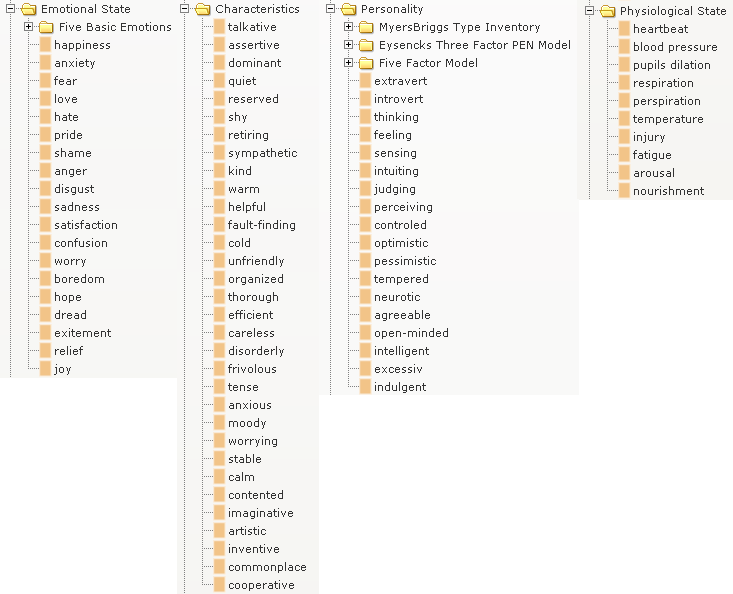
\includegraphics[width=0.70\textwidth]{heckmann_model.png}
\caption{Several user model property
dimensions~\citep{heckmann_gumogeneral_2005}.}
\label{fig:heckmann_model}
\end{figure}

% ----------------------------------------------------------------------

\subsubsection{2007: Persad et al.}
\label{sec:persad}

\citet{persad_cognitive_2007}\citep{persad_characterising_2007} relate user
capabilities and product demands as a tool to evaluate the product design (see Section~\ref{sec:motivation}).
\citeauthor{persad_characterising_2007} remark four main components to consider 
when dealing with interaction between people and technology: the user, the 
product, the environment or context, and the set of activities or tasks 
that define the interaction. The authors try to assess an adaptation degree 
between users and the designed products using different compatibility measures. 
These measures can be assessed on different levels of human capabilities, 
including sensory, cognitive and motor. The concepts of user capability and 
product demand provide a useful framework for analysing the user-device 
compatibility. The product demand levels are considered multidimensional and 
they are set by the interface attributes of the product itself. For example, 
a product's text display will be designed with a certain text size, font, and 
colour contrast. The combination of these attributes define the visual demand 
level within the user visual capabilities. Similarly, other combinations of 
product attributes command several cognitive and motor demands. 

\citeauthor{persad_cognitive_2007} also reviewed functional classifications 
and experimental studies to identify the most relevant low-level skills for 
designing products within the cognitive, motor and sensory domain. This is 
highly related to the \ac{icf} functions described in Section~\ref{sec:background_icf}.

\paragraph*{Sensory capabilities}
\subparagraph*{Visual capabilities:} Several sensory capabilities are known to 
deteriorate with ageing~\citep{persad_exploring_2006}. Thus, 
\citeauthor{persad_exploring_2006} state that the following functions seem to 
account for most of visual disability:

\begin{itemize}
  \item Visual acuity.
  \item Contrast sensitivity.
  \item Colour perception.
  \item Useful field of view.
  \item Stereopsis.
\end{itemize}


\subparagraph*{Hearing capabilities:} Loss of hearing capabilities may directly 
affect the speech interaction with the device. The main low-level hearing 
functions to guarantee the interaction are the following:

\begin{itemize}
  \item Pure tone detection thresholds.
  \item Speech detection and recognition discrimination thresholds.
  \item Sound localization.
\end{itemize}

% \subparagraph*{Environmental effects}
% The level of illumination, noise, weather, etc. are several environment features 
% which might affect user capabilities.

\paragraph*{Cognitive capabilities}
The product's user interface must be usable and accessible enough to guarantee 
that users easily understand the interaction. The following capabilities are 
related to the human cognitive domain:

\begin{itemize}
 \item Working memory performance.
 \item Long term memory.
 \item Mental models, planning and problem solving.
 \item Language and communication capabilities.
\end{itemize}

\paragraph*{Motor capabilities}
\subparagraph*{Upper limb capabilities:}
There are many conditions that affect manipulating a product (e.g., arthritis, 
stroke, multiple sclerosis, head injury, cerebral palsy and missing or damaged 
limbs). These problems directly reduce grasp forces, range of motion and fatigue 
thresholds~\cite{persad_characterising_2007}.

The following areas are highlighted within motor capabilities:
\begin{itemize}
  \item Reach ranges for each arm.
  \item Grasping, dexterity and force exertion.
  \item Two handed actions and coordination.
\end{itemize}

\subparagraph*{Gross body movement capabilities:}
Usually products require certain user mobility degree. 

\bigskip

Besides, \citeauthor{persad_characterising_2007} provide six general categories 
for product features and their interface classification. For this classification 
their toaster case study is considered, \textit{``which is used to demonstrate 
the capability-demand interaction''} (see Table~\ref{tbl:persad_product_interface}).

\begin{table}
  \caption{Product interface classification by~\citet{persad_characterising_2007}.}
  \label{tbl:persad_product_interface}
\footnotesize
\centering
    \begin{tabular}{l l}
    \hline
    \textbf{Feature type} 	& \textbf{Examples} \\
    \hline
    Product chassis 		& Handles, gripping surface. 		\\
    Displays and indicators 	& Visual and auditory displays. 	\\
    Controls and control groups & Discrete controls (button, switch) 	\\
				& and continuous controls (slider,  	\\
				& knob, thumb, wheel, dial, joystick).	\\
				& Control groups \textit{Keypad}. 	\\
    Material/media input 	& Slots (toaster slots), powered and 	\\
    and output			& un-powered bays and trays, doors, 	\\
				& lids and covers.			\\
    Connectors for energy and data & Power and data connectors 		\\
    Software interfaces 	& Navigation menus and \ac{gui} objects. \\
    \hline
  \end{tabular}
\end{table}



\subsubsection{2007: Golemati et al.}
\label{sec:golemati2007creating}

\citet{golemati_creating_2007} present an ontology which considering past 
literature solutions aims to reduce the intrinsic problems of user modelling: 
ad-hoc modelling processes, the required amount of work to model users and the 
possibility of errors by omitting several user's characteristics. To this end,
the authors present an extensible, comprehensive and general ontology whose design
is addressed through a top-down approach by firstly collecting static information
about the user. Next, the ontology designers analyse the semantics of the profile
models and suggest concepts that would adequately model them. It is remarkable
that this work is focused on static user characteristics, although they consider 
the possibility of incorporating dynamic and temporal characteristics.

%Muy importante que modela características. Esto va directo a la parte de discussion de los modelos de usuario





\subsubsection{2008: Casas et al.}
\label{sec:casas}

Another approach is the one presented by~\citet{casas_user_2008}. In this case 
the authors work under the \textit{Persona} concept which is introduced to 
distinguish different user groups within an adaptive user interfaces domain. 
Originally this concept was introduced by \citeauthor{cooper_inmates_2004} in 
1999 by the following definition:

\newpage

\begin{description}
  \item[\Defi{Personas, by \citet{cooper_inmates_2004}}] \hfill \\
  \begin{mdframed}[hidealllines=true,backgroundcolor=gray!20]
  \textit{``Personas are not real people, but they represent them through a design 
  process. They are hypothetical archetypes of real users''}. 
  \end{mdframed}
\end{description}

\citeauthor{casas_user_2008} distinguish between two categories of people:

\begin{itemize}
 \item \textit{Primary}: those who represent the main group and use primary 
 interfaces. 
 \item \textit{Secondary}: those who can use primary interfaces, but with 
 several extra needs.
\end{itemize}

By assigning random values to several characteristics (e.g., age, education,
profession, family conditions, disabilities and technological experience) 
authors are capable of covering a wide range of potential users. However, the 
most significant contribution is that, instead of being focused on users 
capabilities, they consider users needs. To that end they build a user 
profile supported by four main bases: 

\begin{itemize}
 \item The user level, which indicates the ability of the user to face the 
 system.
 \item Interface, for the interaction mechanism to be used by the user.
 \item Audio, to indicate the audio volume levels.
 \item Display, which includes usual display controls (contrast, colours, 
 brightness and so on).
\end{itemize}

This approach is focused on the solution, on the adaptation itself. It is a 
perspective which allows users to configure the interaction based on their 
capabilities. This helps applications designers because user capabilities are 
not directly taken into account in the model as medical or technical aspects. 
Hence, there is no need to be experts or have any physiological knowledge or 
experience about users disabilities. Another advantage is that each user can 
manage his/her own profile. Thus, they can configure their preferences and 
capabilities on their own. 

\subsubsection{2012: Evers et al.}
\label{sec:evers}

Several studies, as the research presented by~\citet{evers_achieving_2012},
recognize that it is complex to perform interfaces adaptations without bothering
the user. On the one hand, adapting an interface without the participation of the
user might lead to an unsatisfactory result. On the other hand, asking too much
for participation might bother the user. 
% From this work we assume that if the user
% has high stress levels the corresponding application should not ask for interaction.
% This way, the application should operate as ``automatic'' and 
% ``self-sufficient'' as possible. 
Following this stress perspective~\citet{liao_decision_2005} present an unified 
probabilistic decision model based on Influence Diagrams for modelling user stress 
levels. These levels were inferred by probabilistic inferences of several sources 
data (e.g., heart rate, mouth openness, head movements, or pupils monitoring).


\subsubsection{2012: Skillen et al.}
%\citep{skillen2012ontological}
\label{sec:skillen}

Within an application personalization within mobile 
environments~\citet{skillen2012ontological} present a User Profile Ontology 
which is able of modelling dynamic components. The ontology considers both 
static and dynamic aspects of the user mainly focused on his/her behaviour 
changes. The user capabilities are also taken into account for the user profile. 
Capabilities are defined as the extent to which the user has an ability (i.e., 
physical, emotional or cognitive) to carry out some activities. User's interests 
and several context parameters are also considered in the ontology to cover 
context-aware environments. Figure~\ref{fig:skillen_ontology} overviews the 
User Profile Ontology classes, object properties and data properties presented 
by~\citeauthor{skillen2012ontological}.

\begin{figure}
\centering
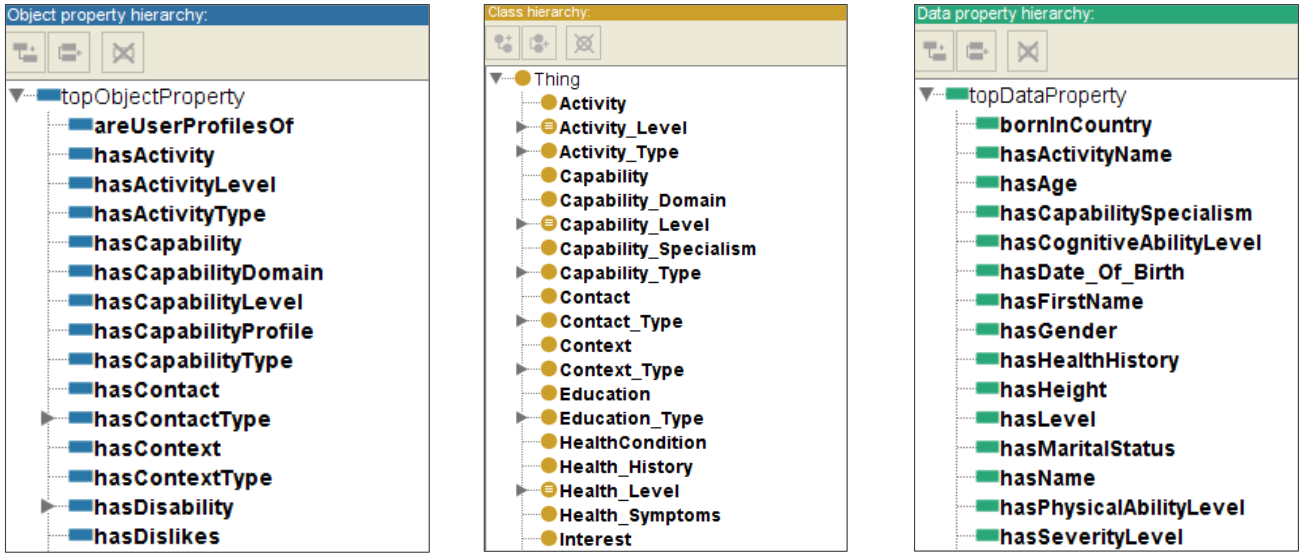
\includegraphics[width=0.70\textwidth]{skillen_ontology.png}
\caption{An overview of the User Profile Ontology classes, object properties and 
data properties~\citep{skillen2012ontological}.}
\label{fig:skillen_ontology}
\end{figure}

\subsubsection{Generic User Modelling Systems}
\label{sec:generic_users}

Apart from the analysed models there is another generic approach for modelling 
users known as Shell Systems. More focused in the field of \ac{ai}, these 
solutions consider the user model as a source of information which are built on 
assumptions about relevant user aspects or 
behaviour~\citep{pohl_logic_based_1999}.

\citet{heckmann_ubiquitous_2005} differentiates between the model, which is where 
the user data is collected, and the modelling system, which is the module that
manages the model. Besides, he remarks the following two definitions
from~\citet{wahlster_user_1989} previous work:

\begin{description}
  \item[\Defi{User Model (I), by~\citet{heckmann_ubiquitous_2005}}] \hfill \\
  \begin{mdframed}[hidealllines=true,backgroundcolor=gray!20]
  \textit{``A user model is a knowledge source in a system which contains explicit
  assumptions on all aspects of the user that may be relevant to the behaviour
  of the system. These assumptions must be separable by the system from the
  rest of the system's knowledge''}~\citep{wahlster_user_1989}.
  \end{mdframed}

  \item[\Defi{User Model (II), by~\citet{heckmann_ubiquitous_2005}}] \hfill \\
  \begin{mdframed}[hidealllines=true,backgroundcolor=gray!20]
  \textit{``A user modelling component is that part of a system whose function is to
  incrementally construct a user model; to store, update and delete entries;
  to maintain the consistency of the model; and to supply other components of
  the system with assumptions about the user''}~\citep{wahlster_user_1989}.
  \end{mdframed}
  
\end{description}


% % \begin{framed}
%   \begin{mydef}
%     {A user model is a knowledge source in a system which contains explicit
%     assumptions on all aspects of the user that may be relevant to the behaviour
%     of the system. These assumptions must be separable by the system from the
%     rest of the system's knowledge.~\citep{wahlster_user_1989}}
%   \end{mydef} 
% % \end{framed}
% 
% % \begin{framed}
%   \begin{mydef}
%     {A user modelling component is that part of a system whose function is to
%     incrementally construct a user model; to store, update and delete entries;
%     to maintain the consistency of the model; and to supply other components of
%     the system with assumptions about the user.~\citep{wahlster_user_1989}}
%   \end{mydef} 
% % \end{framed}

Assumptions are deeply studied and depicted in~\citep{pohl_logic_based_1999}. 
In this section, a quick overview of how these systems behave is performed to 
just take into account the difference between generic user modelling approach 
(user modelling shells) and the approach followed in this dissertation, which 
is related to Human-Computer Interaction.

In 1986 \ac{gums} is presented. This software allowed developers to make 
user-adaptive applications by defining several stereotypes, facts and rules to 
reason with~\citep{finin_gums_1986}. \acs{gums} supports the addition of new 
facts in runtime, manages facts inconsistencies and answers the application 
about assumptions about the user~\citep{kobsa_generic_2001}. The following 
systems are several examples of generic user systems developed in the following 
years (chronological ordered):

\begin{itemize}
  \item DOPPELGÄNGER, which uses several learning techniques for generalizing
  and extrapolating sensor data for the development of the user model
  \citep{orwant_doppelgangeruser_1991}.
  \item \ac{umt}, which supports the definition of hierarchically ordered 
  stereotypes about the user, rules for user model inferences and contradiction 
  detection~\citep{brajnik1994shell}.
  \item TAGUS, which uses first-order formulas to represent assumptions about
  the user~\citep{paiva1994tagus}.
  \item The um toolkit, which models not only assumptions but beliefs, preferences and other
  user characteristics in attribute-value pairs~\citep{kay1994toolkit}.
  \item BGP-MS, which permits user and groups of users assumptions~\citep{kobsa1994user}.
\end{itemize}

% MÁS SISTEMAS? SOLO LLEGAMOS A 1995\dots ESTOS SISTEMAS SON MUY ANTIGUOS, SI NO PONEMOS A
% PARTIR DEL 2000 MEJOR NI PONERLOS IGUAL\dots


% A significant aspect of these systems is that they are required to be usable in
% as many applications as possible. This is, domain independent. Therefore, they
% are expected to provide as many services as possible. On the contrary, in Human-Interaction
% user modelling approaches this is, in fact, an issue \citep{cita_falta_modelos_usuarios_comparar}.
% This problem is addressed in Chapter~\ref{cha:el_que_sea}.

% Domain independence
% 
% Known systems: 
% 
% GroupLens
% LikeMinds
% Personalization Server
% Frontmind
% Learn Sesame

% \InsertFig{heckmann_model}{fig:heckmann_model}{Several user model property dimensions \citep{heckmann_user_2007}}{}{0.70}{}

% ----------------------------------------------------------------------



\subsection{Users Models Comparison}
\label{sec:user_model_comparison}

In this section we describe our user modelling requirements nurtured by the 
earlier works described. As mentioned before, there are several perspectives 
regarding the user modelling requirements. In this dissertation the \ac{hci} 
perspective is taken. This means, as~\citet{pohl_logic_based_1999} states, 
that the user model refers to user characteristics using a certain system (see 
Section~\ref{sec:chronological_review}). In Chapter~\ref{cha:ontology_model}
the AdaptUI models for user, context and device are described. These models
have been designed considering each of these entities as a set of characteristics
that define them. Hence, the adaptation platform is able to evaluate the
combination of these characteristics and perform the corresponding adaptation.
Thus, the \ac{hci} interpretation of user modelling suits the goal pursued
by AdaptUI.

% Now that the \ac{hci} viewpoint has been remarked, we emphasize the amount of 
% different domains that are addressed in the literature considering user 
% modelling. 

In the following lines the amount of different domains addressing user modelling 
are highlighted. From product design to multimedia and user interfaces adaptation, 
every approach follows the same purpose: to consider several user characteristics 
to improve the system and user's satisfaction and product or service usability. 
However, although these solutions share the same objectives, the considered 
characteristics differ a lot. For ubiquitous and more context-aware domains, 
activities are taken into account. For example,
~\citet{razmerita_ontology_based_2003} discuss an ontology based architecture, 
which aims to be generic by collecting user data through two different ways 
(explicitly and implicitly).~\citet{golemati_creating_2007} also take an 
ontological point of view to avoid the problem of domain dependency (among 
others) by designing a more general, comprehensive and extensible ontology. 

\citet{gauch_ontology_based_2003} remark in the presented ontology the 
importance of time. Regarding the studied domain (web browsing) time is 
significant because it might help characterizing the user considering the spent 
time reading an article or visiting a website. Well known and popular 
recommendation systems, as YouTube, utilise this information combined with 
different explicit and implicit sources from the user interaction to make proper
recommendations~\citep{davidson_youtube_2010}.

User activities have also been considered as relevant for many authors in the 
literature. The first example is the Doppelgänger 
system~\citep{orwant_doppelgangeruser_1991} (1991), which uses activities for 
sharing relevant user information to different applications. In the same 
way,~\citet{persad_characterising_2007},~\citet{heckmann_gumogeneral_2005}
and~\citet{skillen2012ontological} modelled activities to take user's behaviour
and interaction into account for the proposed classifications and systems. For
~\citet{hatala_ontology_based_2005} activities are also vital within 
context-aware environments.

As occurs with context modelling (see Section~\ref{sec:context_model_comparison})
many different techniques are available for the model representation. This usually
depends either on the developer, because of his/her experience, or in the system's
technical characteristics. For example, if the system is able to performs inference
with the user data an ontology based representation could be more helpful than
an object based one.~\citet{strang_context_2004} demonstrated that ontological
modelling is more appropriate for ubiquitous computing environments.

It is also common to model physiological related characteristics of the user.
For example, the works by~\citet{gregor_designing_2002} 
and~\citet{persad_characterising_2007} consider physical, cognitive an sensory 
capabilities.~\citet{skillen2012ontological} also model several user abilities 
for performing different tasks and activities. The problem is that being aware 
of these capabilities is difficult and, in some cases, poorly practical. For 
example, measuring the sight capability of one individual requires physiological 
experience or advice. Besides, people with the same affection do not respond in 
the same way. A person who was born blind would interact differently with the 
environment than another who has been losing sight during his/her life. The 
precise same disability (e.g., tunnel vision) might affect different people 
in many different ways depending on their personal skills (e.g., adaptability,
orientation, and so forth). This might lead to an idea. What if, instead of 
modelling physiological skills (disabilities), we were able to model user's 
capabilities? The first approximation for this is found 
in~\citet{casas_user_2008} work. \citeauthor{casas_user_2008} present a user 
profile which abstracts from physiological aspects and lets users manage and 
configure their own profile. On the contrary, \citet{skillen2012ontological} 
model user capabilities as a set of abilities which allow users to perform some 
task or activities. Although this perspective covers many user capabilities, it
still needs a deeper understanding of physiological user capabilities.

On the other hand,~\citet{fischer_user_2001} comments that it not only is 
difficult to model users because of the wide range of different types of people 
that exist. He also considers that each individual changes with experience and 
through time. For example, old people's capabilities decrease with ageing. This
idea is shared with~\citet{gregor_designing_2002}, whose work is centred around
the elderly. \citet{heckmann_ubiquitous_2005} not only considers that users 
might evolve (from an \ac{ai} perspective), but he also takes new context 
information from the inference process. This also opens a new point of view 
that we address in Section~\ref{sec:context_disabilities} and it is about taking 
context as a significant user's environment entity that might directly influence 
the user's capabilities. In other words, users change through experience, time 
and, in concrete situations, due to the current context characteristics. For 
example, an individual might not suffer from any mobility disability, but in a 
crowded street would be difficult to perform several daily activities (just 
walking could be difficult).~\citet{razmerita_ontology_based_2003} also address 
this issue when they talk about the implicit user information collecting 
process. This, of course, deals with the concept of dynamism.

\citet{evers_achieving_2012} consider that respecting user's interactive 
behaviour with applications needs to be taken into account. On the other hand,
~\citet{pereira_triple_2005} analyses the differences between emotional and
perceptional user characteristics. 

% Several authors have also noticed the importance of tolerating the management of
% non-trustworthy data. Ambiguity and uncertainty mean working with data which might
% not reflect the current situation. Beynon et al. considered uncertainty as an actual
% problem to deal with \citep{beynon2000dempster}.

Table~\ref{tbl:user_comparison} summarizes the analysed approaches for user
modelling, emphasizing the modelled user characteristics and domains. 


% Besides, 
% although in a first version every used technique was remarked, in this 
% dissertation we focus on remarking just those which follow an ontology-based 
% approach. This is because many of the cited works are more theoretical or 
% surveys, or they just give some advices about important context data when 
% facing a context modelling task. Besides, \citet{strang_context_2004} 
% demonstrate that using ontologies is more appropriate for modelling 
% context-aware systems.

\begin{table}
  \caption{Related work for the user modelling approaches. Under the user
 characteristics heading \underline{A}ctivities or behaviour, \underline{C}apabilities,
 \underline{Ex}perience,  \underline{I}nterests, \underline{E}motions,
 \underline{P}ersonal, \underline{S}tress and \underline{L}ocation information
 are presented.}
 \label{tbl:user_comparison}
\footnotesize
\centering
 \begin{tabular}{l c c c c c c c c c}
  \hline 
  \textbf{Solution} & \textbf{Ontologies} & \multicolumn{8}{c}{\textbf{User characteristics}}\\
  \textbf{(Domain)} & & \textbf{A} & \textbf{C} & \textbf{Ex} & \textbf{I} & \textbf{E} & \textbf{P} & \textbf{S} & \textbf{L} \\
  \hline
  
  2002,~\citet{gregor_designing_2002}		&  		& & $\checkmark$ & $\checkmark$ & & & & & \\
  (Inclusive design)\\
  2003,~\citet{gauch_ontology_based_2003}	& $\checkmark$	& & & & $\checkmark$ & & & &\\
  (Automatic profiling)\\ 
  2003,~\citet{razmerita_ontology_based_2003}	& $\checkmark$	& $\checkmark$ & & & $\checkmark$ & & $\checkmark$ & & \\
  (\ac{kms})\\				
  2005,~\citet{hatala_ontology_based_2005} 	& $\checkmark$ 	& & & & $\checkmark$ & & $\checkmark$ & & $\checkmark$ \\
  (Tangible interfaces)\\		
  2005,~\citet{pereira_triple_2005} 		& 		& & & & & $\checkmark$ & & &  \\
  (Multimedia adaptation)\\
  2007,~\citet{persad_characterising_2007} 	&   		& $\checkmark$ & $\checkmark$ & & & & & & \\
  (Product design demands)\\
  2007,~\citet{golemati_creating_2007} 		&  $\checkmark$   	& $\checkmark$ & & $\checkmark$ & $\checkmark$ & & $\checkmark$ & & \\
  (User profiling)\\
  2007,~\citet{heckmann_gumogeneral_2005} 	& $\checkmark$   	& $\checkmark$ & & & & $\checkmark$ & $\checkmark$ & $\checkmark$ & \\
  (Ubiquitous applications)\\
  2008,~\citet{casas_user_2008} 		&  		& & $\checkmark$ & $\checkmark$ & & & & & \\
  (\ac{aui}\\
  2012,~\citet{evers_achieving_2012} 		&  		& & & & & & & $\checkmark$ & \\
  (Adaptive applications)\\
  2012,~\citet{skillen2012ontological} 		&  $\checkmark$	& $\checkmark$ & $\checkmark$ & & $\checkmark$ & & & & $\checkmark$ \\
  (Mobile environments)\\
  \hline

\end{tabular}
\end{table}



\section{Context Modelling}
\label{sec:context}
%------------------------------------------------------------------------- 
\subsection{What is context?}
\label{sec:context_definition}

% Context is mostly defined by the definition by Dey as follows:
Context is often defined according to \citeauthor{dey_understanding_2001}
issued definition:

\begin{description}
  \item[\Defi{Context (I), by~\citet{dey_understanding_2001}}] \hfill \\
  \begin{mdframed}[hidealllines=true,backgroundcolor=gray!20]
  \textit{`Context is any information that can be used to characterize the situation
  of an entity. An entity is a person, place, or object that is considered 
  relevant to the interaction between a user and an application, including the 
  user and applications themselves``}~\citep{dey_understanding_2001}.
  \end{mdframed}
\end{description}

In the past decades there were many definitions of context~\citep{adomavicius_context_aware_2011}.
Nevertheless, the one stated by~\citet{dey_understanding_2001} is one of the most
popular and extended definitions. \citeauthor{dey_understanding_2001}'s 
definition enables developers to easily enumerate those elements which take part 
in the context for a certain application domain. \citeauthor{dey_understanding_2001} stated that:

\begin{description}
  \item[\Defi{Context (II), by~\citet{dey_understanding_2001}}] \hfill \\
  \begin{mdframed}[hidealllines=true,backgroundcolor=gray!20]
  \textit{``If a piece of information can be used to characterize the situation 
  of a participant in an interaction, then that information is context''~\citep{dey_understanding_2001}}.
  \end{mdframed}
\end{description}

A proposed example explains this definition: \textit{``Take the canonical 
context-aware application, an indoor mobile tour guide. The obvious entities in 
this example are the user, the application and the tour sites. We will look at 
two pieces of information – weather and the presence of other people – and use 
the definition to determine whether either one is context. The weather does not 
affect the application because it is being used indoors. Therefore, it is not 
context. The presence of other people, however, can be used to characterize the 
user's situation. If a user is travelling with other people, then the sites they 
visit may be of particular interest to her. Hence the presence of other people 
is context because it can be used to characterize the user's situation.''~\citep{dey_understanding_2001}}

By this example, it is seen how different pieces of information are analysed to
determine if they belong to what \citeauthor{dey_understanding_2001} states 
context is. These definitions are based on research experience. 
Section~\ref{sec:context_models} shows how modelling and defining context has 
evolved in the past 20 years. 

% Context management allows us to identify the conditions of the environment. This
% way, developers are able to adapt services or applications for the user taking
% into account these conditions. To do this first there is the need of gathering
% context information. Next this information has to be somehow processed and,
% finally, it will be used to personalize and contextualize the current situation.

% ----------------------------------------------------------------------

\subsection{A Chronological Review of the Evolution of Context Management}
\label{sec:chronological_review}
% \dots
The following figure shows the evolution for context modelling by chronological
order for the last 15 years. 

\vspace{1cm}
\setlength\taskwidth{1.7cm}

\begin{timeline}
  \label{chr:context}
    \Task[2000]{\citet{chen_survey_2000}}
    \Task[2001]{\citet{jameson_modelling_2001}}
    \Task[2002]{\citet{henricksen_modeling_2002}, \citet{held_modeling_2002}}
    \Task[2004]{\citet{gu_toward_2004}}
    \Task[2005]{\citet{chen_using_2005}, \citet{yamabe_citron_2005}}
    \Task[2008]{\citet{wood_context_aware_2008}}
    \Task[2011]{\citet{baltrunas_incarmusic_2011}}
    \Task[2012]{\citet{mcavoy_ontology_based_2012}}
    \Task[2013]{\citet{almeida_assessing_2012}}
\end{timeline}


\subsection{Context models}
\label{sec:context_models}

The first definition of \textit{context-aware systems} is given by~\citet{schilit_disseminating_1994}.
\citet{dey_understanding_2001} also defines \textit{context-aware systems} as
those systems which, using context data, provide significant information and/or
services to the user where the relevancy of the given information depends on the
user task.~\citet{schmidt_there_1999} consider several issues about context
modelling. Authors emphasize the excess of abstraction about context-aware systems
and environments which causes a lack of models to be compared . Therefore they
present a working model for context-aware systems categorized into human and
physical environment factors. In 2001~\citet{jameson_modelling_2001} studies how
context-aware computing represents a challenging frontier for researchers. In
this work, information about the environment, the user current state, longer
term user properties and the user behaviour are compared in order to take the
correct adaptation decision. Several works focused on user interface adaptation
area base their processes on context changes as triggers. However, they lack of
a common model of context in their platforms~\citep{calvary_plasticity_2002}
~\citep{nilsson_model_based_2006}.
% This fact emphasizes the argument established by Schmidt et al. \cite{schmidt_there_1999}.

In the following subsections a review of the most popular context-aware systems
is presented, mainly focusing on the modelled context parameters, techniques, 
domains and dependencies. Besides, several authors define context and 
context-awareness through their own experience. All these models and definitions 
have been considered for the context model proposed in 
Chapter~\ref{cha:ontology_model}. In Section~\ref{sec:context_model_comparison} 
Table~\ref{tbl:context_comparison} shows several significant features of each 
approach, and a comparing analysis is performed.


\subsubsection{2000: Chen and Kotz}
%\cite{chen_survey_2000}
\label{sec:chen}

\citet{chen_survey_2000} define context as follows: 

\begin{description}
  \item[\Defi{Context, by~\citet{chen_survey_2000}}] \hfill \\
  \begin{mdframed}[hidealllines=true,backgroundcolor=gray!20]
  \textit{``Context is the set of environmental states and settings that either 
  determines an application’s behaviour or in which an application event occurs 
  and is interesting to the user''}~\citep{chen_survey_2000}.
  \end{mdframed}
\end{description}

Besides, the definition of active and passive context-aware computing is also 
given. To \citeauthor{chen_survey_2000}, active context awareness is:

\begin{description}
  \item[\Defi{Active Context Awareness}] \hfill \\
  \begin{mdframed}[hidealllines=true,backgroundcolor=gray!20]
  \textit{``(\dots) an application automatically adapts to discovered context, by the 
  changing in the application's behaviour''}~\citep{chen_survey_2000}.
  \end{mdframed}
\end{description}

On the contrary, they define passive context awareness as:

\begin{description}
  \item[\Defi{Passive Context Awareness}] \hfill \\
  \begin{mdframed}[hidealllines=true,backgroundcolor=gray!20]
  \textit{``(\dots) an application presents the new or updated context to an interested
  user or makes the context persistent for the user to retrieve later''}~\citep{chen_survey_2000}.
  \end{mdframed}
\end{description}

Based on the work by~\citet{schilit_context_aware_1994},~\citet{chen_survey_2000}
consider time as an important and natural context feature for many 
applications. Besides, they introduce the term \textit{context history}, which 
is an extension of the time feature recorded across a time span.

A significant problem remarked in this work is the impossibility to exchange
context information between the studied context-aware systems due to the way
they model the environment. Furthermore, as location is one of the most 
modelled context features, \citeauthor{chen_survey_2000} provide a study of 
several aspects that should be taken into account when researchers face the 
problem of modelling it. 

% \begin{table}[htbp]
% \caption{Data structures \cite{chen_survey_2000}}
% \label{tbl:chen}
% \begin{tabular}{ll}
% Technique & Description  \\
% \hline
% Key-value pairs & Used by Schilit et al. \cite{schilit_context_aware_1994}, \\
%  & an environmental variable acts as the key while the \\
%  & actual context data is the value. \\
% Tagged encoding & Used by P.J. Brown \cite{brown_stick-e_1995}, the \\
%  & contexts are modeled as tags and corresponding \\ 
%  & fields. \\
% Object-oriented model & The systems that use this technique usually \\
%  & consider the contextual information as the states \\ 
%  & of the object and the object provides methods to \\ 
%  & access and modify these states \\
% Logic-based model & Context data can be expressed as facts in a \\
%  & rule-based system. \\
% % Others & Lightning \\
% \end{tabular} 
% \end{table}


% ----------------------------------------------------------------------


\subsubsection{2001: Anthony Jameson}
%\cite{jameson_modelling_2001}
\label{sec:jameson}

\citet{jameson_modelling_2001} analyses in 2001 how context-aware computing 
represents a challenging frontier for researchers in the field of \acp{aui}. 
In this work information about the environment, the user's current 
state, longer term user properties and the user behaviour are compared in order 
to take the correct adaptation decision. The idea is to compare several 
scenarios. In the first one, only information about the environment is 
considered. In the following scenarios the user's current state, behaviour and 
long-term properties are taken into account. Thus, the results conclude 
that considering a wider range of user information can help context-aware 
systems designers.

% Table~\ref{tbl:jameson} shows the context parameters modeled by Jameson:
% 
% \begin{table}[htbp]
% \caption{Modeled context parameters \cite{jameson_modelling_2001}}
% \label{tbl:jameson}
% \begin{tabular}{ll}
% Scenario & Modeled parameters  \\
% \hline
% Using only information about & Location (GPS or similar readings) \\
% the environment & \\
% 
% Adding the user's current state & Emotional arousal \\
% Adding the user's behavior & Cognitive load, \\
%  & Current Goal \\
% Adding long-term user properties & Personal characteristics, \\
%  & Knowledge, Interests, Noncognitive Abilities \\
% 
% \end{tabular} 
% \end{table}

% ----------------------------------------------------------------------


\subsubsection{2002: Henricksen et al.}
\label{sec:henricksen}
% MENCIONAR TAMBIÉN SU TRABAJO EN 2003.

The approach followed by~\citet{henricksen_modeling_2002} makes the following
notes about context in pervasive environments:

\begin{itemize}
  \item Context information exhibits \textit{temporal characteristics}. Context 
  can be  static (e.g., birthday) or dynamic (e.g., user location). Besides, the 
  persistence of the dynamic information can easily change. Thus, it is justified 
  that the static context should be provided by the user, while the dynamic 
  one should be gathered by sensors. Past historic and a possible forecasting 
  of future context are also taken into account as part of the description of 
  the whole context description.
  
  \item A second property of the context information is its \textit{imperfection}. 
  Information can be useless if it cannot reflect a real world state. It also 
  can be inconsistent if it contains contradictions, or incomplete if some 
  context aspect are unknown. There are many causes to these situations. For 
  example, information can change so fast that it may be invalid once it is 
  collected. This is obviously because the dynamic nature of the environment. 
  Besides, there is a strong dependency on software and hardware infrastructures, 
  which can fail any time.
  
  \item Context has \textit{multiple alternative representations}. Context 
  information usually comes from sensors which speak different languages. For 
  example, a location sensor can use latitude and longitude physical magnitudes 
  while the involved application works with a logical representation of location. 
  
  \item \textit{Context information} is highly \textit{disassociated}. There are 
  obvious connections between some context aspects (e.g., users and devices). 
  However, other connections need to be computed with the available information.
\end{itemize}

% \The Figure~\ref{fig:henricksen} shows the annotated context model designed by Henricksen et al.
This work also indicates the dependency between context models, the scenarios 
and use cases of the application domains. Authors extract several context 
parameters to consider:

\begin{itemize}
  \item User activity, distinguishing between the current one and the planned one.
  \item Device that is being used by the user.
  \item Available devices and resources.
  \item Current relationships between people.
  \item Available communication channels.
\end{itemize}

% \InsertFig{henricksen}{fig:henricksen}{Context model annotated with quality parameters and metrics \cite{henricksen_modeling_2002}}{}{0.70}{}

% 
% \subsubsection{2003, Henricksen et al.}
% %\citep{henricksen_generating_2003}
% \label{sec:henricksen}
% 
% Henricksen et al. discuss about the difficulties of constructing context-aware
% applications. Besides, they remark the lack of formality and expressiveness of
% previous context-aware solutions and models. For example, several specific context
% information, as histories, uncertainty, incompleteness, sensor-derived information
% and different kind of dependencies between the information are barely conceptually 
% modeled with ER or UML approaches, which are not well suited for this task \citep{henricksen_generating_2003}.
% Therefore, they present a context modeling approach which allows developers to describe high level context
% information. In addition, a mapping process for transforming high-level context
% models to management systems is also described. This way, they characterize the
% Object-Role Modeling approach to support specific context information based
% on abstraction concepts and quality annotations. 
% 
% Authors classify context into static or dynamic facts\dots
\subsubsection{2002: Held et al.}
% \citep{held_modeling_2002}
\label{sec:held}

In 2002~\citet{held_modeling_2002} discussed about the necessity of content 
adaptation and representation formats for context information in dynamic 
environments. A significant perspective is the justification of modelling not 
only the user but the network status and device context information as well.
The following parameters are considered as relevant context information:

\begin{itemize}
  \item \textit{Device}: basic hardware features (e.g., \acs{cpu} power, memory 
  and so forth), user interface input (e.g., keyboard and voice recognition), 
  output (e.g., display and audio), and other particular specifications of the 
  device (e.g., display resolution or colour capability).
  \item \textit{User}: service selection preferences, content preferences and 
  specific information about the user.
  \item \textit{Network connection}: bandwidth, delay, and bit error rate. 
\end{itemize}

Authors also present several requirements concerning the representation of
context information. Accordingly, they defend that a context profile should be:

\begin{itemize}
  \item Structured, to ease the management of the amount of gathered information
  and remark relevant data about the context.
  \item Interchangeable, for components to interchange context profiles.
  \item Composable/decomposable, to maintain context profiles in a distributed way.
  \item Uniform, to ease the interpretation of the information.
  \item Extensible, for supporting future new attributes.
  \item Standardized, for context profile exchanges between different entities
  in the system.
\end{itemize}
\subsubsection{2004: Gu et al.: The \ac{socam} Ontology}
\label{sec:gu}

In 2004~\citet{gu_toward_2004} design \ac{socam} architecture for designing and 
prototyping applications in an \ac{ie}. Built on top of the 
\ac{osgi}\footnote{www.osgi.org} architecture, such middleware consisted of the 
following components:

\begin{itemize}
  \item Context providers, which abstract context information from heterogeneous
  sources and semantically annotate it according to the defined ontology.
  \item The context interpreter, which provides logic reasoning to process
  information about the context.
  \item The context database, which stores current and past context instance data.
  \item Context-aware applications, which adapt their behaviour according to the
  current context situation.
  \item The service-locating service, which allows context providers and 
  interpreters to advertise their presence for users and applications to locate 
  them.
\end{itemize}

\citeauthor{gu_toward_2004} use \ac{owl} to describe their context ontologies 
in order to support several tasks in \ac{socam}. As the pervasive computing 
domain can be divided into smaller sub-domains, the authors also divided the 
designed ontology into two categories: 

\begin{itemize}
  \item An \textit{upper ontology}, which captures high-level and general 
  context knowledge about the physical environment.
  \item A \textit{low-level} ontology, which is related to each sub-domain and 
  can be plugged and unplugged from the upper ontology when the context changes.
\end{itemize}

As a result, the upper ontology considers person, location, computational entity
and activity as context concepts.

\citet{gu_ontology_based_2004} also present an \ac{owl} based model to represent, 
manipulate and access context information in smart environments. The model 
represents contexts and their classification, dependency and quality of
information using \ac{owl} to support semantic interoperability, contextual 
information sharing, and context reasoning. The ontology allows to associate 
entities' properties with quality restrictions that indicate the contextual 
information quality. 
\subsubsection{2005: Chen et al.: The \ac{cobra} Ontology}
\label{sec:gu}

Another work under a similar approach is the one performed by~\citet{chen_using_2005}.
Authors introduce the \ac{cobra} ontology based system, which provides a set of 
semantic concepts for characterizing entities such as people, places or other 
objects within any context. The system provides support for context-aware 
platforms in runtime, specifically for Intelligent Meeting Rooms. The context 
broker is the central element of the architecture. This broker maintains and 
manages a shared context model between agents (applications, services, web 
services, and so forth) within the community. In intelligent environments participating
agents often have limited resources and capabilities for managing, reasoning and
sharing context. The broker's role is to help these agents to reason about the
context and share its knowledge. The presented ontology relies on:

\begin{itemize}
  \item Concepts that define physical places and their spatial connections.
  \item Concepts that define agents (humans and not humans).
  \item Concepts that define the location of an agent.
  \item Concepts that describe an agent activity.
\end{itemize}
\subsubsection{2005: Yamabe et al.: The Citron Framework}
%\cite{yamabe_citron:_2005}
\label{sec:yamabe}

In 2005~\citet{yamabe_citron_2005} present a framework for personal devices 
which gathers context information about the user and his/her surrounding 
environment. Muffin, a personal sensor-equipped device is designed. Using it, 
several context parameters are gathered.

Sensor information is also considered for evaluating several user high-level 
context information. For example, accelerometer readings might recognize a 
walking or running activity, shaking and rotating, an so forth. The microphone 
is not only used to measure the ambient noise. It is also useful for detecting 
the place where the user is (e.g., meeting room, restaurant, street and so on).

The context acquisition is categorized in two different groups: the user and 
the environment. For the user several issues are analysed. For example, 
activity recognition requires the user to use the device in specific ways (it 
is not the same to use it with hands or waist-mounted). Another problem they 
encounter is about the time consuming process since an event is captured, then 
processed and finally validated. The last contextual issue deals with the 
intrinsic complexity and ambiguity of context information. For example, the 
meaning of what is loud might depend on the current situation (e.g., if the 
user is in a meeting room, if the user is in the street, and so on). For the 
environment, Muffin suffer several heat problems due to the sensors sensitivity
to environment temperature. This way, sometimes the gathered measures are invalid.

% \begin{table}
% \caption{Modeled context parameters \cite{yamabe_citron:_2005}}
% \label{tbl:yamabe}
% \begin{tabular}{ll}
% Sensor category & Modeled parameters  \\
% \hline
% Environmental sensors & Air temperature \\
%  & Relative humidity \\ 
%  & Barometer \\
%  
% Physiological sensors & Alcohol gas \\
%  & Pulse \\
%  & Skin temperature \\
%  & Skin resistance \\
% 
% Motion/location sensors & Compass/tilt \\
%  & 3D accelerometer \\
%  & Grip \\
%  & Ultrasonic range finder \\
%  & GPS \\
% 
% Other sensors & RFID tags \\
%  & Front rear images \\
%  & Sound \\
% \end{tabular} 
% \end{table}
\subsubsection{2008: Wood et al. and the AlarmNet system}
% \cite{wood_context-aware_2008}
\label{sec:wood}

AlarmNet is an \ac{aal} \ac{wsn} for pervasive adaptive healthcare in assisted 
living residences for patients with special needs. In this 
work,~\citet{wood_context_aware_2008} contribute with several novelties:

\begin{itemize}
  \item An extensible heterogeneous network middleware.
  \item Novel context-aware protocols.
  \item SenQ, a query protocol for efficiently streaming sensor data.
\end{itemize}

The context-aware protocol uses a two-way network information flow. On the one 
hand, environmental, system and residents data flow. On the other hand, \ac{car} 
analysis goes back into the system to enable smart power management and dynamic 
alerts.

Several sensors are used for sensing environmental quality: light, temperature,
dust, resident activities (motion sensors) and so on. The devices' queries to the 
system are negotiated by the Query Manager.
\subsubsection{2011: Baltrunas et al.: InCarMusic}
%\cite{baltrunas_incarmusic_2011}
\label{sec:baltrunas}

Assuming that context-aware systems adapt to the specific user situation,
\citet{baltrunas_incarmusic_2011} present a music recommendation system which
takes into account the user's mood and the traffic conditions. To this
end, the authors design a methodology where users can be requested to judge several
contextual factors (e.g., if current traffic conditions are relevant for a decision
making task) and to rate an item when a certain contextual condition is met. 

In order to take into account the user's music preference and the influence that
context might have into them, context is modelled as several independent factors.
% (see Table~\ref{tbl:baltrunas}).
% 
% \begin{table}
% \caption{Modeled context parameters \cite{baltrunas_incarmusic_2011}}
% \label{tbl:baltrunas}
% \begin{tabular}{ll}
% Contextual factor & Contextual conditions  \\
% \hline
% Driving style & Relaxed driving \\
%  & Sport driving \\
% Road type & City \\
%  & Highway \\
%  & Serpentine \\
% Landscape & Coast line \\
%  & Country side \\
%  & Mountains/hills \\
%  & Urban \\
% Sleepiness & Awake \\
%  & Sleepy \\
% Traffic conditions & Free road \\
%  & Many cars \\
%  & Traffic jam \\
% Mood & Active \\
%  & Happy \\
%  & Lazy \\
%  & Sad \\
% Weather & Cloudy \\
%  & Snowing \\
%  & Sunny \\
%  & Rainy \\
% Natural phenomena & Day time \\
%  & Morning \\
%  & Night \\
%  & Afternoon \\
%   
% \end{tabular} 
% \end{table}
\subsubsection{2012: McAvoy et al.}
\label{sec:mcavoy}

\citeauthor{mcavoy_ontology_based_2012} propose an ontology-based system for the 
managing of context within smart environments. One of the most significant 
contributions deals with the high-level information managed through the metadata 
and meaning which are collected by the sensor network~\citep{mcavoy_ontology_based_2012}. 
The sensing devices within the smart environment have to be modelled in order 
to be semantically enriched. Data is formally represented as an ontology by 
using entities and the relationships which link them together. After the data 
is collected from the sensors it is passed to an enrichment module where it is 
made semantically rich. This new enriched data is stored in a semantic 
repository in the form of triples. The meaning of this information and the 
metadata are added to the data within this enrichment component. 

\subsubsection{2013: Almeida and López-de-Ipiña: The AMBI2ONT Ontology}
\label{sec:almeida}

\citet{almeida_assessing_2012} consider two common problems dealing with 
ambiguity in the area of context modelling: the uncertainty and the vagueness. 
Uncertainty models the likeness of a certain fact, while the vagueness 
represents the degree of membership to a fuzzy set. The uncertainty is 
represented by a certainty factor.

Due to the nature of the process of collecting data from the environment, the
proposed ontology has been designed to support two types of uncertainty:

\begin{itemize}
  \item Uncertain data: This kind of uncertainty is generated from the capture
  of data from sensors due to the imperfect nature of the devices.
  \item Uncertain rules: It occurs in the execution of the rules. 
\end{itemize}

To reason over the ambiguous information the JFuzzy Logic Open Source fuzzy
reasoner has been adapted to support uncertainty information.



\subsubsection{Context Models Comparison}
\label{sec:context_model_comparison}

The previous section has reviewed several significant context-aware systems and 
the followed approaches for modelling relevant context parameters of the environment
depending on the application domain. In fact, this is one of the main problems in
context modelling: the lack of model independence from similar domains and, also,
the lack of models to be compared. Despite the fact that sometimes the primary
domains are similar (context-aware computing, pervasive environments and ubiquitous
computing) regarding the necessity of managing context knowledge, the concrete
applications and approaches' domains are different. 
Here,~\citet{henricksen_modeling_2002} realize about the lack of formality and 
expressiveness of previous context models.

However, to avoid this problem~\citet{gu_ontology_based_2004} present an
ontology-based solution in which context information is modelled in two separated
layers:

\begin{itemize}
  \item In the upper layer there is an ontology which describes high-level 
  knowledge about the current context and physical environment.
  \item Under it there is the possibility to add and remove ontologies which
  model low-level information of the current specific domain.
\end{itemize}

On the one hand, this approach allows developers to consider richer information,
as activities, and abstract knowledge about the current global context. On the
other hand, it makes possible to model specific knowledge of the current sub-domain.
Besides, the possibility to plug and unplug these low-level ontologies makes this
solution powerful. The solution provided by~\citet{gu_toward_2004} is significant
because of the following reasons:

\begin{itemize}
  \item It considers high-level information on top of a more specific and domain
  dependent sub-model. 
  \item Activities are modelled as a relevant concept for context in the upper
  ontology.
  \item The modelled entities are related. Persons are associated with locations
  and activities, each location is linked with indoor or outdoor entities, 
  activities can be categorized into scheduled or deduced ones, and so forth. 
\end{itemize}

\citet{chen_survey_2000} survey several context-aware computing solutions. The 
remarked context characteristics (\textit{location} and \textit{time}) are given 
more as an advice, since they do not provide a reference model. Nevertheless, 
they introduce several novelties like the term \textit{context history}, which 
might be useful for future predictions about user's behaviour and trends.

Modelling high-level information allows to perform deeper computations taking
into account behavioural characteristics, trends information, inferred knowledge
from small pieces of information combinations, and so on. As can be seen in
Table~\ref{tbl:context_comparison} many authors work with high-level data in 
their context-aware systems. 

On the other hand, physical context parameters are frequently modelled in the
analysed literature. \textit{Location}, \textit{time} and \textit{environment 
conditions} (e.g., temperature, pressure, light and noise) are usually modelled 
to achieve final system's goal (e.g., adapting the user interface or recommending 
items or services). Besides, several approaches take user related characteristics 
to fulfil their purposes. For example,~\citet{schmidt_there_1999} consider not 
only physical environment as context information but also several human factors 
categorized as follows:

\begin{itemize}
  \item User information, which gathers knowledge about user's habits, emotional
  stated and bio-physiological conditions.
  \item Social environment, made up by other user's locations, social interactions
  of the current user and knowledge about the behaviour of groups of people.
  \item Task, taking into account spontaneous activities, engaged tasks and 
  general goals.
\end{itemize}

A user modelling approach which considers emotional issues of the user is 
presented by~\citet{pereira_triple_2005}. The author distinguishes between 
emotions and perceptions to separate both concepts for modelling processes. 
These approaches are found useful for recommending systems in which user mood 
and psychological state are relevant to filter multimedia content 
\citep{baltrunas_incarmusic_2011}. Following a similar perspective~\citet{evers_achieving_2012}
analyse the user's participation in adaptive applications. Several concepts that
should be taken into account regarding the user behaviour and interaction with
the application are presented. Another similar approach regarding the user's more 
psychological aspects is presented by~\citet{liao_decision_2005}. Here the 
authors present a model for modelling user stress levels. This is related to the 
concept of Considerate Computing, term that it is explained in~\citep{gibbs_considerate_2005}.

\citet{schmidt_there_1999} also remark the social environment as relevant for 
context modelling. More related to recommending environments, non explicit 
information about user's likes need to be computed. Similar approaches in these 
environments tend to avoid recommending systems intrinsic problems, like the 
so-called \textit{cold start problem}~\citep{castillejo_alleviating_2012}\citep{castillejo_social_2012}.

Another relevant point remarked by~\citet{schmidt_there_1999} are the user's tasks.
Several authors consider activities relevant for modelling context 
\citep{henricksen_modeling_2002}\citep{gu_toward_2004}\citep{abowd_towards_1999}.
Activities enrich context information about the user~\citep{razmerita_ontology_based_2003}.
It is common to model user activities in the user model (see Table~\ref{tbl:user_comparison}). 
% However,
% taking into account that these activities are identified by sensors and with the
% interaction with the environment, the proposed model for context considers them
% as a context parameter. In addition, the followed perspective takes into account
% activities as an abstract term. The context model in this dissertation does not
% model individual activities but those situations in which the user can not achieve
% the final goal. This is explained with more detail in Section~\ref{sec:stressful_activities}.

Finally, sometimes the collected data might lead to misunderstandings or 
non-trustworthy data.~\citet{almeida_assessing_2012} consider \textit{ambiguity}
and \textit{uncertainty} in their work and present an ontology-based process 
which allows to model them within a smart environment.

\bigskip

Table~\ref{tbl:context_comparison} shows the differences between each reviewed
solution for modelling context. It is difficult to gather all the approaches in a
unique table. Therefore, Table~\ref{tbl:context_comparison} just emphasizes several
differences, although these solutions have more characteristics modelled. For example,
the work by~\citet{almeida_assessing_2012} is focused on modelling context uncertainty
and vagueness due to the nature of context data from sensors.

Besides and as it is deeply discussed by~\citet{strang_context_2004}, modelling 
the context with ontologies offers the following advantages:
\begin{itemize}
  \item Ontologies are the most expressive approach to model context.
  \item Composition and management of the model can be done in a distributed
  manner.
  \item It is possible to partially validate the contextual knowledge.
  \item One of the main strengths of ontologies is the simplicity to enact the
  normalization and formality of the model.
\end{itemize}

Regarding the context-aware systems, we cannot go further without remarking the 
issues of gathering information from different sources or sensors. This 
information might sometimes be unreliable. Sensors can fail in the collecting 
process, they also can stop working due to several reasons (e.g., power or 
malfunction). What is more, every sensor speaks its language (this issue is 
addressed applying different techniques, like data fusion). Therefore, a process 
to evaluate the quality and trustworthiness of the collected information should 
be included in every context-based system as a method to avoid undesired results.

\begin{table}
 \caption{Related work for context modelling approaches.}
 \label{tbl:context_comparison}
 \footnotesize
 \centering

\begin{tabular}{l c c c c c c c c c c c }
  \hline 
 \textbf{Solution} & \textbf{Ontologies} & \multicolumn{10}{c}{\textbf{Context parameters}} \\
 
 \textbf{(Domain)} & & \textbf{L} & \textbf{T} & \textbf{A} & \textbf{R} & \textbf{P} & \textbf{E} & \textbf{S} & \textbf{I} & \textbf{U} & \textbf{H}\\
    \hline 
        
    2000,~\citet{chen_survey_2000} 		&  & $\checkmark$ & $\checkmark$ &  &  &  &  &  &  &  &  \\
    (Context awareness)\\
    2001,~\citet{jameson_modelling_2001} 	&  & $\checkmark$ &  & $\checkmark$ &  &  &  &  &  & $\checkmark$ & $\checkmark$ \\
    (Context modelling)\\
    2002,~\citet{henricksen_modeling_2002} 	&   &  &  & $\checkmark$ & $\checkmark$ &  &  & $\checkmark$ & $\checkmark$ &  & $\checkmark$ \\
    (Pervasive computing)\\
    2002,~\citet{held_modeling_2002} 		&  &  &  &  &  &  &  &  & $\checkmark$ & $\checkmark$  &  \\
    (Context awareness)\\
    2004,~\citet{gu_toward_2004} 		& $\checkmark$ &  &  &  &  &  &  &  &  &  & $\checkmark$ \\
    (Smart environments)\\
    2005,~\citet{chen_using_2005} 		& $\checkmark$ & $\checkmark$ & $\checkmark$ & $\checkmark$ & $\checkmark$ & $\checkmark$ & $\checkmark$ &  & $\checkmark$ & $\checkmark$ & \\
    (Pervasive computing)\\
    2005,~\citet{yamabe_citron_2005} 		&  & $\checkmark$ &  & $\checkmark$ &  &  & $\checkmark$ &  &  & $\checkmark$ & $\checkmark$ \\
    (Mobile computing)\\
    2008,~\citet{wood_context_aware_2008} 	&  &  &  & $\checkmark$ &  &  & $\checkmark$ &  &  & $\checkmark$ &  \\
    (\ac{aal})\\
    2011,~\citet{baltrunas_incarmusic_2011} 	&  &  &  &  &  &  & $\checkmark$ &  &  & $\checkmark$ &  \\ 
    (Recommender systems)\\
    2012,~\citet{mcavoy_ontology_based_2012} 	& $\checkmark$ &  &  &  &  & $\checkmark$ &  &  &  &  & $\checkmark$  \\
    (Smart environments)\\
    2013,Almeida and	& $\checkmark$ & $\checkmark$ &  &  &  &  & $\checkmark$ &  &  &  &  \\
    López-de-Ipiña~\citep{almeida_assessing_2012}\\
    (Smart environments)\\
\hline

\end{tabular}
\end{table}

\subsubsection{Modelling Techniques}
\label{sec:modelling_techniques}

\citet{strang_context_2004} reviewed the context modelling literature in 2004.
They differentiate among several paradigms. Here we discuss several previously 
used context modelling techniques.


\myparagraph{Key-value}

\citet{maass_location_aware_1998} adopted a X.500 based solution to store location 
data. This approach is also used in distributed searching systems. Although it 
is very easy to maintain and handle its main problem is that it makes difficult 
to build complex structures~\citep{strang_context_2004}. Similar solutions follow 
this key-value approach to identify a context element (key), like location, with 
an environment variable (value)~\citep{schilit_customizing_1993}~\citep{voelker_mobisaic_1996}.

\myparagraph{Markup scheme}

Based on several derivative \ac{sgml}, for example \ac{xml}, marking schemes 
based models are widespread for modelling profiles. Some extensions are defined 
as \ac{ccpp} \footnote{http://www.w3.org/Mobile/CCPP/} standards and 
\ac{uaprof} \footnote{http://www.mobilemultimedia.be/en/uaprof/}. This kind of 
context modelling usually extends and completes the \ac{ccpp} and \ac{uaprof} 
basic vocabularies. In~\citep{held_modeling_2002} authors present an extension 
of this model, \ac{cscp}, which provides hierarchy to such schemes supporting 
the \ac{rdf} flexibility to express natural structures of profile information.

\myparagraph{Graphic models}

While~\citet{bauer_identification_2003} used a \ac{uml} tool to model the context in
a air traffic domain,~\citet{henricksen_generating_2003} presented a graphic model
(as an extension of Object-Role Modelling\footnote{http://www.orm.net/}). 
\ac{uml} is a widespread general purpose modelling tool with a very powerful 
graphic component (graphic models): the \ac{uml} diagram. 

\myparagraph{Object oriented models}

\citet{strang_context_2004} presented an object oriented model in which context
process details are embedded into object level. Data is hidden from other components.
Therefore, the access to this context data is just allowed through several interfaces.
This approach tries to use the object oriented programming benefits, as re-usability
and encapsulation, to cover ubiquitous environment's problems about context. Another
example of this approach is the one given by the GUIDE project by~\citet{cheverst_design_1999},
which is focused on location. In this case the context information is also in the
object as accessible states through those methods defined by the object itself
and by modifying these states.

% \paragraph{Logic models}

\myparagraph{Ontology based models}

As~\citet{strang_context_2004} discussed, modelling the context with
ontologies offers the following advantages:
\begin{itemize}
  \item Ontologies are the most expressive approach to model context.
  \item Composition and management of the model can be done in a distributed 
  manner.
  \item It is possible to partially validate the contextual knowledge.
  \item One of the main strengths of ontologies is the simplicity to enact 
  the normalization and formality of the model.
\end{itemize}

Multiple ontology based context models have been developed in the past. In the 
following section several ontology-based relevant models will be discussed.



% ----------------------------------------------------------------------



\section{Device Models}
\label{sec:devices}

There are many and different approaches in the literature for devices modelling.
Devices capabilities might determine the boundaries of an adaptation process or
the consumable resources.~\citet{lemlouma_context_aware_2004} considered that
an independent device model would probably reduce adaptation process efforts for
different context situations. In fact, \ac{w3c} reinforces this perspective
by warning about the wide range of device capabilities and 
sizes~\citep{device_independence} which define the boundaries of the content
that each device can handle. Several techniques, like Device Descriptors, content
transformation guides, devices \acp{api} and \ac{ccpp} systems help developers 
to optimize the user experience. These modelling techniques are analysed in the 
following section. 

\subsection{Composite Capabilities/Preference Profiles}
\label{sec:ccpp}
\ac{ccpp}~\citep{ccpp_status} is a \ac{w3c} standard system to express user and 
device capabilities. Using \ac{ccpp} a user will be able to show a specific 
preference or disability. For example, even though a user's device can display 
millions of colours, perhaps the user can just distinguish between a small set 
of colours. The necessity of this system stems from the wide range of web and 
ubiquitous devices available in the market. These devices have more and more 
multimedia and Web capabilities. This makes troublesome to Web content providers 
to service their content to these devices keeping usability and user 
satisfaction~\citep{lemlouma_context_aware_2004}. 

However, managing a large number of devices is not a new problem. Many approaches 
have been proposed in the literature to tackle this situation. Most of them are 
based on content management. This approach considers different presentation 
alternatives. Depending on the client device, a presentation configuration is 
served. Hence, in the content serving process there are two options: the 
server chooses which is the best configuration for the device, and the client 
decides what to do with the content. This approach is very easy to implement, 
since every device identifies itself against the server.

\ac{ccpp} is based on \textit{profiles}. A profile contains components and attributes.
Each component has, at least, one attribute, and each profile has at least one
component. The main components are: the hardware platform, the software platform
and single applications (e.g., a browser). Attributes can contain one or many 
values. For example, in case of the hardware platform component we can find the 
attributes \textit{displayWidth} and \textit{displayHeight}. These attributes 
have a single value. \ac{ccpp} uses \ac{rdf} as formal language to build these 
profiles. Table~\ref{tbl:ccpp} shows several advantages and drawbacks of this 
approach.



\begin{table}
\caption{\ac{ccpp}: several advantages and drawbacks}
\label{tbl:ccpp}
\footnotesize
\centering
\begin{tabular}{l l}
  \hline
  \textbf{Advantages}				& \textbf{Drawbacks}			\\
  \hline
  A good infrastructure for modelling devices 	& Device dependent 			\\
  Content negotiation flexibility 		& It requires a more mature user 	\\
						& preferences definition 		\\
  Using \ac{ccpp}, Web based device developers	& 					\\
  and user agents can define accurate profiles 	&					\\
  for their products. Web servers and server 	&					\\
  proxies can use these profiles to perform the &					\\
  adaptation					&					\\
  Open to new protocol proposals for profile 	&					\\
  exchanging					&					\\
  \hline
\end{tabular}
\end{table}

\subsection{\ac{uaprof}}
\label{sec:uaprof}
\ac{uaprof}~\citep{uaprof} is concerned with collecting wireless devices 
capabilities and preferences. This information is provided to content servers 
to easy the content format selection process. \ac{uaprof} is directly related to 
the \ac{w3c} \ac{ccpp} specification and it is also based on \ac{rdf}. Hence, 
the document schema is extensible~\citep{butler_implementing_2001}\citep{butler_ccpp_2002}. 
These files, usually served as application/\ac{xml} mimetype, describe several mobile 
devices capabilities (e.g., vendor, model, screen size, multimedia capabilities, 
and so forth). Most recent versions have also information about \ac{mms}, video streaming 
and more multimedia features. \ac{uaprof} profiles are voluntarily built by the 
vendors (e.g., Samsung and LG for \acs{gsm} devices), or by several 
telecommunications company for \acs{cdmabrew} devices.

The system works as follows:

\begin{enumerate}
  \item The device sends a header containing a URL and its \ac{uaprof} within an 
  HTTP request.
  \item The server side analyses the received \ac{uaprof} to adapt the content 
  to the device's display size.
  \item Finally, the server takes the decision and serves the corresponding items
  to the device.
\end{enumerate}


However, this approach has several drawbacks:

\begin{itemize}
 \item Not every device has a \ac{uaprof}.
 \item Not every \ac{uaprof} profile is available.
 \item \ac{uaprof} data can contain schema or data errors.
 \item There is no industry-wide data quality standard for the data within each
 field in an \ac{uaprof}.
\end{itemize}

% Figure~\ref{fig:uaprof_profile} shows an example of a \ac{uaprof} profile.

\lstset {
%   language=xml,
  basicstyle={\footnotesize\ttfamily},
  numbers=none,
%   backgroundcolour=\colour{lightgray},
  aboveskip=3mm,
  belowskip=3mm,
  showstringspaces=false,
  columns=flexible,
  keywordstyle={\bfseries\colour{Blue}},
  commentstyle={\colour{Red}\textit},
  stringstyle=\colour{Magenta},
  frame=single,
  breaklines=true,
  breakatwhitespace=true,
  tabsize=4,
  morekeywords={rdf,rdfs,owl},  % <-- adding custom keywords
  caption={\ac{uaprof} example (source: \url{http://www.w3.org/wiki/UAProfIndex})},
  label=fig:uaprof_profile
}
% \lstinputlisting[language=XML, frame=single]{2_state_of_the_art/device/uaprof_example.xml}

\subsection{Device Description Repository}
\label{sec:ddr}
\ac{ddr} is a concept proposed by the \ac{ddwg}, an organization within the 
\ac{w3c}. The \ac{ddr} is supported by a standard interface and an initial 
vocabulary core about devices' properties. Web content authors will use these 
repositories to adapt their content to these devices. Thus, the Web content 
interaction with different devices will be easier. Screen size, input mechanisms, 
supported colour sets, known limitations, special features, and so forth are 
stored in these repositories. In the following lines two of the most popular
\ac{ddr} systems are introduced.

\subsubsection{\ac{wurfl}} 

\ac{wurfl}~\citep{wurfl} is an \ac{xml} based
open source database which contains the characteristics and capabilities of a 
wide range of devices. These capabilities are classified into several groups. 
These groups represent a simple way to understand \ac{wurfl} and its data. Its 
\ac{api} is very easy to use and it provides a hierarchy able to infer several 
capabilities for devices which are still not present in the file.

The following are several capabilities used by~\citet{almeida_imhotep_2011} for
Imhotep, a framework which aims to ease the development of accessible and adaptable
user interfaces:

\begin{itemize}
 \item \textit{display}: It contains information about the device's screen (e.g.,
 the resolution, number of columns, orientation, and so on).
 \item \textit{image\_format}: Supported image formats.
 \item \textit{playback}: Supported video codec.
 \item \textit{streaming}: Available streaming capabilities.
 \item \textit{sound\_format}: Supported audio formats.
\end{itemize}

\ac{wurfl} has become the de-facto standard for mobile capabilities. Nevertheless,
there are several free and open source alternatives that are growing within the
community very fast.

\subsubsection{OpenDDR}

OpenDDR\footnote{https://github.com/OpenDDRdotORG/OpenDDR-Resources} is an open 
\ac{ddr} alternative which also provides an \ac{api} to access \ac{ddr}s about 
devices capabilities. It has two main advantages:

\begin{itemize}
 \item The conviction that the application will work with any \ac{w3c} \ac{ddr} 
 \ac{api} implementation.
 \item Adopting the \ac{w3c} standard the Copyright of the interfaces is 
 protected by the \ac{w3c} against any intellectual property and patent claims.
\end{itemize}

Nevertheless, the OpenDDR \ac{api} is complex. It does not provide an architecture
approach like \ac{wurfl}. Thus, it assumes default values for unknown parameters
(e.g., \textit{displayWidth} $= 800$ pixels).

% \subsubsection{51Degrees}
% 
% It works similar to OpenDDR, with the difference that 51Degrees\footnote{http://51degrees.codeplex.com/}
% has two versions. The first one (Lite) is free to use and it gathers several 
% devices capabilities. The second one (Premium) is not free, but it has more data 
% about devices and automatic updates for the stored information. 


\subsubsection{\ac{ddr} Solution Comparison}
\label{sec:ddr_comparison}

The main problem with these solutions is their inability to provide all the
information developers usually need. For instance, in \ac{wurfl} many significant 
fields are empty (which means that default values are used) or with error data. 
Another disadvantage is that, for the interface adaptation domain, sometimes we 
may need dynamic information about the device. For example, the battery levels, 
or the available memory, can be crucial pieces of information before making any 
adaptation process. Table~\ref{tbl:ddr_comparison} depicts each solution's drawbacks 
and advantages, extracted from our experience with these \ac{ddr} solutions.


\begin{table}
\caption{Analysed \ac{ddr}s comparison~\citep{ddr_comparison}.}
\label{tbl:ddr_comparison}
\footnotesize
\centering
\begin{tabular}{l l l}
\hline
 \textbf{\ac{ddr}} 	& \textbf{Advantages} 			& \textbf{Drawbacks}  	\\
\hline
  \ac{wurfl} 	& Upgradeable to new versions 			& Errors in data 	\\
		& A hierarchy which allows to infer values 	& Many empty values	\\
		& Many capabilities modelled 			& 			\\
		& Very easy to configure 			& 			\\
		& Powerful \ac{api} 				&			\\
  OpenDDR 	& Free to use, even commercially 		& Limited number of 	\\
		&		 				& capabilities		\\
		& Growing community 				& Default values for 	\\
		& 						& unknown data 		\\
%   51Degrees.mobi& A Lite version, free to use 			& Limited number of 	\\
% 		& even commercially 				& capabilities		\\
% 		& Easy to install and use 			&			\\
\hline
\end{tabular}
\end{table}

\subsection{Ontologies}

There are other alternatives for modelling devices. Ontologies has the ability to
give some meaning to the modelled concepts and the collected information. From the 
reviewed ontologies we remark the \ac{soupa} ontology which, in addition to consider 
context information, it models many different aspects of static mobile capabilities 
and characteristics~\citep{chen_soupa_2004}. Another significant ontology is the 
one presented by~\citet{hervas_context_2010} as part of the \ac{pivon} ontology. 
The Device Model Ontology describes not only the device's capabilities but its 
relationships with the service and user ontologies, dependencies and other features.

\subsection{Device Discussion}
\label{sec:device_discussion}

Apart from all the mentioned techniques and solutions for considering devices and 
their capabilities, it is necessary to remark how technology evolves in a way that 
makes difficult to predict how we will work with smart devices in the near future. 
A few years ago context was understood as the result of the mixture of every 
physical sensor deployed in the environment. Temperature, light, noise and so 
forth. All these context variables have been historically collected through several 
sensors located strategically. Now these sensors (and more) are also embedded in 
these smart devices. They have become wearable, and using their capabilities of 
the devices they area embedded in they have improved their performance. Touchable 
screens, network capabilities, parallel computing resources and high storage space 
embedded in small devices have changed the way context and smart devices interact. 
This situation makes us contemplate how this interaction channel would be in the 
near future. Smart watches, glasses and other wearable devices are, undoubtedly, 
changing the way smart environments will sense, behave and react.

% 
% \subsection{Related Standardization Work}
% ANEXO!!!!
% 
% 
% Regarding the standardization, there are several initiatives (dealing with HCI)
% that, considering users and devices, are now presented. 
% 
% \myparagraph{The Web Accessibility Initiative}
% 
% The Web Accessibility Initiative (WAI)~\citep{wai} is focused
% on enabling people with disabilities to equally participate in the Web, e.g.,
% including social inclusion, regarding not only their disabilities but the location
% and available infrastructure. On the other hand, there are also different approaches
% to standardise the content~\citep{wcag} and the presentation of the user interface, i.e.,
% the Pennsylvania State University~\citep{accessibility}
% studies how to deal with \ac{w3c}'s standards, accessibility and usability issues. Besides,
% several workshops are proposed to keep investigating under this issue (see~\citep{wfsmbui}).
% 
% \myparagraph{The Uncertainty Reasoning for the World Wide Web Incubator Group}
% 
% Considering the uncertainty of the collected context information, the \ac{w3c}'s 
% Uncertainty Reasoning for the World Wide Web Incubator Group (URW3-XG)~\citep{wwwig}
% aims to define the challenge of reasoning with and representing uncertain information
% through related WWW technologies. In 2008 the \ac{w3c} Incubator Group released a report
% where there are many recommendations through different analysis to identify and describe
% not only potential uncertain situations but applicable methodologies and the fundamentals
% of a standardized representation to effectively use them.
% 
% Table~\ref{tbl:standards} shows several \ac{w3c} standards and different specifications
% considering users and devices. Besides, there are also many guidelines and discussion
% groups working on these issues.
% 
% The \ac{w3c} remarks the lack of definition that makes the interoperability of user models
% difficult. In this context, they propose the following areas to work on:
% 
% \begin{itemize}
%   \item A standard interoperability model providing \ac{api}'s for differnt purposes and applications
%   \item Common data storage format for user profiles
%   \item Common calibration/validation technique
%   \item Collaboration on ethical issues
%   \item Ensuring sustainability by making them available within a standard
%   \item Mechanisms for exchanging user profile data between sources
%   \item Protection mechanisms for privacy issues
%   \item Control mechanisms for user profile data exposure
% \end{itemize}
% 
% \begin{table}
%   \caption{\ac{w3c} standards and specifications for user and device modelling}
%  \label{tbl:standards}
% \footnotesize
% \centering
%  \begin{tabular}{l l c c }
%   \hline 
%   \textbf{Entity} & \textbf{Contribution} & \multicolumn{2}{c}{\textbf{Type}} \\
%     & & \textbf{Standard} & \textbf{Specification}\\
%   \hline
%   
% User	&	UAProf	& $\checkmark$ & \\
%  &	Multimodal Architecture and Interfaces	& $\checkmark$  & \\
%  &	Extensible MultiModal Annotation markup language & $\checkmark$  &	\\
%  &	Ink Markup Language (InkML) & $\checkmark$ & 	\\
% 
%  & Accessibility (All) &  & $\checkmark$ \\
%  & Web Content Accessibility Guidelines (WCAG) &  & $\checkmark$ \\
%  & Accessible Rich Internet Applications (WAI-ARIA) &  & $\checkmark$ \\
%  & User Agent Accessibility Guidelines (UAAG) &  & $\checkmark$ \\
%  & Authoring Tool Accessibility Guidelines (ATAG) &  & $\checkmark$ \\
%  & Evaluation and Report Language (EARL) &  & $\checkmark$ \\
%  & IndieUI &  & $\checkmark$ \\
%  
%  
% % Context	&			\\
% Device	&	\ac{ccpp}	& $\checkmark$ & 	\\
% % 	&	Device Description Working Group & & $\checkmark$ &   & \\
% 	& Introduction to Model-Based User Interfaces &  & $\checkmark$ \\
% 	& Model-Based User Interfaces Glossary &  & $\checkmark$ \\
% 	& Guidelines for writing device independent tests &  & $\checkmark$ \\
% 	& Delivery Context Overview for Device Independence &  & $\checkmark$ \\
% 	& Authoring Techniques for Device Independence &  & $\checkmark$ \\
% 	& Device Independence Principles &  & $\checkmark$ \\
% 	& Authoring Challenges for Device Independence &  & $\checkmark$ \\
% 	& Delivery Context Ontology & & $\checkmark$\\
% 	& Delivery Context: Client Interfaces (DCCI) &  & $\checkmark$\\
%   \hline
% 
% \end{tabular}
% \end{table}
% 
% \myparagraph{The Video in the Web Activity}
% 
% Promoting the use of the video in the Web, the Video in the Web Activity \citep{wva}
% aims to build a solid architecture to enable users to create, navigate, search,
% link and distribute video, effectively making video part of the Web. This activity
% group is formed by three different working groups:
% 
% \begin{itemize}
%   \item The Timed Text Working Group \citep{ttml}, which mission is to provide a language that represents
%   textual information that is associated with timing information. This group has
%   released two versions of the Timed Text Markup Language (TTML). The first one was
%   released in 2010. The last one during 2013.
%   \item The Media Annotations Working Group \citep{mawg}, which main purpose is to provide an
%   ontology and \ac{api} to facilitate cross-community data integration of multimedia
%   information in the Web. The group has published the following documents:
%     \begin{itemize}
%       \item A second version of Use Cases and Requirements for Ontology and \ac{api}
%       for Media Resource 1.0 on January 2010, as an input for the development of
%       ``the Ontology and the \ac{api} for Media Resource 1.0'' Specification.
%       \item A \ac{w3c} Recommendation version of the Ontology for Media Resource on February 2012.
%       \item The group is now about to publish a Proposed Recommendation of the
%       \ac{api} for Media Resources.
%     \end{itemize}
%   \item The Media Fragments Working Group \citep{mfwg}, which successfully aimed to address temporal and
%   spatial media fragments in the Web using URIs. The group was closed on December 2013
%   having successfully published two versions (basic and advanced) of the Media
%   Fragments URI 1.0 specification as a Recommendation.
% \end{itemize}
% 
% The Video in the Web Activity members are still working over the issue of the
% video codec to be used in the \ac{w3c} specifications (in particular HTML5).
% 
% \myparagraph{The Provenance Working Group}
% 
% Provenance is defined as the information about the involved entities in producing
% data which can be used to form assessments about its trustworthiness.
% In order to allow users to mark up web pages using the terms provided or by
% making available provenance information expressed as linked data the PROV specification \citep{prov}
% provides a vocabulary to interchange this provenance information. This specification
% consists of 11 documents that define various necessary aspects to achieve the
% vision of inter-operable interchange of provenance information in heterogeneous
% environments such as the Web (we do not consider the Overview document). Table~\ref{tbl:prov} shows the cited
% documents and their details. After the publication of the PROV
% Ontology ~\citep{provo} the PROV group was closed on June, 2013. 
% 
% \begin{table}
%   \caption{PROV documents description. Document type (Recommendation or Note) is also shown}
%  \label{tbl:prov}
% \footnotesize
% \centering
%  \begin{tabular}{l l l}
%   \hline 
%   \textbf{Document} 	& \textbf{Type} & \textbf{Details} \\
%   \hline 
% %   PROV-OVERVIEW \citep{PROV-OVERVIEW}	& Note 		& An overview of the PROV family of documents\\
%   PROV-PRIMER \citep{PROV-PRIMER}		& Note		& The entry point to PROV offering an introduction to the provenance data model\\
% %   & & provenance data model\\
%   PROV-XML \citep{PROV-XML}			& Note		&  Defines an XML schema for the provenance data model PROV data model\\ 
% %   & & This is intended for developers who need a native XML serialization of the \\
% %   & & PROV data model\\
%   PROV-O \citep{PROV-O}				& Rec. 		& PROV-O defines a light-weight OWL2 ontology for the provenance data model \\
% %   & & This is intended for the Linked Data and Semantic Web community\\
%   PROV-DM \citep{PROV-DM}			& Rec. 		& Defines a conceptual data model for provenance including UML diagrams. \\
%   & & PROV-O, PROV-XML and PROV-N are serializations of this conceptual model
%   \\
%   PROV-N \citep{PROV-N}				& Rec. 		& Defines a human-readable notation for the provenance model. \\
% %   & & This is used to provide examples within the conceptual model as well as used in \\
% %   & & the definition of PROV-CONSTRAINTS\\
%   PROV-CONSTRAINTS \citep{PROV-CONSTRAINTS}	& Rec. 		& Defines a set of constraints on the PROV data model that specifies a notion of\\
%   & & valid provenance\\
% %   It is specifically aimed at the implementors of validators\\
%   PROV-AQ \citep{PROV-AQ} 			& Note		&  Defines how to use Web-based mechanisms to locate and retrieve provenance \\
%   & & information\\
%   PROV-DC \citep{PROV-DC} 			& Note		&  Defines a mapping between Dublin Core and PROV-O\\
%   PROV-DICTIONARY \citep{PROV-DICTIONARY}	& Note		&  Defines constructs for expressing the provenance of dictionary style data structures\\
%   PROV-SEM \citep{PROV-SEM}			& Note		&  Defines a declarative specification in terms of first-order logic of the PROV data \\
%   & & model\\
%   PROV-LINKS \citep{PROV-LINKS}			& Note		&  Defines extensions to PROV to enable linking provenance information across  \\
%   & & bundles of provenance descriptions\\
%   \hline
% %   \hline
% 
% \end{tabular}
% \end{table}
% 
% \myparagraph{The Moving Picture Experts Group}
% 
% The Moving Picture Experts Group (MPEG) is a working group of ISO/IEC with the
% mission to develop standards, e.g., MPEG-ACC, MPEG-H, MPEG-DASH, MPEG-4\dots for coded
% representation of digital audio and video. The group has produced several
% standards that help the industry offer end users an ever more enjoyable digital
% media experience. As this group keeps working on the cited objectives the 108
% meeting is scheduled March 2014 in Valencia, Spain ~\citep{mpeg_valencia}. 
% 
% \myparagraph{The Internet Engineering Task Force}
% 
% The mission of the Internet Engineering Task Force (IETF) is to produce high
% quality and relevant technical documents that influence people to design, use,
% and manage the Internet. IETF's standards development work is organized into 8
% areas. Within each area there are multiple Working Groups. Each Working Group
% has one or more chairs who manage the work, and a written charter defining what
% the work is and when it is due. Table~\ref{tbl:ietf} shows the current active
% IETF Working Groups. The next meeting is scheduled for March, 2014 in London, England.
% % Tabla con las publicaciones y timelines de cada subgrupo
% 
% 
% \begin{table}
%   \caption{Active IETF Working Groups}
%  \label{tbl:ietf}
% \footnotesize
% \centering
%  \begin{tabular}{l}
%   \hline 
%   \textbf{Working Group} 	 \\
%   \hline 
%     Applications Area Working Group \\
%     Constrained RESTful Environments \\
%     Extensible Provisioning Protocol Extensions \\
%     Hypertext Transfer Protocol Bis \\
%     BiDirectional or Server-Initiated HTTP \\
%     JSON data formats for vCard and iCalendar \\
%     JavaScript Object Notation \\
%     Protocol to Access WS database \\
%     Preparation and Comparison of Internationalized Strings \\
%     IMAP QRESYNC Extension \\
%     System for Cross-domain Identity Management \\
%     SPF Update \\
%     Uniform Resource Names, Revised \\
%     Using TLS in Applications \\
%     Web Security \\
%     Web Extensible Internet Registration Data Service \\
%   \hline
% 
% 
% \end{tabular}
% \end{table}

% ----------------------------------------------------------------------

	

%: ----------------------- introduction file header -----------------------
\begin{savequote}[50mm]
At the end of a dream, if you know where I mean, when the mist just starts to clear.
% That's right here's where the talkin' ends.
\qauthor{Rainbow - Long Live Rock 'n' Roll}
\end{savequote}


\chapter{AdaptUIOnt: An Ontology for Dynamic User Interface Adaptation}
\label{cha:ontology_model}

\ifpdf
    \graphicspath{{3_ontology_model/figures/PNG/}{3_ontology_model/figures/PDF/}{3_ontology_model/figures/}}
\else
    \graphicspath{{3_ontology_model/figures/EPS/}{3_ontology_model/figures/}}
\fi

The existing literature approaches for user, context and device modelling
analysed in Chapter~\ref{cha:state_of_the_art} revealed several problems in
systems which aim the adaptation of user interfaces, applications or services.
To face these issues regarding a user interface adaptation the AdaptUI system
described in this dissertation proposes a platform supported by two main bases:
AdaptUIOnt, an ontology which describes the most significant concepts within a
user interface adaptation domain, and a set of rules, which main purpose is
to trigger different actions regarding the available knowledge of the current
domain represented through the ontology.

The following sections detail the concepts illustrated through Figure~\ref{fig:flow_diagram}.
This figure presents, on the one hand, several crucial concepts represented
through the AdaptUIOnt ontology. The ontology and all its characteristic are
detailed in Section~\ref{sec:adaptui_model}. On the other hand, the set of rules
which concern these concepts are also depicted. These rules are described in
Section~\ref{sec:adaptui_rules}. This first diagram is unfolded during this
chapter and finally reviewed in Section~\ref{sec:adaptui_conclusions} through
Figure~\ref{fig:flow_diagram_2} in order to update the illustration with all the
described model and the learned concepts.

\begin{figure}[H]
\centering
\includegraphics[width=0.75\textwidth]{flow_diagram.pdf}
\caption{Knowledge flow through the AdaptUI adaptation process. The circles
represent several main concepts presented in the AdaptUIOnt ontology. The arrows
describe the set of rules that affect the related concepts in the circles.}
\label{fig:flow_diagram}
\end{figure}

\section{The AdaptUIOnt Ontology}
\label{sec:adaptui_model}

As said before, the AdaptUI platform is supported by two pillars: an ontology
that models several significant concepts of the domain, and a set of rules
that trigger several modifications of these concepts. In this section the
AdaptUIOnt ontology, which represents the existing concepts in the user
interface adaptation domain, is presented.
  
The AdaptUIOnt ontology arises from the need of an adaptation model which gathers
knowledge of the \textit{user} capabilities, the \textit{context} that surrounds
the user, and the mobile \textit{device} the the user manipulates. The main goal
is to obtain a user interface adaptation personalized exclusively for the
characteristics of these three entities at the end of an adaptation process.

Through the following sections the AdaptUIOnt model is unfolded as follows: 
First, an introduction about the model is performed (see Section~\ref{sec:model_introduction}).
This introduction answers two design questions: \textit{how} the ontology has
been designed and \textit{why} several design decisions were made. The answers
bring several distinguishing aspects from the existing models found in the
literature (see Chapter~\ref{cha:state_of_the_art}). Next, in Section~\ref{sec:model_detail}
an answer to the question \textit{what} is given. The AdaptUIOnt ontology models
several primary and secondary groups of entities and knowledge. The primary
set of entities are grouped in the \textit{Entities Model}, explained in
Section~\ref{sec:entities_model}. The second group are contained in the
\textit{Dynamic Entities}, explained in Section~\ref{sec:dynamic_model}. Besides,
AdaptUIOnt describes several concepts and supports a set of rules which trigger
different actions (see Section~\ref{sec:adaptui_rules}).


\subsection{Introducing AdaptUIOnt: The \textit{Hows} and the \textit{Whys}}
\label{sec:model_introduction}

The literature analysis made in Chapter~\ref{cha:state_of_the_art} exposes
several possibilities regarding the problem of choosing the best technique
to model a user interface adaptation process and all the required knowledge
around it. As it will be explained later in the conclusions of this chapter, we
found that using ontologies would bring several benefits to our proposal. In 
this section we explain \textit{how} and \textit{why} the AdaptUIOnt ontology 
has been designed.

Many ontology based solutions take users as entities described by their physiological
capabilities~\citep{gregor_designing_2002}~\citep{razmerita_ontology_based_2003}
\citep{pereira_triple_2005}~\citep{persad_characterising_2007}~\citep{persad_cognitive_2007}
and~\citep{skillen2012ontological}. Moreover, facing adaptation or personalization
problems these solutions aim to cover not only capabilities but also disabilities.
When AdaptUIOnt was conceived, we found that modelling physiological abilities
was not practical. Although many users may have similar preferences and capabilities,
their tastes may differ. Besides, their reactions facing several problems may not
be the same. In addition, we realised how difficult it is to model each user
physiological characteristics without an expert's support. As scientists in the
computing domain we lack of this kind of physiological knowledge about individuals.
Thus, we believe we cannot face modelling user capabilities and also contemplating
and analysing their behaviour and responses.

Nevertheless,~\citet{casas_user_2008} described a taxonomy where user disabilities
are not explicitly contemplated. Instead of that, user preferences are classified
under several concepts, as is shown in Figure~\ref{fig:casas}. Through the taxonomy
represented by this figure it is shown how the authors avoid the modelling of
physiological capabilities of the user, centring the model in several preferences.
More information about the considerations of Casas et al. are given in
Section~\ref{sec:casas}.


\begin{figure}
\centering
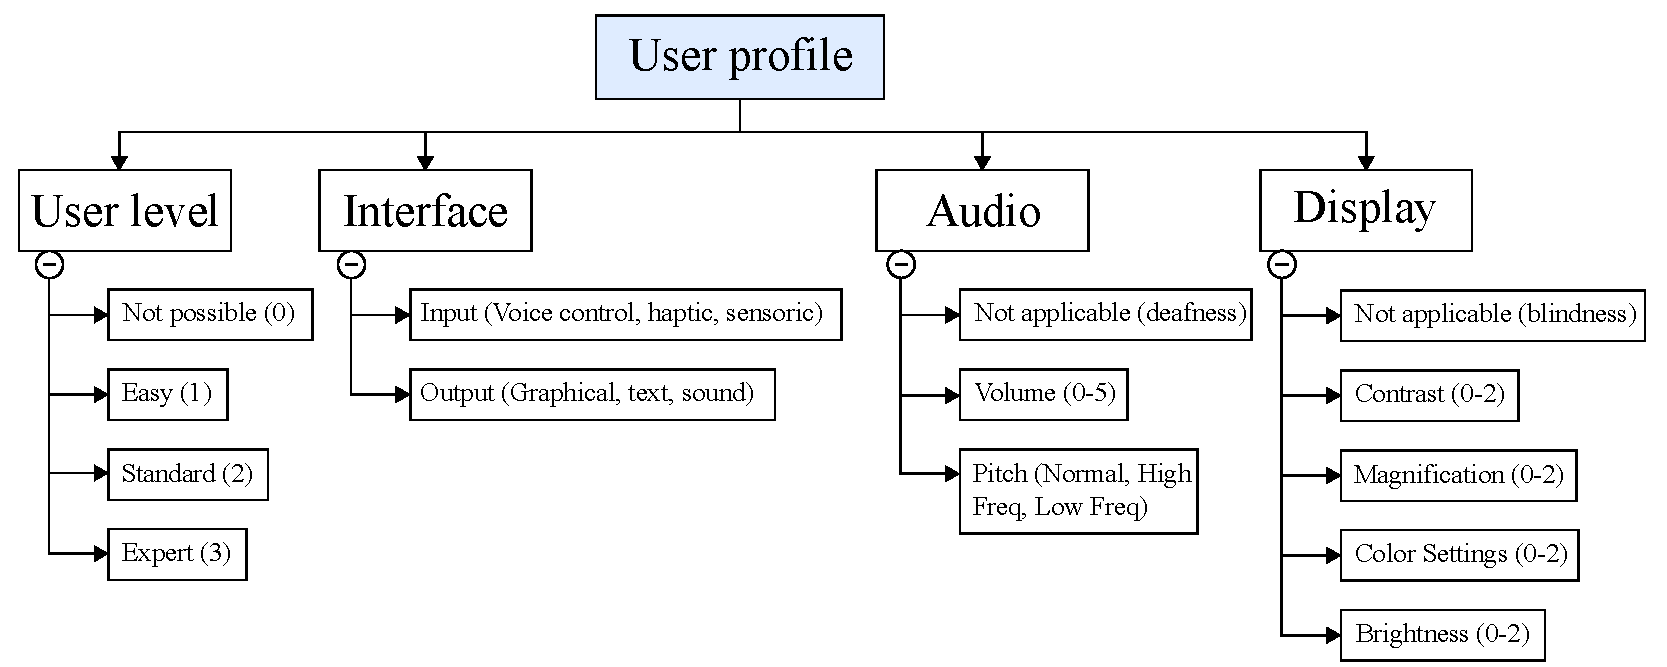
\includegraphics[width=1.0\textwidth]{../figures/PDF/casas.pdf}
\caption{User profile taxonomy by~\citet{casas_user_2008}.}
\label{fig:casas}
\end{figure}

AdaptUIOnt is built under this idea, extending it and avoiding the modelling of
any explicit physiological characteristics. As it will be depicted in this chapter
several concepts changed in our proposal. Besides, several remarkable ontologies
from other authors are also used to enrich the AdaptUIOnt knowledge. For example,
the \ac{foaf} ontology~\citep{foaf} has been linked to complete the information 
of the user. The same happens with the \ac{gumo}~\citep{heckmann_gumogeneral_2005}, 
which also models information about the user. Although not all classes are 
included, several have been imported in the final version of the AdaptUIOnt 
model, as they might represent significant concepts for other developers. 
For example, in the \ac{gumo} ontology there is a class which models the user 
emotional state (\textit{Basic User Dimensions} $\rightarrow$ 
\textit{Emotional State}) through five basic emotions. In  the current AdaptUIOnt 
version these emotions are not considered for the adaptations. However, we believe
that other developers may consider that being under an \textit{anxiety} condition
might change or modify the result or the adaptation process. Every ontology that
has been used to complete the AdaptUIOnt ontology is shown in Table~\ref{tbl:used_ontologies}.

\begin{table}[H]
  \caption{Imported ontologies to complete several concepts of the AdaptUIOnt
  ontology: \ac{gumo}, \ac{foaf} and \ac{cobra}.}
 \label{tbl:used_ontologies}
\footnotesize
\centering
 \begin{tabular}{l l l l}
  \hline 
  \textbf{Ontology} 		& \textbf{Class}		& \textbf{Description}		& \textbf{Imported subclasses}		\\
  \hline
  \ac{gumo}~\citep{heckmann_gumogeneral_2005}& \textit{Basic User Dimensions}& It originally models 	& \textit{Ability And Proficiency},\\
				& 				& different aspects of 		& \textit{Characteristics},		\\
				& 				& the user, as certain 		& \textit{Contact Information},		\\
				&				& abilities, emotional 		& \textit{Demographics},		\\
				&				& status, and so on.		& \textit{Motion}, \textit{Role},	\\
  				& 				&  				& \textit{Emotional State},		\\
  				& 				&  				& \textit{Personality}, \textit{Mental}	\\
  				& 				&  				& \textit{State}, \textit{Physiological}\\
  				& 				&  				& \textit{State}			\\
  				& \textit{Context Information}	& It represents several		& \textit{Location} and \textit{Physical}\\
  				&				& concepts related to 		& \textit{Environment} and \textit{Social}\\
  				&				& the environment.		& \textit{Environment}.			\\
  \ac{foaf}~\citep{foaf}	& \textit{Document}		&  	 			& \textit{Image} and 			\\  
				& 				&				& \textit{PersonalProfileDocument}.	\\
				& \textit{SocialInstitution}	& 				& 					\\
				& \textit{OnlineAccount}	& 				& \textit{Online Chat Account},		\\
				& 				&				& \textit{Online E-commerce} 		\\
				& 				&				& \textit{Account} and \textit{Online} 	\\
				& 				&				& \textit{Gaming Account}.		\\
  \ac{cobra}~\citep{cobra}	& \textit{DeviceMemory}		& 				& 					\\
				& \textit{DisplayScreen}	& 				& 					\\
				& \textit{DisplayScreenResolution}& 				& 					\\
				& \textit{MemoryUsageType}	& 				& 					\\
  \hline
  
\end{tabular}
\end{table}


Other works have also been taken into account for the user model. For example
~\citet{gregor_designing_2002} consider that users (in this case, the elderly)
evolve and their capabilities might change not just because of their experience
but because of the context influence. For Gregor et al. elderly's capabilities
decrease due to their ageing. In this dissertation, this evolution of the user
capabilities is considered to be based on the context conditions and experience.
This is explained in Section~\ref{sec:adaptation_polisher}, in which a concrete
module of the AdaptUI architecture is introduced.

Through the AdaptUIOnt's user model we also aim to allow users to configure
the adaptation process through the cited perspective, which is, without any required
physiological knowledge. During this configuration the user interacts with a
module called Capabilities Collector indicating several interaction requirements.
This module translates the user indications into a capabilities module. The
Capabilities Collector and all its features are detailed in
Section~\ref{sec:capabilities_collector}.

Regarding the context, several considerations were also discussed during the design
process. Context is mainly defined by its physiological conditions. Besides,
the \ac{gumo}~\citep{heckmann_gumogeneral_2005} ontology has been used to enrich the
model. The context model is extended in two different ways: on the one hand,
there is the sensors information and the combination of their measures (environment
data); on the other hand, a high-level information category built from the
combination of context and external pieces of information.

Devices are also modelled using different \ac{cobra}~\citep{cobra} classes. These
classes represent static and dynamic concepts of the device. Device's screen
resolution (\textit{DisplayScreenResolution}) is one of the static features of a
mobile device. On the contrary, the battery of the device changes with the use.
This is represented through the \textit{Battery} class, and is also used by
AdaptUIOnt to represent this concept. AdaptUIOnt remarks the dynamic characteristics
of these devices, which are usually not modelled and are vital for the result of
any kind of adaptation. Thus, several classes representing dynamic characteristics
of mobile devices are added.



\subsection{Designing the AdaptUIOnt Ontology}
\label{sec:model_detail}

The AdaptUIOnt ontology has been designed with two main considerations in mind.
First, taking into account that useful and practical (and non physiological)
capabilities of the user, context and device need to be represented in the model.
This is carried out by reviewing the literature models and making several
adaptations, modifications and contributions. For example, regarding the user
model, we use \ac{foaf}~\citep{foaf} and \ac{gumo}~\citep{heckmann_gumogeneral_2005} to
model the user most personal characteristics. Nevertheless, the user model is
not based on these ontologies. It is built under several assumptions made by
\citet{casas_user_2008} in their user profile taxonomy, with several modifications.
Regarding the three entities, the ontology understands each one as a set of
characteristics that define them. Thus, there is, for example, a \textit{User}
class with a relationship \textit{definedBy} which relates the concept of a user
with the characteristics that define him/her (the \textit{UserCharacteristics}
class). The same conceptualization is shared by the other two entities (see
Figure~\ref{fig:entities_characteristics}). This part of the ontology has been
called \textit{Entities Model}, and it is detailed in Section~\ref{sec:entities_model}.



\begin{figure}
\centering
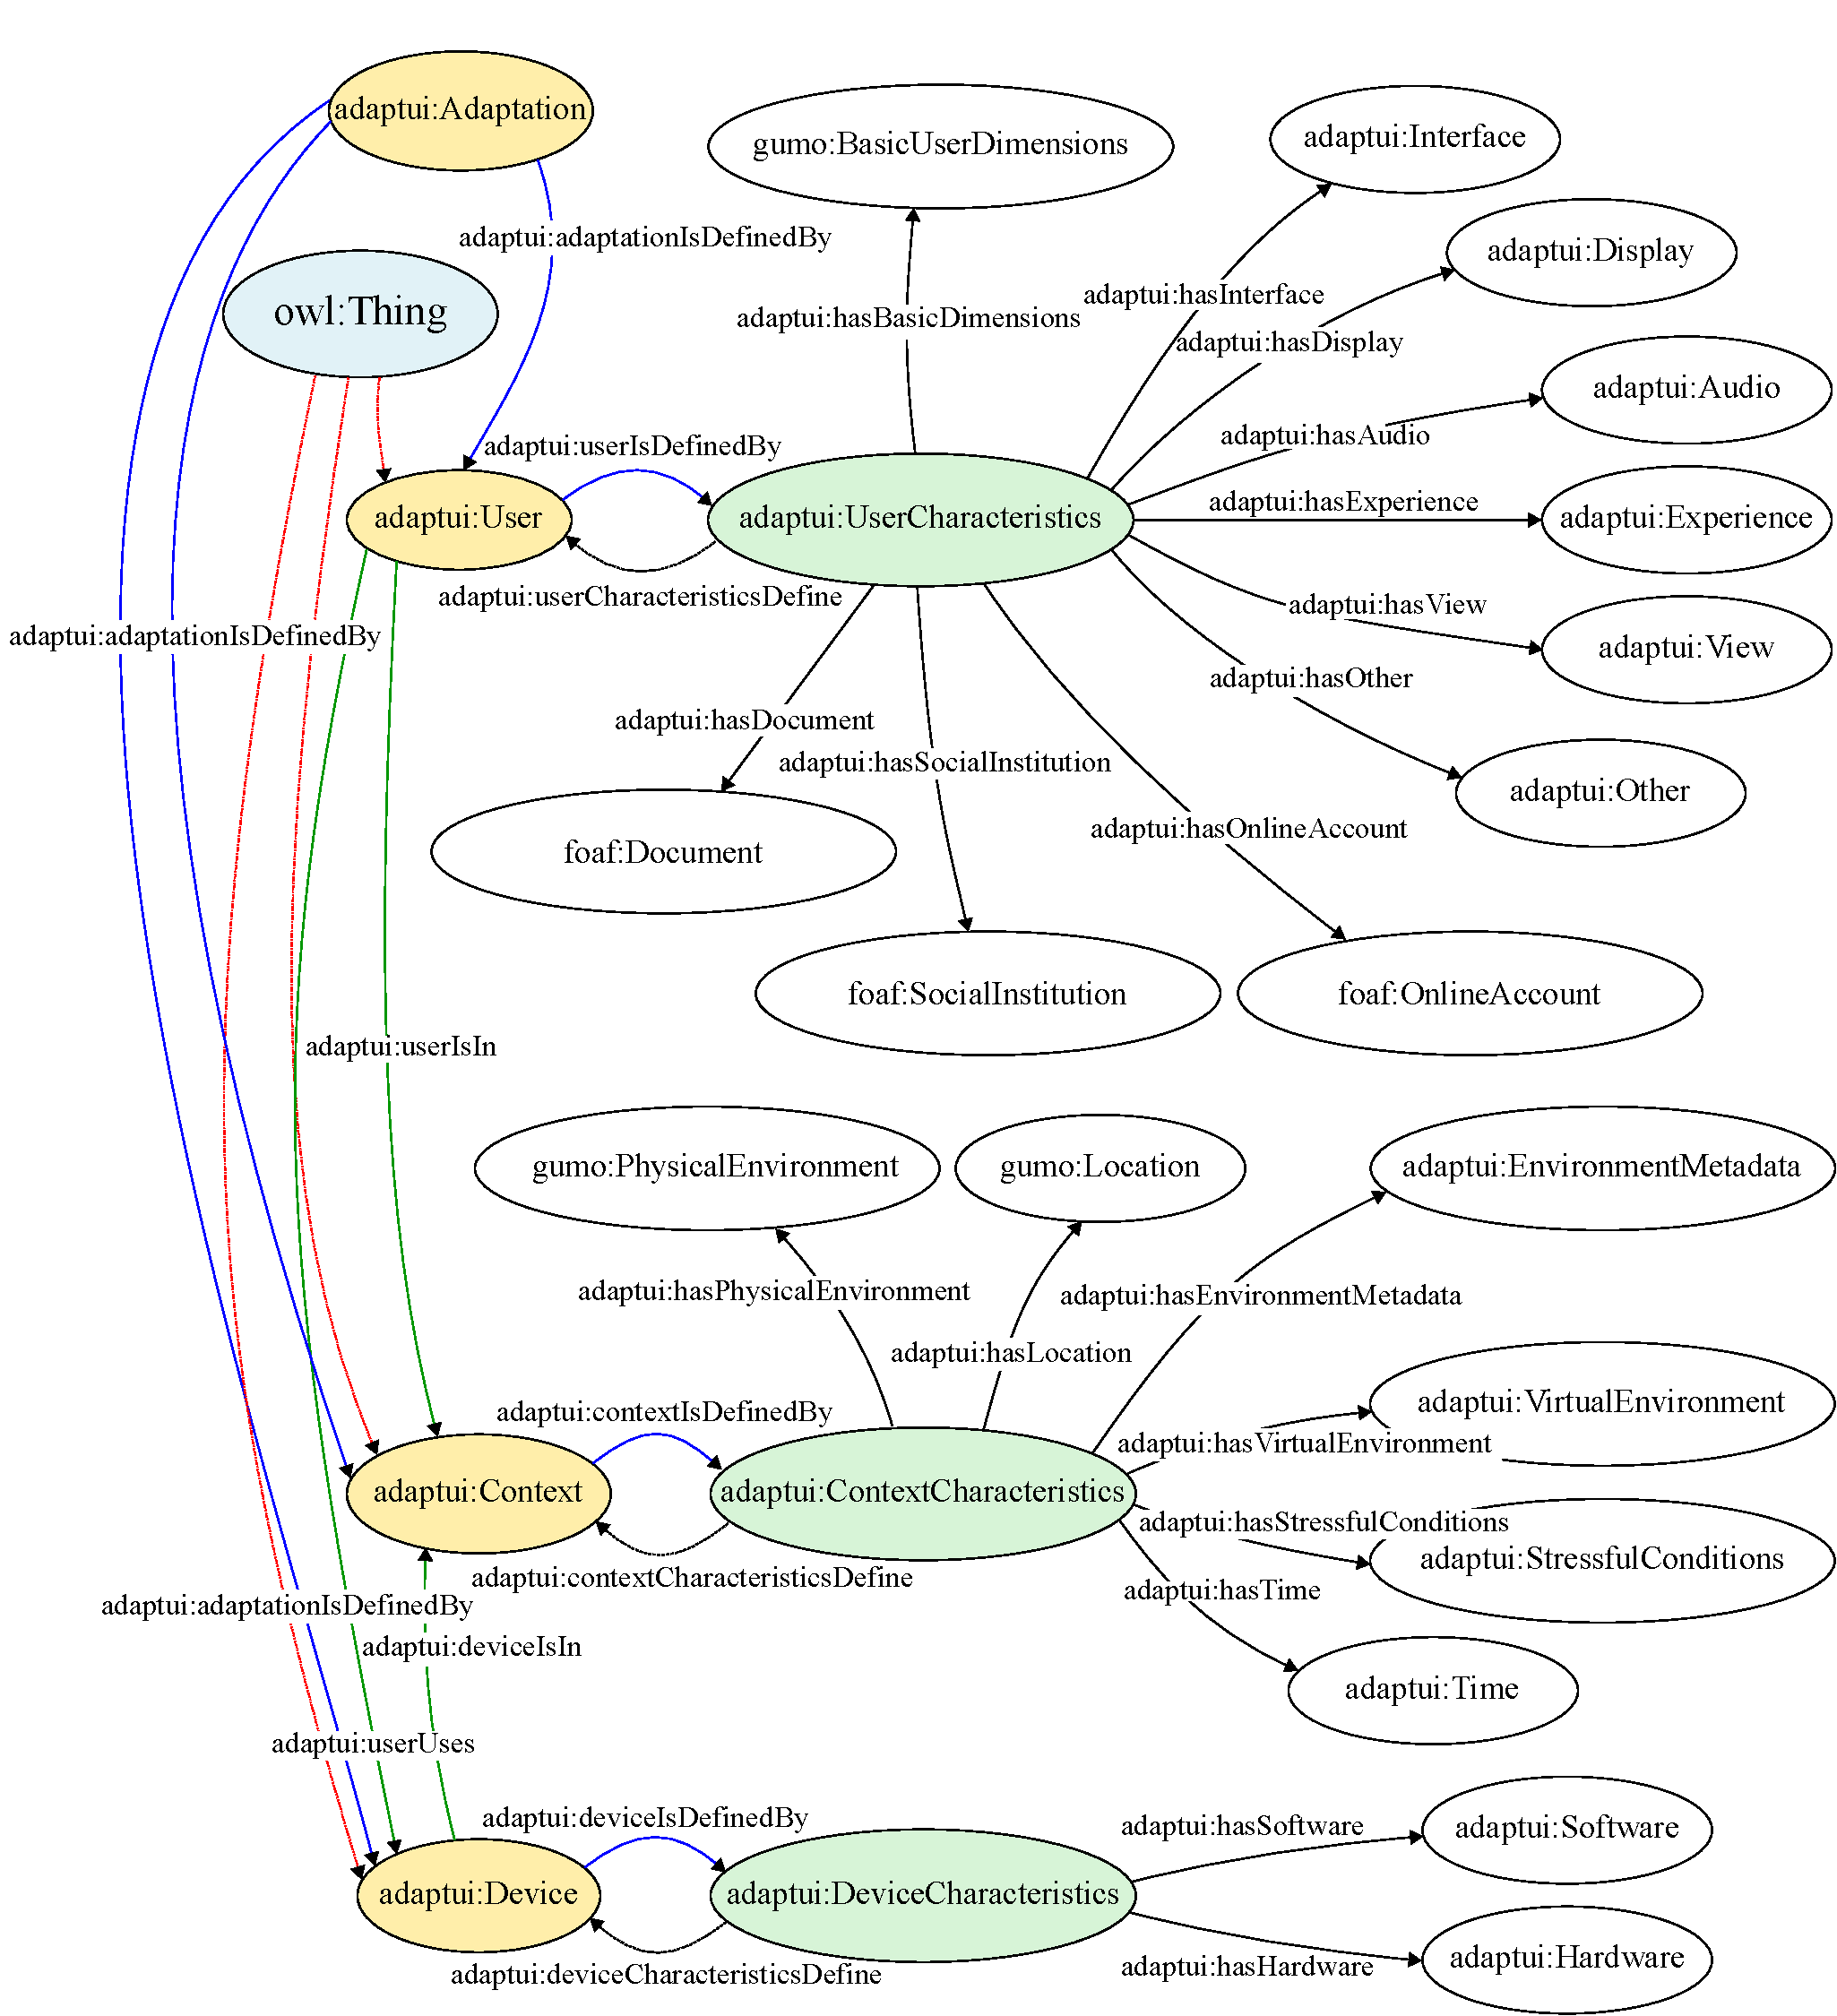
\includegraphics[width=0.90\textwidth]{../figures/PDF/entities_characteristics}
\caption{\textit{User},
\textit{Context} and \textit{Device} classes (in yellow) and their main object
relationships. As is shown, these classes are defined by their corresponding
characteristics class (in green).}
\label{fig:entities_characteristics}
\end{figure}


Second, and based on the conclusions made by~\citet{gregor_designing_2002},
the proposed ontology aims to be aware of the possible dynamic variations of the
environment, which may affect to the three entities. Therefore, we have implemented
several auxiliary classes to collect all the temporary knowledge within the
environment. These classes, shown in Figure~\ref{fig:auxiliary_classes}, are
linked to the main classes and complete them through several triggered rules
(see Section~\ref{sec:adaptui_rules}). This part of the dynamic knowledge
representation of the AdaptUIOnt ontology has been called \textit{Dynamic Model},
and it is explained in Section~\ref{sec:dynamic_model}.


\begin{figure}
\centering
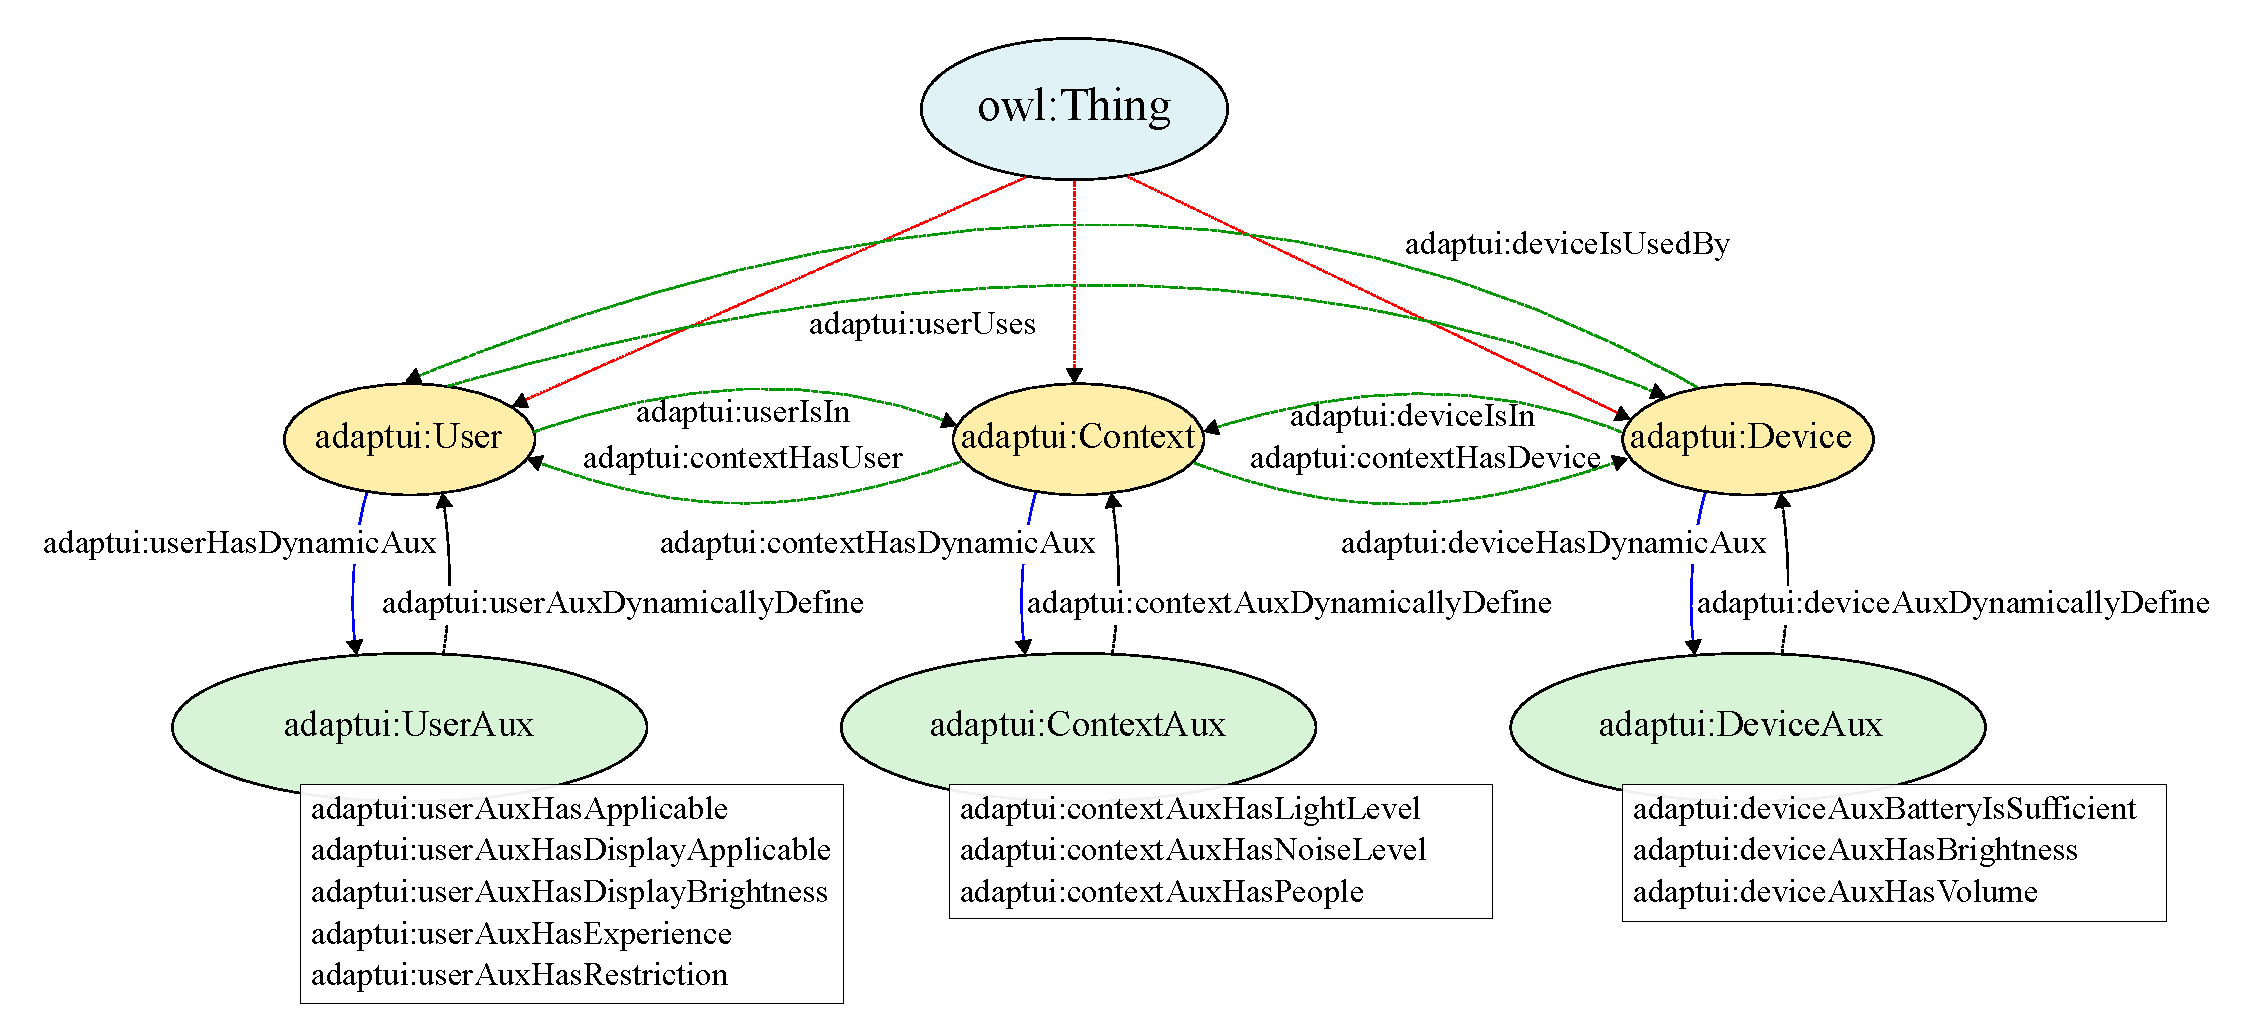
\includegraphics[width=1.0\textwidth]{../figures/PDF/auxiliary_classes.pdf}
\caption{\textit{UserAux}, \textit{ContextAux} and \textit{DeviceAux} classes
(in yellow) and their main datatype relationships.}
\label{fig:auxiliary_classes}
\end{figure}

As said before, AdaptUI allows users to manage the adaptation model through the
Capabilities Collector module. This idea, based on the work by~\citet{razmerita_ontology_based_2003},
allows users to participate during the model personalization and adaptation process. 
To this end, several classes have an \textit{isStatic} data property. This property
enables or disables the adaptation for the corresponding class depending on its
value (\textit{true} or \textit{false}). For example, the user might not want the
display brightness to be changed. A user profile where the brightness is configured
as static with the corresponding boolean value (\textit{adaptui:userdisplayBrightnessIsStatic})
means that during the adaptation process the corresponding rule (see the adaptation
rules set in Section~\ref{sec:adaptui_rules}) will evaluate this property
and finally avoid any change for the brightness parameter. The set of AdaptUIOnt
classes, object and datatype properties are shown through Figure~\ref{fig:classes},
Figure~\ref{fig:object_properties} and Figure~\ref{fig:datatype_properties}
respectively.

%CLASSES
\begin{figure}
\centering
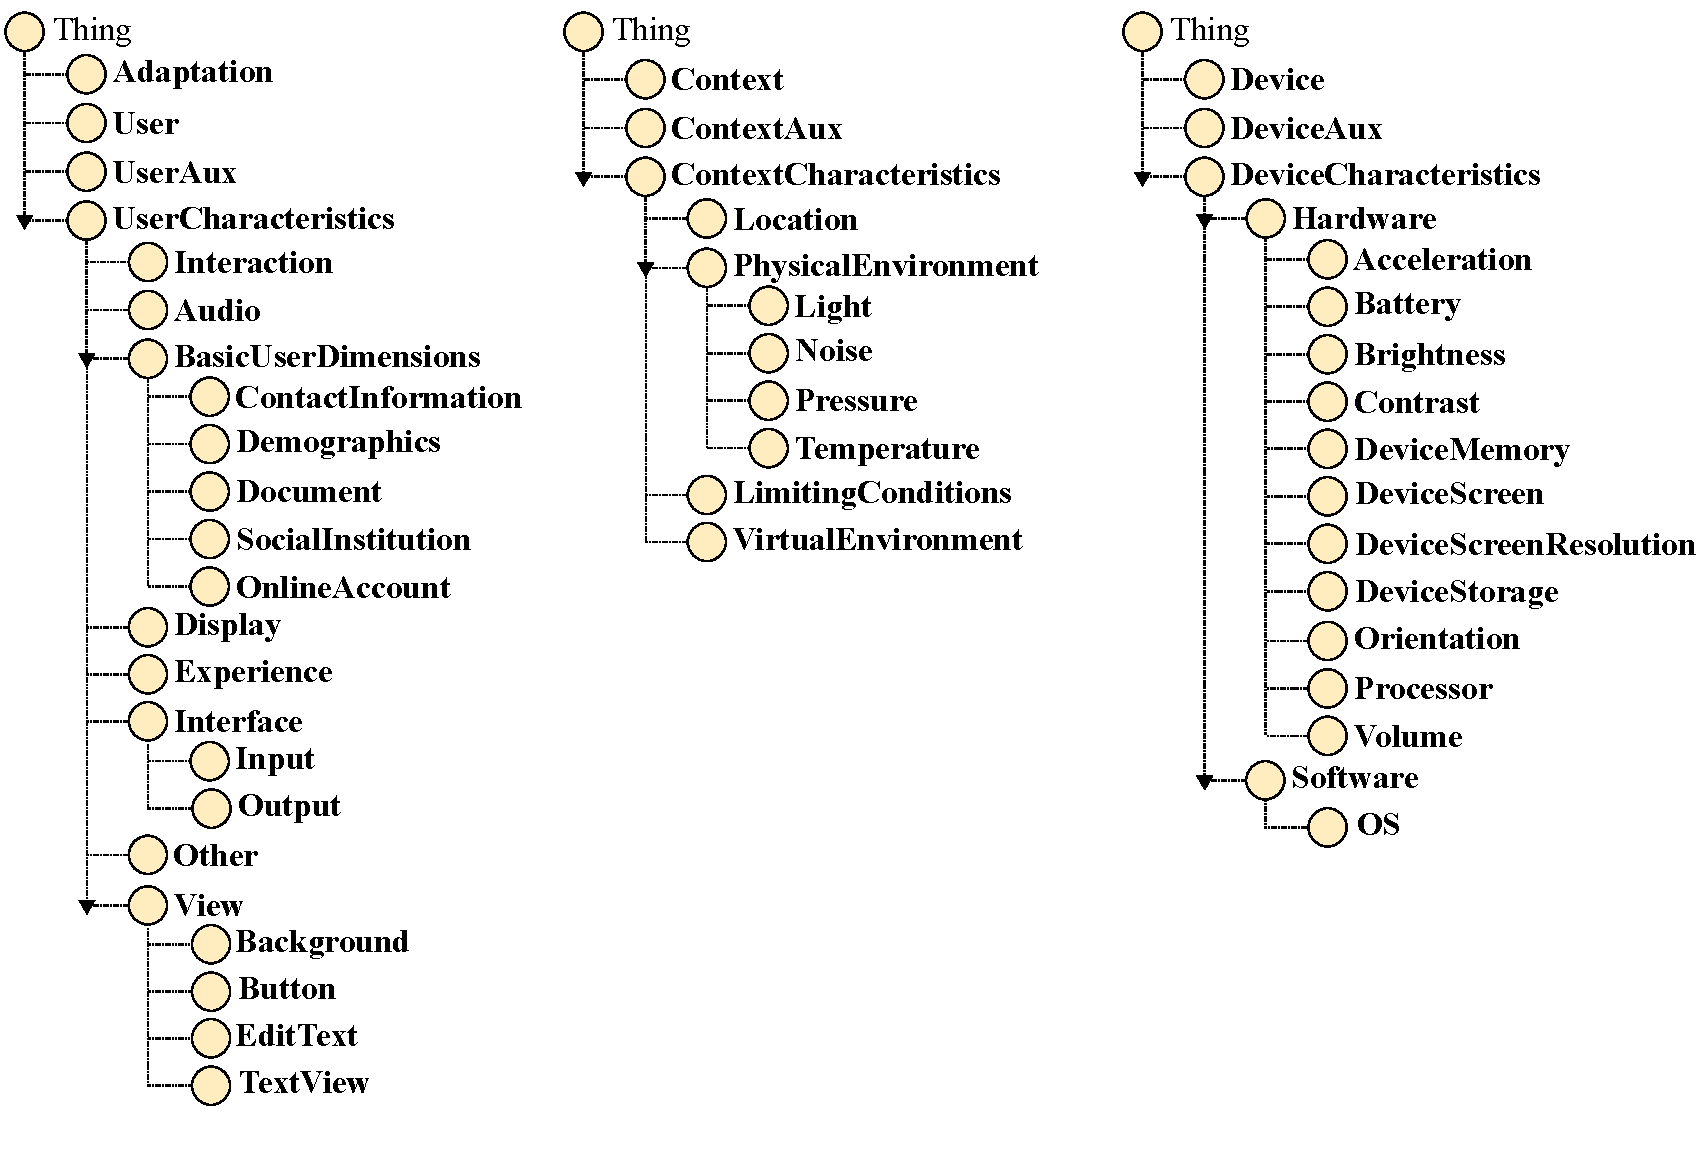
\includegraphics[width=0.95\textwidth]{../figures/PDF/classes.pdf}
\caption{\textit{User} (left), \textit{Context} (centre)
and \textit{Device} (right) classes of the AdaptUI ontology.}
\label{fig:classes}
\end{figure}

%OBJECT PROPERTIES
\begin{figure}
\centering
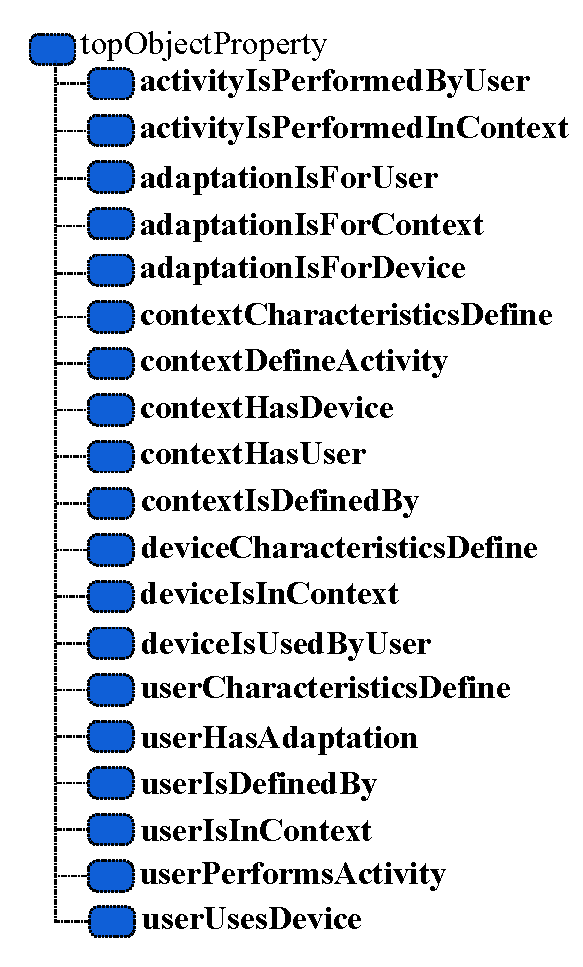
\includegraphics[width=0.33\textwidth]{../figures/PDF/object_properties.pdf}
\caption{AdaptUI object properties.}
\label{fig:object_properties}
\end{figure}

%DATATYPE PROPERTIES
\begin{figure}
\centering
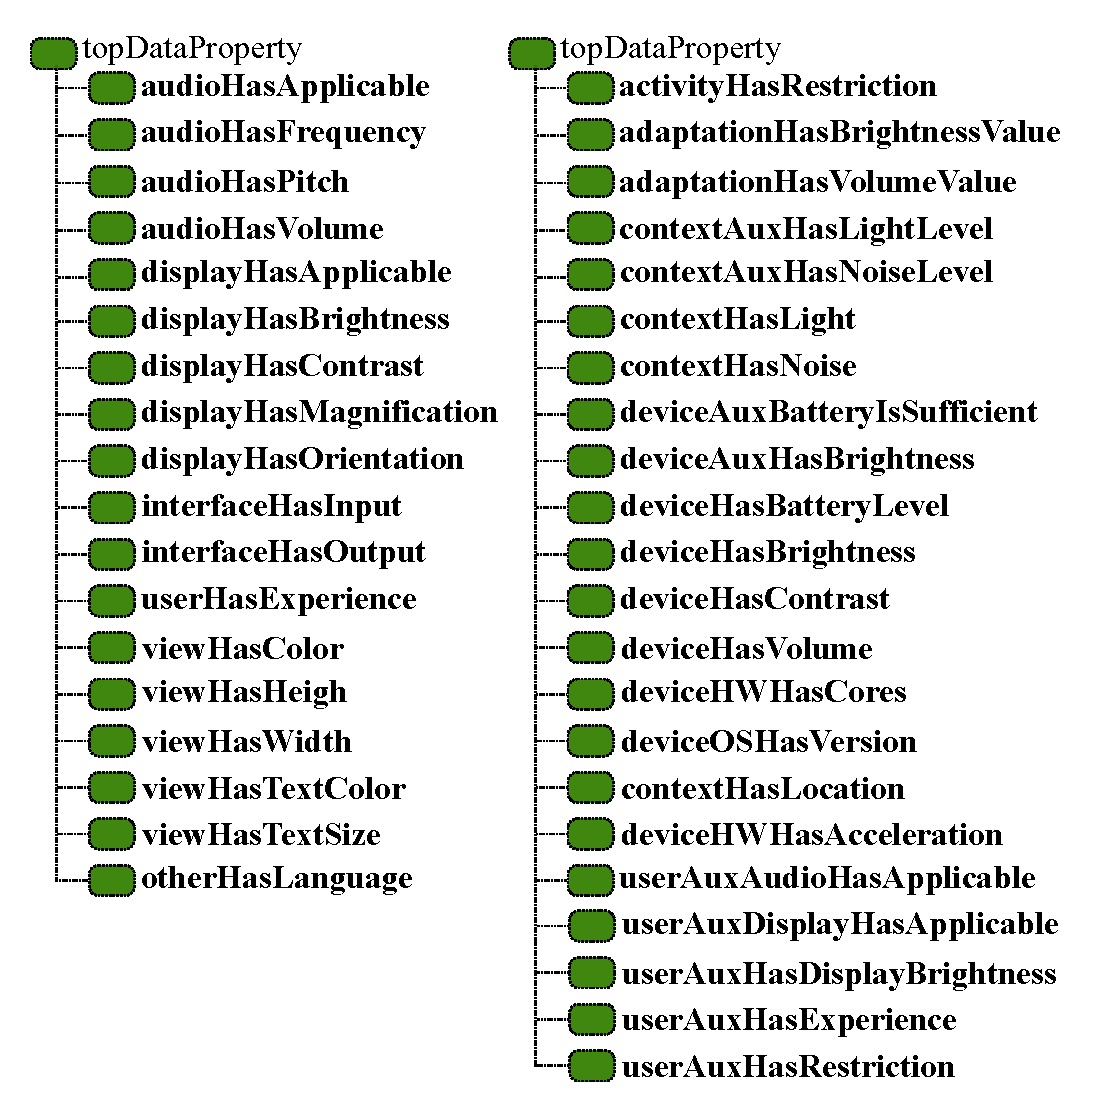
\includegraphics[width=0.65\textwidth]{../figures/PDF/datatype_properties.pdf}
\caption{AdaptUI datatype properties, not considering other ontologies. The left
group of properties are those related to
the \textit{UserCharacteristics} class.}
\label{fig:datatype_properties}
\end{figure}


\subsection{The \textit{Entities Model}}
\label{sec:entities_model}

After reviewing the literature in Chapter~\ref{cha:state_of_the_art} we found
that, for an appropriate adaptation of a user interface, there are three main
entities which must be represented in the domain: the user, the context and the
device. These concepts are semantically represented through the \textit{User},
\textit{Context} and \textit{Device} classes in the AdaptUIOnt ontology. But 
these three classes do not represent these entities alone. They are defined by 
their corresponding characteristics. These characteristics are represented through 
the \textit{UserCharacteristics}, \textit{ContextCharacteristics} and
\textit{DeviceCharacteristics} classes (see Figure~\ref{fig:user_characteristics_class}).
Together with the \textit{Adaptation} class, these seven classes form the Entities
Model, which is a conceptual group within the whole AdaptUIOnt model.
Figure~\ref{fig:entities_characteristics} shows the set of classes which form
the Entities Model.

\begin{figure}
\centering
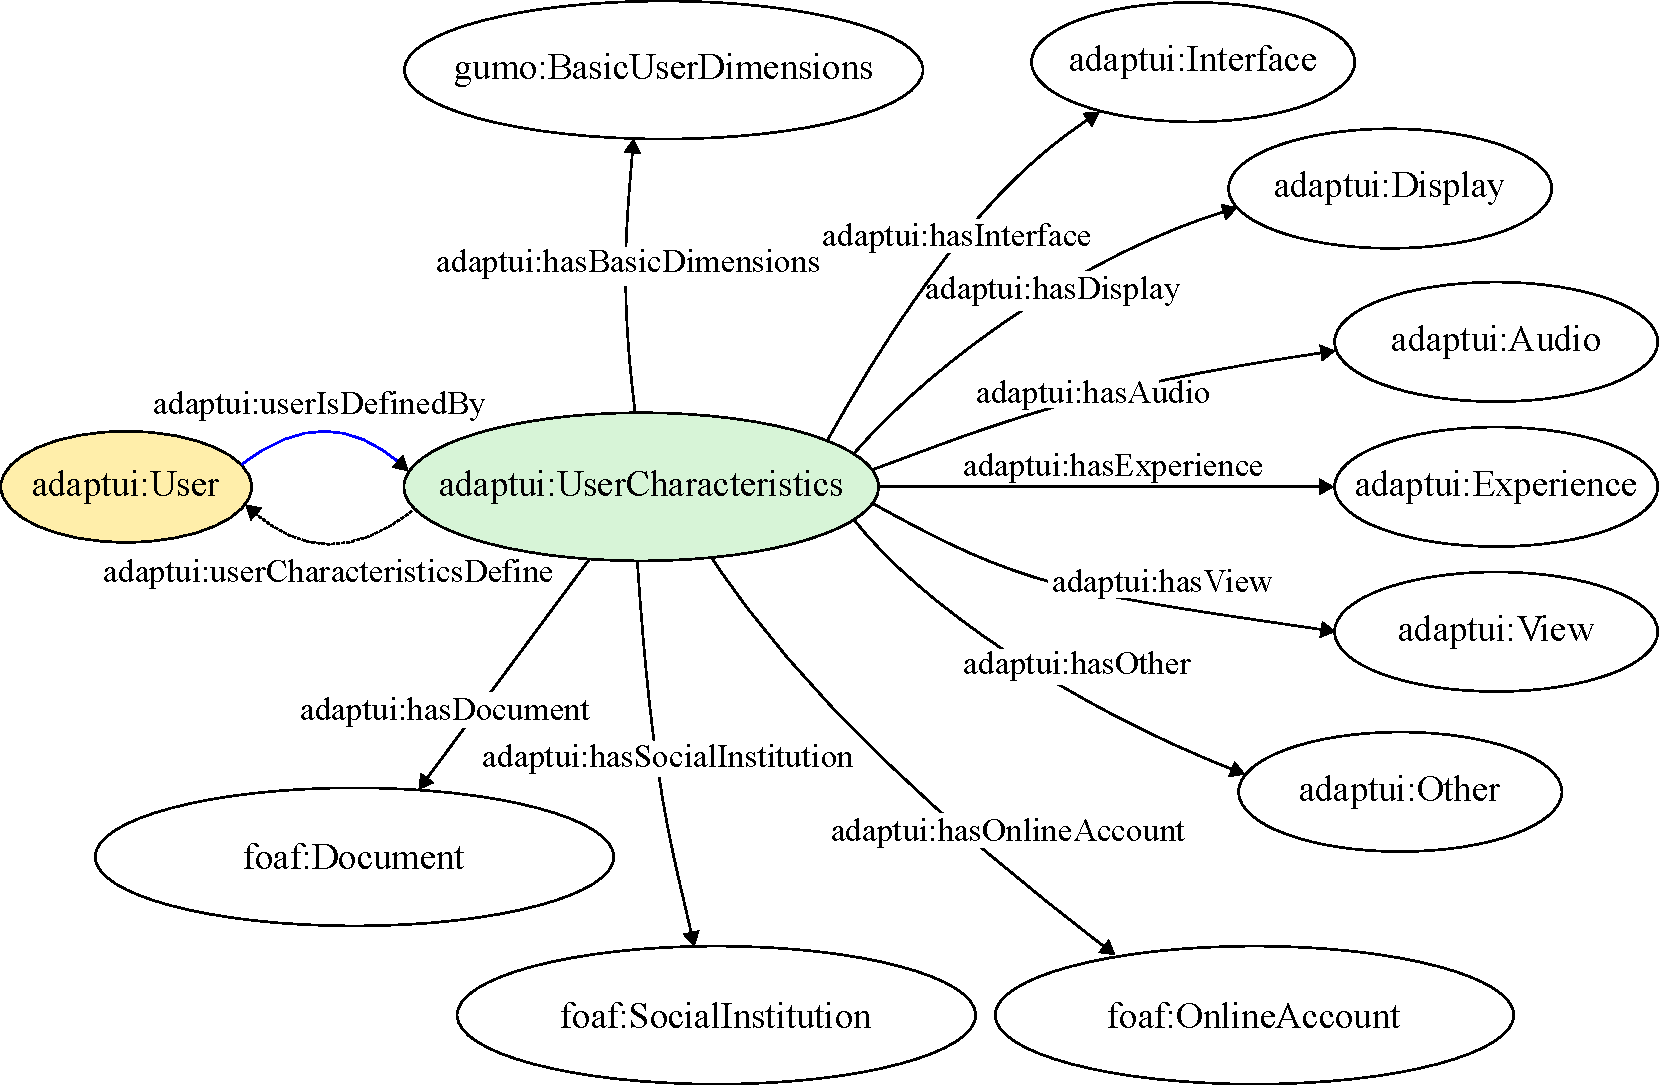
\includegraphics[width=0.85\textwidth]{../figures/PDF/user_characteristics_class.pdf}
\caption{The \textit{User} and the \textit{UserCharacteristics} classes.}
\label{fig:user_characteristics_class}
\end{figure}

Through the following sections the classes which belong to the Entities Model
are detailed. First, the \textit{UserCharacteristics} class is described in
Section~\ref{sec:user_characteristics_class}. Next, the \textit{ContextCharacteristics}
class is detailed (see Section~\ref{sec:context_characteristics_class}). Third,
a description of the \textit{DeviceCharacteristics} class is given in
Section~\ref{sec:device_characteristics_class}. Finally, the \textit{Adaptation}
class is detailed in Section~\ref{sec:adaptation_class}.


\subsubsection{The \textit{UserCharacteristics} Class}
\label{sec:user_characteristics_class}

The \textit{UserCharacteristics} class is one of the seven classes included in
the conceptual Entities Model. This class includes a series of subclasses which
build the knowledge about the user. Several user modelling ontologies are used
(i.e., \ac{foaf}~\citep{foaf} and \ac{gumo}~\citep{heckmann_gumogeneral_2005}). 
However, the strength of this class lies not on the representable knowledge 
through these classes, but in the way the knowledge about the user capabilities
(and disabilities) is represented. As explained in the introduction of this 
chapter, modelling physiological capabilities of users is troublesome and not 
practical. Several authors have tried to model user physiological characteristics~\citep{gregor_designing_2002}
\citep{razmerita_ontology_based_2003}~\citep{pereira_triple_2005}~\citep{persad_characterising_2007}
\citep{persad_cognitive_2007} and~\citep{skillen2012ontological}. Although their
systems may behave properly, there is still the issue of facing a coherent user
modelling process including user's capabilities. Not only because we lack
physiological background in the area, but also because different users may behave
in different ways even if they suffer from the same disability. 

To avoid this problem and to provide an ontology able to model user's 
capabilities, AdaptUIOnt's user's capabilities and disabilities knowledge is 
represented through the following classes:

\begin{itemize}
  \item \textit{Interface}: This category gathers input and output information
  about the user interaction preferences. Instead of modelling physiological
  capabilities regarding user's interaction abilities (e.g., sight capabilities),
  the model focuses in taking into account the user needs. For example, a user
  with a sight problem will not have to model a specific sight disability. This
  would require to consider several sight conditions and, for each one, different
  measures, ranges and classifications. Instead of that, there is the possibility
  for the user to model the Input/Output as voice and audio based interaction
  (by default the interaction is established as \textit{haptic}). This means that,
  by specifying these parameters, the system will understand that the user might
  suffer from a hearing loss condition or a sight disability.
  Table~\ref{tbl:user_characteristics_ontology} shows the interaction channels
  modelled by default in AdaptUIOnt.

  \item \textit{Audio} and \textit{Display}: These two classes model aspects
  about the use of the audio commands and volume controls, as well as different
  presentation parameters for the display, as brightness, contrast, orientation
  and magnification (see all the properties in Table~\ref{tbl:user_characteristics_ontology}).
  Thus, sight disabilities or, simply, sight problems due to context conditions
  (e.g., direct sunlight on the device screen) and hearing problems are faced by
  allowing the user to establish the default (or minimum) brightness, magnification,
  contrast, pitch, frequency and volume of the adaptation.
    
  \item \textit{Experience}: User experience with technology might be useful when
  executing adaptation rules. For examples, inexperienced users may need more
  instructions to run the profile (model) configuration process to add the
  corresponding knowledge about their capabilities.
  
  \item \textit{Other}: Several extra parameters (for example, the property
  \textit{has\_TTS}, which means that the user needs a tool which reads the text from
  the display). It also includes language and vibration related aspects.
  
  \item \textit{View}: User interfaces are composed of different views (\acs{gui} 
  elements) that are combined for representing different applications and services. 
  For each of these views (e.g., a button) the model considers several properties 
  that the user can configure (i.e., size and colours). For example, users with 
  colour blindness can change the colours of the components before any adaptation 
  to specify the set of colours they are able to distinguish, or adjust a 
  minimum size for a button so the user is able to interact with it. Thus, in 
  the future adaptations, the adaptation rules will be aware of this user 
  particular need.
  
  \item \textit{Basic User Dimensions}: Extracted from the \ac{gumo} ontology
  \citep{heckmann_gumogeneral_2005}, this class models information about the user
  contact information. See Table~\ref{tbl:used_ontologies} in order to see the
  whole set of classes included under this class.
  
  \item \textit{Document}, \textit{SocialInstitution} and \textit{OnlineAccount}:
  Extracted from \ac{foaf}~\citep{foaf}, these classes complete several personal 
  and social characteristics of the user.
\end{itemize}



\begin{center}
\footnotesize
\begin{longtable}{l l l}
  
  \label{tbl:user_characteristics_ontology} \\
  \hline 
  \textbf{Subclass} 	& \textbf{Property name} 	& \textbf{Description}							\\
  \hline
  \textit{Interface}	& \textit{interfaceHasInput}	& This property models the possible input methods for the		\\
			& 				& user with the following possibilities: \textit{gestures}, \textit{haptic},\\
			& 				& \textit{voice\_control}, \textit{sensory}, \textit{only\_haptic}, \textit{only\_voice\_control}.\\
			& \textit{interfaceHasLanguage}	& Describes to define the desired language. 				\\
			& \textit{interfaceHasOutput}	& This property models the possible output  methods for 		\\
			& 				& the user with the following possibilities: \textit{standard}  	\\
			& 				& (images, text, video and sound), \textit{only\_audio}, \textit{only\_text}.	\\
  
  \textit{Audio}	& \textit{audioHasApplicable}	& Describes if audio interaction is applicable for the user. 		\\ 
			& 				& If \textit{false}, we infer that the user might suffer from		\\
  			& 				& some hearing problems.						\\
  			& \textit{audioHasFrequency}	& Represents the preferred audio frequency. 				\\
  			& \textit{audioHasPitch}	& Describes the preferred pitch. 					\\
  			& \textit{audioHasVolume}	& Represents value which points out the desired audio 			\\
  			&				& volume.								\\
  			
  \textit{Display}	& \textit{displayHasApplicable}	& Describes the capability of the user to interact with			\\
			& 				& the display. If \textit{false} we might understand that the user 	\\
			& 				& suffers from a sight disability.		 			\\
			& \textit{displayHasBrightness}	& Represents value representing the brightness value.			\\
			& \textit{displayHasContrast}	& Describes indicating the contrast value.				\\
			& \textit{displayHasMagnification}& Represents value which represents the magnification			\\ 
			&				& degree needed for the user to properly see the display.		\\
			& \textit{displayHasOrientation}& Describes two options: \textit{landscape} or \textit{portrait}.  	\\
			& 				& This parameter indicates the preferred display 	 		\\
			&				& orientation for the user.						\\
  
  \textit{Experience}	& \textit{userHasExperience}	& A set of possible values to describe user's experience 		\\
			& 				& qith technology: \textit{standard}, \textit{advanced}, \textit{not\_applicable}.\\
  
  \textit{View}		& \textit{viewHasColor}		& Describes the colour for the view background.				\\
			& \textit{viewHasWidth}		& Represents value to determine the width of the view.			\\
			& \textit{viewHasHeight}	& Describes the height of the view.					\\
			& \textit{viewHasTextColor}	& Represents value representing the colour for the text.		\\
			& \textit{viewHasTextSize}	& Represents value representing the text size.				\\
  \hline 
\caption{UserCharacteristics data properties}
\end{longtable}
\end{center}


\subsubsection{The \textit{ContextCharacteristics} Class}
\label{sec:context_characteristics_class}

Usually, context is modelled considering that the data collected by sensors is
enough to characterize it. In AdaptUIOnt this kind of context is also modelled,
since sensor information is significantly relevant for being aware of the context
environment conditions. Thus, the information collected by sensors is represented
under the \textit{PhysicalEnvironment} and \textit{Location} classes, which are
classes from the \ac{gumo}~\citep{heckmann_gumogeneral_2005} ontology. Nevertheless,
the AdaptUIOnt ontology does not only model sensor related knowledge. There are
three extra classes which aim modelling high-level information about the
environment: \textit{LimitingConditions}, \textit{VirtualEnvironment} and
\textit{EnvironmentMetadata}. In the following lines a description of each class
is presented:

\begin{itemize}
 \item \textit{PhysicalEnvironment}: Environment information collected from
 sensors (e.g., absolute location, available resources, light and noise conditions).
 
 \item \textit{Time} and \textit{Location}: Both classes are used to characterize
 each user and device in a temporal and location context. Both entities are linked
 to these context variables through the \textit{userIsIn} and \textit{deviceIsIn}
 object properties (see Figure~\ref{fig:object_properties}).
 
 \item \textit{LimitingConditions}: Instead of modelling a set of particular
 activities we consider several context situations that might impede the interaction
 with the user. These situations are modelled as different groups regarding the
 capabilities that they might affect.
 
 \item \textit{VirtualEnvironment}: Combining the knowledge of the categories
 above, it is possible to extract high-level information. For example, sensing
 that there is a light at the office, it is possible to infer that there are
 people working. Thus, we avoid the use of other sensors to indicate this
 activity.
 
 \item \textit{EnvironmentMetadata}: Environment knowledge is associated to
 sensors. A sensor can provide information about the temperature (23 ºC). But
 this information by itself is poor in a context-aware system. Environment metadata
 can describe and enrich this knowledge, providing time and location data. For
 example, ``the current temperature at 12:00 AM in Bilbao is 13 ºC''.
\end{itemize}


Table~\ref{tbl:context_characteristics_ontology} shows the main datatype properties
of the \textit{ContextCharacteristics} class.

\begin{table}[H]
  \caption{ContextCharacteristics data properties}
 \label{tbl:context_characteristics_ontology}
\footnotesize
\centering
 \begin{tabular}{l l l}
  \hline 
  \textbf{Subclass} 	& \textbf{Property name} 	& \textbf{Description}		\\
  \hline
  \textit{Location}	& \textit{hasRelativeLocation}	& Represents relative locations.\\
			& \textit{hasAbsoluteLocation}	& Describes \textit{longitude} and \textit{latitude}.\\
  \textit{Light}	& \textit{contextHasLight}	& Describes the amount of \ac{lx}\\
			& 				& in the environment.		\\
  \textit{Noise}	& \textit{contextHasNoise}	& Represents the amount of \acp{db}\\
			& 				& in the environment.		\\
  \textit{Time}		& \textit{hasTimeValue}		& The current time.		\\
  \textit{LimitingConditions}& \textit{hasMovementRestriction}&				\\
  \hline
  
\end{tabular}
\end{table}



\subsubsection{The \textit{DeviceCharacteristics} Class}
\label{sec:device_characteristics_class}

The device model is also built over several useful classes from other ontologies.
The most important characteristic of this class consists in modelling dynamic
information about the device regarding the adaptation. For example, low battery
levels might be considered risky by the AdaptUI system, as there is the possibility
that the device turns off during the process. Device capabilities are categorized
as follows:

\begin{itemize}
 \item \textit{Software}, which encompasses different software aspects of the
 device (i.e., the \ac{os} platform). 
 
 \item \textit{Hardware}, designed to model information about the current status
 of different capabilities (i.e., available battery and memory).
\end{itemize}


Table~\ref{tbl:device_characteristics_ontology} shows the main datatype properties
of the \textit{DeviceCharacteristics} class.


\begin{table}
  \caption{DeviceCharacteristics data properties.}
 \label{tbl:device_characteristics_ontology}
\footnotesize
\centering
 \begin{tabular}{l l l}
  \hline 
  \textbf{Subclass} 	& \textbf{Property name} 	& \textbf{Description}		\\
  \hline
  \textit{Brightness}	& \textit{deviceHasBrightness}	& Describes the current		\\
			& 				& device's brightness.		\\
  \textit{Contrast}	& \textit{deviceHasContrast}	& Represents the current 	\\
  			& 				& device's contrast.		\\
  \textit{Volume}	& \textit{deviceHasVolume}	& Describes the current		\\
   			& 				& device's volume.		\\
  \textit{Processor}	& \textit{deviceHasHWCores}	& Models the number 		\\
			& 				& of the device's cores.	\\
  \textit{OS}		& \textit{deviceOSHasVersion}	& Indicates the current		\\
			& 				& \ac{os} version.		\\
  \textit{Acceleration}	& \textit{deviceHasAcceleration}& Represents the current 	\\
			& 				& X, Y, Z acceleration.		\\
  \textit{DeviceScreen,	Processor,}& \textit{hasFactoryValue}& Maximum values for 	\\
\textit{Orientation, DeviceMemory,}& 			& the elements under the  	\\
\textit{Battery, DeviceScreenResolution,} & 		& Sub-class column.  		\\
\textit{DeviceStorage} 	& 				& 				\\
  \hline

\end{tabular}
\end{table}


\subsubsection{The \textit{Adaptation} Class}
\label{sec:adaptation_class}

The last class included in the Entities Model is the \textit{Adaptation} class.
This class represents the final stage of the whole adaptation process. This means
that, after the adaptation process the results will be represented through an
individual (or instance) of this class. Therefore, the AdaptUI platform will
semantically request the corresponding adaptation for the user interface to this
class. As can be seen in Figure~\ref{fig:entities_characteristics}, the
\textit{Adaptation} class is linked to the other classes of the Entities Model
(\textit{User}, \textit{Context} and \textit{User}) through the \textit{adaptationIsDefinedBy}
object property. Thus, future semantic requests are allowed searching for a
specific user capability, context situation or device characteristics.
Table~\ref{tbl:adaptation_properties} shows the datatype properties of the
\textit{Adaptation} class.


\begin{table}
  \caption{\textit{Adaptation} class datatype properties.}
 \label{tbl:adaptation_properties}
\footnotesize
\centering
 \begin{tabular}{l l}
  \hline 
  \textbf{Datatype property} 			& \textbf{Description}				\\
  \hline
  \textit{adaptationBrightnessHasValue}		& Describes the final brightness value to be 	\\
						& configured in the device. 			\\
  \textit{adaptationVolumeHasValue}		& Represents the final volume value to be 	\\
						& configured in the device. 			\\
  \textit{adaptationButtonHasSize}		& Describes the final size value for a button. 	\\
  \textit{adaptationButtonHasBackgroundColor}	& Represents the final background colour for 	\\
						& a button.					\\
  \textit{adaptationButtonHasTextSize}		& Describes the final text size for a button.	\\
  \textit{adaptationButtonHasTextColor}		& Represents the final text colour for a button.\\
  \textit{adaptationEditTextHasSize}		& Describes the final size value for a edit text.\\
  \textit{adaptationEditTextHasBackgroundColor}	& Represents the final background colour for 	\\ 
						& a edit text.					\\
  \textit{adaptationEditTextHasTextSize}	& Describes the final text size for a edit text.\\
  \textit{adaptationEditTextHasTextColor}	& Represents the final text colour for a edit text.\\
  \textit{adaptationTextViewHasSize}		& Describes the final size value for a text view.\\
  \textit{adaptationTextViewHasBackgroundColor}	& Represents the final background colour for 	\\
						& a text view.					\\
  \textit{adaptationTextViewHasTextSize}	& Represents the final text size for a text view.\\
  \textit{adaptationTextViewHasTextColor}	& Describes the final text colour for 		\\
						& a text view.		 			\\
  \hline
  
\end{tabular}
\end{table}


% \section*{}


\subsection{Incoherence and Activities}
\label{sec:incoherence}

During the design of the AdaptUI ontology we have considered how the three
main entities (user, context and device) interact with each other. Modelling
these entities and being aware of the interactions that occur among them help
us to deduce the best adaptation for the user in each case. However, there are
several situations where the adaptation process is not so obvious. These situations
are defined by the activities that are being carried out within the environment.

\citet{persad_characterising_2007}~\citep{persad_cognitive_2007}
consider that activities need to be taken into account. They describe Human
Factors and Ergonomic theory as four components: the user, the product, the context
and the activities over time that constitutes the interaction.
\citet{hong_context_aware_2009} classify context conflicts into several categories:

\begin{itemize}
 \item Sensing conflict: Not matching results from several physical data sources.
 
 \item Service resource conflict: The lack of resources in a service offering
 process may provoke several conflicts.
 
 \item User preference conflict: Users whose profiles or preferences are different
 but having the same context situation may also result in context conflict.
\end{itemize}

During the designing process of AdaptUI, we asked ourselves if it would be enough
to consider just the user and his/her capabilities within the current context.
Thus, several hypothetical scenarios were studied:

\begin{itemize}
 \item A user suffers from a visual impairment. This disability obstructs
 the user from seeing the application content properly. Then the adaptation
 will intercede to facilitate another interaction channel for the user, e.g.,
 by voice recognition and control. The problem is that there are situations
 in which a common adaptation from the system will not be appropriate.
 For example, if the user is in a place where silence is essential (i.e., a
 library, a hospital or in an exam), an audio interaction based communication
 could not be appropriate. 
 
 \item A user who sees perfectly well interacts with the application's
 default user interface. If we avoid a situation in which the user is driving
 a visual/touch based adaptation could put the user in risk, as he/she would
 need to look at the display and use his/her hands.
 
 \item Another user is at home, and he/she does not suffer from any severe
 disability. At 01:00 pm he/she starts cooking. The application requests
 user attention for several tasks. This situation might be risky if the adaptation
 requests the user attention while he/she has, for example, oil in the pot, or
 he/she is manipulating knives.
\end{itemize}

These examples show several situations where users are involved in tasks that
contradict the current context and user capabilities. Adaptation incoherence is
defined by several environment parameters that induce the platform to perform a
certain adaptation for the current conditions. However, the result of this
adaptation, although it can be aligned with the context characteristics, can be
incoherent.

Therefore, we need something more to characterize the current situation that
involves these three entities: activities. Activities help us to understand the
current user, context and device situation. In other words, it enriches the
environment information.

Requiring the use of the hands, being at a certain location (like a library, where
people has to be in silence), or demanding the user attention are several examples
of situations which may represent some risks that we have to take into account
when we face a context modelling problem. For example, driving or cooking restricts
user capabilities momentarily. Hence, we can state that these activities impede
the user. As is difficult to model every possible activity that the user performs,
in AdaptUI we present a class (\textit{LimitingConditions}) that models abstract
groups of activities:

\begin{itemize}
 \item Activities that limit the use of the hands.
 \item Activities that limit the use of the voice.
 \item Activities that limit the user sight capability.
 \item Activities that limit the user attention.
 \item Activities that limit the user movement.
 \item Combinations of these activities.
\end{itemize}

\subsection{The \textit{Dynamic Model}}
\label{sec:dynamic_model}

The proposed solution addresses several issues of several modelling approaches
found in the literature. Following the perspective of~\citet{fischer_user_2001}
we consider that the modelled entities are not static at all. They change through
time due to their interaction. To express this concept of \textit{dynamic model}
we have implemented several auxiliary classes:

\begin{itemize}
 \item \textit{UserAux}: This class is helpful when a certain context situation
 impedes a user capability. Updated by the pre-adaptation rules this class is used
 as intermediary between the \textit{Adaptation} class and the \textit{ContextAux}
 class, where the classification of the context collected information is modelled.
 As is shown in Table~\ref{tbl:aux_classes_data_properties}, it models several user
 dynamic capabilities.
 
 \item \textit{ContextAux}: Context is considered in a different way. As context
 information comes from sensors, we have to translate the different incoming data
 to a more descriptive language. Thus, if a value of 35,000 lux is collected (as
 a brightness value of the \textit{ContextCharacteristics} class) we modify the
 contextAuxHasLightLevel data property with the \textit{direct\_sunlight} value (see
 Table~\ref{tbl:aux_classes_data_properties}). Therefore, it is possible to work
 with more meaningful data. The same occurs with the contextAuxHasNoiseLevel
 data property. Table~\ref{tbl:luminance} and Table~\ref{tbl:sounds} show the
 different classifications for light and noise levels used for AdaptUI.
 
 \item \textit{DeviceAux}: Following the same approach, this class deals with the
 dynamic capabilities of the device.
\end{itemize}

Working with sensor data opens new fronts regarding the AdaptUI platform. For
example, fuzzy reasoning would help to refine the collected information. This
is discussed in the Future Work section (see Section~\ref{sec:future_work}).


\begin{center}
\footnotesize
\begin{longtable}{l l l}
  \label{tbl:aux_classes_data_properties} \\
  \hline 
  \textbf{Class} 	& \textbf{Property name} 		& \textbf{Description}					\\
  \hline
  \textit{UserAux}	& \textit{userAuxDIsplayHasApplicable}	& Models the applicability of display adaptations for	\\
			& 					& the user. There are two different scenarios: 1) in 	\\
			& 					& the first one, the user might suffer from a 	\\
			&					& disability that makes impossible for him/her to	\\
			&					& interact with a display. In this case \textit{Display}\\
			& 					& is not applicable for this user; 2) on the contrary,	\\
			& 					& the user can specify that he/she does not want the 	\\
			& 					& display to be adapted. In any case the value of this	\\
			&					& property will determine if the rules need to consider	\\	
			& 					& \textit{Display}.					\\
			& \textit{userAuxAudioHasApplicable}	& Similar to the previous property, this one has the	\\
			& 					& same effect for audio adaptations.			\\
			& \textit{userAuxHasDisplayBrightness}	& Depending on the value of the \textit{UserCharacteristics}:\\
			& 					& \textit{userDisplayBrightnessIsStatic} property, the 	\\
			&					& corresponding rule will update this value indicating 	\\
			& 					& if the brightness should be considered for the 	\\
			&					& adaptation process.					\\
			& \textit{userAuxHasExperience}		& Represents user's experience with technology: \textit{easy},\\
			& 					& \textit{expert}, \textit{not\_possible}, \textit{standard}.\\
			& \textit{userAuxHasRestriction}	& User's activities are considered for adaptation. 	\\
			&					& Hence, a Boolean value is modelled in this property 	\\
			& 					& to indicate so.					\\
  \textit{ContextAux}	& \textit{contextAuxHasLightLevel}	& Represents several light classifications: \textit{clear\_night},				\\
			& 					& \textit{dark\_overcast}, \textit{daylight}, \textit{direct\_sunlight}, \textit{living\_room}, \\
			& 					& \textit{moonless\_clear}, \textit{moonless\_overcast}, \textit{office\_hallway}, 		\\ 
			& 					& \textit{office\_lightning}, \textit{overcast\_day}, \textit{sunrise}, \textit{twilight}.	\\
			& \textit{contextAuxHasNoiseLevel}	& Represents several noise classifications:							\\
			&					& \textit{absolute\_threshold\_of\_hearing}, \textit{breathing}, 				\\
			& 					& \textit{building\_work}, \textit{conversation}, \textit{factory},  				\\ 
			& 					& \textit{gig}, \textit{jackhammer}, \textit{leaves\_murmuring}, \textit{library},  		\\
			&					& \textit{office},  \textit{traffic}, \textit{train}, \textit{truck}, \textit{whispering}.	\\
  \textit{DeviceAux}	& \textit{deviceAuxBatteryIsSufficient}	& Based in Table~\ref{tbl:batteries}, indicates whether the \\
  			& 					& adaptation should be performed considering the 	\\
  			&					& current battery level.				\\
  			& \textit{deviceAuxHasBrightness}	& Describes the current brightness level of the device's\\
  			& 					&  screen.						\\
  \hline
\caption{Auxiliary classes' data properties.}\\
\end{longtable}
\end{center}



\begin{table}
  \caption{Luminance provided under various conditions~\citep{luminance}.}
 \label{tbl:luminance}
\footnotesize
\centering
 \begin{tabular}{l l l}
  \hline 
  \textbf{Brightness} & \textbf{Surfaces illuminated by}		& \textbf{Ontology value}	\\
  \textbf{(measured) in \ac{lx}}&					&				\\
  \hline
  0.0001		& Moonless, overcast night sky (starlight)	& \textit{moonless\_overcast}	\\
  0.002 		& Moonless clear night sky with air-glow	& \textit{moonless\_clear}	\\
  0.27-1.0		& Full moon on a clear night			& \textit{full\_moon}		\\
  1.0-3.4		& Dark limit of civil twilight under a clear sky& \textit{twilight}		\\
  3.4-50		& Family living room lights			& \textit{living\_room}		\\
  50-80 		& Office building hallway/toilet lighting	& \textit{office\_hallway}	\\
  80-100		& Very dark overcast day			& \textit{dark\_overcast}	\\
  320-500		& Office lighting				& \textit{office\_lightning}	\\
  500-1,000		& Overcast day; typical TV studio lighting	& \textit{overcast}		\\
  1,000-25,000		& Full daylight (not direct sun)		& \textit{daylight}		\\
  25,000-130,000	& Direct sunlight (latter figure is 		& \textit{direct\_sunlight}	\\
			& above atmosphere)				& 				\\
  \hline

\end{tabular}
\end{table}


In order to describe the whole detailed model and how the main classes are related
to each other, Figure \ref{fig:flow_diagram} shows how the knowledge flows through
the AdaptUI platform. First, the three main classes of the \textit{Entities Model}
are populated with the information about the user, the context and the device.
Then, the pre-adaptation rules are triggered and updates classifies and updates
the collected knowledge into intermediate knowledge. This knowledge is represented
in the \textit{UserCharacteristics}, \textit{ContextCharacteristics} and
\textit{DeviceCharacteristics} classes. Finally, the \textit{Adaptation} class
requests the processed knowledge and through the adaptation rules the final
adaptation is sent to the user. Additionally, within the user model the interaction
model collects information about the interaction, updating the \textit{UserAux}
class if needed. This brings the execution of the rules again, which means that
a new result is generated.


\begin{table}[H]
  \caption{Most common sound intensity levels modelled by default in AdaptUI.}
 \label{tbl:sounds}
\footnotesize
\centering
 \begin{tabular}{l r}
  \hline 
  \textbf{Ontology value}	& \textbf{\ac{db}}\\
  \hline
  Absolute threshold of hearing	& 0	\\
  Breathing			& 10 	\\
  Leaves murmuring		& 20	\\
  Library			& 40	\\
  Office			& 50	\\
  Conversation			& 60	\\
  Traffic			& 70	\\
  Factory			& 80	\\
  Truck				& 90	\\
  Train				& 100	\\
  Construction			& 110	\\
  Rock gig			& 120	\\
  Jackhammer			& 130	\\
  \hline

\end{tabular}
\end{table}


\begin{table}[H]
  \caption{Battery percentage and ontology values for AdaptUI.}
 \label{tbl:batteries}
\footnotesize
\centering
 \begin{tabular}{c l}
  \hline 
  \textbf{Battery (\%)} 	& \textbf{Ontology value}	\\
  \hline  
  $x\leq15$			& Not sufficient		\\
  $15<x\leq50$			& Sufficient			\\
  $50<x\leq100$			& Optimal			\\
  \hline

\end{tabular}
\end{table}



\subsection{Conclusions}
\label{sec:model_conclusions}

During the previous sections the AdaptUIOnt ontology, which forms part of the two
main bases of the AdaptUI platform, has been described. The most significant
characteristic of the ontology is that allows the representation of the knowledge
about what we consider the three main entities in a user interface adaptation
domain: the user, the context, and the device. 

The first trouble when designing the ontology appeared when the user capabilities
modelling was needed. As we lack the required physiological knowledge in this area,
we believe that using physiological information of the user capabilities would
not be practical. Thus, an abstraction of the conceptualization of the model was
performed. Instead of consider the physiological factors that allow a user to
perform several interactions, the AdaptUIOnt model centres its focus in the needs
of the user to carry out these interactions. This is significant, as it allows
us to avoid these capabilities explicitly. Besides, the presented ontologies
uses several extendedly used ontologies to enrich the information about the three
entities. Table~\ref{tbl:used_ontologies} details the most important classes
imported in AdaptUIOnt.

The ontology has been conceptually divided into two different parts. The first
one gathers the main classes, those which directly represent knowledge about
the main entities. In this case, this part of the ontology has been called
Entities Model, and its composed by the \textit{User}, \textit{Context},
\textit{Device}, \textit{UserCharacteristics}, \textit{ContextCharacteristics},
\textit{DeviceCharacteristics} and \textit{Adaptation}. Each main entity is
defined by a class which models its characteristics. Thus, the \textit{User}
class is directly related to the \textit{UserCharacteristics} class through a
\textit{isDefinedBy} object property. The same procedure is followed by the other
two main entities. The \textit{Adaptation} class, however, just represents the
final stage of the whole adaptation process. Therefore, after the corresponding
reasoning (detailed in the following sections) the AdaptUI platform will
semantically requests the adaptation information represented by it.

\section{The AdaptUI Rules Set}
\label{sec:adaptui_rules}

As said in the introduction of this chapter, the developed adaptation platform is 
supported by two bases. The first one, the AdaptUIOnt ontology, described in the 
previous sections. The second one, a set of rules that uses the knowledge represented
by the ontology and triggers several actions aiming the user interface adaptation. 
In this dissertation the adaptation process is understood as a three step procedure: 

\begin{itemize}
 \item First, the knowledge of the main entities needs to be collected. Once it
 is gathered, a normalization process is performed. This process classifies the 
 collected information so it can be easily read. For example, a noise sensor
 might sense a 100~\acp{db} sound. Initially, the platform might not understand
 this value. Thus, using several ranges explained during this chapter (see 
 Table~\ref{tbl:luminance}, Table~\ref{tbl:sounds} and Table~\ref{tbl:batteries})
 a high level classification is carried out.
 
 \item Secondly, and taking into account the transformed knowledge in the previous
 step, several actions are performed to adapt the user interface to the current 
 situation (represented through the ontology in the previous stage).
 
 \item Finally, a refinement of the adapted user interface is available to improve
 the final results.
\end{itemize}

This conceptual division of the adaptation process in the adaptation platform 
results in a three set of different rules, which are detailed below.


\subsection{The Pre-adaptation Rules}
\label{sec:preadaptation_rules}

This group of rules are designed to check those values which come from each entity 
of the Entities Model in order to translate them to the auxiliary models. For 
example, a 35,000 \ac{lx} context brightness indicates the amount of \ac{lx} of the 
current environment. This value is then classified to a more verbose subgroup 
(in this case, \textit{direct\_sunlight}); a 10 device battery value represents 
the percentage of the remaining battery. This is translated as a 
\textit{non\_sufficient} battery level in the auxiliary device class. Thus, the
corresponding adaptation rule checks these new parameters and decides whether the
adaptation should follow one path or the other. In this dissertation we consider
that 10\% of the total battery levels for a device might not be enough to run an
adaptation process. Of course this is not accurate. The user might be able to
use a nearby power adaptor. Besides, 10\% battery level might not be enough if
the user aims to browse the web, make a video call, and so forth, but it might be
sufficient carrying out one adaptation. This means that these values are established
by the developer regarding the just the adaptation, but they directly depend on
the user context. This set of rules directly affects the \textit{UserAux},
\textit{ContextAux} and \textit{DeviceAux} classes, being the main reason for
these classes to belong to the Dynamic Model introduced in Section~\ref{sec:dynamic_model}.

Table~\ref{tbl:pre_adaptation_rules} describe the default pre-adaptation rules
included in AdaptUIOnt.

\begin{table}
  \caption{The AdaptUIOnt pre-adaptation rules.}
 \label{tbl:pre_adaptation_rules}
\footnotesize
\centering
 \begin{tabular}{l l l}
  \hline 
  \textbf{Pre-adaptation rule} 			& \textbf{Involved ontologies} 	& \textbf{Description} 	\\
						& \textbf{and classes} 		& 			\\
  \hline
  \textit{checkBatteryLevelIsSufficient}& \textit{soupa:Battery}	& Considering Table~\ref{tbl:batteries} this rule\\
					& \textit{adaptui:Device}	& evaluates if the current battery 		\\
					& \textit{adaptui:DeviceAux}	& level is enough to perform any 		\\
					&				& adaptation. 					\\
  \hline
  
  \textit{checkLightLevelDarkOvercast}	& \textit{adaptui:Context}	& These rules evaluate the context   		\\
  \textit{checkLightLevelTwilight}	& \textit{adaptui:ContextAux}	& light input through sensors by  		\\
  \textit{checkLightLevelSunrise}	& \textit{gumo:Light}		& using the classification shown in 		\\
  \textit{checkLightLevelOvercast}	& 				& Table~\ref{tbl:luminance}. The result of this \\
  \textit{checkLightLevelOfficeLightning}&				& evaluation would be a verbose  		\\
  \textit{checkLightLevelOfficeHallway}	&				& concept (e.g., \textit{sunrise}) which is   	\\
  \textit{checkLightLevelMoonlessClear}	&				& stored in the ontology using the  		\\
  \textit{checkLightLevelDayLight}	& 				& \textit{contextAuxHasLightLevel} datatype	\\
  \textit{checkLightLevelDirectSunlight}& 				&  property.					\\
  \textit{checkLightLevelFullMoon}	& 				& 						\\
  \textit{checkLightLevelLivingRoom}	& 				& 						\\
  \hline
  
  \textit{checkNoiseLevelBreathing}	& \textit{adaptui:Context}	& These rules evaluate the context 	 	\\
  \textit{checkNoiseLevelTruck}		& \textit{adaptui:ContextAux}	& noise input through sensors by  		\\
  \textit{checkNoiseLevelTrain}		& \textit{gumo:Noise}		& using the classification  shown in 		\\
  \textit{checkNoiseLevelTraffic}	& 				& Table~\ref{tbl:sounds}. The result of this 	\\
  \textit{checkNoiseLevelOffice}	&				& evaluation would be a verbose 		\\
  \textit{checkNoiseLevelLibrary}	&				& concept (e.g., \textit{sunrise}) which is  	\\
  \textit{checkNoiseLevelLeavesMurmuring}&				& stored in the ontology using the 		\\
  \textit{checkNoiseLevelBreathing}	&				& \textit{contextAuxHasNoiseLevel} datatype	\\
  \textit{checkNoiseLevelBuildingWork}	&				& property.					\\
  \textit{checkNoiseLevelConversation}	&				& 						\\
  \textit{checkNoiseLevelFactory}	&				& 						\\
  \textit{checkNoiseLevelGig}		&				& 						\\
  \textit{checkNoiseLevelJackhammer}	&				& 						\\
  \hline
  
  \textit{checkUserHasAttentionRestriction}& \textit{adaptui:Activity}	& If the current activity impedes the 		\\
  \textit{checkUserHasNoRestriction}	& \textit{adaptui:UserAux}	& user, these rules would store the 		\\
  \textit{checkUserHasSightRestriction}	&				& corresponding boolean value in the 		\\
  \textit{checkUserHasMovementRestriction}&				& \textit{userAuxHasRestriction} datatype 	\\
  \textit{checkUserHasHandsRestriction}	&				& property.					\\
  \textit{checkUserHasHearingRestriction}&				& 						\\
  \hline
\end{tabular}
\end{table}

Equation~\ref{ec:pre_adaptation_rule} shows an example of the 
\textit{checkNoiseLevelTraffic} pre-adaptation rule.

\footnotesize
\begin{equation} \label{ec:pre_adaptation_rule}
  \begin{align*} 
  Context(?context) \& Noise(?noise) \& ContextAux(?caux) \& \\
  contextHasNoise(?noise, ?value) \& lessThanOrEqual(?value, 70) \& \\
  greaterThan(?value, 60) \\
  \Rightarrow \\
  contextAuxHasNoiseLevel(?caux, "traffic")
  \end{align*}
\end{equation}
\normalsize


\subsection{The Adaptation Rules}
Depending on the checked rules and the auxiliary classes’ status, different 
rules are triggered. These rules result in different values for the \textit{Adaptation} 
class, which is the class queried in the device platform for bringing the final 
adaptation to the device. Table~\ref{tbl:adaptation_rules} details the default
adaptation rules in the AdaptUIOnt ontology.

\begin{table}
  \caption{The AdaptUIOnt adaptation rules.}
 \label{tbl:adaptation_rules}
\footnotesize
\centering
 \begin{tabular}{l l l}
  \hline 
  \textbf{Adaptation rule} 	& \textbf{Involved ontologies} 	& \textbf{Description} 		\\
				& \textbf{and classes} 		& 				\\
  \hline
  \textit{adaptBrightness}	& \textit{adaptui:Adaptation}	& These rules consider the  	\\
  and				& \textit{adaptui:DeviceAux}	& values stored in the 		\\
  \textit{adaptVolume}		& \textit{adaptui:UserAux}	& \textit{UserAux} class to adapt the \\
				& \textit{adaptui:Brightness}	& brightness and volume 	\\
				& \textit{adaptui:Volume}	& accordingly. 			\\
				& \textit{adaptui:Display}	& 				\\
  \hline 
  \textit{adaptButtonSize}	& \textit{adaptui:Adaptation}	& These rules take into account	\\
				& \textit{adaptui:DeviceAux}	& the current button configu-	\\
				& \textit{adaptui:UserAux}	& ration and the sensed context	\\
  \textit{adaptButtonColor}	& \textit{adaptui:Button}	& disabilities.			\\
  \textit{adaptButtonBackgroundColor}&				& 				\\
  \textit{adaptButtonTextColor}	& 				& 				\\

  \hline
  \textit{adaptEditTextSize}	& \textit{adaptui:Adaptation}	& These rules take into account	\\
				& \textit{adaptui:DeviceAux}	& the current edit text configu-\\
				& \textit{adaptui:UserAux}	& ration and the sensed	context	\\
  \textit{adaptEditTextBackgroundColor}	& \textit{adaptui:EditText}& disabilities.		\\
  \textit{adaptEditTextTextSize}& 				& 				\\
  \textit{adaptEditTextTextColor}&				& 				\\

  \hline 
  \textit{adaptTextViewtSize}	& \textit{adaptui:Adaptation}	& These rules take into account	\\
				& \textit{adaptui:DeviceAux}	& the current text view configu-\\
				& \textit{adaptui:UserAux}	& ration and the sensed	context	\\
  \textit{adaptTextViewtBackgroundColor}& \textit{adaptui:TextView}& disabilities.		\\
  \textit{adaptTextViewtTextSize}&				& 				\\
  \textit{adaptTextViewtTextColor}&				& 				\\
  \hline 
\end{tabular}
\end{table}

Equation~\ref{ec:adaptation_rule} shows an example of the \textit{adaptVolume} 
adaptation rule.

\footnotesize
\begin{equation} \label{ec:adaptation_rule}
  \begin{align*} 
  Adaptation(?adaptation) \& DeviceAux(?device) \& ContextAux(?context) \& \\
  deviceAuxBatteryIsSufficient(?device, ?battery) \& equal(?battery, true) \& \\
  contextAuxHasNoise(?context, ?noise) \& equal(?noise, ``traffic'')\\ 
  \Rightarrow \\
  adaptationVolumeHasValue(?adaptation, 7)\\
  \end{align*}
\end{equation}
\normalsize


\subsection{The Usability Rules}
In order to check the usability satisfaction of the user with the provided
adapted user interface, a usability rules set is provided. By checking several
usability metrics (detailed in Section~\ref{sec:usability_metrics}) these rules
determine if the interaction with the adapted user interface might be considered
enough. Table~\ref{tbl:usability_rules} introduced the usability rules included
in AdaptUIOnt.

\begin{table}
  \caption{The AdaptUIOnt usability rules. The metrics mentioned in this table
  are detailed in Table~\ref{tbl:effectiveness_metrics} and Table~\ref{tbl:productivity_metrics}.}
 \label{tbl:usability_rules}
\footnotesize
\centering
 \begin{tabular}{l l l}
  \hline 
  \textbf{Usability rule} 	& \textbf{Involved ontologies} 	& \textbf{Description} 		\\
				& \textbf{and classes} 		& 				\\
  \hline
  \textit{checkTaskEffectiveness}&\textit{adaptui:UserAux}	& It measures the proportion of \\
				& \textit{adaptui:Effectiveness}& goals of the task achieved	\\
				& \textit{adaptui:Polisher}	& correctly. 			\\
  \textit{checkTaskCompletion}	& 				& It measures the proportion of	\\
				& 				& the task that is completed.	\\
  \textit{checkErrorFrequency}	& 				& It measures the frequency of 	\\
				& 				& errors.			\\
  \hline
  \textit{checkTaskTime}	& \textit{adaptui:UserAux}	& It measures the required time	\\
				& \textit{adaptui:Productivity}	& to complete the current task.	\\
  \textit{checkTaskEfficiency}	& \textit{adaptui:Polisher}	& It measures the efficiency of	\\
				& 				& the user.			\\
  \textit{checkEconomicProductivity} &				& It measures the cost-effectiveness\\
				&				& of the user.			\\
  \textit{checkProductiveProportion} & 				& It measures the proportion of \\
				& 				& the time the user is performing\\
				&				& productive actions.		\\
  \textit{checkRelativeUserEfficiency}& 			& It compares the efficiency of the\\
				&				& user compared to an expert.	\\
  \hline
\end{tabular}
\end{table}

Equation~\ref{ec:usability_rule} shows an example of the \textit{checkRelativeEfficiency} 
adaptation rule.

\footnotesize
\begin{equation} \label{ec:usability_rule}
  \begin{align*} 
  UserAux(?user) \& Productivity(?productivity) \& Polisher(?polisher) \&\\ 
  userAuxHasProductivityMetrics(?user, ?productivity) \& \\
  hasRelativeEfficiency(?productivity, ?efficiency) \& \\
  lessThanOrEqual(?efficiency, 0.5) \& \\
  \Rightarrow \\
  launchPolisherRules(?polisher, true)
  \end{align*}
\end{equation}
\normalsize

\subsection{The Post-adaptation Rules}
Once the user interface is adapted, a concrete architecture module (see 
Section~\ref{sec:adaptation_polisher}) monitors the user activity. Hence, through
a series of usability metrics the adaptation is considered satisfactory by
the adaptation platform. If it detects that the usability level is inadequate,
these rules are triggered, changing the user model.

\begin{table}
  \caption{The AdaptUIOnt post-adaptation rules. For edit texts and text views
  the same rules that are applied for the buttons are provided.}
 \label{tbl:post_adaptation_rules}
\footnotesize
\centering
 \begin{tabular}{l l l}
  \hline 
  \textbf{Adaptation rule} 	& \textbf{Involved ontologies} 	& \textbf{Description} 		\\
				& \textbf{and classes} 		& 				\\
  \hline
  \textit{incrementBrightness}	& \textit{adaptui:UserAux}	& It increments the brightness of\\
				& \textit{adaptui:Polisher}	& the device in 1F.		\\
  \textit{decrementBrightness}	& \textit{adaptui:Adaptation}	& It decrements the brightness of\\
				& 				& the device in 1F.		\\
  \textit{incrementVolume}	& 				& It increments the volume of	\\
				& 				& the device in 1 unit.	\\
  \textit{decrementVolume}	& 				& It decrements the volume of	\\
				& 				& the device in 1 unit.	\\
  \hline
  \textit{incrementButtonSize}	& \textit{adaptui:UserAux}	& It increments the size of the \\
				& \textit{adaptui:Polisher}	& button adding 10 dpis. 	\\
  \textit{decrementButtonSize}	& \textit{adaptui:Adaptation}	& It decrements the size of the \\
				& 				& button in 10 dpis.		\\
  \textit{darkenButtonBackgroundColor}&				& It darkens the colour.	\\
  \textit{lightenButtonBackgroundColor}&			& It lightens the colour.	\\
  \textit{darkenButtonTextColor}&				& It darkens the text colour.	\\
  \textit{lightenButtonTextColor}&				& It lightens the text colour.	\\
  \hline
\end{tabular}
\end{table}

Equation~\ref{ec:post_adaptation_rule} shows an example of the \textit{incrementButtonSize} 
post-adaptation rule.

\footnotesize
\begin{equation} \label{ec:post_adaptation_rule}
  \begin{align*} 
  Polisher(?polisher) \& launchPolisherRules(?polisher, true) \&\\
  UserAux(?user) \& userAuxHasEffectivenessMetrics(?user, ?effectiveness) \& \\
  effectivenessMetricHasErrorFrequency(?effectiveness, ?freq?) \&\\
  greaterThan(?freq, 0.5) \& Adaptation(?adaptation) \&\\
  adaptationHasButtonSize(?adaptation, ?size)
  \Rightarrow \\
  adaptationButtonHasSize(?adaptation, ?size + 10)
  \end{align*}
\end{equation}
\normalsize



The given set of rules by the adaptation platform have been included as they are
understood as vital for a precise adaptation. Nevertheless, and as it will be
explained in Chapter~\ref{cha:architecture}, these rules are not final. This
means that they are modifiable. To this end, a series of tools for developers
that allow them to change the knowledge managed by the platform are provided.


\subsection{Conclusions}
\label{sec:rules_conclusions}

In this second part of the chapter the second main basis of the adaptation platform
has been presented: the set of rules. Divided into three different groups
(considering that the adaptation process is understood as a three step procedure)
these rules aim to finally generate a user interface adaptation under the following
steps:

\begin{itemize}
  \item Firstly, a classification and normalization of the collected knowledge of
  the main entities is needed. This might be low level knowledge. Thus, a higher
  level information is obtained during this process. To reach this goal, the
  pre-adaptation rules set is needed. These rules affect the \textit{UserAux},
  \textit{ContextAux} and \textit{DeviceAux} classes.
  
  \item Next, once the knowledge has been normalized, the adaptation rules set
  are triggered, generating the corresponding changes in the \textit{Adaptation}
  class in the AdaptUIOnt ontology.
  
  \item Finally, as the adaptation might be improvable, several rules are executed
  regarding a refinement of the last adapted user interface. This is detailed
  in Section~\ref{sec:adaptation_polisher}.
\end{itemize}
\section{AdaptUIOnt Conclusions}
\label{sec:adaptui_conclusions}

Inspired by the existing literature approaches for user, context and device
modelling in this chapter a model supported by two main bases has been described.
On the one hand, we have presented AdaptUIOnt, an ontology which deals with the
main problems analysed in Chapter~\ref{cha:state_of_the_art}. On the other hand,
a set of adaptation rules (divided into three groups: pre-adaptation, adaptation
and post-adaptation rules) have been also introduced. These two bases are
illustrated through Figure~\ref{fig:flow_diagram_2}.

The decision of using ontologies is based on the extracted conclusions from the
analysis of the literature. Specially, the analysis by~\citet{strang_context_2004}
is significantly remarked in this dissertation. In this work the authors compare
different context modelling techniques to finally conclude that ontologies
represent the most promising asset with respect to the other analysed techniques
(i.e., key-value models, markup scheme models, graphical models, object oriented
models and logic based models). As the authors state, ontologies are strong
regarding distributed composition, partial validation, content validation
and facing incompleteness and the quality of the information.

Besides, after studying the benefits extracted by~\citet{strang_context_2004}
conclusions and several significant works in the literature (see
Chapter~\ref{cha:state_of_the_art}) we found several more benefits regarding the
AdaptUIOnt model:

\begin{itemize}
  \item It makes the solution more extendible. Knowledge is easily represented
  through semantic models and the models themselves are also easily reusable.
  A context model built by others can be not only use, but for example, extended
  with ambiguity and incompleteness support. In fact, the AdaptUIOnt has been
  built over several contrasted models found in the literature (see
  Section~\ref{sec:adaptui_model}). These models are highly spread and tested
  and due to the nature of ontologies allow us to extend them with our designs.
  
  \item Reasoning is allowed over the knowledge represented in the ontology.
  Ontologies represent knowledge, and one of the benefits of using domain
  concepts is the ability to learn, classify and infer new knowledge from the
  existing one. In AdaptUI there is an architecture module which deals with
  reasoning using the knowledge stored in the AdaptUIOnt ontology (see
  Section~\ref{sec:pellet4android}).
\end{itemize}


\begin{figure}
\centering
\includegraphics[width=0.75\textwidth]{../figures/PDF/flow_diagram.pdf}
\caption{Knowledge flow through the AdaptUI adaptation process. The circles
represent several main concepts presented in the AdaptUIOnt ontology. The arrows
represent the set of rules that affect the related concepts in the circles.}
\label{fig:flow_diagram_2}
\end{figure}

However, the decision of using ontologies as a modelling technique did not only
bring benefits. The first drawback, and probably the most significant when dealing
with semantics in mobile devices, is the lack of efficiency. Examining several
approaches along the literature we encountered that, usually, the reasoning tasks
are delegated to an external infrastructure. Until the \textit{smartphones boom} (see
Figure~\ref{fig:smartphones_boom}) it was quite difficult to find mobile devices
with the appropriate hardware specifications for managing heavy processes. Thus,
the analysed literature approaches usually delegate this processing tasks to
external services (when talking about \acs{ui} adaptation in mobile devices). Then,
these services send back the corresponding results after performing the
corresponding actions. 

This drawback is significant, since AdaptUI aims to not only provide an ontology
model for the adaptation process, but also a series of tools to allow developers
to adapt the ontology and the knowledge represented through it (see 
Section~\ref{sec:knowledge_api}).


\begin{figure}
\centering
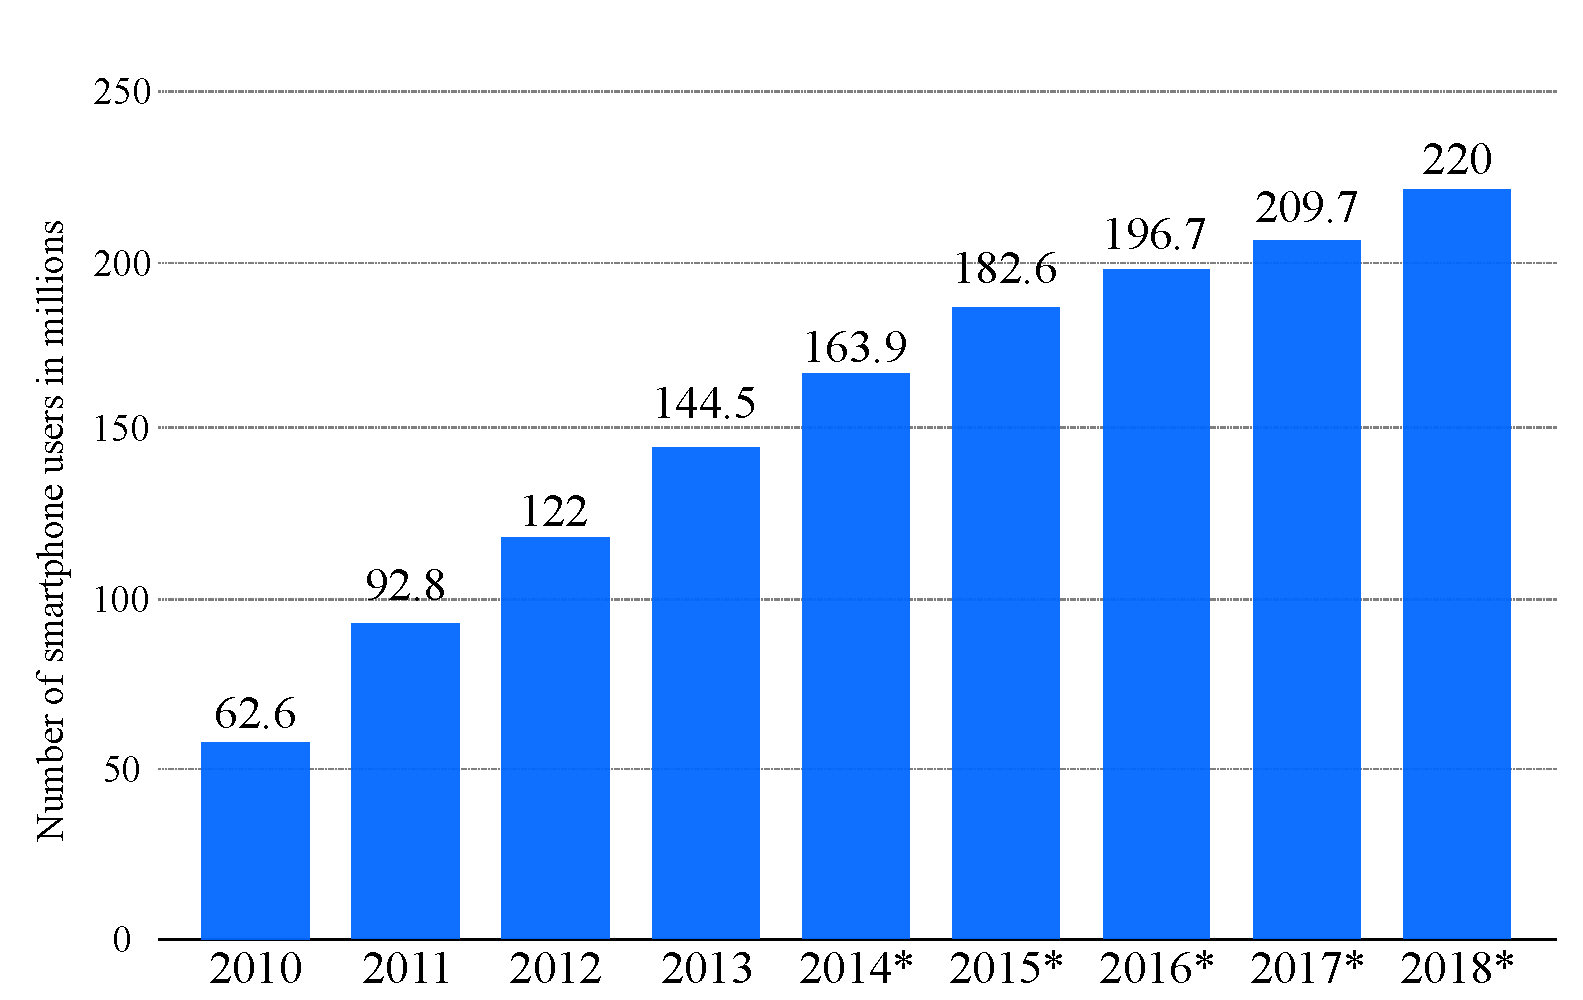
\includegraphics[width=0.85\textwidth]{../figures/PDF/smartphones_boom.pdf}
\caption{Number of smartphone users in the \ac{us} from 2010 to 2018 (in
millions)~\citep{smartphones_boom}. This forecast shows the anticipated number
of smartphone users in the \ac{us} from 2014 to 2018, based on figures from 2010 
to 2013. The source estimates that there will be more than 196 million smartphone
users in the \ac{us} by the year 2016.}
\label{fig:smartphones_boom}
\end{figure}

Another problem deals with the granularity of the model. A generic model might
not be useful for specific scenarios in the same domain, as it would lack specific
parameters. On the other hand, if it is too specific they may not apply well to
other domains. The AdaptUIOnt model tries to address this second aspect by being
abstract regarding the user disabilities. 

Regarding the presented set of rules, it is significant how they represent the
three step adaptation understood by AdaptUI. This is translated into a three
subset of rules which aim to modify and generate new knowledge through a reasoning
process. These subsets, called pre-adaptation, adaptation and post-adaptation rules,
are characterized not only for gathering several rules, but also for being modifiable
by developers through a series of tools provided by the AdaptUI platform. These
tools and their characteristics are detailed in Chapter~\ref{cha:architecture}.

%: ----------------------- introduction file header -----------------------
\begin{savequote}[50mm]
% Let's build a playground on this old battlefield.
There's nothing you can do about it, develop and expose, I feed upon your every 
thought, and so my power grows.
\qauthor{Judas Priest}
\end{savequote}


\chapter{The AdaptUI System Architecture}
\label{cha:architecture}

\ifpdf
    \graphicspath{{4_system_architecture/figures/PNG/}{4_system_architecture/figures/PDF/}{4_system_architecture/figures/}}
\else
    \graphicspath{{4_system_architecture/figures/EPS/}{4_system_architecture/figures/}}
\fi

During this dissertation several problems of adaptive systems have been remarked.
Special attention has been paid to their lack of dynamism, the problems of 
modelling (\textit{what} and \textit{how} to model, the \textit{depth} of the 
model and the \textit{required knowledge} in the domain) and the external 
services and platforms dependency to perform computational complex operations. 
Addressing these issues, this dissertation aims a fully operational mobile 
platform. This chapter describes the three-layered architecture designed for 
the AdaptUI platform. The architecture layers and their modules are depicted in 
Figure~\ref{fig:architecture}.

Each layer of the AdaptUI platform is composed of several modules; each module
aiming to solve a concrete requisite. First, there is the Modelling Layer which
collects information of the user's (non physiological) capabilities and context
and device characteristics to finally build a semantic representation of this
knowledge. Two main modules form the Modelling Layer: the Capabilities Collector
and the Semantic Modeller. On the one hand, the Capabilities Collector's main
goal is to obtain information about each entity. On the other hand, the Semantic
Modeller leads the semantic representation and storage of the information
collected by the Capabilities Collector.

Next, there is the Adaptation Layer, which manages the adaptation process of the
user interface components through the Adaptation Engine. Together with the
Adaptation Engine there is the Adaptation Polisher module. This module aims to
refine the adapted user interface by analysing several usability metrics of the
user interaction.

Finally, there is the Application Layer. This layer provides several tools for
developers to be able to use AdaptUI. Through the provided \ac{api} developers 
are allowed not only to make their applications adaptive, but also to add, edit 
and delete knowledge and rules.

\begin{figure}[H]
\centering
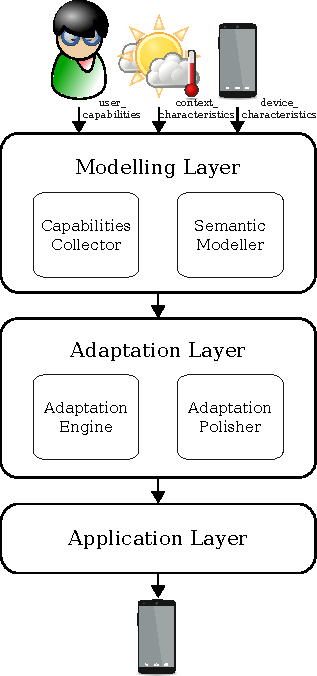
\includegraphics[width=0.30\textwidth]{architecture.pdf}
\caption{AdaptUI's three-layered global architecture.}
\label{fig:architecture}
\end{figure}

In the next sections of this chapter each layer and module is more concretely
explained. First, in Section~\ref{sec:modelling_layer} the Modelling Layer and
its two modules are introduced. The Capabilities Collector is described in
Section~\ref{sec:capabilities_collector}, while the Semantic Modeller is 
detailed in Section~\ref{sec:semantic_modeller}. The Adaptation Layer is 
presented in Section~\ref{sec:adaptation_layer}. This section also details the 
Adaptation Polisher (see Section~\ref{sec:adaptation_polisher}). Next,
Section~\ref{sec:application_layer} presents the characteristics of the 
Application Layer.

In addition, in Section~\ref{sec:architecture_flow}, the relationships among 
the mentioned layers and modules and the flow of the information and knowledge 
within the AdaptUI platform is depicted. Finally, a detailed example is
described in Section~\ref{sec:complete_example} following the information flow
mentioned in Section~\ref{sec:architecture_flow}, highlighting the concrete
tasks performed by each layer and module.


\section{The Modelling Layer}
\label{sec:modelling_layer}

The first layer to be described of the AdaptUI architecture is the Modelling
Layer. This layer aims to generate the different profiles (semantic models) for
the three main entities: the user, the current context and the device. In order
to do this, the Modelling Layer combines the results of two different modules: 
the Capabilities Collector and the Semantic Modeller. The Capabilities Collector
collects information about the three main entities. This module deals with the
current capabilities of the user, the environment current situation, and with
several characteristics of the device, storing the collected information for
further usage. On the other hand, the Semantic Modeller represents the knowledge
gathered and stored by the Capabilities Collector in a semantic model specified
at the AdaptUIOnt ontology (which is fully described in 
Chapter~\ref{cha:ontology_model}). 

The two modules which form the Modelling Layer are described in the following
sections. First, the Capabilities Collector is introduced in
Section~\ref{sec:capabilities_collector}. Next, the Semantic Modeller is
presented in Section~\ref{sec:semantic_modeller}.


\subsection{The Capabilities Collector}
\label{sec:capabilities_collector}

As mentioned in the literature, \citet{fischer_user_2001} defended that the user
evolves through time. More concretely, time and experience are two of the 
reasons for the  evolution of user's characteristics. In AdaptUI users 
evolve, but under different assumptions. Fischer considered long terms 
parameters as the keys for the evolution of the user. On the contrary, AdaptUI 
takes into account temporary and concrete context conditions, limited to a 
specific momentum. Consequently, the user model is built contemplating a dynamic 
user whose capabilities change due to context conditions.

Considering this dynamic user perspective based on several aspects related to
context terms, we discussed how this could be applicable to mobile devices. 
Mobile devices have several characteristics that make them susceptible to change 
(i.e., battery consumption, location awareness, preferences of the screen or 
sound). Thus, in AdaptUI mobile devices are also considered as a dynamic entity.

Finally, regarding the surrounding environment, we consider that it also has the 
propensity to change (i.e., temperature, light or noise). Therefore, within the 
Modelling Layer a concrete module to collect these characteristics has been 
designed: the Capabilities Collector.

The Capabilities Collector is a software module that allows the system gathering 
non physiological capabilities of the user, collect different variables of the 
current environment situation, and identify several device characteristics in 
order to be aware of the whole domain limitations. Figure~\ref{fig:capabilities_collector_flow}
illustrates how the Capabilities Collector uses several activities to collect
the information about the three entities. This information is transferred to the
Semantic Modeller.

\begin{figure}
\centering
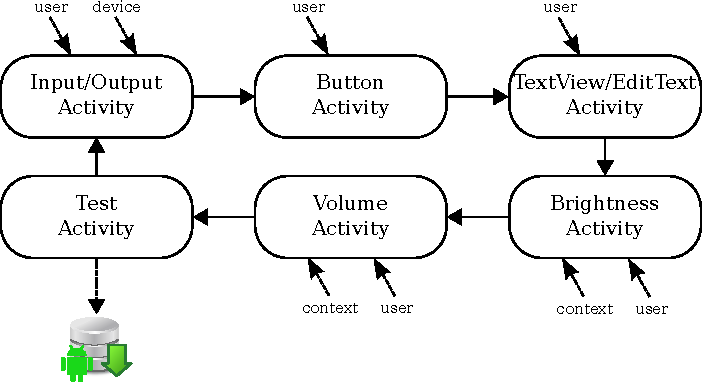
\includegraphics[width=0.65\textwidth]{capabilities_collector_flow.pdf}
\caption{The Capabilities Collector activities and their relationships with the
three main entities in AdaptUI.}
\label{fig:capabilities_collector_flow}
\end{figure}


\subsubsection{Android Activity}
\label{sec:activities}

In Android, activities~\citep{activities}
are application components that provide a screen with which the user can interact.
Each activity is given a window in which to draw its user interface. Android
applications usually consist of multiple activities that bound to each other. 

Android applications have to declare a Main activity. This activity is always
presented to the user when launching the application for the first time. Besides,
activities can start other activities storing their current status (if needed).
An activity lifecycle is illustrated in Figure~\ref{fig:activity_lifecycle}.

\begin{figure}[H]
\centering
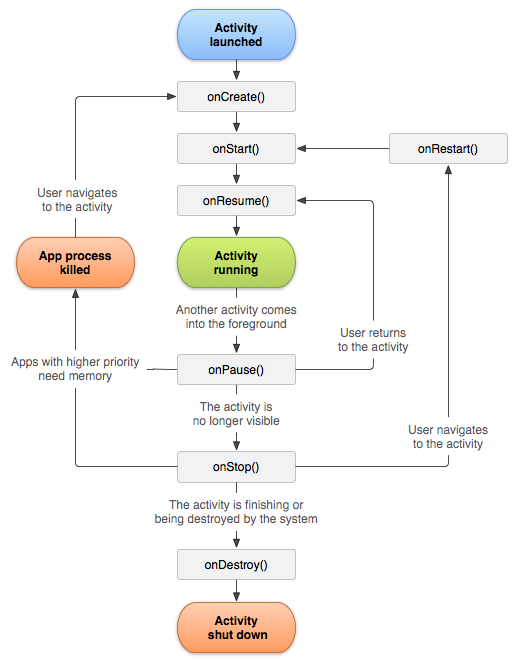
\includegraphics[width=0.55\textwidth]{activity_lifecycle.png}
\caption{The activity lifecycle.}
\label{fig:activity_lifecycle}
\end{figure}

To create an activity the developer has to extend the Activity class. A main
callback method is needed to be implemented: the \textit{onCreate()} method.
The system always calls this method when creating an activity. In it, the
essential components of the activity should be initialized. Besides, and before
any initialization, the \textit{setContentView()} method has to be called. This
method defines the layout for the activity's user interface, which is defined as
an \ac{xml} file in the \textit{layout} folder of the Android project.

Listing~\ref{lst:android_activity} shows an example of an activity initialization.
The layout of the activity is shown in Listing~\ref{lst:activity_layout}. Next,
Figure~\ref{fig:android_activity} illustrates the result of such activity.

\inputminted[linenos=true, fontsize=\footnotesize, frame=lines]{java}{4_system_architecture/android_activity.java}
\captionof{listing}{Example of an activity initialized with a button.\label{lst:android_activity}}

\inputminted[linenos=true, fontsize=\footnotesize, frame=lines]{xml}{4_system_architecture/activity_layout.xml}
\captionof{listing}{An activity layout declaring a button.\label{lst:activity_layout}}

\begin{figure}
\centering
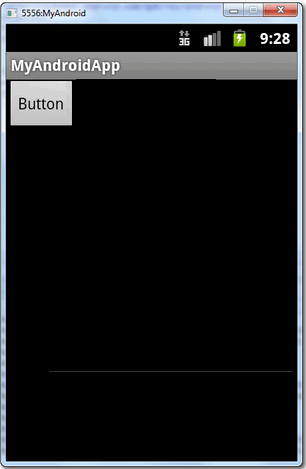
\includegraphics[width=0.35\textwidth]{android_activity.png}
\caption{The resulting activity from the combination of Listing~\ref{lst:android_activity},
Listing~\ref{lst:activity_layout} and Listing~\ref{lst:android_manifest}.}
\label{fig:android_activity}
\end{figure}

It is also important to remember defining the activity in the \textit{AndroidManifest.xml}
file. This file gathers the main specification of the declared activities, filters,
services and allowed permissions, along with the identification of the application.
Listing~\ref{lst:android_manifest} shows an example of a typical manifest file.

\inputminted[linenos=true, fontsize=\footnotesize, frame=lines]{xml}{4_system_architecture/android_manifest.xml}
\captionof{listing}{Application manifest file.\label{lst:android_manifest}}

\subsubsection{Collecting the User's Capabilities}
\label{sec:user_capabilities}

AdaptUI requires the user's capabilities (together with the current context
situation and the characteristics of the mobile device) as an input  for the
adaptation process. As explained in Section~\ref{sec:entities_model}, the user
model of the AdaptUIOnt model does not consider physiological knowledge about
the user. This is due to the lack of physiological and medical background that
users (and developers) of AdaptUI might have, which makes the capabilities
representation inaccurate and impractical. Instead of this, the user model
within the AdaptUIOnt ontology provides a layer of abstraction, focusing on the
user interaction needs. For example, a user who suffers from a hearing disability
in AdaptUI can explicitly configure a minimum sound level, so the system will
not reduce it in any future adaptation. Thus, we avoid modelling specific
physiological problems related to the user's hearing capability. To collect this
kind of information about the user, the Capabilities Collector shows several
screens (known as activities in Android) to the user in which different
interactions are required. 

The first capability that the Capabilities Collector deals with is the input
method or type of interaction. In the AdaptUIOnt ontology this is represented
through the \textit{Interface} class. Through several basic instructions
(presented in text mode and as quick audio question) the user selects his/her
input and output preferences. For example, Figure~\ref{fig:input_activity} shows
the first activity of the Capabilities Collector module. The instructions shown
in this activity can be read by the user and by the application itself (for
example, by using the Android \ac{tts}~\citep{tts} service). Every decision
the user makes is stored in the mobile phone as a profile for a future
\textit{semantization} by the Semantic Modeller.

\begin{figure}
\centering
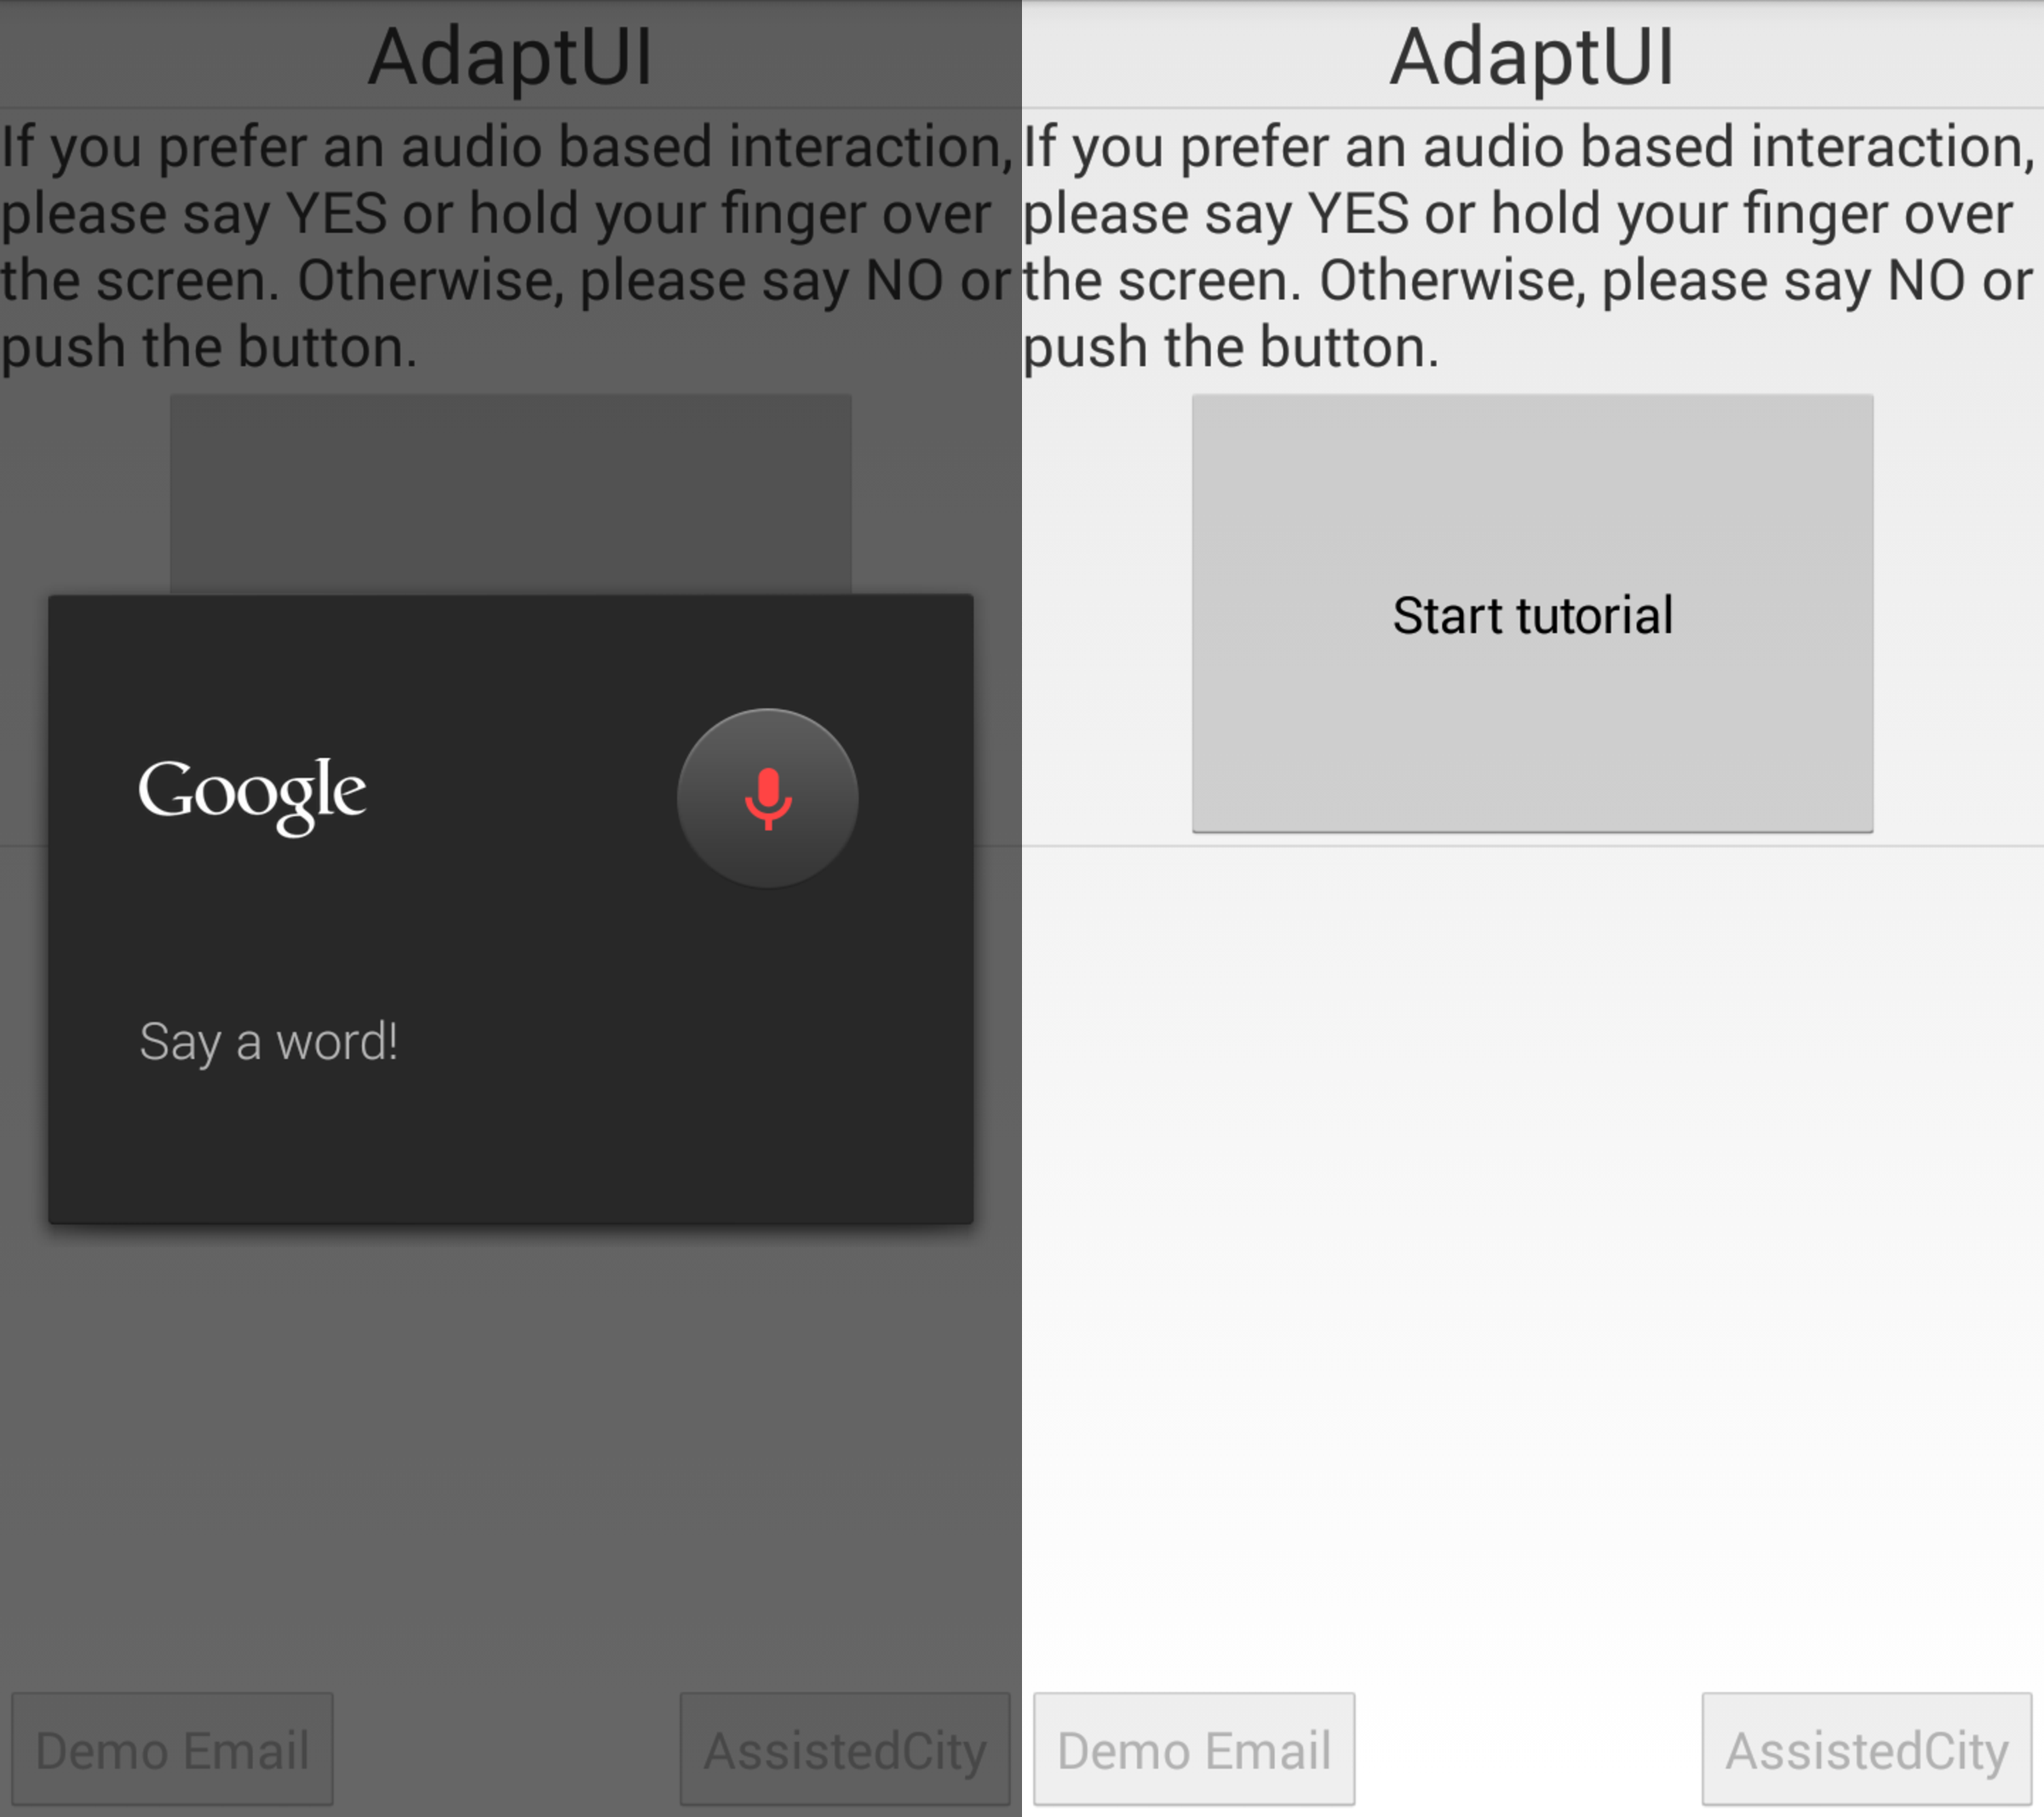
\includegraphics[width=0.50\textwidth]{input_activity.pdf}
\caption{Capabilities Collector's input activity.}
\label{fig:input_activity}
\end{figure}

Once the input interaction type has been determined the output is configured 
accordingly. Next activities show several Android view~\citep{android_view} 
components which are configurable by the user. Views represent the basic 
building block for user interface components in Android. A view occupies a 
particular area on the screen and is responsible for drawing and event 
handling. In this case, a button, a text view and an 
edit text (which is a particular case of a text view) are presented (see 
Figure~\ref{fig:views_activity}). The Capabilities Collector allows the user to 
modify their size, component colour, and also the text size and colour.

\begin{figure}
\centering
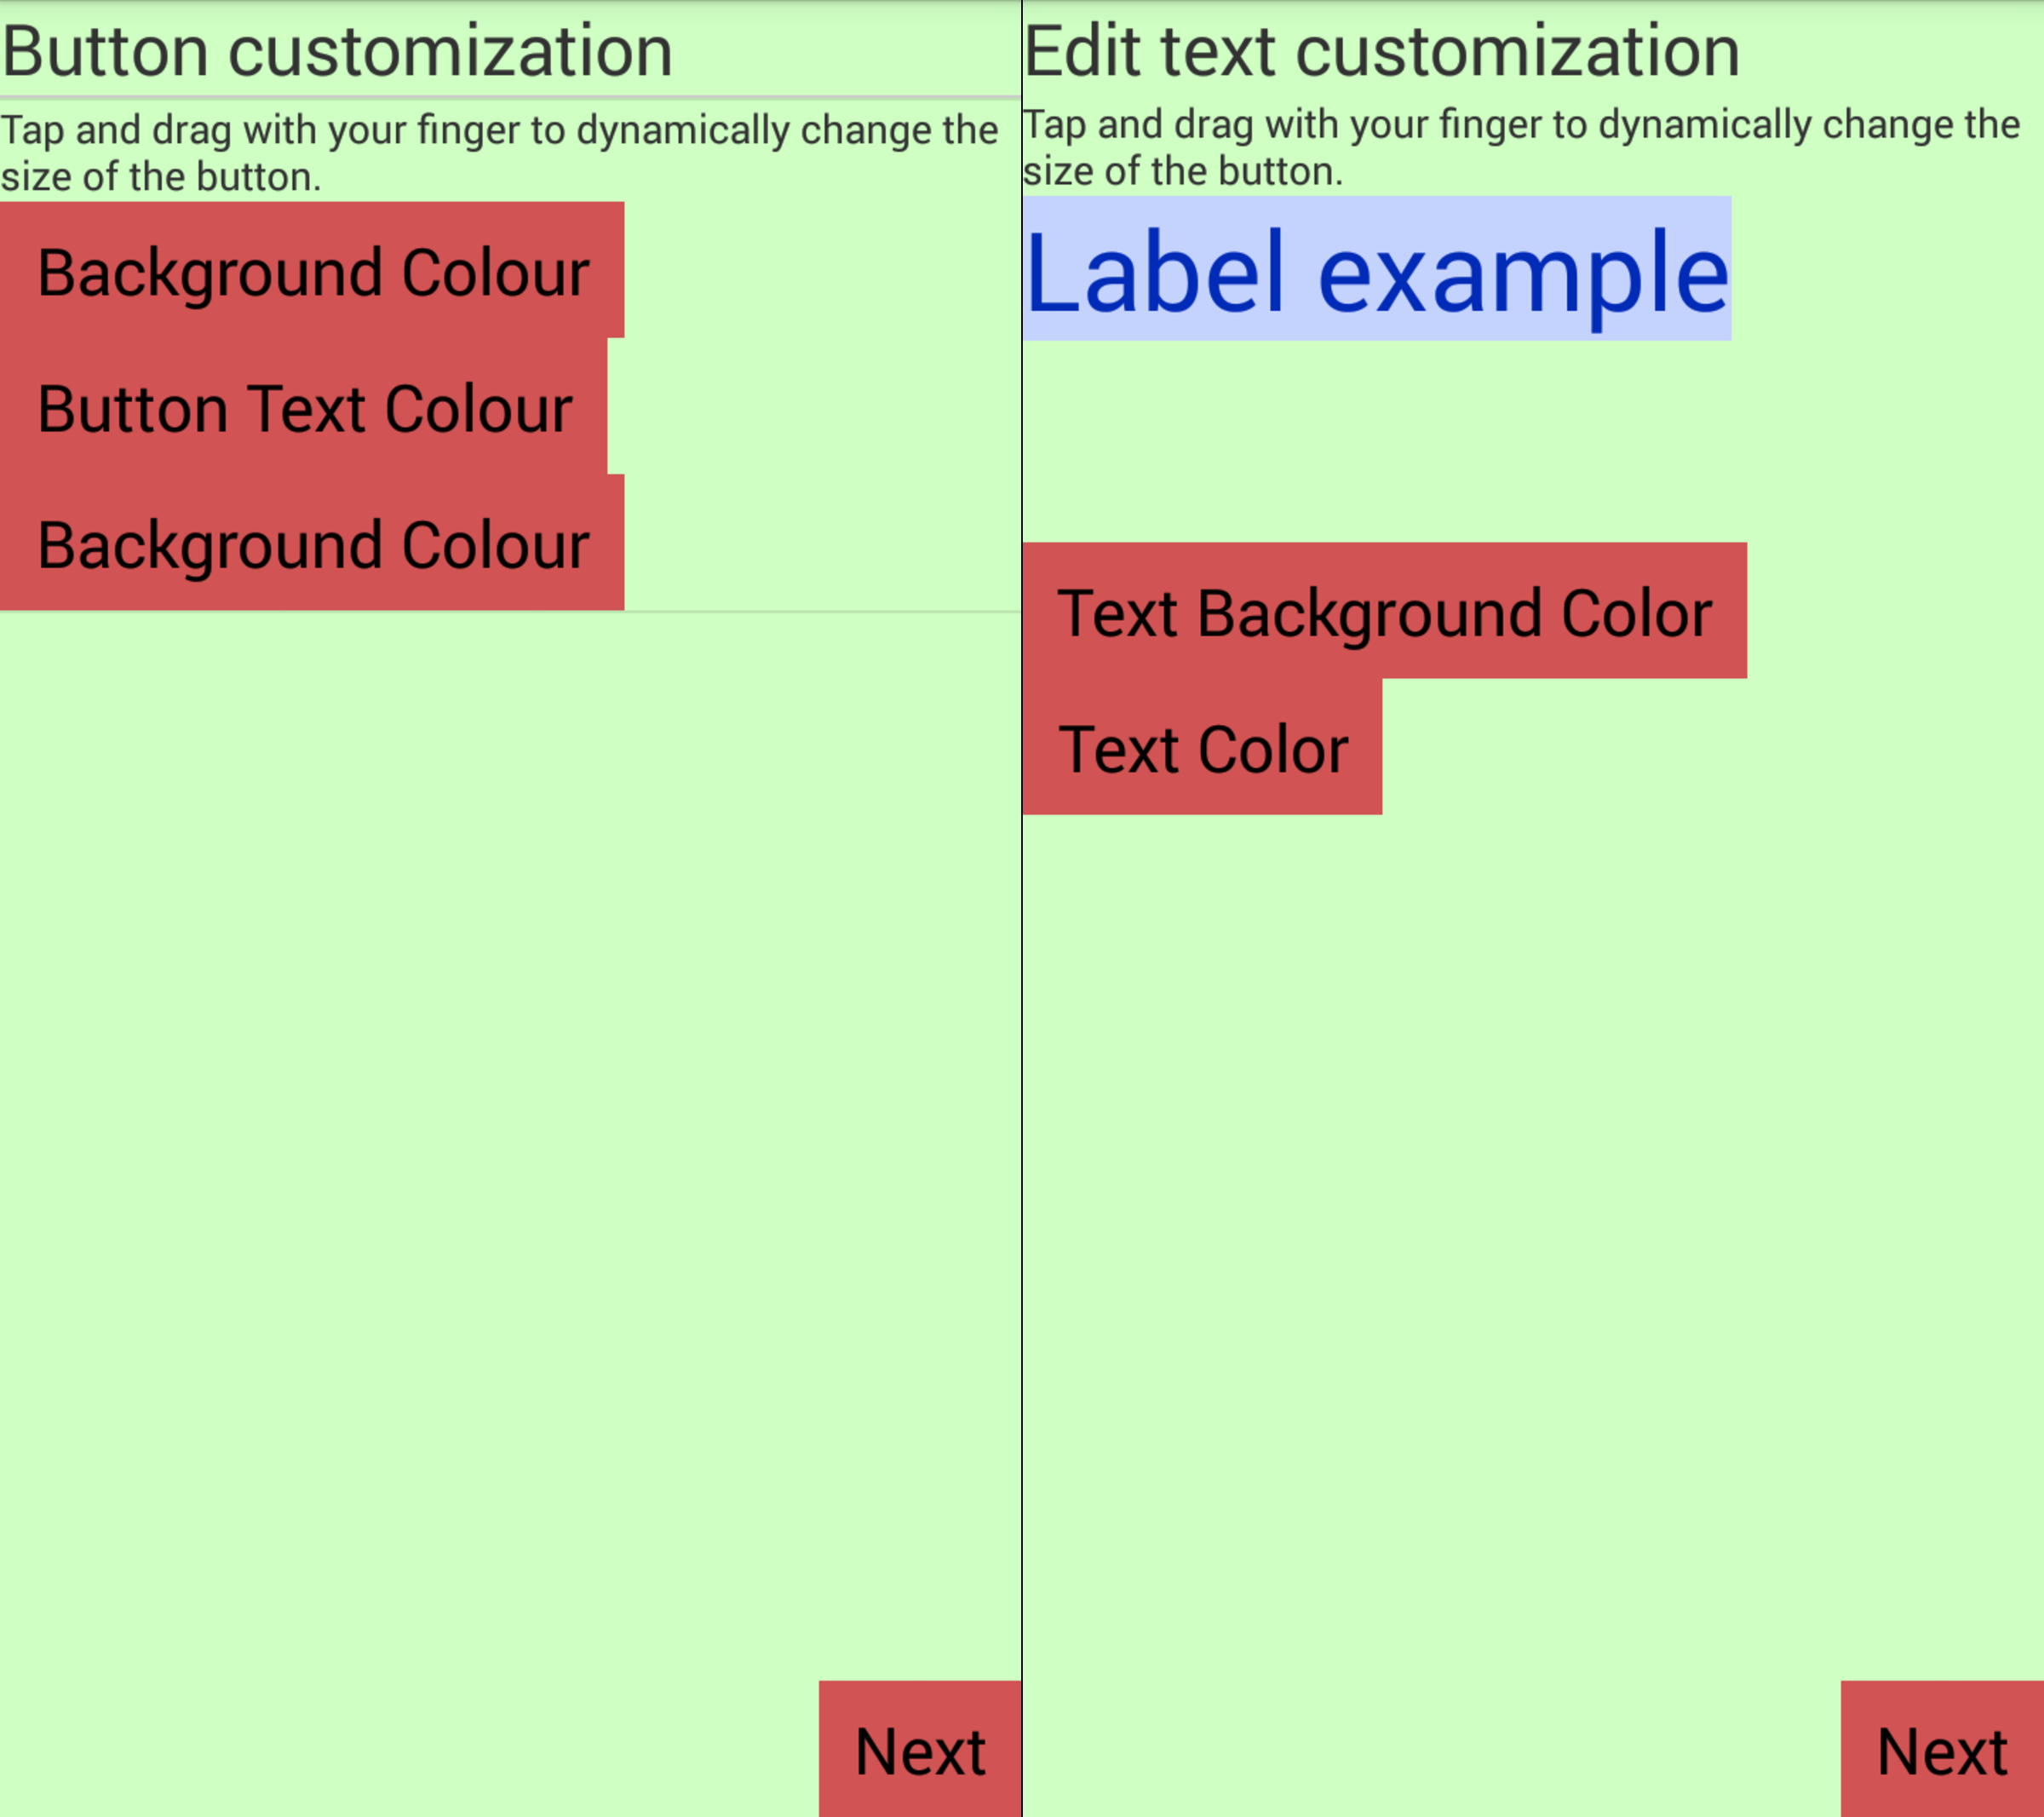
\includegraphics[width=0.50\textwidth]{views_activity.pdf}
\caption{Different Android view components
personalization: on the left, button; on the right, text view and edit text.}
\label{fig:views_activity}
\end{figure}

Finally, the display brightness and the system volume are also allowed to be
customized. The surrounding light and noise are monitored using the available
device sensors, which are listed by the Capabilities Collector when it is first
launched. Thus, AdaptUI is aware of the context conditions and is able to adjust
these parameters to the user's preferences.

 
\subsubsection{The Context Situation}
\label{sec:context_situation}
Current smartphones are equipped with several sensors that allow devices to
collect different environment parameters. Light sensors, microphones, proximity 
sensors for disabling the screen, even Bluetooth and infra-red transceivers are 
just several examples of the hardware available in such devices.

Taking advantage of the current situation, in which smartphones are able to sense
the environment, the Capabilities Collector collects knowledge of the user context.
Light conditions and noise are classified by the Capabilities Collector as follows:

\begin{itemize}
 \item Light conditions are measured in \ac{lx}, which is the \ac{si} unit of 
 luminance~\citep{lux}.
 
 \item The current noise is collected using the mobile available microphones. It
 is measured in \ac{db}, which is a logarithmic unit that expresses the ratio
 between two values of a physical quantity (often power or intensity).
\end{itemize}

Once all this features have been collected, the profile is temporarily stored in 
the device. This storage is carried out using the Android 
SharedPreferences~\citep{shared_preferences}.
This class provides a general persistence framework for developers to save and
retrieve key-value pairs of primitive data types. After this temporary storage
in the device, the Semantic Modeller is the module which deals with the task of
the semantic representation of the model. Listing~\ref{lst:shared_preferences}
shows how developers deal with the SharedPreferences to store and retrieve data
in Android. If complex objects are used, the process is different (see
Listing~\ref{lst:shared_preferences_complex}).

\inputminted[linenos=true, fontsize=\footnotesize, frame=lines]{java}{4_system_architecture/shared_preferences.java}
\captionof{listing}{Using Android SharedPreferences. By default SharedPreferences allows 
to store and retrieve primitive data. Implementing Parcelable allows complex 
objects to be persistent.\label{lst:shared_preferences}}

\inputminted[linenos=true, fontsize=\footnotesize, frame=lines]{java}{4_system_architecture/shared_preferences_complex.java}
\captionof{listing}{Using Android SharedPreferences to store non-primitive
objects.\label{lst:shared_preferences_complex}}

Figure~\ref{fig:context_activity} shows how the brightness and the volume of
the application is configured by a user which is aware of the light and noise
of the environment.

\begin{figure}
\centering
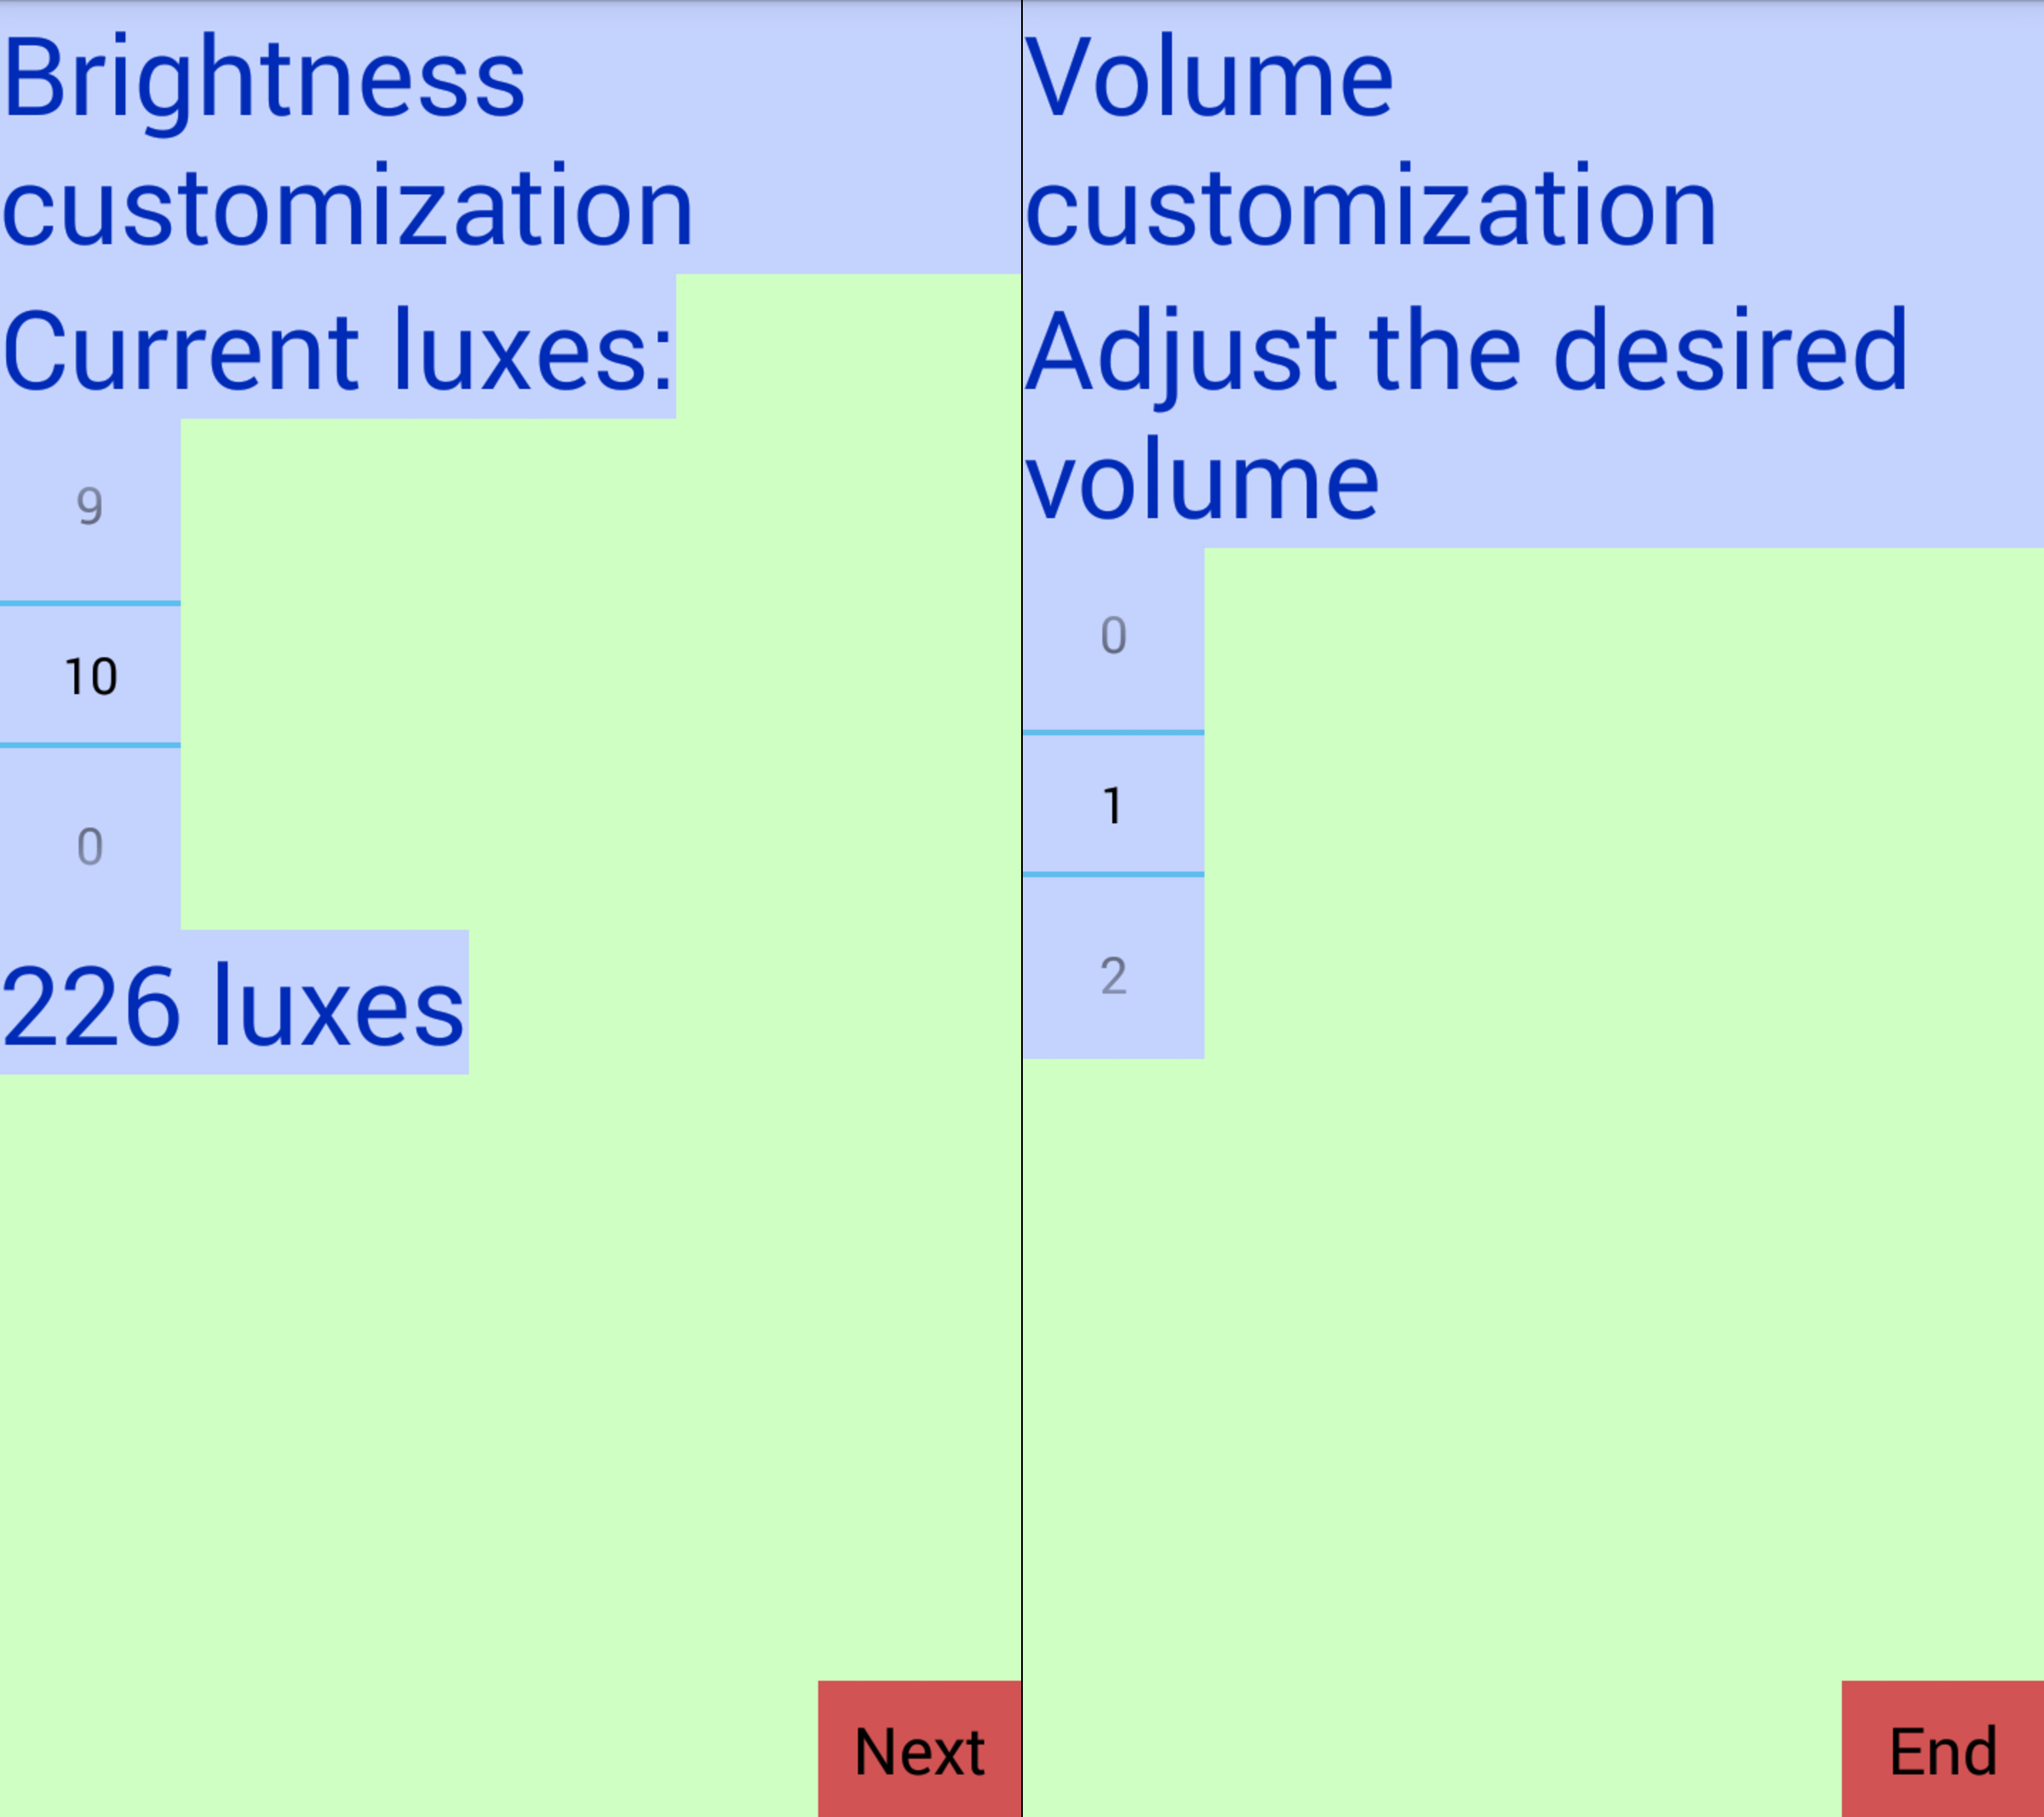
\includegraphics[width=0.50\textwidth]{context_activity.pdf}
\caption{Brightness (left) and Volume (right) adjustment sensing the surrounding
light and noise.}
\label{fig:context_activity}
\end{figure}


\subsubsection{The Device Characteristics}
\label{sec:device_characteristics}

Device characteristics are significant within the AdaptUI platform. These
characteristics limit the possible adaptations of the user interface. For example,
not all the smartphones have the same maximum brightness or sound levels, nor
they have the same connectivity capabilities. Thus, being aware of each device's
capabilities becomes essential in AdaptUI.

The device characteristics are collected by the Capabilities Collector by using
the \textit{Settings.System} class in Android. This class contains global
system-level device preferences. Listing~\ref{lst:device_settings_brightness} 
shows a piece of code which requests the maximum values for the brightness. To 
allow the user to change the brightness of the device's screen a NumberPicker 
element is shown. In its initialization, it is needed to specify the minimum and 
the maximum values of the range. Thus, the user is able to configure the brightness 
to $0$. For the maximum brightness value it is needed to state a default value 
of $1F$.

\inputminted[linenos=true, fontsize=\footnotesize, frame=lines]{java}{4_system_architecture/device_settings_brightness.java}
\captionof{listing}{Android NumberPicker initialization with a minimum value of 0 and a 
maximum value requested to the \textit{Settings.System class}.\label{lst:device_settings_brightness}}


On the contrary, to get values related to audio, the \textit{AudioManager} class
is required. 
% Listing~\ref{lst:device_settings_volume} shows a piece of code with
% which the developer initializes a NumberPicker with the minimum and maximum
% volume levels available in the current device.
% 
% \inputminted[linenos=true, fontsize=\footnotesize, frame=lines]{java}{4_system_architecture/device_settings_volume.java}
% \captionof{listing}{Android NumberPicker initialization with a minimum value of 0 and a 
% maximum value requested to the AudioManager class.\label{lst:device_settings_volume}}


Before asking the user about the way of interaction, the Capabilities Collector
performs an analysis about several device's capabilities. Several hardware
details are collected: processor maximum speed, processor availability, battery
current levels, maximum and current available memory, available input modes, 
and so forth. All the characteristics are shown in Table~\ref{tbl:device_characteristics}. 
These are stored during the process for the Semantic Modeller to store in the 
final model.

\begin{table}[H]
  \caption{Requested device characteristics.}
 \label{tbl:device_characteristics}
\footnotesize
\centering
 \begin{tabular}{l l}
  \hline 
  \textbf{Characteristic}& \textbf{Description}				\\
  \hline
  Brightness		& Describes the current device’s brightness.	\\
  Contrast		& Represents the current device’s contrast.	\\
  Volume		& Describes the current device’s volume.	\\
  Processor		& Models the number of the device’s cores.	\\
  OS version		& Indicates the current	\ac{os} version.	\\
  Acceleration		& Represents the current X, Y, Z acceleration.	\\
  Orientation		& Current orientation of the device.		\\
  Device memory		& Maximum device memory.			\\
  Available memory	& Current available device memory.		\\
  Battery		& Current device battery levels.		\\
  Screen resolution	& Maximum screen resolution.			\\
  Storage		& Maximum available storage.			\\
  Available storage	& Current available storage.			\\
  Processor		& Maximum processor of the device.		\\
  Available processor	& Current processor availability.		\\
  \hline
\end{tabular}
\end{table}


\subsection{The Semantic Modeller}
\label{sec:semantic_modeller}

Once the Capabilities Collector has finished its task, all the collected
knowledge is stored in the mobile. The Semantic Modeller's goal is to build a 
semantic representation of this knowledge through the AdaptUIOnt ontology and
store it in the mobile device. This task requires from a semantic reasoner. 
However, there are no available and remarkable reasoners written in Java and 
compatible with Android. Thus, an Android port of the 
Pellet~\citep{pellet} reasoning engine has been
developed: \textit{Pellet4Android}. As Pellet is available for open source
applications under the terms of the \ac{agpl} version 3 license, the provided
\textit{Pellet4Android} is also available in Github~\citep{pellet4android}
under the same license regulations.

During the following subsections both versions of the Pellet reasoning engine
are presented. First, in Section~\ref{sec:pellet}, the Java based Pellet reasoning
for desktop is introduced. Next, Section~\ref{sec:pellet4android} describes the
process followed to port Pellet to Android.

As the Semantic Modeller finishes storing the corresponding knowledge in the
AdaptUIOnt ontology, several rules are triggered. The main consequence of the
execution of these rules is shown through the \textit{Adaptation} class. This
class is filled with the adaptation values that will be requested by the
Adaptation Layer, which is the next layer of the AdaptUI architecture.


\subsubsection{Pellet}
\label{sec:pellet}

% \begin{description}
%   \item[\Defi{Reasoner by~\citet{owlapi_reasoners}}] \hfill \\
%   \begin{mdframed}[hidealllines=true,backgroundcolor=gray!20]
%   \textit{``A reasoner is a key component for working with \ac{owl} ontologies. 
%   In fact, virtually all querying of an \ac{owl} ontology (and its imports closure) 
%   should be done using a reasoner. This is because knowledge in an ontology 
%   might not be explicit and a reasoner is required to deduce implicit knowledge 
%   so that the correct query results are obtained''}~\citep{owlapi_reasoners}.
%   \end{mdframed}
% \end{description}

Developed by Clarkparsia, Pellet is a free and open source \ac{owl}-\ac{dl}
reasoner written in Java. As a \ac{dl} reasoner, it provides several standard 
inference services:

\begin{itemize}
  \item \textit{\ac{owl}-\ac{dl} consistency checking}: Pellet assures that the 
  knowledge represented in the ontology does not contain contradictory facts. 
  \citet{carroll_owl_2004} define that \textit{``an \ac{owl} consistency checker 
  takes a document as input, and returns one word being Consistent, Inconsistent, 
  or Unknown.''} In \ac{dl} terminology  this is the operation to check the 
  consistency of an ABox with respect to a TBox (see the description of this 
  \ac{dl} terminology in Table~\ref{tbl:dl_terms}).
  
  \item \textit{Concept satisfiability}: Determines whether it is possible for 
  a class to have any instances. This avoids cases in which unsatisfiable classes 
  might define instances, which will cause the ontology to be inconsistent.
  
  \item \textit{Classification}: Pellet is able to create the complete class 
  hierarchy from the computation of the subclasses relations between every 
  named class. This allows performing future queries (i.e., getting all the 
  direct subclasses of a class).
  
  \item \textit{Realization}: It is able to find the most specific classes that 
  an individual belongs to. Realization directly depends on classification, and 
  it cannot be done without it.
\end{itemize}


\begin{table}[H]
  \caption{Several \ac{dl} terminology.}
 \label{tbl:dl_terms}
\footnotesize
\centering
 \begin{tabular}{l l}
  \hline 
  \textbf{Component} 		& \textbf{Description}				\\
  \hline
  ABox (Assertional Box)	& Contains assertions about individuals	\\
				& (i.e., \ac{owl} facts such  as type, property	\\
				& -value, equality or inequality assertions).	\\
  TBox (Terminological Box)	& Contains axioms about classes, i.e., \ac{owl}	\\
				& axioms such as subclass, equivalent class 	\\
				& or disjointness axioms.			\\
  \acl{kb}			& A combination of ABox and TBox (i.e.,		\\
				& a complete ontology).				\\
  \hline
  
\end{tabular}
\end{table}

The reasoning capabilities of Pellet are accessible through different interfaces.
For example, Pellet is directly integrated with the Protégé ontology 
editor~\citep{protege}. Thus, reasoning capabilities
are allowed through the user interface of this editor. For developers, there are
several tools provided as \acsp{api} which allow the utilisation of Pellet. The
most significant ones are Apache Jena~\citep{jena}
and Manchester \ac{owl}-\ac{api}~\citep{owlapi}:

\begin{itemize}
  \item Jena: Apache Jena (or Jena) is a free and open source framework written
  in Java which allows building semantic web and Linked Data applications. The
  framework is composed of different \acp{api} interacting together to process 
  \ac{rdf} data.
  
  \item \ac{owl}-\ac{api}: Available under \ac{lgpl} or Apache Licenses, the 
  \ac{owl}-\ac{api} is an open source high level \ac{api} maintained by the 
  University of Manchester for working with \ac{owl} ontologies. Closely aligned 
  with the \ac{owl} 2 structural specification, the \ac{owl}-\ac{api} supports 
  parsing and rendering in the syntaxes defined in the \ac{w3c} specification 
  (i.e., Functional Syntax, \ac{rdf}/\ac{xml}, \ac{owl}/\ac{xml} and the 
  Manchester \ac{owl} Syntax), the manipulation of ontological structures, and 
  the use of reasoning engines (i.e., Chainsaw, FaCT++, JFact, HermiT, Pellet 
  and RacerPro).  
\end{itemize}

% The core of the system is the tableaux reasoner. This reasoner checks the
% consistency of a knowledge base and allows Pellet to support \ac{swrl}~\citep{swrl}
% rules language.


\subsubsection{Reasoning with Pellet in Android: Pellet4Android}
\label{sec:pellet4android}

The AdaptUI platform was conceived to support reasoning and semantic knowledge
representation due to the benefits that ontologies bring. Nevertheless, after
analysing the possibilities and solutions provided by the community (i.e., mobile
reasoning platforms) we found that, although nowadays mobile capabilities allow
heavier processing, there are no remarkable efforts in the area.

\citet{yus_android_2013} noticed this issue and made great efforts porting
several Java based reasoners to Android. Although the authors do not provide the
developed ports to the community, they provide several instructions to make these
reasoners available for Android devices. Thus, following these instructions a port
of Pellet has been developed for AdaptUI: \textit{Pellet4Android}.

As Pellet, \textit{Pellet4Android} also supports full \ac{owl} 2 and \ac{dl} 
rules. To make Pellet run in Android the following steps were needed:

\begin{itemize}
  \item Pellet uses Jena, which is a free and open source framework written in
  Java which allows building semantic web and Linked Data applications. However,
  Jena is not directly importable to Android. Thus, it is necessary to replace it
  with Androjena~\citep{androjena}. Androjena
  is a porting of Hewlett-Packard's Jena semantic web framework to Android. 
  
  \item Pellet also imports the \ac{jaxb} library~\citep{jaxb} for \ac{xml} 
  parsing. \ac{jaxb} is able to translate \ac{xml} Schemas building a set of 
  classes that correspond to that schema. It originally comes with the Java 1.6 
  release, but its easily importable to previous Java version integrating the 
  \ac{jaxb} jar files. The problem is that \ac{jaxb} uses classes that are not 
  compatible with Android. Thus, this package has been removed. 
  
  \item As the official Oracle documentation states, the \textit{javax.xml.bind}
  package \textit{``provides a runtime binding framework for client applications
  including unmarshalling, marshalling, and validation capabilities''}~\citep{javax_xml_bind}.
  Nevertheless, this package is also incompatible with Android, and we should
  remove it from the package list and the build path.
  
  \item Also related with the way Java manages \ac{xml} files, the 
  \textit{org.apache.xerces}~\citep{xerces} package
  is used for the creation and maintenance of \ac{xml} parsers and related
  software components. Several classes under this package are not importable by
  Android, so the package has to be removed.
  
  \item Finally, under the \textit{com.clarkparsia.pellet} package there are several
  classes that are not directly importable by Android. Thus, without removing them,
  we have to search the specific troublesome lines of code (usually related with
  concrete data types and exceptions) and comment them. 
\end{itemize}

Figure~\ref{fig:pellet4android} shows the package structure of the
\textit{Pellet4Android} port and the imported libraries in the Android project.
% 
% \InsertFig{pellet4android}{fig:pellet4android}{Package structure (left) and 
% needed libraries (right) for Pellet4Android}{}{0.85}{}

\begin{figure}[H]
\centering
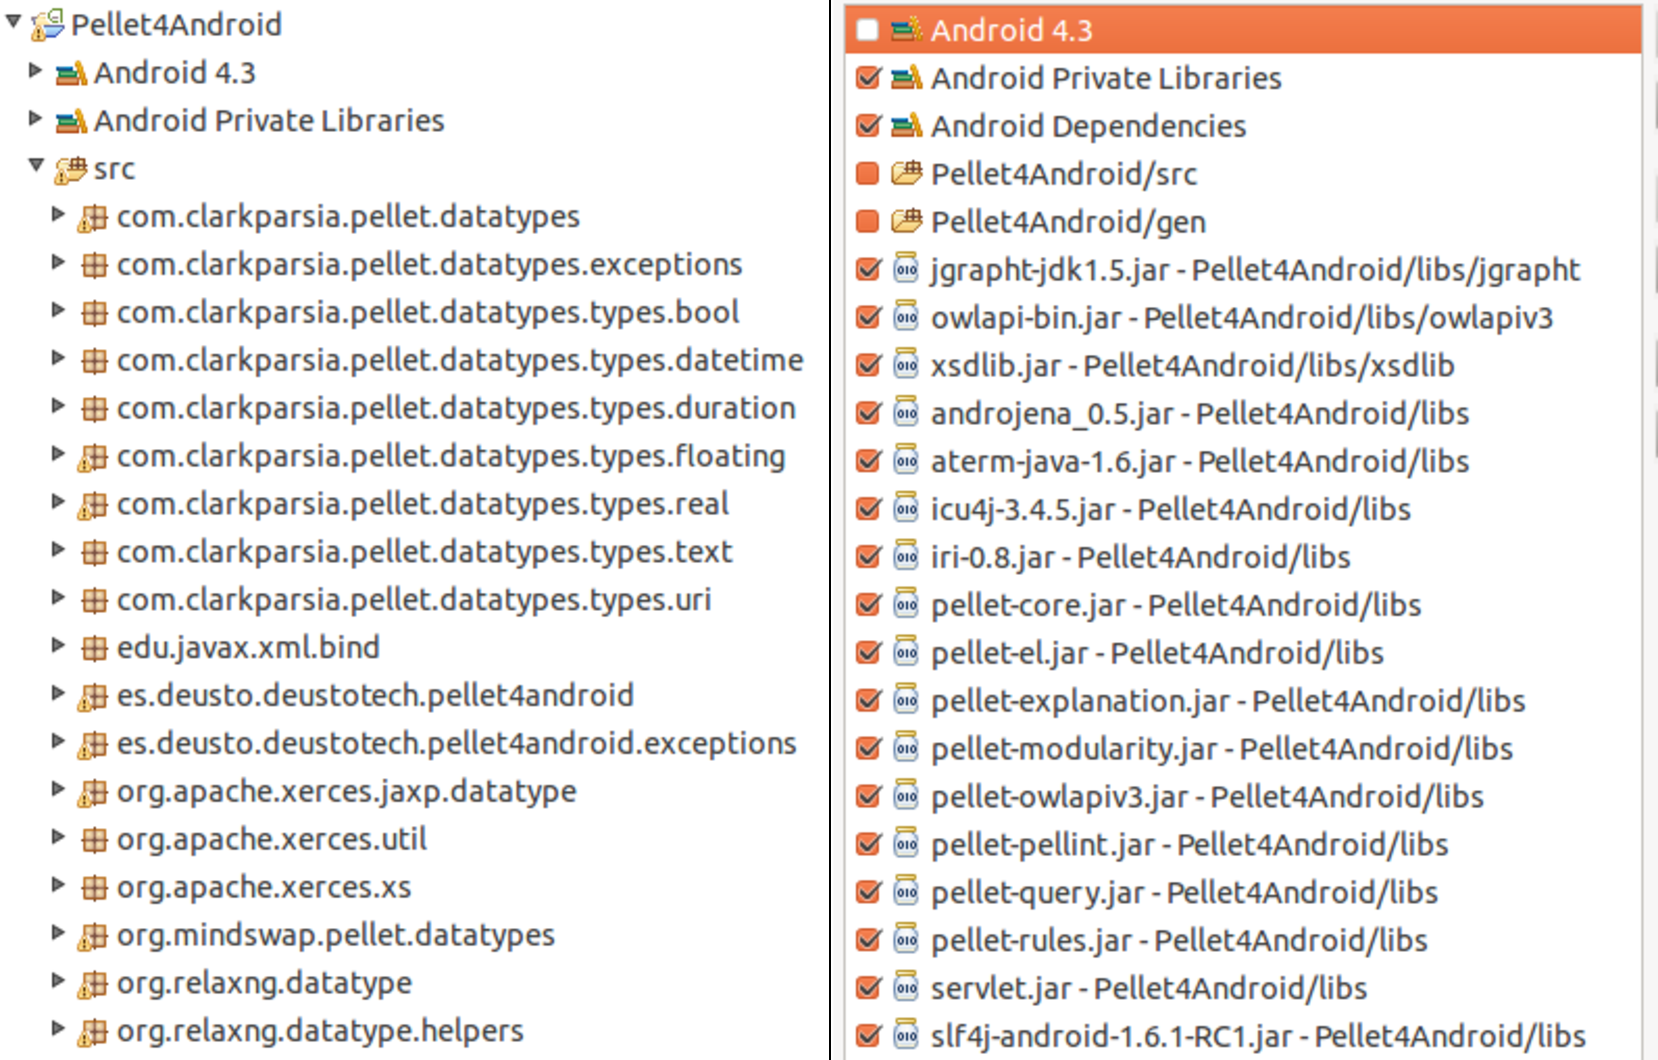
\includegraphics[width=0.85\textwidth]{pellet4android.pdf}
\caption{Package structure (left) and needed libraries (right) for Pellet4Android.}
\label{fig:pellet4android}
\end{figure}


As~\citet{yus_android_2013} remarked, it is important to provide a larger heap
size. To do this, the \textit{android:largeHeap} tag of the AndroidManifest.xml 
file of the project has to be changed to \textit{true}.

A first evaluation of the port was carried out by~\citet{yus_android_2013}.
Nevertheless,~\citet{bobed_android_2014} performed a second evaluation of the
Pellet version for Android obtaining promising results in terms of efficiency
and time responsiveness. Although in this dissertation a similar approach to port 
Pellet has been followed, it is impossible to be a 100\% sure if the results are 
the same (as the version by~\citet{yus_android_2013} was not available for testing). 
Thus, in Chapter~\ref{cha:evaluation} an evaluation of \textit{Pellet4Android} is 
included.


\section{The Adaptation Layer}
\label{sec:adaptation_layer}

The second layer of the AdaptUI architecture is the Adaptation Layer. After the
processes performed by the Modelling Layer, the Adaptation Layer aims to lead the
dynamic adaptation of the elements presented in the user interface. It is formed
by two different modules: The Adaptation Engine, whose purpose is to adapt the
currently interface shown by the device, and the Adaptation Polisher, which aims
the refinement of the user interface basing its task in several usability metrics.


\subsection{The Adaptation Engine}
\label{sec:adaptation_engine}

After the storage of the domain knowledge in the AdaptUIOnt ontology by the
Semantic Modeller, several rules are triggered. These rules are grouped in three
different subsets: the pre-adaptation rules, the adaptation rules and the post-adaptation
rules. More concretely, the adaptation rules subset is the one which modifies
the knowledge represented by the \textit{Adaptation} class in the AdaptUIOnt
ontology.

Once these rules have been executed the Adaptation Engine requests these results
to the \textit{Adaptation} class. Then, it launches several methods to dynamically
change the aspect of the current user interface. These methods basically redraw
and refresh the different components shown in the current activity, sharing
their new characteristics to the rest of activities. 

Listing~\ref{lst:redraw} shows an example of how several views are redrawn.
First, the elements that are part of the activity (i.e., buttons and textviews)
are initialized (similarly to other applications). Next, several methods regarding
the adaptation are called. The \textit{redrawViews()} method takes into account
the user's configured profile through the Capabilities Collector and adapts the
components of the activity accordingly. Every activity overwrites this method
(and others), as they extend from a parent abstract class called
\textit{AbstractActivity}. This class mainly manages the services initialization
(e.g., TextToSpeech) and the ontology. 
% Listing~\ref{lst:abstract_activity} shows
% part of the AdaptUI source code where the ontology is initialized.


\inputminted[linenos=true, fontsize=\footnotesize, frame=lines]{java}{4_system_architecture/redraw.java}
\captionof{listing}{Example of the creation and adaptation of an activity. In this case 
the example is centred in the adaptation of a button.\label{lst:redraw}}

% \inputminted[linenos=true, fontsize=\footnotesize, frame=lines]{java}{4_system_architecture/abstract_activity.java}
% \captionof{listing}{The AbstractActivity class ontology related methods.\label{lst:abstract_activity}}

Listing~\ref{lst:store_in_ontology} shows a piece of source code where the developer
uses the \ac{owl}-\ac{api} to store the user profile in the AdaptUIOnt model. 
% The methods called in this example are part of the Turambar framework~\citep{david_ausin_probabilistic_2014}. 
% This framework provides a high-level \ac{api} for managing the \ac{owl}-\ac{api}.

\inputminted[linenos=true, fontsize=\footnotesize, frame=lines]{java}{4_system_architecture/store_in_ontology.java}
\captionof{listing}{Inserting values in the corresponding classes of the AdaptUIOnt 
ontology.\label{lst:store_in_ontology}}


Finally, Figure~\ref{fig:adaptation_differences} shows two activities with the
same user interface. The difference is that the activity on the left is showing
the default user interface defined in the activity's layout. On the contrary,
the activity on the right shows adapted components.

\begin{figure}[H]
\centering
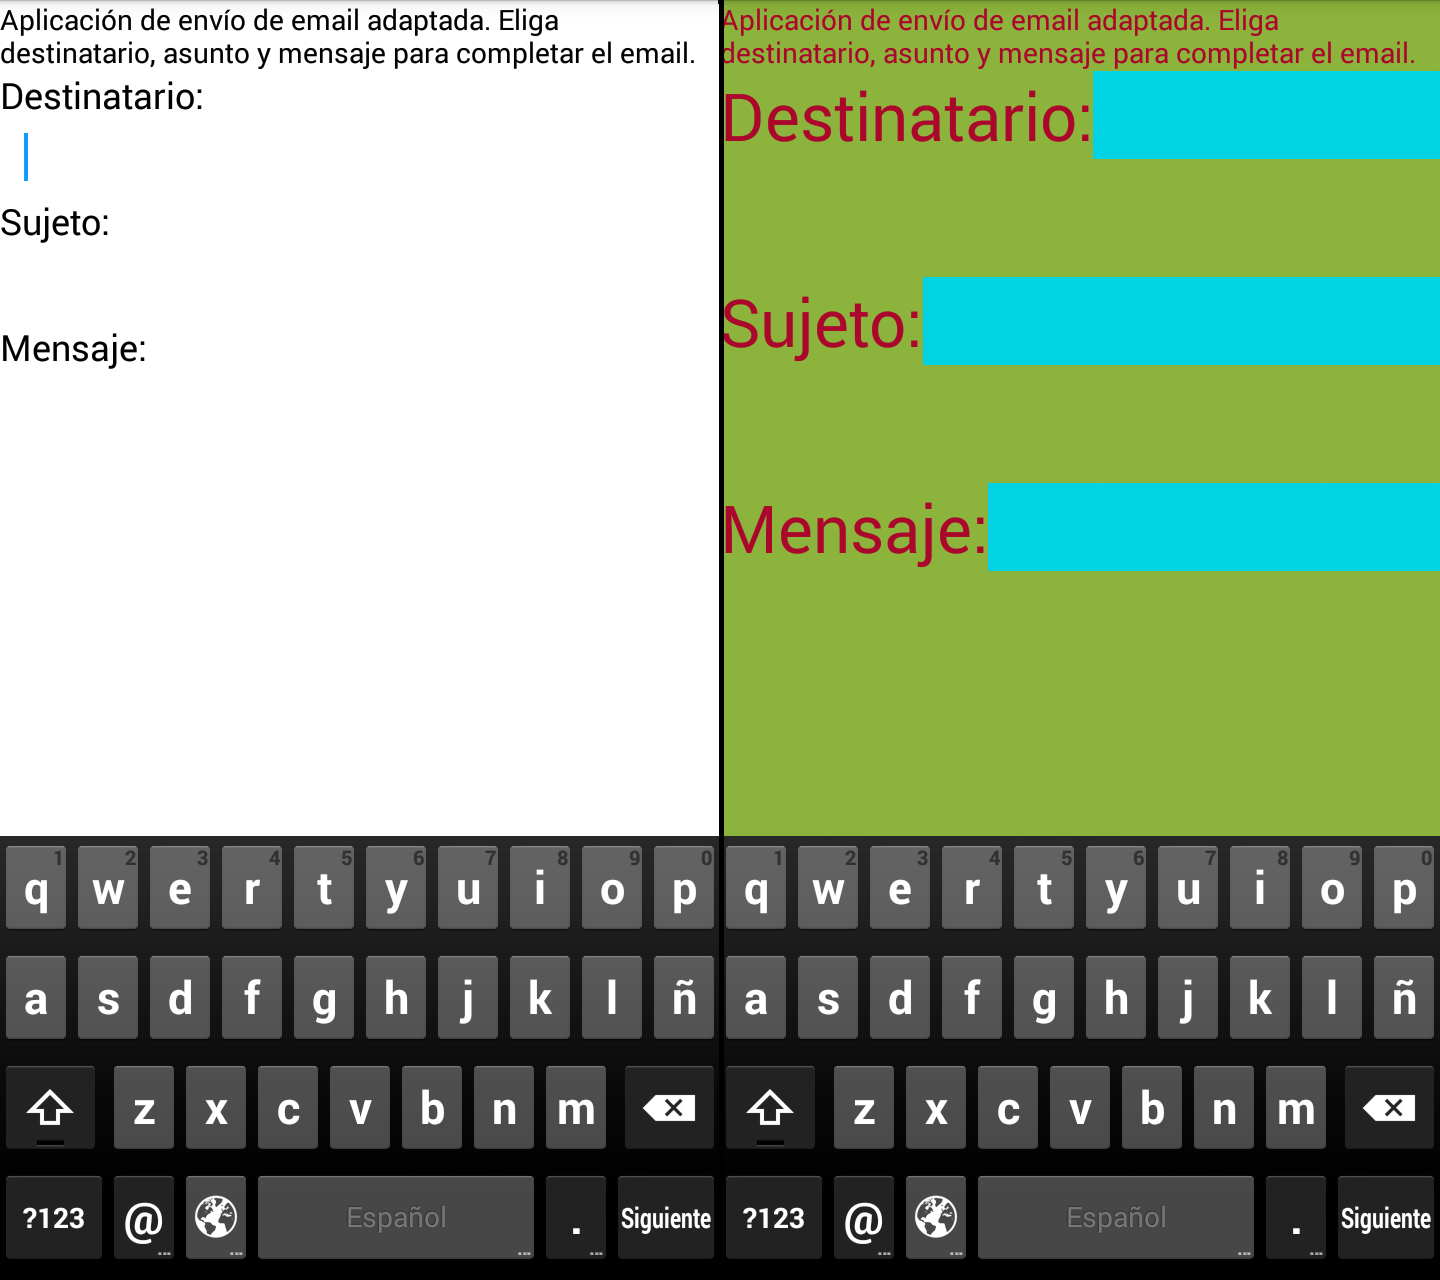
\includegraphics[width=0.65\textwidth]{adaptation_differences.png}
\caption{User interface adaptation performed by the Adaptation Engine. On the
left, a default activity with no adaptation. On the right, the same activity
after the adaptation process. As is shown, the colours sets and sizes of each
component of the adapted user interface are different from the non adapted one.}
\label{fig:adaptation_differences}
\end{figure}


\subsection{The Adaptation Polisher}
\label{sec:adaptation_polisher}

Although the adaptations for the user follow the instructions detailed by him/her,
there is still the possibility that the Adaptation Engine's results lead to a
unsuccessful interaction/adaptation. One of the main reasons for this is that
the classification of the model, considering the context aspects, is just an
approximation of the reality. For example, considering that between 1,000 \ac{lx} and
25,000 \ac{lx} the reasoner determines that the ontology value for the luminance
is \textit{daylight}, the difference might be significant in real scenarios
(see Table~\ref{tbl:luminance}). In other words, the user might easily interact
with a 1,000 \ac{lx} context light but tediously in a 24,999 \ac{lx} light environment. In
order to tackle this problem, there are two possible solutions: to consider
an extensive set of classification rules including more possible situations (e.g.,
dividing the luminance table into more categories), or to design a specific
module which evaluates the user interaction results: the Adaptation Polisher.

The first case is difficult to implement. Nevertheless, AdaptUI provides an \ac{api}
which aims to help in this issue allowing developers to create and modify the
ontology knowledge. This means that it is possible to try to model every tiny
context variation to capture different context characteristics and adapt the user
interface accordingly. However, this is not practical, and AdaptUI covers the
second case with the Adaptation Polisher. Therefore developers do not have to
model these small variations in the environment.

The Adaptation Polisher is a software module, part of the Adaptation Layer, which
monitors the effectiveness and responsiveness of the adapted interfaces. Collecting
different usability and productivity metrics of the interaction carried out by the
user, this module is able to make small but specific adaptations to improve
the ongoing interaction. This module has been designed considering the relative
user efficiency productivity metrics. These metrics compare the efficiency of the
user compared to an expert. But it has no sense to compare the user with others
in AdaptUI. The system cannot generalize and apply adaptations based on other
users' preferences. To solve this, in AdaptUI we propose to maintain a base
adaptation, which thanks to the Adaptation Polisher and its interaction results
will be improved. Consequently, an interaction model is built for each adaptation.
Therefore, we can determine the efficiency of the user when he/she is manipulating
an adaptation made by the system by comparing the last adaptation to the previous
one.

% AdaptUI keeps an interaction model of the user (as an expert) stored in the
% ontology. Once an adaptation is made, the Adaptation Polisher monitors the user
% interaction and then checks the stored model with the new generated one. Next,
% the post-adaptation rules are triggered.


\subsubsection{The Usability Metrics}
\label{sec:usability_metrics}
For this module, several usability metrics have been studied and implemented.
These metrics are classified into two different groups: \textit{effectiveness}
metrics and \textit{productivity} metrics. Table~\ref{tbl:effectiveness_metrics}
and Table~\ref{tbl:productivity_metrics} detail the usability metrics implemented
in AdaptUI. The following information is given for each metric in the cited
tables:

\begin{enumerate}[label=\alph*)]
  \item Purpose of the metric: Expresses the main goal of the current metric.
  \item Measurement, formula and data element computations: Provide the formulas
  to compute the current metric and the meaning of the used data elements.
  \item Interpretation of the measured value: Details the range and preferred values.
  \item Metric scale type: Provides the type of scale used by the current metrics.
  The possible scale types are: Nominal, Ordinal, Interval, Ratio and Absolute
  scale.
  \item Measure type: Provides the type of the measure. The possible measure
  types are: Size, Time and Count.
\end{enumerate}

In the original \ac{iso} document~\citep{ISOIEC9126} there are 4 extra columns that
have not been included in Table~\ref{tbl:effectiveness_metrics} and
Table~\ref{tbl:productivity_metrics}. This is because the values for each metric
under these columns are the same:

\begin{enumerate}[label=\alph*)]
  \item Method of application: Provides an outline of the application. 
  
  \item Input to measurement: Details the source of data used in the measurement.
  In this case there are two inputs that each metric shares: Operation (test) 
  report and User monitoring record.
  
  \item Reference: Identifies software life cycle processes where the metric is
  applicable. There are three processes that each metric shares: 6.5 Validation,
  5.3 Qualification testing and 5.4 Operation.
  
  \item Target audience: Identifies the user(s) of the measurement results. Again,
  the metrics share User and Human interface designer as their audiences.
\end{enumerate}


\myparagraph{Effectiveness Metrics}
\label{sec:effectiveness_metrics}
Effectiveness metrics, as detailed in the \ac{iso}/\ac{iec} 9126-4~\citep{ISOIEC9126},
evaluate whether the current task achieves a specific goal considering the accuracy
and completeness of the corresponding task. These metrics are shown in
Table~\ref{tbl:effectiveness_metrics}.


% \begin{landscape}
\begin{table}
  \caption{The effectiveness metrics used in the Adaptation Polisher, as it appears in~\citep{ISOIEC9126}.}
 \label{tbl:effectiveness_metrics}
\footnotesize
\centering
 \begin{tabular}{l l l l l l}
  \hline 
\textbf{Metric}	& \textbf{Purpose of }	& \textbf{Measurement,}		& \textbf{Interpretation }	& \textbf{Metric}	& \textbf{Measure} 	\\
\textbf{name}   & \textbf{the metrics}	& \textbf{formula and data}	& \textbf{of measured }		& \textbf{scale}   	& \textbf{type}		\\
		& 			& \textbf{element compu-}	& \textbf{value}		& \textbf{type}					\\
		& 			& \textbf{tations}												\\
\hline
Task  		& To measure the 	& $M1=|1-\Sigma A_{i}|$		&  $0\leq M1 \leq 1$		& \textemdash 		& $A=$ proportion 	\\
effectiveness	& proportion of the  	& 				&				& 			& 			\\
		& goals of the task	& $A_{i}=$ proportional  	& The closer to			& 			& 			\\
		& achieved 		& value of each 		& 1.0 the better.		& 			& 			\\
		& correctly.		& missing or incorrect 		& 				& 			& 			\\
		& 			& component in the 	\\
		& 			& task output		\\
\hline	  
Task  		& To measure the 	& $X=A/B$			& $0\leq X \leq 1$    		& Ratio 		& $A=$ Count 		\\
completion 	& proportion of  	& 				& 				& 			& $B=$ Count		\\
		& the task that 	& $A=$ number of 		& The closer to			& 			& $X=$ Count/Count	\\
		& is completed.		& tasks completed		& 1.0 the better.		& 			& 			\\  
		& 			& $B=$ total number of		& 				& 			& 			\\
		& 			& tasks attempted	\\
\hline
Error  		& To measure the 	& $X=A/T$			& $0\leq X$  	  		& Absolute 		& $A=$ Count 		\\
frequency 	& frequency of 		& 				& 				& 			&~			\\
		& errors.		& $A=$ number of 		& The closer to			& 			&~			\\
		& 			& errors made by the 		& 0 the better.			& 			&~			\\  
		&			& user			\\
		& 			& $T=$ time or number 		& 				& 			& 			\\
		& 			& of tasks 		\\
\hline

\end{tabular}
\end{table}

% \end{landscape}


\myparagraph{Productivity Metrics}
\label{sec:productivity_metrics}
Productivity metrics evaluate the resources consumed by the users in relation
to the effectiveness achieved in the current task~\citep{ISOIEC9126}. These 
metrics are shown in Table~\ref{tbl:productivity_metrics}.


% \begin{landscape}
\begin{table}
  \caption{The productivity metrics used in the Adaptation Polisher, as it appears in~\citep{ISOIEC9126}.}
 \label{tbl:productivity_metrics}
\footnotesize
\centering
  \begin{tabular}{l l l l l l}
  \hline 
\textbf{Metric}	& \textbf{Purpose of }	& \textbf{Measurement,}		& \textbf{Interpretation }	& \textbf{Metric}	& \textbf{Measure} 	\\
\textbf{name}   & \textbf{the metrics}	& \textbf{formula and data}	& \textbf{of measured }		& \textbf{scale}   	& \textbf{type}		\\
		& 			& \textbf{element compu-}	& \textbf{value}		& \textbf{type}					\\
		& 			& \textbf{tations}												\\
\hline
Task  		& To measure the 	& $X=Ta$			& $0\leq X$			& Interval 		& $T=$ Time	 	\\
time		& required time to	& 				&				& 			& 			\\
		& complete the task.	& $Ta=$ Task time		& The closer to			& 			& 			\\
		& 		 	& 				& 1.0 the better.		& 			& 			\\
\hline	  
Task  		& To measure how 	& $X=M1/T$			& $0\leq X \leq 1$    		& \textemdash 		& $T=$ Time		\\
efficiency 	& efficient the 	& 				& 				& 			& $X=$ proportion/	\\
		& users are.		& $M1=$ task 			& The larger the		& 			& time			\\
		&			& effectiveness			& better.			& 			& 			\\
		& 			& $T=$ task time		& 				& 			& 			\\  
\hline
Economic  	& To measure the	& $X=M1/C$			& $0\leq X$  	  		& \textemdash 		& $C=$ Value 		\\
productivity 	& cost-effectiveness	& 				& 				& 			&~			\\
		& of the user.		& $M1=$ task 			& The larger the		& 			&~			\\
		& 			& effectiveness			& better.			& 			&~			\\
		& 			& $C=$ total cost 		& 				& 			&~			\\ 
		& 			& of the tasks													\\

\hline
Productive	& To measure the  	& $X=Ta/Tb$			& $0\leq X \leq 1$  		& Absolute 		& $Ta=$ Time 		\\
proportion 	& proportion of 	& 				& 				& 			& $Tb=$ Time		\\
		& time the user 	& $Ta=$ productive 		& The closer to 		& 			& $X=$ Time/		\\
		& is performing		& time = task time - 		& 1.0 the better.		& 			& Time			\\  
		& productive actions.	& help time - error 		& 				& 			& 			\\
		& 			& time - search time \\
		& 			& $Tb=$ task time \\
\hline
Relative user  	& To measure the  	& Relative user			& $0\leq X \leq 1$  		& Absolute 		& $C=$ proportion/ 	\\
efficiency 	& efficiency of 	& efficiency			& 				& 			& time			\\
		& the user compared 	& $X=A/B$			&				& 			&~			\\
		& to an expert.		& 				& 				& 			& 			\\
		& 			& $A=$ ordinary 		& The closer to			& 			&~			\\  
		&			& user's task 			& 1.0 the better.		& 			& 			\\
		&			& efficiency 	\\
		& 			& $B=$ expert 			& 				& 			& 			\\
		& 			& user's task 			& 				& 			& 			\\
		& 			& efficiency	\\
\hline

\end{tabular}
\end{table}

% \end{landscape}


\subsubsection{Adaptation Polisher Scenario}
\label{sec:adaptation_polisher_scenario}

In the following lines a scenario describing step by step the actions performed
by the Adaptation Polisher is presented. Table~\ref{tbl:polisher_adaptation} 
shows the inferred adaptation for the user, context and device characteristics 
described in Table~\ref{tbl:polisher_scenario}.

\begin{table}
 \caption{Scenario situation summary.}
 \label{tbl:polisher_scenario}
 \footnotesize
 \centering
\begin{tabular}{l l}
  \hline 
				& \textbf{Scenario}		\\
  \hline
  User \\
  \qquad - Personal data 	& David, 23 years old, Spanish 	\\
  \qquad - Activity	 	& - 				\\
  \qquad - Known disabilities 	& - 				\\
% 				& Hearing loss 			\\
%   \hline
  Context \\
  \qquad - Location 		& Relative: Vitoria, Spain  	\\
				& 				\\
  \qquad - Time			& 06:30 			\\
  \qquad - Brightness		& 600 \ac{lx} 			\\
  \qquad - Temperature		& -5 ºC 			\\
%   \hline
  Device 			& Motorola Moto G 	 	\\
% 				& 				\\	
  \hline
  Task				& Send an email			\\
  \hline
\end{tabular}
\end{table}

\begin{table}
 \caption{Final adaptation for the presented scenario.}
 \label{tbl:polisher_adaptation}
 \footnotesize
 \centering
\begin{tabular}{l l}
  \hline 
%     \multicolumn{2}{c}{\textbf{Scenario 2}}	\\
    \textbf{Adaptation} 	& \textbf{Value}\\
    \hline
%     \textit{hasBrightness}	& ???		\\
    \textit{hasColourSet}	& -		\\
    \textit{hasViewSize}	& 10		\\
    \textit{hasResponse}	& vibration	\\
%     \textit{hasColourSet}	& Colour blindness 	\\
%     \textit{hasViewSize}	& 20 			\\
%     \textit{hasInput}		& Voice and haptic	\\
    \textit{hasInput}		& Default	\\
    \textit{hasOutput}		& Visual and audio\\
    \textit{hasVolume}		& 5 		\\
  \hline
\end{tabular}
\end{table}

As Table~\ref{tbl:polisher_scenario} shows, David does not suffer from any
disability. Nevertheless, the context situation presents characteristics that
might trouble David during the interaction process. The cold temperature and the
lack of sufficient light requires a user interface adaptation. Thus, AdaptUI
increases the device's brightness and the views' sizes. 
Figure~\ref{fig:polisher_scenario} illustrates the differences between the 
default user interface (left) and the adapted one (right).

\begin{figure}
\centering
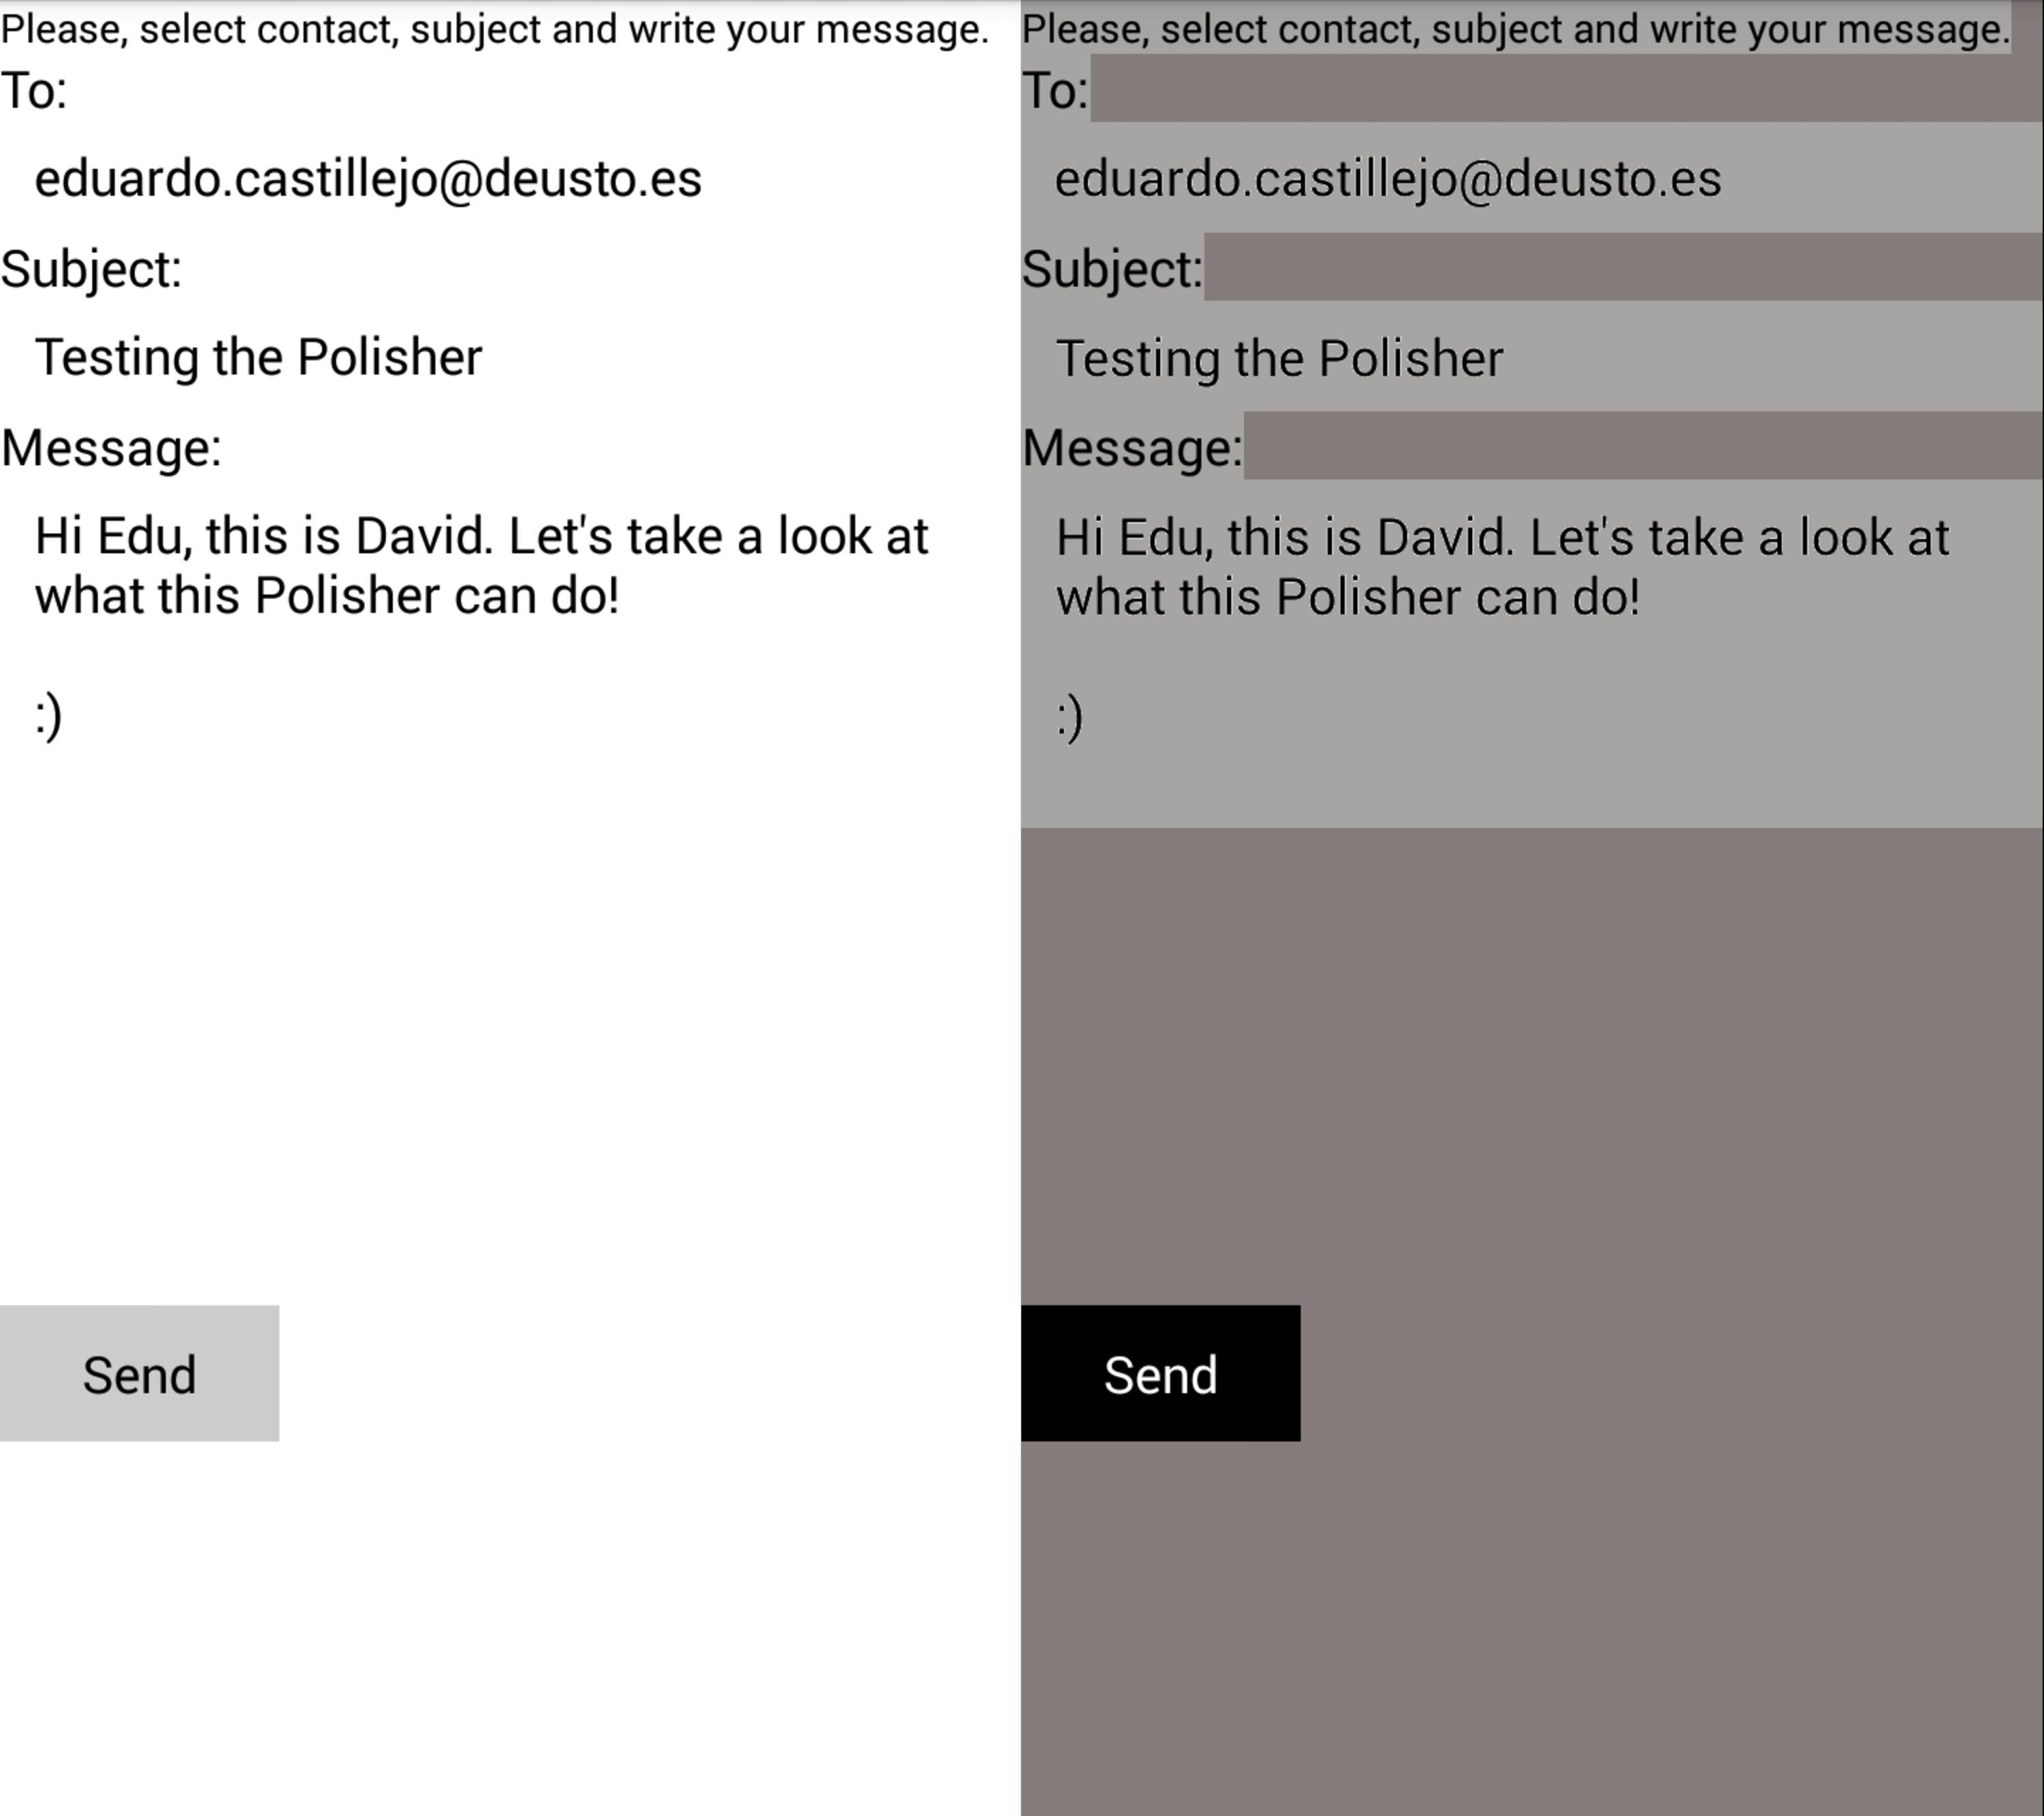
\includegraphics[width=0.65\textwidth]{polisher_scenario.pdf}
\caption{User interface adaptation performed by the Adaptation Engine. On the
left, the default version, without adaptations. On the right, the same 
application adapted by AdaptUI.}
\label{fig:polisher_scenario}
\end{figure}

Thus, David uses his device through the adapted user interface. At this point,
the corresponding interaction model is built by the Adaptation Layer, collecting
the usability metrics shown in Section~\ref{sec:usability_metrics} (see 
Table~\ref{tbl:effectiveness_metrics} and Table~\ref{tbl:productivity_metrics}).
Table~\ref{tbl:model_comparison} shows the used metrics and the computed values
for both the default and the adapted interaction models.

\begin{table}
 \caption{The interaction model computed by the Adaptation Layer. Time ($T$) has
 been measured in seconds.}
 \label{tbl:model_comparison}
 \footnotesize
 \centering
\begin{tabular}{l l l}
  \hline 
  \textbf{Metric} 	& \textbf{Value for the default}& \textbf{Value for the adapted}\\
			& \textbf{interaction model} 	& \textbf{interaction model}	\\
  \hline
  Task effectiveness	& 0.7				& 0.350	\\
  ($M1=|1-\Sigma A_{i}|$)\\
  Task completion	& 1				& 0	\\
  ($X=A/B$)\\
  Error frequency 	& 0.2				& 0.562	\\	%3/15, 18/32 
  ($X=A/T$)\\
  \hline
  Task time		& 15				& 32	\\
  ($X=Ta$)\\
  Task efficiency 	& 0.046				& 0.010	\\
  ($X=M1/T$)\\
%   Productive proportion\\
%   ($X=Ta/Tb$)\\
  Relative user efficiency & 1.0			& 0.5	\\
  ($X=A/B$)\\
  \hline
\end{tabular}
\end{table}

As is shown in Table~\ref{tbl:model_comparison}, the resulting adapted user 
interface provided by AdaptUI does not improve the interaction of the user.
The required time for performing the same task (sending an email) is 32 seconds,
while by default David uses 15 seconds approximately. Thus, the user interface
does not fit the user needs. 

Once the interaction model has been built, the Adaptation Polisher checks the
usability rules set. As detailed in Section~\ref{sec:adaptation_polisher}, these
rules trigger the polisher rules if certain usability ranges are exceeded.
Equation~\ref{ec:usability_rule} shows a usability rule checking the relative
user efficiency of the interaction model.

\footnotesize
\begin{equation} \label{ec:usability_rule}
  \begin{align*} 
  UserAux(?user) \& Productivity(?productivity) \& Polisher(?polisher) \&\\ 
  userAuxHasProductivityMetrics(?user, ?productivity) \& \\
  hasRelativeEfficiency(?productivity, ?efficiency) \& \\
  lessThanOrEqual(?efficiency, 0.5) \& \\
  \Rightarrow \\
  launchPolisherRules(?polisher, true)
  \end{align*}
\end{equation}
\normalsize

On the other hand, Equation~\ref{ec:polisher_rule} is triggered by 
Equation~\ref{ec:usability_rule}. In the consequent of this rule there is 
a value of $1.10$. This value means that the size of the views presented in the
previous adapted version of the user interface should be increased in a $10\%$
Hence, the next rule polishes the adapted user
interface.

\footnotesize
\begin{equation} \label{ec:polisher_rule}
  \begin{align*} 
  Polisher(?polisher) \& launchPolisherRules(?polisher, true) \&\\
  UserAux(?user) \& userAuxHasEffectivenessMetrics(?user, ?effectiveness) \& \\
  effectivenessMetricHasErrorFreequency(?effectiveness, ?freq?) \&\\
  greaterThan(?freq, 0.5)\\
  \Rightarrow \\
  setViewSize(1.10)
  \end{align*}
\end{equation}
\normalsize

Thus, the resulting polished user interface is shown in Figure~\ref{fig:polisher_4}.

\begin{figure}
\centering
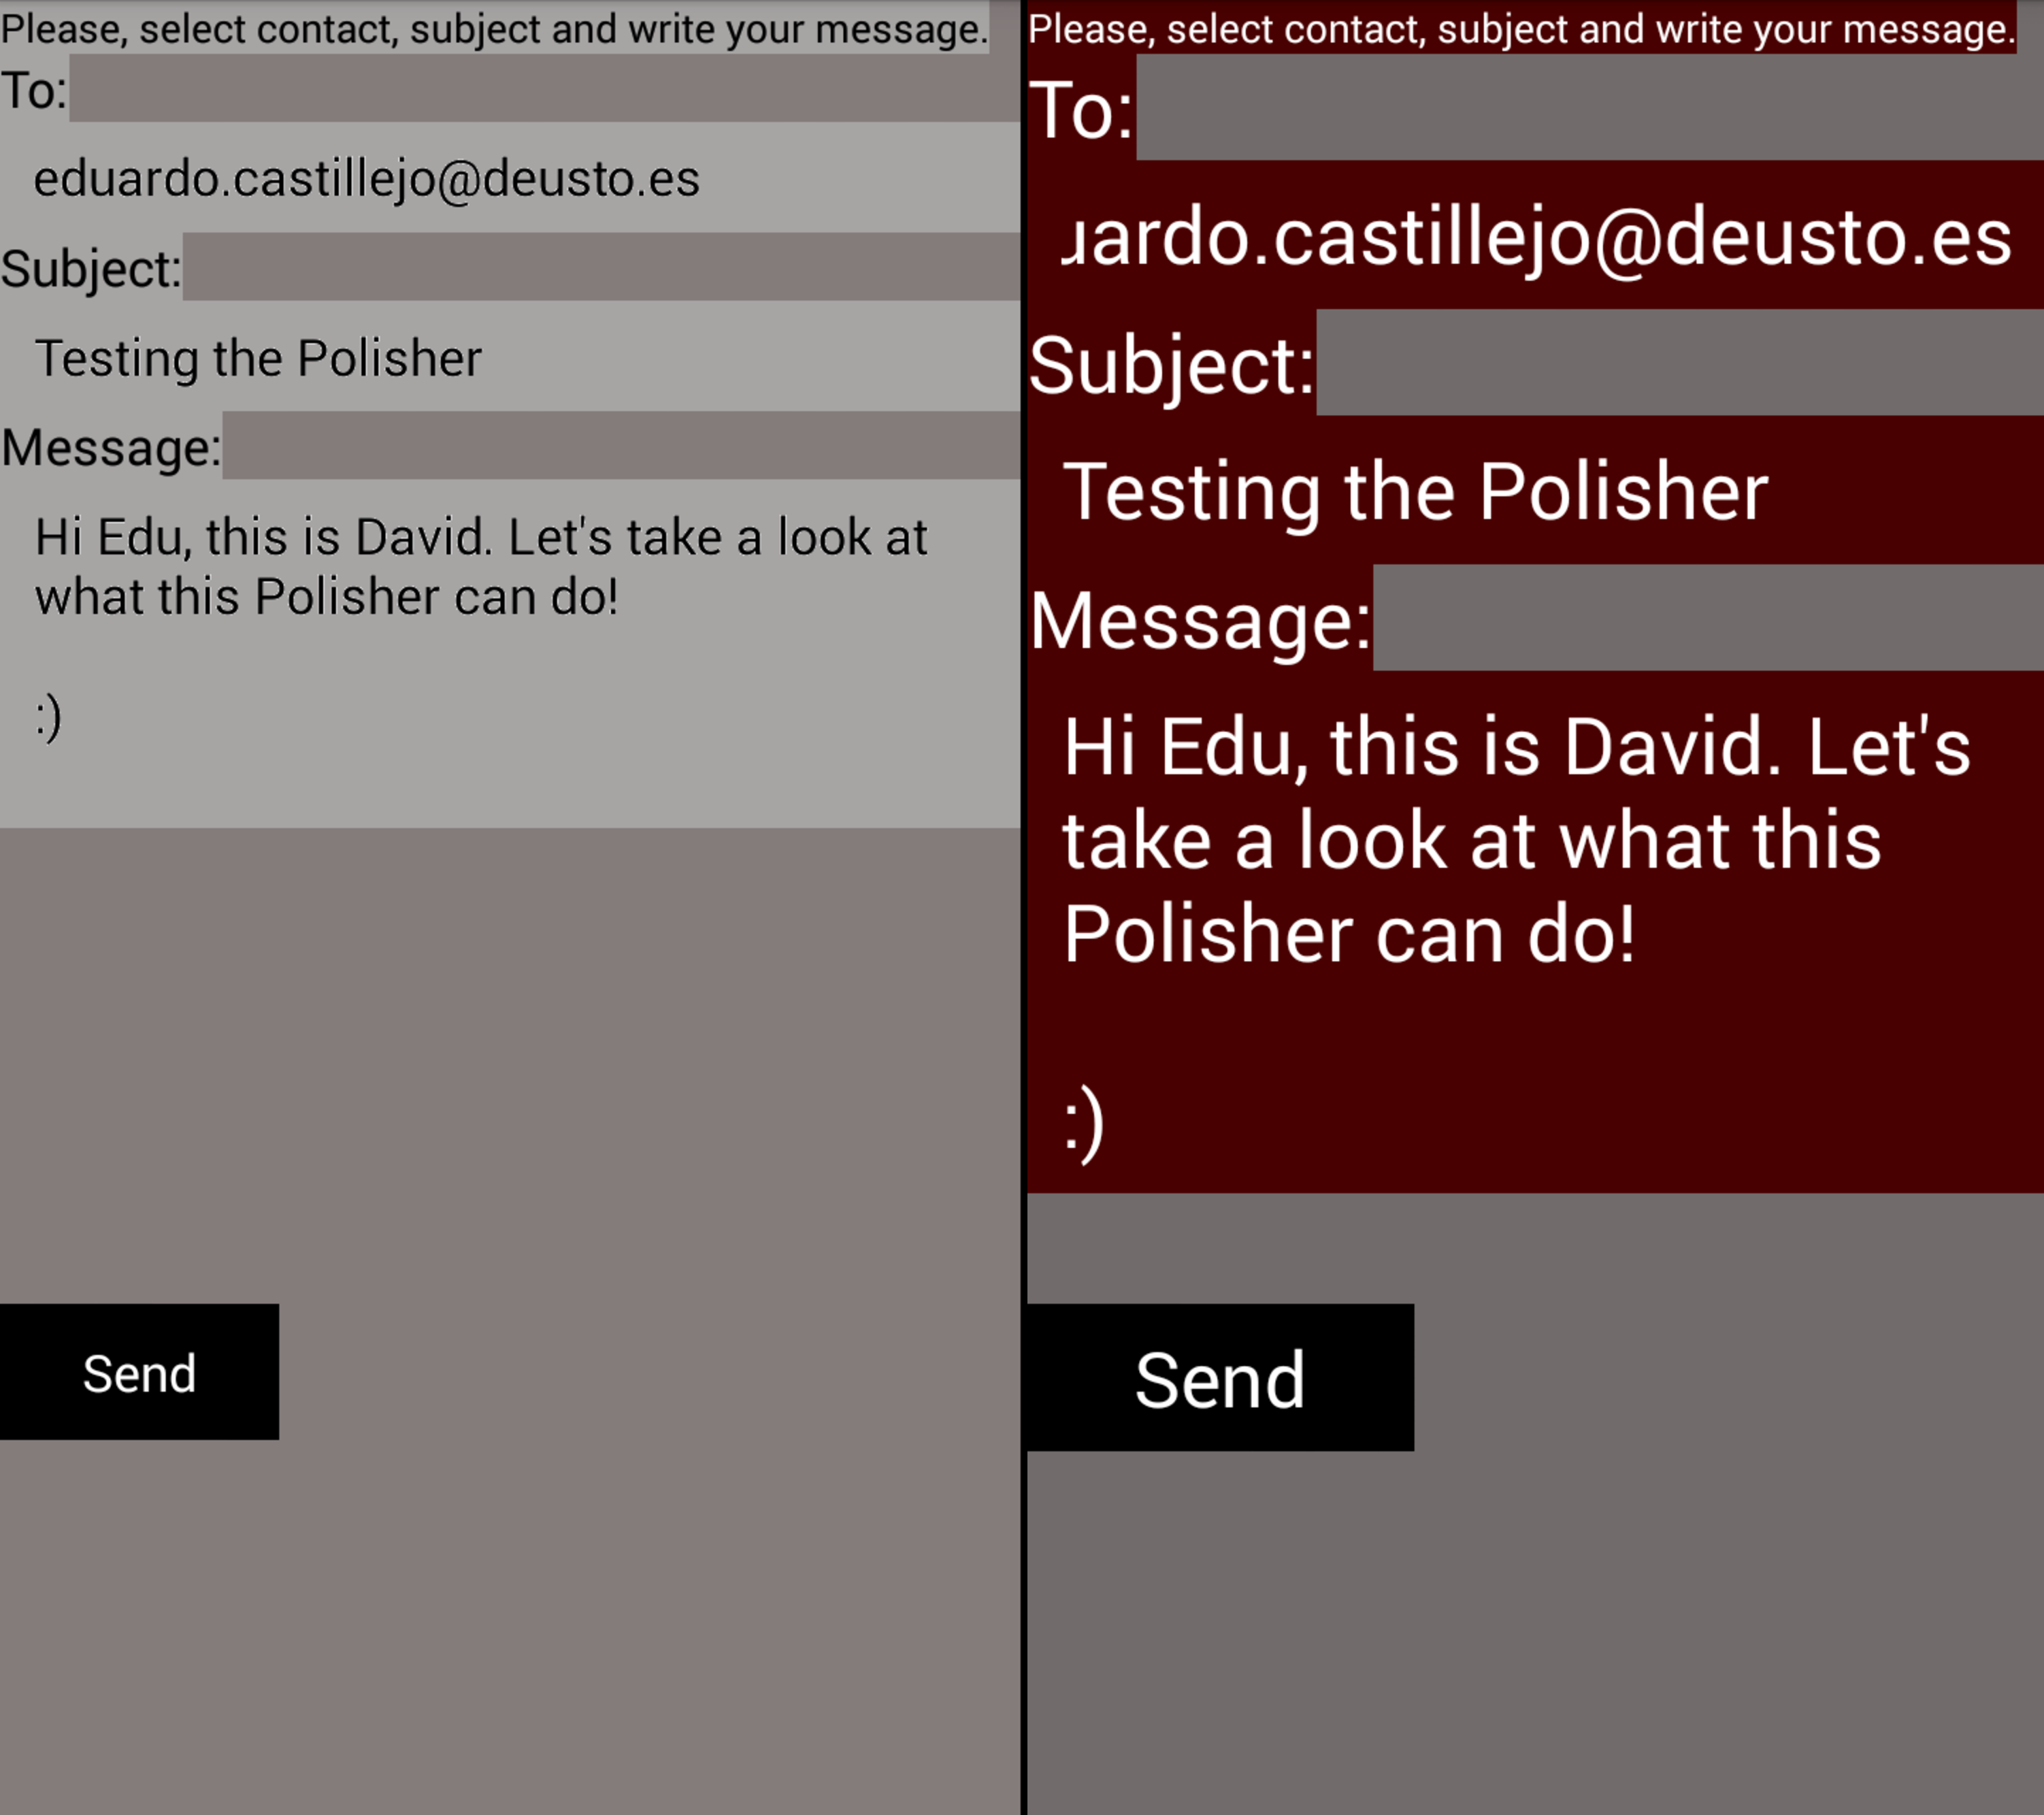
\includegraphics[width=0.65\textwidth]{polisher_4.pdf}
\caption{Polished user interface. On the left, the adapted version. On the 
right, the polished one.}
\label{fig:polisher_4}
\end{figure}
\section{The Application Layer}
\label{sec:application_layer}

The last layer of the AdaptUI architecture is the Application Layer. This layer
aims to ease the use of the AdaptUI platform to developers. To do this, several
tools have been provided. These tools have been designed not only to integrate
AdaptUI within developers' applications (to adapt their user interfaces) but also
to leave in their hands the decision of how to manage the knowledge of the AdaptUI
platform. Thus, through the AdaptUI provided \ac{api}, developers are allowed to:

\begin{enumerate}[label=\alph*)]
 \item Initialize a Pellet reasoner and connect the application to it, loading
 the AdaptUIOnt ontology and its rules.
 
 \item Launch queries about the knowledge stored in the ontology in order to
 adapt the corresponding user interface elements.
 
 \item Generate, change and adapt the knowledge contained in AdaptUI. Classes,
 properties and relationships described in the AdaptUIOnt ontology are fully
 customizable by developers to cover the domain of their adaptation problem.
 
 \item Customize the provided set of rules. The AdaptUI \ac{api} provides a set of
 methods to edit different rules.
\end{enumerate}

The AdaptUI's \ac{api} can be internally divided into two separated \acp{api}. 
The first one, aiming to solve developer's adaptation issues. 
Listing~\ref{lst:api_adaptation} shows an example of an Android activity 
developed using AdaptUI. The second one, with the purpose of adapting the 
knowledge of the domain (see an example in Listing~\ref{lst:api_knowledge}).

\inputminted[linenos=true, fontsize=\footnotesize, frame=lines]{java}{4_system_architecture/api_adaptation.java}
\captionof{listing}{The AbstractActivity class ontology related methods.\label{lst:api_adaptation}}

\inputminted[linenos=true, fontsize=\footnotesize, frame=lines]{java}{4_system_architecture/api_knowledge.java}
\captionof{listing}{Modifying the ontology knowledge with the AdaptUI's \ac{api}.\label{lst:api_knowledge}}


\subsection{The knowledge \ac{api}}
\label{sec:knowledge_api}

Ontologies are formal specification of concepts that represent knowledge within
a specific domain. This knowledge is provided through a vocabulary which describes
the types and relationships of the concepts represented in that specific domain.

The knowledge conceptualization is mainly described through classes, attributes,
relations, individuals and axioms: 

\begin{itemize}
  \item Classes represent concepts within the domain. In other words, classes
  describe the type or kind of the members of the class.
  
  \item Each class can have a set of properties or characteristics which describe
  it. These properties are represented through attributes. These attributes
  are also called datatype properties.
  
  \item Relations detail the relationships that the concepts of the ontology
  might share. They are referred as object properties.
  \item Instances are the representation of the concepts of the
  ontology.
  
  \item Finally, axioms, including rules, are assertions that together comprise
  the overall theory that the ontology describes in the current domain.
\end{itemize}

These concepts together build ontologies to represent the knowledge of a domain.
In AdaptUI,the knowledge of a domain is not considered static. Besides, the 
solutions provided in the literature usually do not apply well when changing 
the domain. Therefore, AdaptUI aims to ease the adaptation of the domain 
knowledge through the customization of these concepts. Through a set of methods 
within the AdaptUI \ac{api}, developers are allowed to insert, edit and delete 
classes, attributes, instances and rules. Table~\ref{tbl:api_knowledge} shows 
the available methods for developers to modify the knowledge contained in the 
AdaptUIOnt ontology.

AdaptUI is designed to support several user capabilities, context status and
device characteristics. Nevertheless, regarding the rules set it is impossible
to assume every possible situation and react accordingly. Thus, a set of methods
to create, edit and delete \ac{swrl} rules has been provided. This allows developers
to adapt the AdaptUI platform to new and unexpected situations in the domain
where the platform might not behave properly.

\begin{center}
\footnotesize

\begin{longtable}{l l l l}
  \caption{Knowledge related AdaptUI \ac{api} methods}\\
  \label{tbl:api_knowledge} \\
% \footnotesize
% \centering
%  \begin{tabular}{l l l l}
  \hline 
  \textbf{\ac{api} group} 	& \textbf{Method name} 	& \textbf{Description} 		& \textbf{Input}\\
  \hline
  Classes		& insertClass		& Inserts a new class.		& The namespace and the \\
			& 			& 				& class name.		\\
			& removeClass		& Erases an existing class, its	& The namespace and the \\
			& 			& individuals, attributes and	& class name.		\\
			& 			& relationships with other 	& 			\\
			& 			& classes.			& 			\\
			& editClass		& Changes the name of the class.& The namespace and the \\
			&			& Internally it deletes the 	& new class name.	\\
			&			& class passed as parameter 	&			\\
			&			& and creates a new one.	&			\\
\hline 
  Object 		& insertObjectProperty	& Inserts a new object property	& The namespace and the	\\
  properties		&			& connecting two classes.	&  object property name.\\
			&			&				& It also needs the 	\\
			& 			& 				& namespaces and names of 	\\
			&			&				& the classes that will be 	\\
			& 			& 				& connected. The two set 	\\ 
			&			&				& of classes are passed as 	\\
			& 			& 				& a Map$<$String namespace,	\\
			& 			& 				& String classname$>$.	\\
			& removeObjectProperty	& Erases an existing datatype	& The namespace and the \\
			& 			& property.			& object property name.	\\
			& editObjectProperty	& Changes the name of the 	& The namespace and the \\
			&			& datatype property. Internally & new class name.	\\
			&			& it deletes the property 	& 			\\
			&			& passed as parameter and 	&			\\
			& 			& creates a new one.		& 			\\
  \hline 
  Datatype 		& addDatatypeProperty	& Inserts a new datatype 	& The namespace and the \\
  properties		&			& property assigning a value to & datatype property name.\\
			& 			& a class.			& 			\\
			&			& If it does not exist, it is	& It also needs the namespace 	\\
			&			& created.			& and name of the class \\
			& 			& 				& that will have this property 	\\
			& 			& 				& and the value type.	\\
			& removeDatatypeProperty& Erases an existing datatype	& The namespace and the \\
			& 			& property.			& datatype property name.\\
			& editDatatypeProperty	& Changes the name of the 	& The namespace and the \\
			&			& datatype property. Internally & new class name.	\\
			&			& it deletes the property passed& 			\\
			&			& as parameter and creates 	&			\\
			& 			& a new one.			& 			\\
  \hline 
  Individuals 		& insertIndividual	& Inserts a new individual of a & The name of the 	\\
			&			& concrete class.		& individual and the 	\\
			& 			& 				& namespace and name 	\\
			& 			& 				& of the class.		\\
			& removeIndividual 	& Removes an individual.	& The name of the 	\\
			&			&				& individual to be 	\\
			& 			& 				& deleted.		\\
  \hline 
  Rules 		& insertRule		& Inserts a new rule.		& The name of the 	\\
			&			& 				& rule, the antecedent 	\\
			& 			& 				& and the consequent.	\\
			& removeRule 		& Removes a rule if the rule 	& The name of the rule 	\\
			&			& has a name associated to it.	& to be deleted.	\\
  \hline
% \end{tabular}
\end{longtable}

\end{center}
\subsection{The adaptation \ac{api}}
\label{sec:adaptation_api}

\section{The Information Flow}
\label{sec:architecture_flow}

Once the AdaptUI's layers and modules have been described, in this section the 
interaction among them and the information flow are reviewed.
Figure~\ref{fig:architecture_flow} shows a diagram with the whole architecture
and data flows.

First, and within the Modelling Layer, the user capabilities and context and
device characteristics are collected by the Capabilities Collector. This module
stores the collected information about these entities in Android using key-value
sets. While the capabilities of the device and several context parameters are
gathered transparently for the user, to collect his/her capabilities the
Capabilities Collector needs the user to complete a profile personalization process.

Once the Capabilities Collector finishes its task, the Semantic Modeller retrieves
the stored information and begins to transform it into semantics using the
AdaptUIOnt ontology. To be able to use semantics and to manipulate the model
and the available knowledge about the entities the Semantic Modeller uses
\textit{Pellet4Android}, which is an Android based port of Pellet.

Next, the Adaptation Engine (within the Adaptation Layer) semantically requests
the last adaptation instructions. These instructions are defined by the rules
triggered when the Semantic Modeller stores the knowledge in the AdaptUIOnt
ontology. Once it is stored, the corresponding rules result into a series of
adaptations. These adaptations, represented through the \textit{Adaptation}
class, are collected by the Adaptation Engine and represented in the user's display.

Once the user receives the corresponding adapted user interface, another Adaptation
Layer's module works in background: the Adaptation Polisher. Actually, this module
starts working from the beginning. Its purpose is to be aware of the user interaction
with the applications. This includes not only the adapted applications but also
the rest of them. Thus, it is able to establish several usability boundaries
under which the user might no be comfortable with. Comparing the user interaction
profile (generated during the usage of default applications under normal
circumstances) and the adapted interaction model (generated during the interaction
with an adapted user interface) this module triggers several instructions to
re-adapt the user interface. These instructions are ruled through the
post-adaptation set of rules.

Finally, within the Application Layer several tools (provided through an \ac{api})
are available for developers to make their applications adaptive and modify the
knowledge which will represent the domain (including concepts, relationships and
rules).

\begin{figure}[H]
\centering
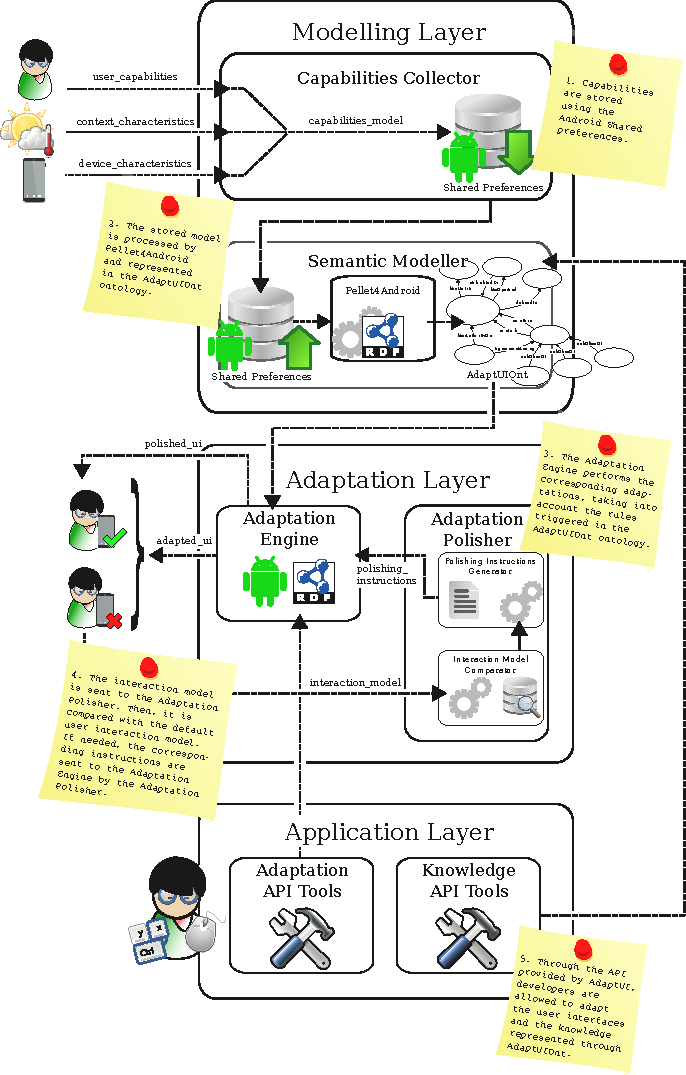
\includegraphics[width=0.85\textwidth]{architecture_flow.pdf}
\caption{The information flow within the AdaptUI platform.}
\label{fig:architecture_flow}
\end{figure}
\section{A Complete Example}
\label{sec:complete_example}

The modules described in the previous sections of this chapter work together to
provide an adapted user interface for the sensed user's context disabilities. 
In the following lines an example of how this process is carried out is 
presented. The definition of the scenario is shown in Table~\ref{tbl:example_scenario}.
% , and the corresponding non adapted user 
% interface is illustrated by Figure~\ref{fig:example_scenario_default}.

\begin{table}[H]
 \caption{Scenario summary.}
 \label{tbl:example_scenario}
 \footnotesize
 \centering
\begin{tabular}{l l}
  \hline 
				& \textbf{Scenario}		\\
  \hline
  User \\
  \qquad - Personal data 	& Molly, $39$ years old, United States\\
  \qquad - Activity	 	& Phone call			\\
  \qquad - Known disabilities 	& - 				\\
% 				& Hearing loss 			\\
%   \hline
  Context \\
  \qquad - Location 		& Relative: Plentzia, Spain  	\\
				& 				\\
  \qquad - Time			& $14$:$35$ 			\\
  \qquad - Brightness		& $30,000$ \ac{lx}		\\
  \qquad - Noise		& $80$ \acp{db}			\\
  \qquad - Temperature		& $28$ ºC 			\\
%   \hline
  Device 			& Samsung Galaxy SII 	 	\\
				& Battery: $55$\%		\\
  \hline
\end{tabular}
\end{table}

The following lines detail the adaptation process, highlighting each layer's and
module's goal and behaviour. As the user is trying to perform a phone call, the 
corresponding default user interface is shown in Figure~\ref{fig:example_scenario_default}.

\begin{figure}[H]
\centering
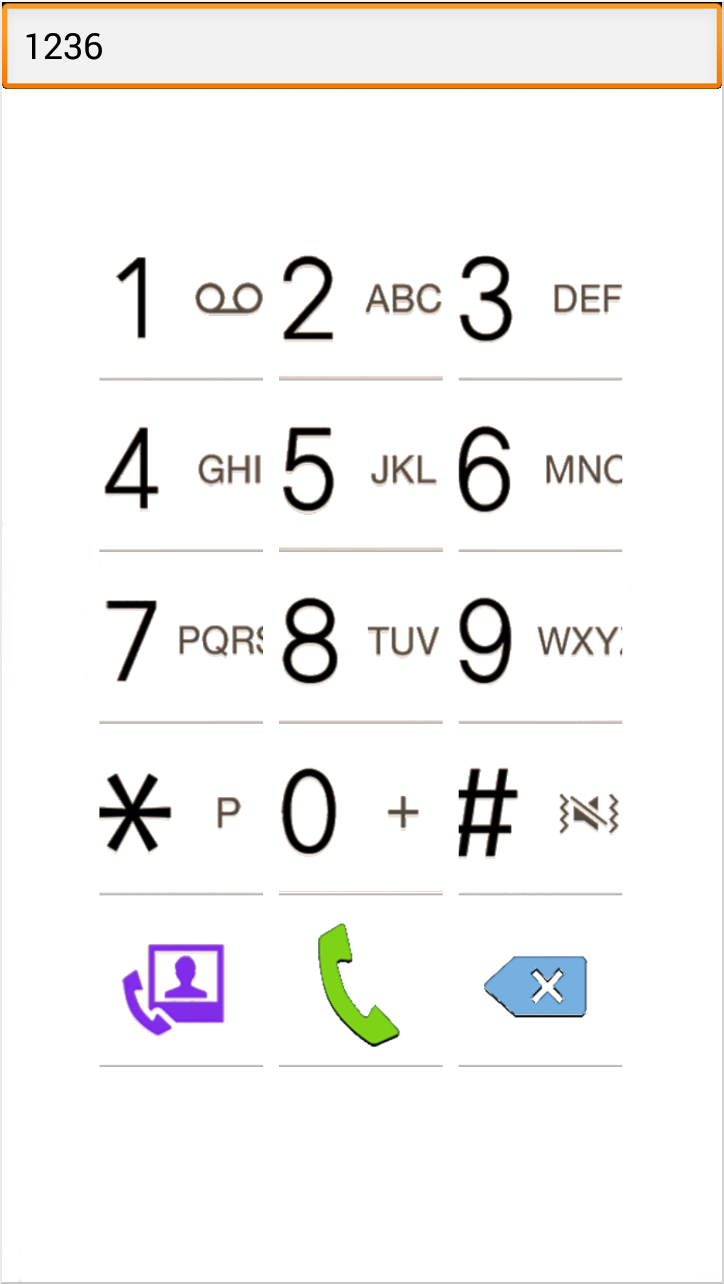
\includegraphics[width=0.35\textwidth]{example_scenario_default.png}
\caption{A simple phone call application user interface.}
\label{fig:example_scenario_default}
\end{figure}

\begin{itemize}
%%%%%%%%%%%%%%%%%%%%%%%%%%%%%%%%%%%%%%%%%%%%%%%%%%%%%%%%%%%%%%%%%%%%%%%%%%%%%%%%
%%%%%%%%%%%%%%%%%%%%%%%%%%Modelling Layer%%%%%%%%%%%%%%%%%%%%%%%%%%%%%%%%%%%%%%%
%%%%%%%%%%%%%%%%%%%%%%%%%%%%%%%%%%%%%%%%%%%%%%%%%%%%%%%%%%%%%%%%%%%%%%%%%%%%%%%%
  \item The Modelling Layer aims to build a semantic model of the user, context
  and device, based on the interaction characteristics available in the current
  situation. For further details of the Modelling Layer see Section~\ref{sec:modelling_layer}.
  
  \begin{itemize}
    %Capabilities Collector%%%%%%%%%%%%%%%%%%%%%%%%%%%%%%%%%%%%%%%%%%%%%%%%%%%%%
    \item First, the user has to use the Capabilities Collector. As explained in 
    Section~\ref{sec:capabilities_collector}, this software module collects non 
    physiological capabilities of the user, gathers different variables of the 
    current context, and identifies several device characteristics. An example of 
    the Capabilities Collector is given through 
    Figure~\ref{fig:capabilities_collector_scenario}. Through a series of
    activities, the user is requested to dynamically configure different user 
    interface components taking into account the current scenario characteristics. 
    Each activity presents different user interface views, and the user's
    interaction decisions are stored in an Android SharedPreferences model.
    This model is easy to maintain and manipulate, and it serves as input for
    the next module. The user, context and device profiles are detailed in 
    Table~\ref{tbl:profiles}.
    
\begin{figure}
\centering
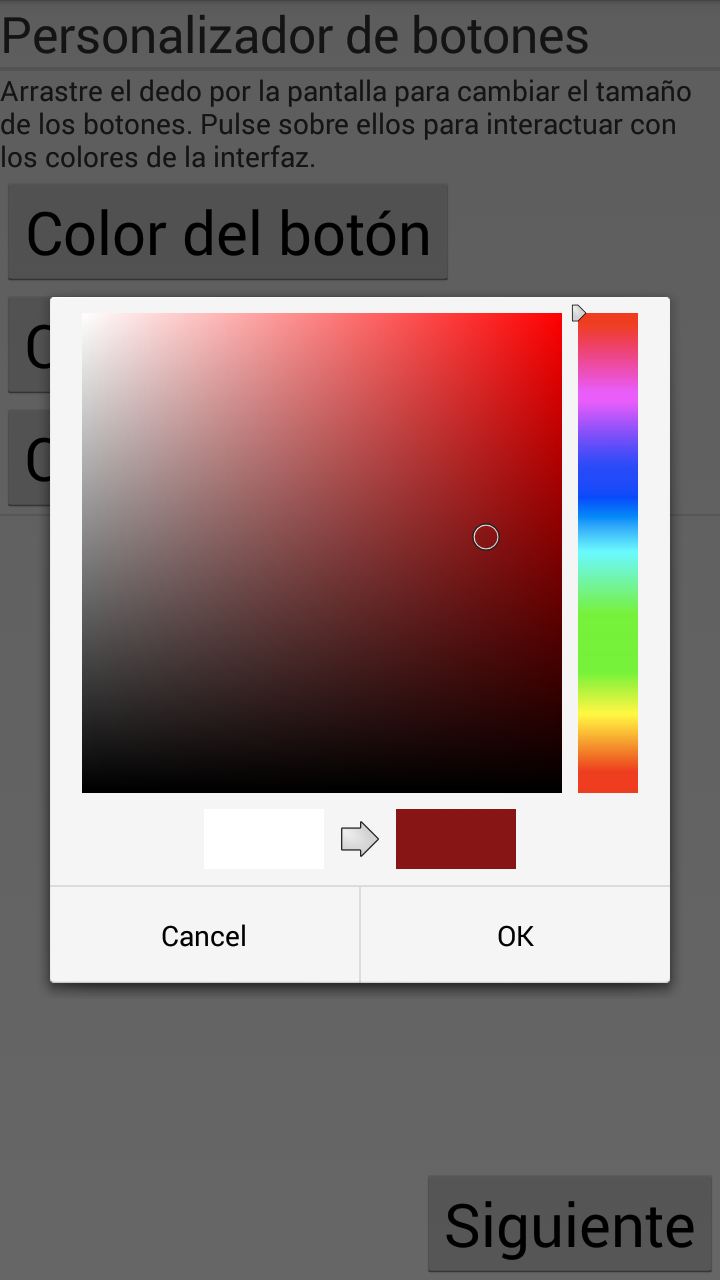
\includegraphics[width=0.35\textwidth]{capabilities_collector_scenario.png}
\caption{A user configuring the buttons colour set through the Capabilities Collector.}
\label{fig:capabilities_collector_scenario}
\end{figure}
    
\begin{table}
 \caption{User, context and device profiles after using the Capabilities Collector.
 The class (*) is translated to a semantic representation in the AdaptUIOnt ontology.
 It is not represented in the SharedPreferences model. The colour set (*) represents
 the whole colour configuration that the user specifies for the corresponding
 views, including the background colours, text colours and so on.}
 \label{tbl:profiles}
 \footnotesize
 \centering
\begin{tabular}{l l l l}
  \hline 
  \textbf{Entity}& \textbf{Class(*)}& \textbf{SharedPreferences} & \textbf{Value}\\
		& 		& \textbf{property} 		& \\
  \hline
  User 		& Interface 	& \textit{input}		& default	\\
		& 		& \textit{output} 		& default	\\
		& View		& \textit{colourSet(*)}		& default	\\
		& Display 	& \textit{minBrightness}	& $9$		\\ 
		& 		& \textit{maxBrightness}	& max		\\
		& Audio 	& \textit{minVolume}		& $4$		\\
		& 		& \textit{maxVolume} 		& max		\\
		& Other 	& \textit{language}		& English	\\
		& 		& \textit{vibration} 		& true 		\\
		
  Context	& Brightness	& \textit{brightness}		& $30,000$	\\
		& Noise		& \textit{noise}		& $80$		\\
		& Time		& \textit{time}			& $14$:$35$	\\
		& Location	& \textit{city}			& Plentzia	\\
		&		& \textit{country}		& Spain		\\
		&		& \textit{longitude}		& $43.414353$	\\
		&		& \textit{latitude} 		& $-2.944183$	\\
  Device	& \ac{os}	& \textit{osVersion}		& $4.1.2$	\\
		& Battery	& \textit{battery}		& $55$		\\
		& Volume	& \textit{maxVolume}		& $12$		\\
		& Brightness	& \textit{maxBrightness}	& $15$		\\
		& DeviceScreenResolution & \textit{resolution}	& $480×800$	\\	
  \hline
\end{tabular}
\end{table}

    %Semantic Modeller%%%%%%%%%%%%%%%%%%%%%%%%%%%%%%%%%%%%%%%%%%%%%%%%%%%%%%%%%%
    \item Once the interaction with the Capabilities Collector is finished, the
    Semantic Modeller (see Section~\ref{sec:semantic_modeller}) uses the 
    SharedPreferences stored model and stores it as a semantic representation of 
    this model in the AdaptUIOnt ontology. This is performed thanks to the 
    \textit{Pellet4Android} mobile semantic engine, which allows to manipulate 
    semantic knowledge in Android. Storing in the ontology requires more time 
    than using SharedPreferences. Thus, the last operation in the Modelling Layer 
    is the semantic storage. The most significant represented characteristics 
    are shown in Table~\ref{tbl:capabilities_collector_scenario}. Those 
    characteristics that are not present in Table~\ref{tbl:profiles} are computed 
    by the pre-adaptation. For example, Equation~\ref{ec:pre_rule_1} updates the 
    \textit{userAuxDisplayHasApplicable} datatype property by checking if the 
    user interacts with the Capabilities Collector in a \textit{default} manner.
    
    \footnotesize
    \begin{equation} \label{ec:pre_rule_1} 
    \begin{align*} 
    adaptui:UserAux(?uaux) ∧ adaptui:UserCharacteristics(?user) ∧ \\
    adaptui:Interface(?interf) ∧ adaptui:Input(?input) ∧ \\
    userHasInterface(?user, ?interf) ∧ interfaceHasInput(?interf, ?input) ∧\\
    swrlb:equal("default") \\    
    \Rightarrow \\
    adaptui:userAuxDisplayHasApplicable(?uaux, true)
    \end{align*}
    \end{equation}
    \normalsize
    
    

  \end{itemize}

\begin{table}
 \caption{User, context and device profiles as represented in the AdaptUIOnt ontology.}
 \label{tbl:capabilities_collector_scenario}
 \footnotesize
 \centering
\begin{tabular}{l l l l}
  \hline 
  \textbf{Entity}& \textbf{Class} & \textbf{Property} 			& \textbf{Value}\\
  \hline
  User 		& Display 	& \textit{userDisplayIsApplicable} 	& true		\\% Esto se saca con reglas
		& 		& \textit{userDisplayBrightnessIsStatic}& false		\\
		& Audio 	& \textit{userDisplayApplicableIsStatic}& false		\\
		& 		& \textit{userAudioHasApplicable} 	& true		\\
		& 		& \textit{userAudioApplicableIsStatic} 	& false		\\
		& 		& \textit{userAudioHasVolume}  		& $4$ 		\\
		& Interface 	& \textit{userInterfaceInput}		& default	\\
		& 		& \textit{userInterfaceOutput} 		& default	\\
% 		& Experience	& \textit{userHasExperience} 		& high		\\
		& View		& \textit{userViewIsStatic}		& false		\\
		& Other 	& \textit{userHasLanguage}		& English	\\
		& 		& \textit{vibration} 			& true 		\\
  Context	& Brightness	& \textit{contextHasBrightness}		& $30,000$	\\
		& Noise		& \textit{contextHasNoise}		& $80$		\\
		& Time		& \textit{contextHasTime}		& $14$:$35$	\\
		& Location	& \textit{contextHasRelativeLocationCity}& Plentzia	\\
		&		& \textit{contextHasRelativeLocationCountry}& Spain	\\
		&		& \textit{contextHasAbsoluteLocationLongitude}& $43.414353$\\
		&		& \textit{contextHasAbsoluteLocationLatitude} & $-2.944183$\\
  Device	& Software (\ac{os})& \textit{deviceHasOSVersion}	& $4.1.2$	\\
		& Hardware (Battery)& \textit{deviceHasBattery}		& $55$		\\
		& (Volume)	& \textit{deviceHasMaxVolume}		& $12$		\\
		& (DeviceScreenResolution) & \textit{deviceHasResolution}& $480×800$	\\	
  \hline
\end{tabular}
\end{table}

%%%%%%%%%%%%%%%%%%%%%%%%%%%%%%%%%%%%%%%%%%%%%%%%%%%%%%%%%%%%%%%%%%%%%%%%%%%%%%%%
%%%%%%%%%%%%%%%%%%%%%%%%%%Adaptation Layer%%%%%%%%%%%%%%%%%%%%%%%%%%%%%%%%%%%%%%
%%%%%%%%%%%%%%%%%%%%%%%%%%%%%%%%%%%%%%%%%%%%%%%%%%%%%%%%%%%%%%%%%%%%%%%%%%%%%%%%
  \item After storing the semantic model in the AdaptUIOnt ontology, it is sent
  to the the Adaptation Layer. This layer aims to lead the dynamic adaptation of
  the elements presented in the user interface.
  
  \begin{itemize}
    %Adaptation Engine%%%%%%%%%%%%%%%%%%%%%%%%%%%%%%%%%%%%%%%%%%%%%%%%%%%%%%%%%%
    \item The Adaptation Engine loads, as input, the stored AdaptUIOnt model, 
    and it executes the corresponding adaptation rules defined by the developer. 
    Once the rules have been executed, the resulting user interface is dynamically 
    updated and presented to the user. Equation~\ref{ec:adap_rule_8} shows how
    the views are updated due to the context brightness. The resulting adapted
    user interface is shown in Figure~\ref{fig:example_scenario_default_vs_adapted}.

    \footnotesize
    \begin{equation} \label{ec:adap_rule_8} 
    \begin{align*} 
    adaptui:Button(?b) ∧ adaptui:ContextCharacteristics(?c) ∧ gumo:Light(?light) ∧ \\  
    gumo:PhysicalEnvironment(?pe) ∧ contextHasPhysicalEnvironment(?c, ?pe) ∧ \\ 
    lightHasBrightness(?light, ?value) ∧ physicalEnvironmentHasLight(?pe, ?light) ∧ \\
    swrlb:greaterThanOrEqual(?value, 20000) \\
    \Rightarrow \\
    adaptui:buttonHasBackgroundColor(?b, -16711936)
    \end{align*}
    \end{equation}
    \normalsize
    
    \begin{figure}
    \centering
    \includegraphics[width=0.50\textwidth]{example_scenario_default_vs_adapted.png}
    \caption{The default user interface (left) and the adapted user interface (right).}
    \label{fig:example_scenario_default_vs_adapted}
    \end{figure}
    
    %Adaptation Polisher%%%%%%%%%%%%%%%%%%%%%%%%%%%%%%%%%%%%%%%%%%%%%%%%%%%%%%%%
    \item Finally, the Adaptation Polisher monitors the usability of the adapted
    user interface. To safeguard this usability it builds and compares two
    interaction models. The first one is built with the usability metrics detailed
    in Section~\ref{sec:usability_metrics} under default circumstances. This means
    that this model is fully accessible by the user in many contexts. The second 
    model, is built from the same usability metrics but taking into account the 
    adapted user interface. The Interaction Model Comparator executes the following
    interaction rules, which aim to evaluate the usability metrics differences
    between the two interaction models. Once these rules are executed, their
    results update the last adaptation of the user interface if needed. The
    polished user interface is compared with the adapted one in 
    Figure~\ref{fig:example_scenario_adapted_vs_polished}. In the presented
    scenario, the Equation~\ref{ec:pre_rule_8} updates polishes the button's
    text as follows: 

    \footnotesize
    \begin{equation} \label{ec:pre_rule_8} 
    \begin{align*} 
    adaptui:Button(?b) ∧ adaptui:Usability (?u) ∧ adaptui:EfficiencyMetric(?em) ∧ \\
    usabilityHasEfficiencyMetric(?u, ?em) ∧ swrlb:greaterThanOrEqual(?value, 0.5) ∧ \\
    efficiencyMetricHasTaskEffectiveness(?em, ?value)\\
    \Rightarrow \\
    adaptui:buttonHasTextColor(?b, 16777215)
    \end{align*}
    \end{equation}
    \normalsize

    \begin{figure}
    \centering
    \includegraphics[width=0.50\textwidth]{example_scenario_adapted_vs_polished.png}
    \caption{The adapted user interface (left) and the polished user interface (right).}
    \label{fig:example_scenario_adapted_vs_polished}
    \end{figure}

  \end{itemize}

\end{itemize}

As this example demonstrates, the polisher rules allow the developer to keep
improving the adapted user interfaces. This is carried out by maintaining both
default and adapted interaction models which are based on the usability metrics
detailed in Section~\ref{sec:usability_metrics}.

% Modelling Layer
% - Capabilities Collector
% 1. Llegan las capacidades.
% 2. Se genera el modelo.
% 3. Se guarda en formato SharedPreferences.
% - Semantic Layer
% 4. Se guarda en formato semántico.
% 
% Adaptation Layer
% - Adaptation Engine
% 1. Se analiza el modelo semántico.
% 2. Se ejecutan las reglas correspondientes.
% 3. Se actualiza la interfaz con la nueva adaptación resultante.
% - Adaptation Polisher
% 1. Se genera el modelo de interacción.
% 2. Se ejecutan las reglas de interacción.
% 3. Se envían los resultados al Polishing instructions Generator.
% 4. Se ejecutan las reglas de polishing.
% 5. Se envía al Adaptation Engine la interfaz a adaptar.

%: ----------------------- introduction file header -----------------------
\begin{savequote}[50mm]
So you see, the only proof of what you are is in the way you hear the truth.
% Don't be scared, live to win, although they're always gonna tell you it's a sin.
\qauthor{Motörhead - Stay Clean}
\end{savequote}

% the code below specifies where the figures are stored
\ifpdf
\graphicspath{{5_experiments_and_results/figures/PNG/}
{5_experiments_and_results/figures/PDF/}{5_experiments_and_results/figures/}}
\fi

\chapter{Evaluation}
\label{cha:evaluation}
%------------------------------------------------------------------------- 

% INTRODUCTION OF THE CHAPTER

In the previous chapters several contributions have been presented. All these
contributions together define AdaptUI, a mobile platform which regards adaptive 
and dynamic user interfacing for mobile devices. AdaptUI combines mobile 
semantics and reasoning, supported by an ontology which models user's 
characteristics, context current conditions and device's hardware and software 
characteristics. In this chapter an evaluation of the designed ontology and the 
semantic based platform which manages it is performed. This evaluation is 
addressed through several experiments, regarding cycle time responsiveness, 
system performance with specific operations (e.g., reasoning over a controlled 
set of rules), other alternatives and, finally, analysing users' acceptance and 
feedback.

Consequently, this chapter is divided in two different parts considering the 
experiments' goals. On the one hand, an evaluation of the technical performance
of the AdaptUI system is presented. Including quantitative and qualitative 
experiments, this technical evaluation has been developed as follows:

\begin{enumerate}[label=\alph*)]
  \item First, the developed mobile adaptation of the Pellet reasoning engine 
  is tested through several scenarios. In these scenarios different   
  modifications of the AdaptUIOnt ontology are presented in order to evaluate 
  the performance differences of \textit{Pellet4Android} and Pellet.
  
  \item Next, as the system goal is to adapt the user interface, a comparison 
  with another user interface adaptation solution has been performed: the 
  Imhotep framework. Imhotep is a user interface adaptation framework which 
  aims to ease the development of adaptable and more accessible user 
  interfaces.
  
  \item Finally, several scenarios are presented in which the adaptation process
  of the AdaptUI system is described step by step, from the scenario conditions
  to the adaptation results. These scenarios have been divided into three 
  different groups, each group aiming to cover different types of adaptation 
  and environments. This classification includes:
  \begin{itemize}
    \item A scenario in which the limitations suffered by the user are caused
    by the current context conditions. 
    
    \item A second scenario introducing several limitations due to the  
    activities the user performs.
    
    \item A final case in which several disabilities impedes the user to 
    interact properly with the user interface.
  \end{itemize}
\end{enumerate}

On the other hand, an evaluation regarding users, without technical knowledge
requisites, is performed. This part of the evaluation is based on the user
satisfaction when using AdaptUI. The scenario for this experiment includes the
user and an Android based tutorial through which the user indicates several 
interaction parameters. Taking into account different context situations, 
several applications are adapted consequently. After the adaptation, the user 
is asked to complete a questionnaire of usability. More concretely, the \ac{sus} 
questionnaire is presented (among several extra questions to classify the 
results).

Hence, the the reminder of this chapter has been structured as follows: 

\begin{itemize}
  \item A technical evaluation, which experiments are detailed in 
  Section~\ref{sec:technical_evaluation}. These experiments regard the 
  reasoning performance comparing Pellet for desktop versus Pellet for mobile 
  devices. The provided \acp{api} have been also evaluated in an experiment
  including developers.
  
  \item A usability evaluation of the system, which details are accordingly 
  described in Section~\ref{sec:user_evaluation}. This evaluation includes 
  users interacting with the AdaptUI system. In order to evaluate the usability 
  of AdaptUI a usability questionnaire is presented to the users. 
  Section~\ref{sec:sus_results} presents Table~\ref{tbl:additional_questions} and
  Table~\ref{tbl:sus_questionnaire_results}, which shows the responses from all
  the users participating in the evaluation of AdaptUI.

  \item Finally, Section~\ref{sec:evaluation_discussion} and 
  Section~\ref{sec:evaluation_conclusions} summarize and analyse the results
  obtained and detailed in the previous sections, regarding both technical and
  usability aspects.
\end{itemize}

\section{Technical Evaluation}
\label{sec:technical_evaluation}

The technical evaluation of this chapter includes several experiments that are 
carried out aiming to test the performance of the adaptation process. One of 
the most important developed modules of AdaptUI is the Pellet reasoning 
engine port for Android. This module requires special emphasis in the evaluation, 
as leads the whole adaptation process. Besides, several other experiments are 
presented. Thus, in the following sections these experiments and their results 
are detailed:

% This section gathers several experiments regarding the technical part of the 
% evaluation. Within this section the following experiments are included:

\begin{enumerate}[label=\alph*)]
  \item First, Section~\ref{sec:performance_evaluation} presents a series 
  of experiments regarding the performance of \textit{Pellet4Android} in 
  comparison with Pellet for Java. These experiments include the default
  AdaptUIOnt ontology and different versions of AdaptUIOnt with several modifications
  of the axioms sets. For more details of the \textit{Pellet4Android} mobile 
  reasoning engine see Section~\ref{sec:pellet4android}.
  
  \item Second, AdaptUI is compared to another user adaptation solution: 
  Imhotep. This is detailed in Section~\ref{sec:imhotep_comparison}.
  
  \item Next, several scenarios are presented to evaluate the adaptation 
  process of AdaptUI. Besides, a comparison with Imhotep user adaptation 
  framework is also performed. The scenarios and their details are given in 
  Section~\ref{sec:scenarios}.
  
  \item Finally, $5$ developers with experience in developing Android based 
  applications have evaluated the provided \acs{api}. This experiment is detailed
  in Section~\ref{sec:developers}.
\end{enumerate}


\subsection{Performance Evaluation for Pellet and Pellet4Android}
\label{sec:performance_evaluation}

During this section different experiments are presented in order to 
discuss the results of using mobile reasoning engines. In our case we evaluate 
the reasoning performance of \textit{Pellet4Android}, the Android based version 
of Pellet ported for AdaptUI. To do so, this evaluation considers Pellet, the 
desktop Java based reasoning engine, to make a comparison between the 
performance results of both solutions. This evaluation has been divided into 
three different experiments:

\begin{enumerate}
  \item The first experiment consists in using the default AdaptUIOnt ontology 
  version with both reasoning engines. When loading the ontology several rules 
  are processed and triggered. As a result of this experiment the  
  corresponding performance results are compared.
  
  \item For the second experiment the ABox axioms set of the AdaptUIOnt 
  ontology is increased. The ABox gathers the knowledge about the 
  individuals, including concepts and roles assertions, and individuals 
  equality and inequality~\citep{krotzsch_description_2012}. In other words, 
  it describes the attributes of instances (or individuals), the roles between 
  instances, and other assertions about instances regarding their class 
  membership with the TBox concepts~\citep{abox_tbox}. The ABox, RBox and TBox 
  belong to the \ac{owl} 2 Description Logic (DL). As for these experiments several 
  modifications have been carried out in these axiom sets, a more concrete 
  description of the concepts represented by each set is detailed in 
  Table~\ref{tbl:dl_terminology}. Hence, increasing the number of individuals   
  might result into difference performance results comparing both platforms.
  
  \item Next, the \ac{swrl} axioms set of the AdaptUIOnt ontology is modified by 
  increasing its axioms. This axiom set collects axioms related to the rules 
  included in the ontology. Therefore, this experiment focuses on the reasoning 
  capabilities of each version of Pellet.
\end{enumerate}

\begin{table}
 \caption{TBox and ABox components purposes~\citep{abox_tbox}.}
 \label{tbl:dl_terminology}
 \footnotesize
 \centering
\begin{tabular}{l l l}
  \hline 
  \textbf{ABox} 				&  \textbf{TBox} \\
  \hline 
  Membership assertions, either as concepts or  & Definitions of the concepts and properties of the 	\\
  as roles. 					& controlled vocabulary.				\\
  Attributes assertions. 			& Declarations of concept axioms or roles.		\\
  Linkages assertions that capture the above	& Inferencing of relationships, be they transitive, 	\\
  but also assert the external sources for 	& symmetric, functional or inverse to another 		\\
  these assignments. 				& property.						\\
  Consistency checking of instances.		& Equivalence testing as to whether two classes or 	\\
  Satisfiability checks, which imply that the	& properties are equivalent to one another.		\\
  conditions of instance memberships are met.	& Subsumption, which is checking whether one 		\\
						& concept is more general than another.			\\
						& Satisfiability, which is the problem of checking 	\\
						& whether a concept has been defined (is not an 	\\
						& empty concept).					\\
						& Classification, which places a new concept in  	\\
						& the proper place in a taxonomic hierarchy of 		\\
						& concepts.						\\
						& Logical implication, which is whether a generic 	\\
						& relationship is a logical consequence of the		\\ 
						& declarations in the TBox.				\\
						& Infer property assertions implicit through the 	\\
						& transitive property.					\\	
\hline
\end{tabular}
\end{table}

% For these experiments several tables and the corresponding charts are included,
% showing the results obtained during the tests. In these tables the ontology 
% triples, ABox and \ac{swrl} axioms sets, mean, median and deviation are shown. The
% triples are obtained by a SPARQL query (see Listing~\ref{lst:fuseki}). On the
% other hand the axioms are requested through the \ac{owl}-API.
% 
% \lstset{label=lst:fuseki, language=java, basicstyle=\footnotesize, frame=single,
% keywordstyle=\color{blue}, captionpos=b, caption={SPARQL query for obtaining the
% number of triples of the ontology. Between the $WHERE$ braces there is:
% $?s$, which represents the subject; $?p$, representing the predicate; and $?o$,
% which represents the object.}, breakatwhitespace=false, breaklines=true}
% \begin{lstlisting}
%   SELECT (COUNT(*) AS ?no) WHERE { ?s ?p ?o  }
% \end{lstlisting}


The cited experiments have been performed using two different types of devices 
have been used. The ones running Pellet have been launched using a desktop 
environment. On the contrary, as \textit{Pellet4Android} is an Android based 
version of the reasoning engine, several mobile devices have been tested. The 
characteristics of all the devices used for these experiments are detailed in 
Table~\ref{tbl:devices_specs}. 

\begin{table}
 \caption{Execution platforms software and hardware main specifications. The \ac{ram}
 memory is measured in \ac{gb} and the \ac{cpu} processor in \ac{ghz}.}
 \label{tbl:devices_specs}
 \footnotesize
 \centering
\begin{tabular}{l l l l}
  \hline 
 \textbf{Device} 		& \multicolumn{2}{c}{\textbf{Hardware}} 	
& \textbf{Software}	\\
				& \textbf{\ac{ram}} & \textbf{\ac{cpu}} 			
& \textbf{\ac{os}} 		\\
    \hline 
  Acer TravelMate 8481  	& 8.0	& Quad-core 1.60 Intel® 	 	
& Ubuntu 13.10 		\\
				& 	& Core™ i5-2467M			
& (64 bits)		\\
  Samsung Galaxy SIII Mini	& 1.0 	& Dual-core 1.0, Cortex-A9	 	
& Android 4.1.2 	\\
  Samsung Galaxy SIII 		& 1.0 	& Quad-core 1.4, Cortex-A9 		
& Android 4.3   	\\
  Samsung Nexus 10 		& 2.0 	& Dual-core 1.7, Cortex-A15 		
& Android 4.4.2 	\\
\hline
\end{tabular}
\end{table}

The mobile devices shown in the previous table have not been chosen arbitrarily.
As can be seen in Figure~\ref{fig:android_market}, at February 2014 the global
spread of Samsung devices represent the 65\% share of all Android devices.

\begin{figure}
\centering
\includegraphics[width=0.75\textwidth]{android_market.pdf}
\caption{Global Android share~\citep{samsung_share_2014}. As this pie chart
illustrates, Samsung devices represent the 65\% of the Android worldwide market
share.}
\label{fig:android_market}
\end{figure}

According to the explanation of this section, in the following lines each 
experiment is described and evaluated. First, the default AdaptUIOnt reasoning 
performance comparing Pellet and \textit{Pellet4Android} is introduced in 
Section~\ref{sec:eval_default_ont}. Next, these reasoning engines are 
tested using a modification of the default ontology, increasing the ABox axioms 
set. This experiment is described in Section~\ref{sec:eval_abox}. 
Finally, the AdaptUIOnt default ontology's \ac{swrl} axioms set is increased to 
evaluate the performance of both reasoning engines when dealing with larger 
sets of rules (see Section~\ref{sec:eval_swrl}).


\subsubsection{Using the Default AdaptUIOnt Ontology}
\label{sec:eval_default_ont}

In this experiment the default version of the AdaptUIOnt ontology is used as 
input of the reasoning engines in order to evaluate their performance. As 
AdaptUIOnt has been designed to be a light ontology to be available to be used 
with mobile reasoning engines, this experiment shows how \textit{Pellet4Android} 
performs in comparison with the the results obtained by Pellet in a desktop 
environment. These results are shown in Table~\ref{tbl:eval_default_ont}.

\begin{table}
 \caption{Pellet and \textit{Pellet4Android} comparison loading the default 
AdaptUIOnt ontology.}
 \label{tbl:eval_default_ont}
 \footnotesize
 \centering
  \begin{tabular}{l l r r r r r r}
  \hline 
  &  & \multicolumn{2}{c}{\textbf{Axioms}} & 
  \multicolumn{3}{c}{\textbf{Results}}	\\
  \textbf{Device} & \textbf{Triples}& \textbf{ABox} & \textbf{\ac{swrl}}
  & \textbf{Mean} & \textbf{Median} & \textbf{Deviation}	\\
  \hline 
  Acer laptop	& 2,779	& 37  & 13 & 0.946 & 0.951 & 0.017	\\
  (Pellet)							\\
  Galaxy SIII Mini& 2,779& 37 & 13 & 2.764 & 2.737 & 0.127	\\
  (\textit{Pellet4Android})					\\
  Galaxy SIII	& 2,779	& 37  & 13 & 1.649 & 1.652 & 0.076	\\
  (\textit{Pellet4Android})					\\
  Nexus 10	& 2,779	& 37  & 13 & 5.147 & 5.122 & 0.205	\\
  (\textit{Pellet4Android})					\\
  \hline
\end{tabular}
\end{table}

Figure~\ref{fig:pellet_default} illustrates the differences of using Pellet or
\textit{Pellet4Android} when loading the default ABox and \ac{swrl} axiom sets in 
AdaptUIOnt. As is shown in Figure~\ref{fig:pellet_default} and in 
Table~\ref{tbl:eval_default_ont}, the performance of Pellet for Java 
environments is better in any case if we compare it with the Android based 
version. However, and although there are several differences depending on the 
used mobile device, the differences are small. This is specially remarkable in 
the case of the Samsung Galaxy SIII. This device performs a remarkable 1.649 
seconds, which is just approximately 0.7 slower than Pellet for Java.

\begin{figure}
\centering
\includegraphics[width=0.75\textwidth]{pellet_default.pdf}
\caption{Pellet and \textit{Pellet4Android} performance comparison using the
default AdaptUIOnt ontology.}
\label{fig:pellet_default}
\end{figure}

\subsubsection{Incrementing the ABox Axioms Set}
\label{sec:eval_abox}

In this case the experiment consists in incrementing the ABox axioms set of 
the AdaptUIOnt ontology. As stated before, the ABox describes the attributes of 
instances, the roles between instances, and other assertions about instances 
regarding their class membership with the TBox concepts~\citep{abox_tbox}. 
The modification of the ABox has been carried out by incrementing the amount of 
instances in 5,000, 10,000, 15,000 and finally reaching 20,000 instances. Thus, 
with this experiment we want to evaluate how increasing the number of 
individuals might result into a performance penalization, specially in the case 
of \textit{Pellet4Android}. Table~\ref{tbl:eval_abox} shows the results of this
experiment.

\begin{table}
 \caption{Pellet and \textit{Pellet4Android} comparison loading the AdaptUIOnt 
ontology with an increment in the ABox axiom set.}
 \label{tbl:eval_abox}
 \footnotesize
 \centering
  \begin{tabular}{l l r r r r r r}
  \hline 
  &  & \multicolumn{2}{c}{\textbf{Axioms}} & 
  \multicolumn{3}{c}{\textbf{Results}}	\\
  \textbf{Device} & \textbf{Triples}& \textbf{ABox} & \textbf{\ac{swrl}}
  & \textbf{Mean} & \textbf{Median} & \textbf{Deviation}	\\
  \hline 
  Acer laptop & 12,779 & 5,000  & 13 & 3.014 & 3.012 & 0.034	\\  
  (Pellet)    & 22,779 & 10,000 & 13 & 3.903 & 3.905 & 0.052	\\
	      & 32,779 & 15,000	& 13 & 4.228 & 4.231 & 0.036	\\
	      & 42,779 & 20,000 & 13 & 4.539 & 4.541 & 0.042	\\
  \hline	      
  Galaxy SIII Mini& 12,779& 5,000& 13& 59.412& 59.508& 0.708	\\
  (\textit{Pellet4Android}) & 22,779 & 10,000 & 13 & 30.321 & 30.327 & 0.347 \\
	      & 32,779 & 15,000	& 13 & 87.957 & 87.018 & 1.108 	\\
	      & 42,779 & 20,000	& 13 & 183.882&183.879 & 2.101	\\
  \hline	      
  Galaxy SIII & 12,779 & 5,000	& 13 & 36.336 & 36.194 & 0.668	\\
(\textit{Pellet4Android})& 22,779 & 10,000 & 13	& 16.471 & 16.439 & 0.288\\
		& 32,779 & 15,000 & 13 & 45.387	& 45.593 & 0.729\\
		& 42,779 & 20,000 & 13 & 97.151	& 97.440 & 1.120\\
  \hline		
  Nexus 10	& 12,779 & 5,000  & 13 & 14.171 & 14.428 & 0.525\\
(\textit{Pellet4Android})& 22,779 & 10,000 & 13 & 9.024 & 9.065 & 0.291\\
		& 32,779 & 15,000 & 13 & 17.944& 17.969  & 0.496\\
		& 42,779 & 20,000 & 13 & 32.070	& 32.019 & 0.588\\
  \hline
\end{tabular}
\end{table}

Figure~\ref{fig:pellet_abox} illustrates the differences between Pellet and
\textit{Pellet4Android} when loading the AdaptUIOnt ontology with an increment 
applied to the ABox axioms set. As is shown in the chart (accordingly with
Table~\ref{tbl:eval_abox}) the performance of Pellet for Java environments 
keeps being better in comparison with the Android based version. While Pellet
maintains its performance under 5 seconds, Android devices require much more
time to perform the same reasoning. In fact, specially the Samsung Galaxy SIII 
Mini mobile device requires more than 180 seconds to evaluate the corresponding
20,000 instances, while the Samsung Galaxy SIII needs approximately 97 seconds 
and the Nexus 10 not more than 32.

\begin{figure}
\centering
\includegraphics[width=0.95\textwidth]{pellet_abox.pdf}
\caption{Pellet and \textit{Pellet4Android} performance comparison using the
AdaptUIOnt ontology increasing the ABox axioms set.}
\label{fig:pellet_abox}
\end{figure}

\subsubsection{Incrementing the \ac{swrl} Axioms Set}
\label{sec:eval_swrl}

Finally, this last experiment consists in incrementing the \ac{swrl} axioms set of 
the AdaptUIOnt ontology, which collects the axioms related to the rules
included in the ontology. Using an amount of 5,000, 10,000, 15,000 and 
finally 20,000 rules we aim to evaluate how increasing the number of rules 
penalize the performance of Pellet, specially in the case of 
\textit{Pellet4Android}. Table~\ref{tbl:eval_swrl} shows the results of this
experiment.

\begin{table}
 \caption{Pellet and \textit{Pellet4Android} comparison loading the AdaptUIOnt 
ontology with an increment in the \ac{swrl} axiom set.}
 \label{tbl:eval_swrl}
 \footnotesize
 \centering
  \begin{tabular}{l l r r r r r r}
  \hline 
  &  & \multicolumn{2}{c}{\textbf{Axioms}} & 
  \multicolumn{3}{c}{\textbf{Results}}	\\
  \textbf{Device} & \textbf{Triples}& \textbf{ABox} & \textbf{\ac{swrl}}
  & \textbf{Mean} & \textbf{Median} & \textbf{Deviation}	\\
  \hline 
  Acer laptop & 82,779  & 37 & 5,013  & 4.770 & 4.732 & 0.141	\\
  (Pellet)    & 162,779 & 37 & 10,013 & 6.327 & 6.296 & 0.164 	\\
	      & 242,779	& 37 & 15,013 & 7.427 & 7.194 & 0.444 	\\
	      & 322,779	& 37 & 20,013 & 8.147 & 8.117 & 0.105	\\
  \hline
 Galaxy SIII Mini& 82,779 & 37 & 5,013  & 96.878  & 96.988  & 0.109 \\
(\textit{Pellet4Android}) & 162,779& 37 & 10,013 & 101.656 & 101.899 & 0.322 \\
	      & 242,779	& 37 & 15,013 & 243.981	& 244.011 & 0.298 \\
	      & 322,779	& 37 & 20,013 & 331.433	& 331.894 & 0.110 \\	
	\hline      
  Galaxy SIII & 82,779	& 37 & 5,013 & 84.121 & 84.121 & 0.869	\\
(\textit{Pellet4Android})& 162,779 & 37	& 10,013 & 74.248 & 74.103 & 0.250\\
		& 242,779 & 37 & 15,013	& 209.431 & 208.628 & 1.699 \\
		& 322,779 & 37 & 20,013	& 216.005 & 216.077 & 1.202 \\
\hline
  Nexus 10	& 82,779 & 37 & 5,013 & 22.317 & 22.471	& 0.333 \\
		& 162,779& 37 & 10,013& 45.193 & 44.736	& 1.312	\\
		& 242,779& 37 & 15,013& 85.543 & 88.134 & 5.490	\\
		& 322,779& 37 & 20,013& 107.151& 106.131& 2.749	\\
  \hline
\end{tabular}
\end{table}

Figure~\ref{fig:pellet_swrl} illustrates the differences between Pellet and
\textit{Pellet4Android} when running the different sets of \ac{swrl} axioms of the 
AdaptUIOnt ontology. As is shown in the chart it takes more time to evaluate the 
set of rules than the instances. In fact, the scale of the Y axis reaches 350 
seconds, while in Figure~\ref{fig:pellet_abox} the maximum mean reaches less 
than 200 seconds.

\begin{figure}
\centering
\includegraphics[width=0.95\textwidth]{pellet_swrl.pdf}
\caption{Pellet and \textit{Pellet4Android} performance comparison using the
AdaptUIOnt ontology increasing the \ac{swrl} axioms set.}
\label{fig:pellet_swrl}
\end{figure}

\subsubsection{Discussion}
\label{sec:performance_discussion}

During these experiments, and as is shown in Table~\ref{tbl:eval_default_ont}, 
Table~\ref{tbl:eval_abox} and Table~\ref{tbl:eval_swrl}, neither the TBox or 
RBox axioms sets have been modified. These collections belong to what is called 
the terminology knowledge in \ac{owl} 2, and it does not affect the performance of 
the reasoning process. Hence, the TBox and the RBox contain 266 and 22 axioms 
respectively during the experiments.

On the contrary, sets of 5,000, 10,000, 15,000 and 20,000 axioms have been added
to the ABox and \ac{swrl} axioms sets to demonstrate the performance penalization of 
when using large axioms sets with the tested reasoning engine. These 
modifications of the AdaptUIOnt ontology have been performed through several 
Python scripts, which have modified the corresponding default 
\textit{adaptui.owl} file.


\subsubsection{Conclusions}
\label{sec:performance_conclusions}

These results demonstrate that, although managing semantics in mobile devices is
possible, they still lack of more appropriate capabilities to perform reasoning
tasks. Nevertheless, \textit{Pellet4Android} is a good approximation of a 
reasoner to run on mobile devices. A native Pellet for Android port written in 
C++ would probably improve these results. But one of the AdaptUIOnt ontology's 
benefits is its lightness. Using less than 400 axioms, this ontology is able to 
model a full adaptation domain, remarking the user and his/her capabilities, the 
surrounding environment and the device characteristics. The results shown in 
Table~\ref{tbl:eval_default_ont} show how \textit{Pellet4Android} responses 
properly when dealing with the AdaptUIOnt ontology. However, more efforts in 
mobile reasoners would benefit these systems.

% Repasar bien
Regarding the ABox collection of axioms, the first conclusion that is extracted
from the results shown in Table~\ref{tbl:eval_abox} is that Pellet running in a 
PC has a very optimal response. For example, increasing the number of instances 
to almost 20,000 instances just reduces the response time in around 4 seconds 
(see Figure~\ref{fig:pellet_abox}). Increasing the ABox slows down the final 
performance, incrementing the number of seconds for loading the ontology. On 
the contrary, running this experiment in the mobile devices reveals a lack of 
efficiency. First, each device's hardware capabilities are taken into account. 
The first mobile device, the Samsung Galaxy SIII~Mini needs around 2.764 
seconds for loading the default AdaptUI ontology with its 37 ABox and 13 \ac{swrl} 
axioms. This same case takes 1.649 seconds in the Samsung Galaxy SIII and 5.147 
seconds in the Nexus 10. Although these figures might be appear to be enough 
considering we are dealing with limited Hardware, by increasing them in the 
same way that it has been done with the Acer laptop results into unmanageable
time responses. For instance, loading 5,032 ABox axioms takes 3.014 seconds for
the laptop and Pellet, for the Samsung Galaxy SIII Mini it takes 59.412 seconds,
36.336 seconds for the Samsung Galaxy SIII and 14.171 seconds for the Nexus 10. 

Nevertheless, these differences are more significant when dealing with the \ac{swrl}
axioms set. In this case, although Pellet's performance does not exceed 9 
seconds, the differences with the ABox axioms set are much bigger regarding
\textit{Pellet4Android}. In the best case, the Nexus 10 needs around 22 seconds
to reason over a 5,000 rules, while the Samsung Galaxy SIII Mini needs more 
than 90. This depicts the existing differences of performance depending on the
Android device we choose.
\subsection{Comparing AdaptUI with other \ac{aui} Solutions}
\label{sec:imhotep_comparison}

As a second part of the technical evaluation, in this section a comparison 
between AdaptUI and Imhotep is performed. The purpose of this section is to 
demonstrate that the capabilities of the AdaptUI platform improve the ones 
provided by the Imhotep framework. Hence, this section is organized as follows: 
First, in Section~\ref{sec:imhotep_vs_adaptui} the Imhotep framework and its 
main characteristics is introduced. Next, a use case using both adaptation 
platforms is detailed (see Section~\ref{sec:assisted_city_use_case}). Finally, 
in Section~\ref{sec:imhotep_discussion} and Section~\ref{sec:imhotep_conclusions} 
a discussion and several conclusions are presented.

\subsubsection{Imhotep}
\label{sec:imhotep_vs_adaptui}

Imhotep~\citep{almeida_imhotep_2011} is a framework developed and maintained at
the University of Deusto which aims to ease the development of adaptable and 
more accessible user interfaces. Designed by developers and for developers, this
framework allows to write their applications in a way in which they do not
have to worry about the adaptation of the user interface. This is possible 
through the definition of a series of preprocessor directives. These 
directives take into account both the user capabilities and the device 
characteristics. The developed applications are then uploaded to a public 
repository. Thus, the users can download them through an application download 
tool which sends to a server the user's and device's profile so the server 
compiles the best user interface for the current situation.

One of the benefits of Imhotep is the level of expression of the preprocessor
directives. Developers can establish their own variables and rules.
Listing~\ref{lst:imhotep_pseudocode} shows a piece of pseudo-code where the
developer defines new variables.

\inputminted[linenos=true, fontsize=\footnotesize, frame=lines]{java}{5_experiments_and_results/imhotep_pseudocode.txt}
\captionof{listing}{Imhotep pseudo-code defining variables~\citep{imhotep_website}.\label{lst:imhotep_pseudocode}}


These variables, rules and possible values are defined by the developer using a
web based wizard. Furthermore, the concepts, such as \textit{``resolution is 
big''}
are created by the system taking into account the information of the mobile
devices (provided by \ac{wurfl}~\citep{wurfl}) and pondering it with their popularity
(with Google Trends~\citep{trends} data).

In order to fully understand how Imhotep works, 
Figure~\ref{fig:imhotep_architecture}
illustrates its architecture design. As can be seen in the figure, Imhotep is
divided into 4 modules:

\begin{itemize}
    \item The first one is the Application Downloader, which is a tool installed
    in the user's device to connect to the repository and download adapted
    applications.
    
    \item The \ac{rest} server contains the application repository. Once a user 
    selects a desired application, the server will:
    
    \begin{itemize}
      \item Use the Fuzzy Knowledge-Eliciting Reasoner to infer new values with
      the user and device configuration and the variables and rules established
      by the developer of the application.
      
      \item Call the Preprocessor to select only the code that the final user
      requires.
      
      \item Delegate the compilation of the application to the Compiler Manager.
      Currently the \ac{rest} server only supports Android, but other compilers could
      be easily added.
      
      \item Store the compiled application in the Compilation Cache, so future
      requests will not require to pass through the whole process if they have
      the same configuration values.
    \end{itemize}
    
  \item The Wizard: developers use the wizard to establish the variables and the
  possible values of those variables. It uses the trends database to show the
  different values given a concrete user and a concrete device.
  
  \item The Capacity Tester. Users have to create a user profile with their
  capabilities. The Capacity Tester will gather those capabilities by testing
  them. The Current application is just a proof of concept of how the Capacity
  Tester should work.
\end{itemize}

\begin{figure}[H]
\centering
\includegraphics[width=0.90\textwidth]{imhotep_architecture.pdf}
\caption{The Imhotep architecture~\citep{imhotep_website}.}
\label{fig:imhotep_architecture}
\end{figure}

The preprocessor directives define how the final source code must be generated, 
providing conditions for certain regions of code to be added or skipped and 
adding the corresponding \ac{ui} variables that the preprocessor will adapt for each
compilation. The preprocessor identifies the directives when they start by //\#
in languages that support inline comments starting by //, such as Java, C\# or
C++, \#// in languages that support inline comments starting by \#, such as 
Python or Perl, and '// in VB.NET.

The preprocessor can avoid the compilation of fragments of code if certain 
conditions are met. These conditions can include calls to functions provided 
by the system. Basic string and \textit{math} functions are available, including
\textit{lowercase}, \textit{trim}, \textit{contains}, \textit{round} or 
\textit{sqrt}, as well as functions to check if a certain variable is 
available. The conditions can be embedded, as shown in the code below. The 
syntax of the conditions is  based on the syntax used by the Python programming 
language. The following code shows an example of using preprocessor directives 
in Java. During compiling time this code will be analysed by the framework 
taking into account the defined variables and their values. Therefore, the final 
binaries will contain just one reference to one of the methods shown in 
Listing~\ref{lst:preprocessor_directives}.


\inputminted[linenos=true, fontsize=\footnotesize, frame=lines]{python}{5_experiments_and_results/preprocessor_directives.py}
\captionof{listing}{Using the Imhotep framework through preprocessor 
directives~\citep{imhotep_website}.\label{lst:preprocessor_directives}}


Developers ask for user and device capabilities in these conditions. For 
example, one directive could state that if the user is blind the application 
should use a voice based interface. Five categories of user capabilities were 
defined (see Figure~\ref{fig:imhotep_user_capabilities}).


\begin{figure}[H]
\centering
\includegraphics[width=0.90\textwidth]{imhotep_user_capabilities.pdf}
\caption{The set of Imhotep's user capabilities~\citep{imhotep_website}. As is
shown, user capabilities are classified into 5 different groups: physical, 
relative to user's motor skills; cognitive, which deals with memory and 
comprehension capabilities; sensorial, including capabilities related to 
sight, hearing, touch, smell and tast; combined, including combination of 
different disabilities; and communicational, which deals with speech.}
\label{fig:imhotep_user_capabilities}
\end{figure}

Now that the Imhotep framework has been introduced, a comparison between AdaptUI and
Imhotep running the same experiments is presented. Despite the fact that both solutions
have the same purpose (to help reducing the boundaries for those who cannot
properly interact with a user interface), their differences are substantial.
Imhotep directly depends on a server (allocated in the University of Deusto)
while AdaptUI runs 100\% in the mobile phone, performing the adaptation on the
fly. 

\subsubsection{Use Case: AssistedCity}
\label{sec:assisted_city_use_case}

As said before, Imhotep is a framework for developers which provides a 
preprocessor directive based procedure to build adaptive user interfaces. The 
Imhotep framework was originally tested with AssistedCity\footnote{\url{
https://github.com/aitoralmeida/imhotep/tree/master/PiramideRestServer/deploy/piramide/applications/AssistedCity/1.0.0.0/project}}. 
AssistedCity is a tour 
guide application which guides the user taking into account several points of interest 
categories (i.e., monuments, museums, restaurants, and so forth) that the user 
needs to choose from a menu. Then, using the camera and through an Augmented 
Reality interface the application guides the user to the desired point of 
interest. As a demonstrator of the Imhotep framework, this application was 
developed using several preprocessor directives which take into account sight 
sensory capabilities, hearing capabilities and device's screen size, to adapt 
the user interface of the application. Hence, we have chosen the same use case to 
evaluate the results of the adaptation using the corresponding platform.

This evaluation is split in two different parts. First, a visual comparison of
the resulting adaptations is shown. Then, we focus on the performance of both
solutions, specially on the required time to get the whole processes finished.

For the adaptation using Imhotep, an extra application is needed to send the 
user's and device's characteristics to the Imhotep server. 
Listing~\ref{lst:variables} shows the variables file used by Imhotep to perform
the corresponding adaptation. This file is completed by the user when he/she 
uses the cited application. Once the variables file is completed, the user is 
able to download the desired provided application from the Imhotep server.


\inputminted[linenos=true, fontsize=\footnotesize, frame=lines]{json}{5_experiments_and_results/variables.json}
\captionof{listing}{The variables file, in which device characteristics and user 
capabilities are described.\label{lst:variables}}


On the contrary, the corresponding AdaptUI models for the user and the device 
are represented  through the AdaptUIOnt ontology, and there is no need for 
external servers. The similar user and device situation is represented as 
follows, in Table~\ref{tbl:adaptui_repr}:

\begin{table}[H]
 \caption{User and device characteristics representation in AdaptUIOnt.}
 \label{tbl:adaptui_repr}
 \footnotesize
 \centering
\begin{tabular}{l l l l }
\hline 
\textbf{Entity} & \textbf{Class}   & \textbf{Data property}  & \textbf{value}\\
\hline
\textit{User}&
\textit{Display} & \textit{userDisplayBrightnessIsStatic}  &\textit{false}\\
\textit{(UserCharacteristics)}& & \textit{userDisplayIsApplicable} 	   
&\textit{false}\\
&\textit{Audio} & \textit{userDisplayApplicableIsStatic}   &\textit{false}\\
&		 & \textit{userAudioHasApplicable} 	   &\textit{true} \\
&		 & \textit{userAudioApplicableIsStatic}    &\textit{false}\\
&		 & \textit{userAudioHasVolume}  	   & $5$ 	  \\
&\textit{Interface}& \textit{userInterfaceInput} 	   &\textit{haptic}\\
&		 & \textit{userInterfaceOutput} 	   &\textit{default}\\
&\textit{Experience}& \textit{userHasExperience} 	   &\textit{high} \\
&\textit{View}	 & \textit{userViewIsStatic}		   &\textit{false}\\
&\textit{Other} 	 & \textit{userHasLanguage}		   
&\textit{English}\\
		 & \textit{vibration} 			   &\textit{true}\\
\hline
\textit{Device} & \textit{DeviceScreenResolution} & 
\textit{deviceHasScreenResolution} & $1280 x 720$\\
\textit{(DeviceCharacteristics)} & \textit{OS} & \textit{deviceHasOSVersion} & 
$4.3$\\
\hline
\end{tabular}
\end{table}


The results of the adaptations are illustrated in the following figures. First,
Figure~\ref{fig:ac_default} shows the default user interface for the main menus 
of the application. It originally consists of several visual icons representing 
different venues categories (i.e., bars, restaurants, cafés, and so on). Once the 
user chooses one option, a list with the nearer corresponding type of venues
is presented.

\begin{figure}[H]
\centering
\includegraphics[width=0.75\textwidth]{ac_default.pdf}
\caption{AssistedCity default menus and user interface.}
\label{fig:ac_default}
\end{figure}

Next, a comparison between the two adaptations is illustrated through 
Figure~\ref{fig:ac_adapted}. On the left the adaptation performed by Imhotep is 
shown. The parameters detailed in Listing~\ref{lst:variables} for the user and 
device characteristics are sent to the Imhotep server. Then, the corresponding
application is generated and send back to the user. On the contrary, on the 
right side of Figure~\ref{fig:ac_adapted} there is the adaptation performed by 
AdaptUI. Considering the input detailed in Table~\ref{tbl:adaptui_repr} AdaptUI 
performs the corresponding adaptation (depending on the set of specified rules).
The adaptation performed by AdaptUI matches the input capabilities shown in
Table~\ref{tbl:adaptui_repr}, which represents better the user capabilities
than the specification given by Listing~\ref{lst:variables}.

\begin{figure}[H]
\centering
\includegraphics[width=0.60\textwidth]{ac_adapted.png}
\caption{AssistedCity adapted by Imhotep (left) and AdaptUI (right) taking 
into account the corresponding inputs shown in Listing~\ref{lst:variables} and 
Table~\ref{tbl:adaptui_repr}.}
\label{fig:ac_adapted}
\end{figure}


% the difference adaptation for the main menu of 
% the AssistedCity application. On the left, there is the adaptation performed by
% Imhotep using the parameters detailed in Listing~\ref{lst:variables} for the 
% user and device characteristics.

Regarding the time performance evaluation in Table~\ref{tbl:imhotep_timing}, it 
shows the time required by Imhotep to adapt AssistedCity. As seen through this 
table, if the server maintains a cache of the already adapted applications for 
the specific user and device the response of the system does not exceed 1.3
seconds. 

\begin{table}[H]
 \caption{Imhotep framework time analysis. The figures under Mean, Median and
 standard deviation (Std. deviation) are represented in seconds.}
 \label{tbl:imhotep_timing}
 \footnotesize
 \centering
\begin{tabular}{l l l l l l l}
%  S[round-precision=2]
  \hline 
  \textbf{Device} & \multicolumn{3}{c}{\textbf{Cached 
  data}} & \multicolumn{3}{c}{\textbf{Non cached data}}\\
  & \textbf{Mean} & \textbf{Median} & \textbf{Deviation} &  \textbf{Mean} 
  & \textbf{Median} & \textbf{Deviation}\\
  \hline    
  Galaxy SIII~Mini & $1,257$ & $1,237$ & $0,247$ & $15,125$ & $15,034$ & 
$0,445$ \\
%   
  Galaxy SIII & $1,175$ & $1,107$ & $0,239$ & $15,094$ & $14,950$ & $0,501$ \\
%   
  Nexus 10 & $1,211$ & $1,184$ & $0,180$ & $15,115$ & $15,033$ & $0,492$ \\
 \hline
\end{tabular}
\end{table}

On the contrary, AdaptUI does not require an external server, and it does not 
use any cache. Thus, the required time for the adaptation depends mostly on the 
hardware of the device running the reasoning process. Table~\ref{tbl:imhotep_vs_adaptui}
compares the means of using Imhotep or AdaptUI for an adaptation. In the case of 
AdaptUI, a light change in context triggers the process. Obviously, this represents
one of the most significant benefits of AdaptUI, as the platform is able to 
dynamically react to these changes. On the contrary, a user of AssistedCity will
need to indicate the new situation in the variables file, and the reasoning process
will start again in the Imhotep server.

\begin{table}[H]
 \caption{Comparing Imhotep and AdaptUI time performance. The mean is 
represented in seconds.}
 \label{tbl:imhotep_vs_adaptui}
 \footnotesize
 \centering
\begin{tabular}{l l l l}
  \hline 
  \textbf{System} & \textbf{Platform} & \textbf{Cache/Trigger} & \textbf{Mean}\\
  \hline
  Imhotep 	& Galaxy SIII~Mini	& Cached		& $1.257$\\
		&  			& Not cached		& $15.125$\\
		& Galaxy SIII 		& Cached		& $1.211$\\
		&  			& Not cached		& $15.115$\\
		& Nexus 10 		& Cached		& $1.175$\\
		&  			& Not cached		& $15.094$\\
  \hline
  AdaptUI 	& Galaxy SIII~Mini	& Context change	& $1.899$\\
		& Galaxy SIII		& Context change	& $1.544$\\
 		& Nexus 10 		& Context change	& $1.213$\\
  \hline
\end{tabular}
\end{table}

\subsubsection{Discussion}
\label{sec:imhotep_discussion}

Imhotep was conceived in 2010, when the hardware characteristics of the available 
Android devices was still limited. First 1 \ac{ghz} processors started to power 
these devices, and their \ac{ram} memory vaguely exceeded 500 \ac{mb}. Considering 
these limitations, Imhotep was designed following the same approach that several 
solutions cited in Chapter~\ref{cha:state_of_the_art} used: externalizing the 
computational complex processes to an external server. Hence, in Imhotep the 
developers have to use several available preprocessor directives where the user 
interface alternative code has to be included. Then, their source code is 
uploaded to an external server, which would generate the corresponding binaries 
(according to user's requests) with the corresponding adaptation. These requests 
include the characteristics of the mobile device and the user's profile. 

Although Imhotep was a good approximation as a tool for developers to write 
applications with adaptive user interfaces, we have found several problems
in it:

\begin{itemize}
  \item Regarding final users, \textit{Imhotep requires an extra tool for 
  downloading the required application} with the corresponding and adapted user 
  interface. This means that every time the user requires a different adaptation 
  the profile configuration process is launched. Thus, if there is no cached data 
  in the server, it will cause a significant delay in the adaptation process.
  
  \item Besides, \textit{Imhotep depends on Internet connection} for for the 
  adaptation, which might be problematic. As an external server is needed to 
  perform the adaptive operations and source code compiling, there is the 
  possibility of a server or network failure, which would obviously affect or 
  even cancel the whole process.
  
  \item \textit{Context is not taken into account for the adaptation}. Only the 
  user and the characteristics of the current device were considered. Several 
  examples of the benefits of including context for the adaptation process have
  been presented during this section.
\end{itemize}

On the contrary, AdaptUI was conceived during 2013, when multi-core kernels and
CPUs were already deployed into mobile devices. These new characteristics 
increased their capabilities, making possible more complex processing. 
Therefore, AdaptUI first designs were definitely based on Android. This brings 
the whole adaptation process to the mobile. This means that, on the one hand, 
there is the advantage of not depending on the network or an external server to 
process anything. But it also means that the workload has to be managed by a 
hardware not as powerful or capable as a computer's one. As also detailed in 
Table~\ref{tbl:imhotep_vs_adaptui}, the adaptation performance relies on the
each device's hardware capabilities. 

Besides, AdaptUI includes the current context situation in the equation for the 
user interface adaptation. This fact presents several challenges and possibilities, 
as is considered in AdaptUI as a trigger for different situations involving the 
user and the device.


\subsubsection{Conclusions}
\label{sec:imhotep_conclusions}

During this section a comparison between AdaptUI and Imhotep has been performed.
Imhotep is a framework for easing the adaptation of user interfaces. In the 
presented figures and tables both solutions evaluation has been illustrated. 
The resulting adapted interfaces and the corresponding performance of both 
platforms have been shown. Next, we summarize our experiences through this 
evaluation with several considerations in the following lines.

As Imhotep needs an external server for the complex processing of the user 
interface adaptations, maintaining a cache is vital for this system. On the 
contrary, and as shown in Table~\ref{tbl:imhotep_timing}, the response time 
from rebuilding the whole source code results in a 15 seconds delay. Comparing with
the cached results, which imply less than 1.5 seconds to perform the same 
operation is clear that the difference is significant. Nevertheless, one of the 
benefits of this solution is that, as the adaptation process is delegated to an 
external server, is not important which device is being used by the user. The
current device has just to be compatible with the applications available in the
server.

One of the main problems of Imhotep is that context is not taken into account 
for the adaptations. The explanation for this decision was based on the time 
limitation of Imhotep for performing a complete adaptation. 
Figure~\ref{fig:imhotep_comparison} illustrates how operating without cached 
data takes around 15 seconds for receiving the corresponding user interface in 
the device. This means that the context might change during this period of time. 
On the other side, the cache was conceived to store information about the 
profile of the user and the device that might not change during time. By using 
this cache the adaptations were sent back to the device in less than 2 seconds.

\begin{figure}[H]
\centering
\includegraphics[width=0.75\textwidth]{imhotep_comparison.pdf}
\caption{Receiving the corresponding adapted user interface for different
devices using Imhotep without cache.}
\label{fig:imhotep_comparison}
\end{figure}


Imhotep time responses are obtained as the result of the addition of three
different processes. The first one is the required time in terms of networking,
that takes to send the adaptation request from the device to the adaptation 
server. Secondly, the required time to process the request, compile and generate 
the adapted version (around 14 seconds). And finally, the time needed to send 
the adaptation back to the user's device with the corresponding user interface. 

On the other hand, AdaptUI performance does not depend on the network traffic, 
as it runs 100\% in the mobile device. Thus, the obtained performance results 
depend only on the hardware and software capabilities of the device. The 
triggers are launched by the user for Imhotep and by a context change for 
AdaptUI respectively. This is shown in Table~\ref{tbl:imhotep_vs_adaptui}.

Regarding the presented arguments, we conclude that:

\begin{enumerate}[label=\alph*]
  \item Imhotep's performance when using a cache is similar (even better) when
  network conditions are optimal. 
  
  \item As Imhotep does not carry out complex operations in the mobile devices,
  leaving this workload to an external server, the hardware specifications of 
  the current device are not as important as in AdaptUI.
  
  \item On the contrary, this dependency carries several drawbacks. For 
  example, a network failure would leave the adaptation process incomplete.
  
  \item Besides, although working with a cache results in similar time responses
  than AdaptUI, first adaptations of each application will cost a high time to
  be performed. During this time (around 15 seconds under normal circumstances)
  the context of the user might change, and it is possible for the user to 
  reject the adaptation.
  
  \item As AdaptUI takes the context into account, the adapted solutions are
  more characterized for the current user situation.
  
  \item Although depending on the device's hardware, it might result into slower
  adaptations, managing small semantic models (as AdaptUIOnt) is still 
  manipulable by the platform. Besides, as the smartphones market grows in terms
  of hardware capabilities, the performance of such systems will be increased.
  
  \item AdaptUI does not consider explicit physiological user capabilities. On 
  the contrary, Imhotep works with a user model in which it is necessary to
  provide several physiological based capabilities. This results into a non
  practical solution, as we lack of medical knowledge.
  
  \item Another benefit from AdaptUI is the automation of the adaptation 
  through several sets of adaptation rules. These rules, not considering 
  explicit physiological user capabilities, infer knowledge about the user that
  is vital for the adaptation. The whole set of rules that manages the adaptation
  process in AdaptUI are detailed in Section~\ref{sec:adaptui_rules}.
\end{enumerate}
\subsection{Scenarios}
\label{sec:scenarios}

In the previous section several quantitative experiments have been presented.
The experiments have illustrated the performance differences considering the 
required time to manage the AdaptUIOnt ontology and Imhotep. Regarding the 
ontology itself, AdaptUI takes into account many context situations, user's 
capabilities and device's characteristics. This makes difficult to evaluate 
every one of these settings in real environments. In this section, several 
hypothetical scenarios are presented simulating the behaviour of the analysed 
adaptive systems in more complex situations.

The scenarios are included in the evaluation of AdaptUI compared to Imhotep.
Consequently, both adaptation processes are taken into account for the 
resulting adaptation and the presented scenario conditions. Hence, the scenarios
represent three stereotypical situations which might require a user interface 
adaptation:

\begin{itemize}
  \item First, in the first scenario the situation is characterized by several
  context parameters that limit certain user capabilities. Consequently, 
  AdaptUI would have to consider the user as an updated version of 
  himself/herself, taking into account the new set of capabilities that 
  he/she has due to the context situation.
  
  \item In the second scenario, a situation in which the user capabilities are 
  delimited by a set of tasks that form an activity is presented. The user is 
  impeded to act normally. Therefore, the AdaptUI platform would have to be 
  aware of this limitation. 
  
  \item The last scenario simulates a situation where the user suffers from a 
  certain disability, so the platform should adapt the user interface 
  accordingly.
\end{itemize}

Each scenario is presented as follows:

\begin{itemize}
  \item First, an introduction to the problem to be evaluated is described.
  
  \item Secondly, the scenario situation is presented. It is also summarized with
  a table indicating the main characteristics of the three main entities.
  
  \item Thirdly, the adaptation process by Imhotep and AdaptUI is detailed.
  
  \item Finally, each scenario presents several conclusions after a brief 
  discussion.
\end{itemize}

\subsubsection{Scenario 1: Limitations Caused by Context Conditions}
\label{sec:scenario1}

This scenario introduces several limitations that context might induce to 
certain user capabilities. As context is considered as a significant entity in 
AdaptUI, this scenario aims to solve a situation in which it impedes the user to
interact properly. On the contrary, Imhotep does not include the context 
situation for adapting the user interface. Thus, it would not be possible to 
have a coherent result regarding the proposed scenario. The following 
lines introduce the cited scenario:

John is going home after work. He lives and works in Rovaniemi, one of the
northernmost and coldest regions in Finland. As can be seen in 
Table~\ref{tbl:scenario1}, John does not suffer from any disability. He removes
his gloves and then he proceeds to send a \ac{sms} to his wife. The current 
temperature is $-10$~ºC.

\begin{table}
 \caption{Scenario 1 situation summary.}
 \label{tbl:scenario1}
 \footnotesize
 \centering
\begin{tabular}{l l}
  \hline 
				& \textbf{Scenario 1} 		\\
  \hline
  User \\
  \qquad - Personal data 	& John, $36$ years old, Finnish 	\\
  \qquad - Activity	 	& Sending a \ac{sms}		 	\\
  \qquad - Known disabilities 	& None			 	\\
%   \hline
  Context \\
  \qquad - Location 		& Relative: Rovaniemi, Finland	\\
				& Absolute: $66.497109$, $25.724977$\\
  \qquad - Time			& $18$:$35$				\\
  \qquad - Brightness		& $600$ \ac{lx}			\\
  \qquad - Temperature		& $-10$ ºC			\\
%   \hline
  Device 			& Samsung Galaxy SIII		\\
				& Battery: $85$\%			\\
  \hline
\end{tabular}
\end{table}

AdaptUI covers this situation through the following steps. First, the platform
considers through the user model that John does not suffer from any 
disabilities. Analysed by the Capabilities Collector, AdaptUI does not find 
disabilities that would limit future adaptations. 
Table~\ref{tbl:user_profile_scenario1} shows the semantic representation of the 
model, carried out by the Semantic Modeller, that fits John’s profile. 

\begin{table}
 \caption{User profile for Scenario 1.}
 \label{tbl:user_profile_scenario1}
 \footnotesize
 \centering
\begin{tabular}{l l l }
  \hline 
  \textbf{Class}  & \multicolumn{2}{c}{\textbf{Scenario 1}}		\\
		  & \textbf{Data property} & \textbf{value} 		\\
  \hline
  \textit{Display}& \textit{userDisplayBrightnessIsStatic*} & true	\\
		  & \textit{userDisplayIsApplicable}	    & true	\\
  \textit{Audio}  & \textit{userDisplayApplicableIsStatic}  & false	\\
		  & \textit{userAudioHasApplicable} 	    & true 	\\
		  & \textit{userAudioApplicableIsStatic}    & false 	\\
		  & \textit{userAudioHasVolume}  	    & $4$ 	\\
  \textit{Interface}& \textit{userInterfaceInput}	    & haptic	\\
		  & \textit{userInterfaceOutput} 	    & default	\\
  \textit{Experience}& \textit{userHasExperience} 	    & high	\\
  \textit{View}	  & \textit{userViewIsStatic}		    & false	\\
  \textit{Other}  & \textit{userHasLanguage}		    & Finnish	\\
		  & \textit{vibration} 			    & true 	\\
  \hline
\end{tabular}
\end{table}

Regarding John’s model, it can be seen how it is configured as an open model for
future adaptations. Besides, most of the preferences are configured as default. 
The only property that is limited from the model is the brightness, which John
has established as a static property. This means that AdaptUI understands that
this property should not be adapted no matter what the context situation is.
As the contrast and the volume are not static, the modelled integer values are
considered as preference values and not a limitation for the rules. This means
that John prefers a volume level of 4, but he allows the system to manage it if
certain conditions are met. These integer values are different depending on the
used platform. In this case, as these experiments run over the Android platform,
they refer to Android values \citep{android_volume}. 

Table~\ref{tbl:user_profile_scenario1} shows the semantic representation of 
this model which fits John’s profile, using the AdaptUI ontology detailed in 
Chapter~\ref{cha:ontology_model}. The asterisk marks a property that is marked by the 
user in a way that limits the adaptation. In this case, the 
\textit{userDisplayBrightnessIsStatic*} is configured as \textit{true} during 
the interaction between the user and the Capabilities Collector. Thus, although 
the context light might affect the sight capability of the user, the display 
brightness will not be adapted. Combining the user model from 
Table~\ref{tbl:user_profile_scenario1} with the current context situation
depicted in Table~\ref{tbl:scenario1}, the pre-adaptation rules generate the
\textit{UserAux} profile for John, which is shown in 
Table~\ref{tbl:userAux_scenario1}. In this case, there is a temporary 
restriction for the user due to the current context conditions (freezing 
temperature) that is modelled through the \textit{hasRestriction} datatype 
property (with the value \textit{hands\_restriction}). 

\begin{table}
 \caption{UserAux class generated by the pre-adaptation rules set and resulting
 user interface first adaptation for both scenarios.}
 \label{tbl:userAux_scenario1}
 \footnotesize
 \centering
\begin{tabular}{l l}
  \hline 
  \multicolumn{2}{c}{\textbf{Scenario 1}}	\\
  \textbf{UserAux} 	& \textbf{Value}	\\
  \hline
  hasDisplayApplicable 	& true			\\
  hasDisplayBrightness	& false			\\
  hasRestriction	& hands\_restriction	\\
  \hline
\end{tabular}
\end{table}

The final adaptation for this situation is driven by the adaptation rules set.
The brightness is not adapted because the property 
\textit{userDisplayBrightnessIsStatic} from the Brightness class is configured 
as \textit{true} (see Table~\ref{tbl:user_profile_scenario1}). Besides, an 
increase of 10 pixels of the View size is needed to cover the situation in 
which the user makes more errors on the touch screen because of the freezing
temperature. An extra interaction feedback is added (vibration). The final 
adaptation is shown in Table~\ref{tbl:final_adaptation_scenario1}:

\begin{table}
 \caption{Final adaptation for the Scenario 1.}
 \label{tbl:final_adaptation_scenario1}
 \footnotesize
 \centering
\begin{tabular}{l l}
  \hline 
  \multicolumn{2}{c}{\textbf{Scenario 1}}\\	
  \textbf{Adaptation} 	& \textbf{Value}\\ 
  \hline
  \textit{hasBrightness}& -		\\
  \textit{hasColourSet}	& -		\\
  \textit{hasViewSize}	& $10$		\\
  \textit{hasResponse}	& vibration	\\
  \hline
\end{tabular}
\end{table}

Finally, the system should provide the user a chance to evaluate, provide 
feedback, on whether the interaction with the presented adaptation is usable 
enough or if another adaptation should be triggered. There are also a few rules 
which take into account the device’s dynamic capabilities. The remaining 
memory, available processor and battery are monitored in order to avoid 
adaptations that could freeze the device or consume the remaining power. As is 
shown in Table~\ref{tbl:battery}, battery levels under $10$\% are considered too 
low to perform an adaptation.

\begin{table}
 \caption{Battery percentage and corresponding ontology values.}
 \label{tbl:battery}
 \footnotesize
 \centering
\begin{tabular}{l l}
  \hline 
  \textbf{Battery (\%)} & \textbf{Ontology values}	\\
  \hline
  $ x \leq 10 $		& \textit{not\_sufficient}	\\
  $ x 10 < x \leq 50 $	& \textit{sufficient} 		\\
  $ x 50 < x \leq 100 $	& \textit{optimal}		\\
  \hline
\end{tabular}
\end{table}

\myparagraph{Discussion}
\label{sec:scenario1_discussion}

This first scenario presents a situation in which the user capabilities are
limited by certain context characteristics. More specifically, the current
temperature (-10~ºC) might make difficult for John to use his hands and properly
interact with his device. In this case, thanks to the context modelling 
availability in AdaptUIOnt and due to the configuration of the user profile, 
several sets of rules lead to the results of Table~\ref{tbl:userAux_scenario1},
in which we can see how the pre-adaptation rules evaluate several 
characteristics of the user conditions, and the results of 
Table~\ref{tbl:final_adaptation_scenario1}, in which the final adaptation is 
shown.

On the contrary, Imhotep does not take context conditions into account. The only
way to indicate a change on context would be if the user configures the Imhotep 
user profile with a concrete disability. This would lead to a series of 
configurations each time the user is within a different environment.

\myparagraph{Conclusions}
\label{sec:scenario1_conclusions}

John is perfectly healthy and he usually does not need complex adaptations. 
However, in this case the current freezing temperature makes difficult for him
to use his fingers with the usual precision. Considering these premises, any 
adaptive system would generally ignore the current situation (including Imhotep).
Nevertheless, with these weather conditions, John is partially disabled. The
weather, more concretely the temperature, might affect several physiological
capabilities of the user. Therefore, the interaction between John and the \ac{sms}
application might experience several difficulties.

Imhotep does not take into account the context situation, but we can consider 
the new set of capabilities shown in Table~\ref{tbl:user_profile_scenario1} as 
the starting user capabilities. Besides, regarding
Table~\ref{tbl:final_adaptation_scenario1} where the adaptation from AdaptUI is 
shown, Imhotep would not make an adequate adaptation. This is not just because 
the user has not a permanent disability. Imhotep considers through the user 
profile sight problems and hearing problems. Considering that the profile is 
correctly configured, an adaptation in such ways will not cover the user needs, 
which deals with mobility and precision using fingers on  the screen. 
Table~\ref{tbl:adaptui_vs_imhotep_scenario1} shows several significant 
differences between those characteristics that Imhotep is able to take into 
account in this scenario and the ones that AdaptUI considers. It is shown how 
Imhotep unawareness of context features makes it inaccurate when adapting the 
user interface to the current situation. Besides, it is not able to model an 
activity, but the consequences of it (as AdaptUI, which takes into account that 
the user is performing an activity that, due to the context conditions, cannot 
carry out properly).

\begin{table}
 \caption{AdaptUI and Imhotep comparison of the final reached adaptation for 
the Scenario 1.}
 \label{tbl:adaptui_vs_imhotep_scenario1}
 \footnotesize
 \centering
\begin{tabular}{l l c c}
\hline
\textbf{Entity} & \textbf{Capability or}&\multicolumn{2}{c}{\textbf{Solution}}\\
		& \textbf{characteristic}& \textbf{Imhotep} & \textbf{AdaptUI}\\
\hline
User		& Sight			 & 		    & 		      \\
		& Hearing 		 & 		    & 		      \\
		& Other   		 & 		    & \checkmark      \\
		& Activity		 & 		    & 		      \\

Context		& Light			 & 		    &		      \\
		& Noise			 & 		    &		      \\
		& Temperature		 & 		    & \checkmark      \\
	
Device		& Resolution		 & \checkmark	    & \checkmark      \\
		& Battery		 & 		    & \checkmark      \\
\hline
\end{tabular}
\end{table}

\subsubsection{Scenario 2: Limitations Caused by Activities}
\label{sec:scenario2}

In this case, the scenario 2 presents a situation in which the user cannot act
properly due to the activity or activities that he/she is doing. Again, Imhotep
cannot characterize activities. Nevertheless, in this scenario user disabilities
and device characteristics are going to be used in Imhotep to follow the 
corresponding user interface adaptation. The scenario 2 is described now in the 
following lines:

Karen is a 60 years old woman with several disabilities due to her ageing. She 
is colour blind, which means that she has problems distinguishing several 
colours. In addition, she suffers from a light hearing loss, which is not severe. 
She is driving to down town using a \ac{gps} mobile application. For this 
scenario, the most significant information to infer is the impossibility to use 
the hands and the impossibility to distract her, as Karen is driving. Besides, 
the user model should consider the capabilities cited in Table~\ref{tbl:scenario2}, 
as she is colour blind. Therefore, with this information a first user model is 
semantically represented by AdaptUI in Table~\ref{tbl:user_profile_scenario2}. 
The following lines analyse the adaptation process due to the situation 
summarized in Table~\ref{tbl:scenario2}.

\begin{table}
 \caption{Scenario 2 situation summary.}
 \label{tbl:scenario2}
 \footnotesize
 \centering
\begin{tabular}{l l}
  \hline 
				& \textbf{Scenario 2}		\\
  \hline
  User \\
  \qquad - Personal data 	& Karen, $60$ years old, German \\
  \qquad - Activity	 	& Driving 			\\
  \qquad - Known disabilities 	& Colour blindness 		\\
				& Hearing loss 			\\
%   \hline
  Context \\
  \qquad - Location 		& Relative: Berlin, Germany  	\\
				& 				\\
  \qquad - Time			& $11$:$10$ 			\\
  \qquad - Brightness		& $1,100$ \ac{lx} 		\\
  \qquad - Temperature		& $15$ ºC 			\\
%   \hline
  Device 			& Samsung Galaxy Tab 	 	\\
% 				& 				\\	
  \hline
\end{tabular}
\end{table}

Karen suffers from two different disabilities: colour blindness and hearing 
loss. As AdaptUIOnt is focused on the user’s preferences rather than on the 
disabilities, the user model configures her capabilities as is shown in 
Table~\ref{tbl:user_profile_scenario2}. 

\begin{table}
 \caption{User profile for Scenario 2.}
 \label{tbl:user_profile_scenario2}
 \footnotesize
 \centering
\begin{tabular}{l l l}
  \hline 
  \textbf{Class} & \multicolumn{2}{c}{\textbf{Scenario 2}}		\\
	  & \textbf{Data property} 		   & \textbf{value}	\\
  \hline
  Display & \textit{userDisplayBrightnessIsStatic} & false		\\
	  & \textit{userDisplayIsApplicable} 	   & true		\\
  Audio   & \textit{userDisplayApplicableIsStatic}& true		\\
	  & \textit{userAudioHasApplicable} 	   & true		\\
	  & \textit{userAudioApplicableIsStatic}   & false		\\
	  & \textit{userAudioHasVolume}  	   & $4$ 		\\
 Interface& \textit{userInterfaceInput}		   & default		\\
	  & \textit{userInterfaceOutput} 	   & default		\\
Experience& \textit{userHasExperience} 		   & low		\\
  View	  & \textit{userViewIsStatic}		   & false		\\
  Other   & \textit{userHasLanguage}		   & German		\\
	  & \textit{vibration} 			   & true 		\\
  \hline
\end{tabular}
\end{table}

Table~\ref{tbl:user_profile_scenario2} presents several important user 
parameters regarding the final adaptation. The volume of the device is allowed
to be adapted by the platform. In addition, Karen uses the default 
input/output interaction channels. In this case, there is a temporary 
restriction for the user due to the current activity (i.e., driving) that is 
modelled through the \textit{hasRestriction} datatype property (with the value 
\textit{hands\_restriction} and \textit{attention\_restriction}). This is shown
in Table~\ref{tbl:userAux_scenario2}.

\begin{table}
 \caption{UserAux class generated by the pre-adaptation rules set and resulting
 UI first adaptation for both scenarios.}
 \label{tbl:userAux_scenario2}
 \footnotesize
 \centering
\begin{tabular}{l l}
  \hline 
  \multicolumn{2}{c}{\textbf{Scenario 2}}			\\
  \textbf{UserAux} 		& \textbf{Value} 		\\
  \hline
  \textit{hasDisplayApplicable}	& \textit{true}			\\
  \textit{hasAudioApplicable}	& \textit{true} 		\\
  \textit{hasRestriction}	& \textit{hands\_restriction}	\\
  ~				& \textit{attention\_restriction}\\
  \hline
\end{tabular}
\end{table}

The final adaptation for this situation is modelled by the adaptation rules.
As the limitations in this case come from the special situation generated by 
the activities performed by the user, AdaptUI has to change the interaction 
channels considering that the user has several restrictions. Thus, the size of 
the corresponding views is increased (not because Karen's colour blindness, but
because of the activity of driving), the interaction channel allows voice 
interaction, and the volume is also increased due to the possible noise while
driving a car or traffic. These adaptations are shown in 
Table~\ref{tbl:final_adaptation_scenario2}:

\begin{table}
 \caption{Final adaptation for the Scenario 2.}
 \label{tbl:final_adaptation_scenario2}
 \footnotesize
 \centering
\begin{tabular}{l l}
  \hline 
    \multicolumn{2}{c}{\textbf{Scenario 2}}		\\
    \textbf{Adaptation} 	& \textbf{Value} 	\\
    \hline
    \textit{hasColourSet}	& Colour blindness 	\\
    \textit{hasViewSize}	& $20$ 			\\
    \textit{hasInput}		& Voice and haptic	\\
    \textit{hasOutput}		& Visual and audio	\\
    \textit{hasVolume}		& $7$ (max) 		\\
  \hline
\end{tabular}
\end{table}

As said before, Imhotep does not consider activities in its user and device 
profile. However, we can assume a possible user configuration profile under the 
presented circumstances in Table~\ref{tbl:scenario2}. Thus, a possible profile
is illustrated through Listing~\ref{lst:scenario2_imhotep}.


\inputminted[linenos=true, fontsize=\footnotesize, frame=lines]{json}{5_experiments_and_results/scenario2_imhotep.json}
\captionof{listing}{The variables file, in which device characteristics and user 
capabilities are described for the scenario 2.\label{lst:scenario2_imhotep}}


Regarding Listing~\ref{lst:scenario2_imhotep} the Imhotep framework will avoid
combining red/green colours, but no magnification of the screen or the size
of the text would be added. Voice control will also be provided, and volume
levels will be increased by indicating a hearing disability.


\myparagraph{Discussion}
\label{sec:scenario2_discussion}

In this scenario a situation in which the user capabilities are limited by the
current activity is presented. Karen is driving in this scenario, and this 
activity makes her unable to use the usual interaction channel with the device. 
This activity normally requires a full attention to the road and the 
use of both hands. Therefore, we find two different limitations that 
this scenario combine. Considering this situation AdaptUI models several 
restrictions through the pre-adaptation rules. These restrictions and their 
representation in the AdaptUIOnt ontology are shown in 
Table~\ref{tbl:userAux_scenario2}. The final adaptation for this situation is 
shown in Table~\ref{tbl:final_adaptation_scenario2}. In this case the main 
adaptations are centred in the interaction channel, as the user is driving and 
suffers from several restrictions due to the current activity. Hence, audio 
control and bigger views are presented.

As happens in Scenario 1, Imhotep does not cover the circumstances described 
for this scenario through Table~\ref{tbl:scenario2}. However, it is possible to
somehow represent this through the user profile variables. 
Listing~\ref{lst:scenario2_imhotep} shows an example of a modified user profile
representing several limitations that, although they might not be true, they
represent a practical situation in which the user is limited by external agents 
(which would be the activity of driving). Thus, Imhotep considers that the user 
is blind and suffers from hearing loss. Consequently, the resulting user interface
also increases the volume levels, uses \ac{tts} for reading the displayed
information and changes the colour set.

\myparagraph{Conclusions}
\label{sec:scenario2_conclusions}

Karen suffers from two disabilities which, combined with the current activity
makes the interaction with her mobile device troublesome. In this scenario, 
Karen is driving her car and intends to use a \ac{gps} guiding application to go to
a certain location. AdaptUI covers this situation adapting the interaction 
channel and through a few modifications in the displayed views. On the contrary, 
to be able to represent a similar situation with Imhotep, the user variables 
profile has to be modified.
% As this 
% interaction might be difficult, the Adaptation Polisher module explained in
% Section~\ref{sec:adaptation_polisher} takes great importance in this situation.

The main differences between both solutions is shown when Karen interacts with
the application and the results are not satisfactory. This means that, although
the application's user interface has been adapted, it might not be close to what
the user needs. In AdaptUI the Adaptation Polisher dynamically monitors this 
interaction and performs several changes under the post-adaptation rules set. On
the contrary, Imhotep would require a whole new specification of the user 
profile, with the corresponding consequences.

Table~\ref{tbl:adaptui_vs_imhotep_scenario2_user} and 
Table~\ref{tbl:adaptui_vs_imhotep_scenario2_context_device} show the main 
difference of these two solutions in the modelling of the user, the context and
the device. Through them we can see how both solutions model the user 
disabilities, but only AdaptUI is aware of the activity of the user and the 
restrictions it implies.


\begin{table}
 \caption{AdaptUI and Imhotep comparison of the final reached adaptation for the
 Scenario 2 regarding the user.}
 \label{tbl:adaptui_vs_imhotep_scenario2_user}
 \footnotesize
 \centering
\begin{tabular}{l l l l l }
  \hline 
  \textbf{Solution} & \multicolumn{4}{c}{\textbf{User capabilities}}\\
      & \textbf{Sight} & \textbf{Hearing} & \textbf{Other} & \textbf{Activity}\\
  \hline
  Imhotep & \checkmark & \checkmark 	  & \checkmark 		   & ~ 	\\
  AdaptUI & \checkmark & \checkmark       & colour blind & ``driving''\\
  \hline
\end{tabular}
\end{table}

\begin{table}
 \caption{AdaptUI and Imhotep comparison of the final reached adaptation for the
 Scenario 2 regarding the context and the device.}
 \label{tbl:adaptui_vs_imhotep_scenario2_context_device}
 \footnotesize
 \centering
\begin{tabular}{l l l l l l l l}
\hline 
\textbf{Solution} & \multicolumn{3}{c}{\textbf{Context characteristics}} 
& \multicolumn{2}{c}{\textbf{Device characteristics}}\\
& \textbf{Light} & \textbf{Noise} & \textbf{Temperature} & \textbf{Resolution} 
& 
\textbf{Battery} \\
  \hline
	Imhotep		& ~ & ~ & ~ & \checkmark & ~\\
	AdaptUI		& ~ & ~ & \checkmark & \checkmark & \checkmark \\
  \hline
\end{tabular}
\end{table}


\subsubsection{Scenario 3: Limitations Caused by Disabilities}
\label{sec:scenario3}

The last scenario introduces a situation in which the user suffers from a 
disability that impedes a proper interaction with the device. The scenario and 
its main characteristics are described in the following lines.

Patrick is a 25 years old man who lives in London. He lost his eyesight when he
was 10. He uses accessibility tools when he interacts with computers and home
devices. His PC is equipped with an utility which reads from the screen so he
can navigate and use it. The problem is that a similar feature in his mobile
device is often not enough depending on the context situation. Mostly traffic
and street noise usually make difficult for Patrick to hear the messages read by
the device.

Table~\ref{tbl:scenario3} shows the configuration of the first model for this
scenario. As can be seen in this table, Patrick needs from some adaptation to
interact with his mobile device. Common accessibility tools cover this issue by
reading the text in the screen. However, they do not consider context. This
entails several obstacles during the interaction, for example when there are
problems to hear the text read by the mobile device.

\begin{table}
 \caption{Scenario 3 situation summary.}
 \label{tbl:scenario3}
 \footnotesize
 \centering
\begin{tabular}{l l}
  \hline 
				& \textbf{Scenario 3}		\\
  \hline
  User \\
  \qquad - Personal data 	& Patrick, $25$ years old, British\\
  \qquad - Activity	 	& 				\\
  \qquad - Known disabilities 	& Sight disability		\\
%   \hline
  Context \\
  \qquad - Location 		& Relative: London, United Kingdom\\
  \qquad - Time			& $12$:$00$			\\
  \qquad - Brightness		& $20,000$ \ac{lx}		\\
  \qquad - Temperature		& $14$ ºC			\\
%   \hline
  Device 			& Samsung Galaxy Ace		\\
				&  Battery: $55$\%		\\	
  \hline
\end{tabular}
\end{table}

To reach the final adaptation the following steps are performed by the AdaptUI
platform. As Patrick configures his profile indicating that the preferred input
interaction should be \textit{``voice\_control''} (see 
Table~\ref{tbl:userAux_scenario3} the system becomes aware of the fact that 
Patrick suffers from a sight disability. Besides, the profile is configured 
indicating that the Display is not applicable, and that its configuration 
should not be adapted (because in this case it is not necessary, as Patrick is 
blind). Therefore, the adaptation should result into a promotion of an 
alternative channel, so the user would be able to interact alternatively and 
perform the same tasks. The volume value configured by Patrick is defined as $4$. 
This is because the user considers that this value is enough to clearly hear 
the device's voice. Nevertheless, Patrick knows that this should not be an 
static value, as when he is in the street sometimes that value does not allow 
him to hear properly. As a consequence, the \textit{userAudioApplicableIsStatic}
property is modelled as false.

\begin{table}
 \caption{User profile for Scenario 3.}
 \label{tbl:user_profile_scenario3}
 \footnotesize
 \centering
\begin{tabular}{l l l}
  \hline 
  \textbf{Class}		& \multicolumn{2}{c}{\textbf{Scenario 3}}\\
		& \textbf{Data property} & \textbf{value}\\
  \hline
  Display 	& \textit{userDisplayBrightnessIsStatic}& true	\\
		& \textit{userDisplayIsApplicable} 	& false	\\
  Audio 	& \textit{userDisplayApplicableIsStatic}& true	\\
		& \textit{userAudioHasApplicable} 	& true	\\
		& \textit{userAudioApplicableIsStatic} 	& false	\\
		& \textit{userAudioHasVolume}  		& $4$ 	\\
  Interface 	& \textit{userInterfaceInput}		& voice\_control\\
		& \textit{userInterfaceOutput} 		& audio \\
  Experience	& \textit{userHasExperience} 		& default\\
  View		& \textit{userViewIsStatic}		& true	\\
  Other 	& \textit{userHasLanguage}		& English\\
		& \textit{vibration} 			& true 	\\
  \hline
\end{tabular}
\end{table}

Taking into account the input shown in Table~\ref{tbl:scenario3} and
Table~\ref{tbl:user_profile_scenario3}, AdaptUI begins the process filling
the auxiliary classes and properties as is shown in
Table~\ref{tbl:userAux_scenario3}


\begin{table}
 \caption{UserAux class generated by the pre-adaptation rules set and resulting
 \ac{ui} first adaptation for both scenarios.}
 \label{tbl:userAux_scenario3}
 \footnotesize
 \centering
\begin{tabular}{l l}
  \hline 
	\multicolumn{2}{c}{\textbf{Scenario 3}}	\\
	\textbf{UserAux} 	& \textbf{Value}\\
  \hline
  \textit{hasDisplayApplicable} & false		\\
  \textit{hasDisplayBrightness}	& false		\\
  \textit{hasAudioApplicable}	& true		\\
%   \textit{hasRestriction}	& true???	\\
  \hline
\end{tabular}
\end{table}

In the final adaptation is shown how due to Patrick's sight disability the 
AdaptUI platform adapts the interface channel with the user. Thus, the voice
becomes the best choice for interacting with the device.

\begin{table}
 \caption{Final adaptation for the scenarios 3.}
 \label{tbl:final_adaptation_scenario3}
 \footnotesize
 \centering
\begin{tabular}{l l}
  \hline 
	\multicolumn{2}{c}{\textbf{Scenario 3}}	\\
	\textbf{Adaptation} & \textbf{Value}\\
  \hline
  \textit{hasBrightness}& false		\\
  \textit{hasInput}	& voice 	\\
  \textit{hasResponse}	& vibration	\\
  \textit{hasVolume}	& $7$ (max) 	\\
  \hline
\end{tabular}
\end{table}

Imhotep models user visual disabilities in its profile under the
\textit{problems.sight} variable. The problem comes when the user has to fill 
the profile. In AdaptUI the Capabilities Collector allows blind users to 
configure the interaction channels thanks to voice control. In any case, 
considering that the user profile is configured, it is shown in 
Listing~\ref{lst:scenario3_imhotep}.

% As said before, Imhotep does not consider activities in its user and device 
% profile. However, we can assume a possible user configuration profile under 
% the 
% presented circumstances in Table~\ref{tbl:scenario2}. Thus, a possible profile
% is illustrated through Listing~\ref{lst:scenario2_imhotep}.

\inputminted[linenos=true, fontsize=\footnotesize, frame=lines]{json}{5_experiments_and_results/scenario3_imhotep.json}
\captionof{listing}{The variables file, in which device characteristics and user 
capabilities are described for the scenario 3.\label{lst:scenario3_imhotep}}

Regarding the profile it is very difficult for Imhotep to make the 
proper decisions. The input file lacks of practical information about the user
disability. In fact, the Imhotep's adapted user interface is the same as in the
scenario 2.


\myparagraph{Discussion}
\label{sec:scenario3_discussion}

In this scenario we present a situation in which the adaptation should be lead
by a concrete user disability. Here, context or activities are not as
important as in the other scenarios. Thus, the efforts of the AdaptUI platform
are focused on avoiding any visual interface. 

In the case of AdaptUI this is carried out based on the user model filled 
during the interaction with the Capabilities Collector. This module allows 
blind users to interact with it using their voice. On the contrary, in the case 
of Imhotep this is not possible. Filling the user profile (represented by the 
variables file) is impossible for a blind user.

Nevertheless, considering that the user is able to fill it, Imhotep cannot 
react to the specific disability of the user. It is true that it will present 
an alternative user interface, with audio instructions and a different colour 
configuration set, but it will not take the specific problem of the user into 
account. On the contrary, the AdaptUI platform does not consider any specific
disability. As it is centred in the preferences of the user, the resulting 
adapted user interface will be more practical.

\myparagraph{Conclusions}
\label{sec:scenario3_conclusions}

As is shown in Table~\ref{tbl:user_profile_scenario3} Patrick has a sight
disability. Imhotep takes sight and hearing disabilities into account for the
adaptation process. Therefore, depending on the network range and on the server
side programmed adaptations different \ac{ui} configuration will be available. 
The main setback is that Patrick has to indicate the concrete physiological 
problem. For example, he would have to specify a figure detailing the dioptres 
he has. Then, the Imhotep server would act consequently. According to this, if 
the concrete figure has not been considered in the adaptation process, the 
resulting \ac{ui} might not be adequate. Another issue is that, the network 
dependency would make the adaptation process too long. AdaptUI covers this problem 
as it runs 100 \% in the mobile device.

The main differences when dealing with the user, context and device models in
this scenario are shown in Table~\ref{tbl:adaptui_vs_imhotep_scenario3_user} and 
Table~\ref{tbl:adaptui_vs_imhotep_scenario3_context_device}. 


\begin{table}
 \caption{AdaptUI and Imhotep comparison of the final reached adaptation for the
 Scenario 3 regarding the user.}
 \label{tbl:adaptui_vs_imhotep_scenario3_user}
 \footnotesize
 \centering
\begin{tabular}{l l l l l}
  \hline 
  \textbf{Solution}& \multicolumn{4}{c}{\textbf{User capabilities}} \\
  & \textbf{Sight} & \textbf{Hearing} & \textbf{Other} & \textbf{Activity}\\
  \hline
  Imhotep	& \checkmark & ~ & ~ & ~ \\
  AdaptUI	& \checkmark & ~ & \checkmark & \checkmark\\
  \hline
\end{tabular}
\end{table}

\begin{table}
 \caption{AdaptUI and Imhotep comparison of the final reached adaptation for the
 Scenario 3 regarding the context and the device.}
 \label{tbl:adaptui_vs_imhotep_scenario3_context_device}
 \footnotesize
 \centering
\begin{tabular}{l l l l l l l l}
  \hline 
  \textbf{Solution} &  \multicolumn{3}{c}{\textbf{Context characteristics}} & 
  \multicolumn{2}{c}{\textbf{Device characteristics}}\\
  & \textbf{Light} & \textbf{Noise} & \textbf{Temperature} & 
  \textbf{Resolution} & \textbf{Battery} \\
  \hline
  Imhotep	& ~ & ~ & ~ & \checkmark & ~\\
  AdaptUI	& ~ & \checkmark & ~ & \checkmark & \checkmark \\
  \hline
\end{tabular}
\end{table}
\subsection{Developers using AdaptUI}
\label{sec:developers}

Before introducing the results obtained from working with potential final users
of AdaptUI (as consumers of adapted user interfaces), an experiment has been
carried out involving developers with previous experience with Android development.
This experiment aims to evaluate the provided \acp{api} and to compare the 
differences between performing a configuration of the user interface in Android
and in AdaptUI. 

As AdaptUI provides two different \acp{api}, this experiment has been divided
in two parts. The first one deals with the adaptation \ac{api}. This \ac{api}
eases the adaptation process by calling several methods related to the aspect of 
the different elements displayed on the screen. Section~\ref{sec:adaptation_api} 
details its most significant methods. The second part's goal is to show developers 
how to modify the knowledge of the AdaptUIOnt ontology. These methods are
listed in Section~\ref{sec:knowledge_api}.

\subsubsection{The adaptation \ac{api}}
\label{sec:adaptation_api}

The adaptation \ac{api} provides a set of methods with the purpose of easing the 
adaptation process for developers. As previous Android development experience
is needed, the idea of this \ac{api} is to maintain the design paradigm established
by Android. This includes layout configuration \ac{xml} file, in which the 
declaration of the user interface elements have to be detailed; and also a
search and a declaration of the same items in the \textit{onCreate} main method
if any actions are planned with these items (e.g., change their behaviour or
colour).

The developers participating in this experiment are guided through a brief 
explanation of the available adaptation \ac{api} methods. The purpose of this
part of the experiment is to check their feedback when dealing with the AdaptUI
framework, collecting their opinions. In the experiment, a pre-defined application
with its user interface is presented. Listing~\ref{lst:default_layout} shows the 
pre-defined Android \ac{xml} layout, including a grid layout, an edit text, a 
button and a text view. The resulting user interface is shown in Figure~\ref{fig:default_layout}.

\inputminted[linenos=true, fontsize=\footnotesize, frame=lines]{xml}{5_experiments_and_results/default_layout.xml}
\captionof{listing}{The default layout defining a grid layout, a text view,
a button and an edit text.\label{lst:default_layout}}

\begin{figure}
\centering
\includegraphics[width=0.25\textwidth]{default_layout.png}
\caption{The corresponding user interface considering the layout specified in
Listing~\ref{lst:default_layout}.}
\label{fig:default_layout}
\end{figure}

The usual Android code for managing the user interface is shown in Listing~\ref{lst:default_oncreate}.
Once the AdaptUI available adaptation methods are explained to the developers,
they are asked to make the mentioned user interface items dynamically adaptive.
The developers are asked to install the Capabilities Collector in their Android
devices. Then, they run it and they adapt the user interface as needed. After
the adaptation process (as users) they are asked to develop their own application,
showing a text view, an edit text, and a button. 

An example is shown in Listing~\ref{lst:adaptui_oncreate}. In it, it is shown 
how declaring an \textit{AdaptUI} object the adaptation of the views is easy and 
dynamic.

\inputminted[linenos=true, fontsize=\footnotesize, frame=lines]{java}{5_experiments_and_results/default_oncreate.java}
\captionof{listing}{The default \textit{onCreate} method.\label{lst:default_oncreate}}

\inputminted[linenos=true, fontsize=\footnotesize, frame=lines]{java}{5_experiments_and_results/adaptui_oncreate.java}
\captionof{listing}{The AdaptUI \textit{onCreate} method.\label{lst:adaptui_oncreate}}

Thus, the resulting adapted user interface is illustrated by Figure~\ref{fig:adapted_layout}.
While Figure~\ref{fig:default_layout} shows a default disposition and configuration
of the user interface items described in Listing~\ref{lst:default_layout}, in this
case they have been adapted according to Listing~\ref{lst:adaptui_oncreate}.

\begin{figure}
\centering
\includegraphics[width=0.25\textwidth]{adapted_layout.png}
\caption{The corresponding user interface considering the layout specified in
Listing~\ref{lst:adaptui_oncreate}.}
\label{fig:adapted_layout}
\end{figure}



\subsubsection{The knowledge editor \ac{api}}
\label{sec:knowledge_api}


%
\section{User Evaluation}
\label{sec:user_evaluation}

As said in the introduction of this chapter, this section deals with the user 
evaluation. In order to make a proper comparison between the presented systems 
several users have been guided through a demonstration of AdaptUI and a 
comparison with Imhotep. Besides, they have been questioned following the \ac{sus} 
guidelines.

\subsection{The \ac{sus} Questionnaire}
\label{sec:sus}
The \ac{sus} (System Usability Scale)~\citep{sus} is a 10-item questionnaire 
developed by John Brooke in 1986 which gives an overview of satisfaction of 
users with software. Originally, it was conceived as a ``quick and dirty'' 
scale to collect the usability feedback from using systems similar to VT100 
Terminal applications (see the DEC VT100 video terminal in 
Figure~\ref{fig:vt100}).

\begin{figure}
\centering
\includegraphics[width=0.65\textwidth]{vt100.pdf}
\caption{The Digital Equipment Corporation (DEC) VT100 video terminal, 
introduced in August 1978~\citep{vt100}.}
\label{fig:vt100}
\end{figure}

One of the \ac{sus} questionnaire main characteristics is its ability to collect
usability feedback through a 10 item questionnaire with 5 response options: 

\begin{enumerate}
 \item I think that I would like to use this system frequently.
 \item I found the system unnecessarily complex.
 \item I thought the system was easy to use.
 \item I think that I would need the support of a technical person to be able to
 use this system.
 \item I found the various functions in this system were well integrated.
 \item I thought there was too much inconsistency in this system.
 \item I would imagine that most people would learn to use this system very
 quickly.
 \item I found the system very cumbersome to use.
 \item I felt very confident using the system.
 \item I needed to learn a lot of things before I could get going with this
 system.
\end{enumerate}

To measure the resulting responses from the users, the formula described bellow
is applied: 

\begin{itemize}
 \item For odd items: subtract one from the user response.
 \item For even-numbered items: subtract the user responses from 5.
 \item This scales all values from 0 to 4 (with four being the most positive 
  response).
 \item Add up the converted responses for each user and multiply that total by 
  2.5. 
 This converts the range of possible values from 0 to 100 instead of from 0 to 
  40.
\end{itemize}

Thus, a figure between 0 and 100 is obtained, indicating the percentage of 
acceptance of the corresponding evaluated system. 
Figure~\ref{fig:sus_responses_example} shows an example of the \ac{sus} 
questionnaire format. Besides, Table~\ref{tbl:sus_results} shows an example of 
a completed \ac{sus} questionnaire evaluating a generic system. 

\begin{figure}
\centering
\includegraphics[width=0.65\textwidth]{sus_responses_example.pdf}
\caption{The \ac{sus} response format~\citep{vt100}.}
\label{fig:sus_responses_example}
\end{figure}


\begin{table}
 \caption{Example of a completed \ac{sus} questionnaire. Total score = 22;
 \ac{sus} Score = 22 * 22.5 = 55}
 \label{tbl:sus_results}
 \footnotesize
 \centering
\begin{tabular}{l c c c c c c}
  & \multicolumn{5}{c}{}\\
  & \begin{rotate}{60}\textbf{Strongly disagree}\end{rotate} & & & & 
\begin{rotate}{60}\textbf{Strongly agree}\end{rotate} \\
  \footnotesize
  1. I think that I would like to use this system frequently. 	& {\huge 
\Square} & {\huge \Square} & {\huge \Square} & {\huge \Square} & {\huge 
\CheckedBox}\\
  2. I found the system unnecessarily complex.& {\huge \Square} & {\huge 
\Square} & {\huge \Square} & {\huge \CheckedBox} & {\huge \Square}\\
  3. I thought the system was easy to use.& {\huge \Square} & {\huge 
\CheckedBox} & {\huge \Square} & {\huge \Square} & {\huge \Square}\\
  4. I think that I would need the support of a technical & {\huge \CheckedBox} 
& {\huge \Square} & {\huge \Square} & {\huge \Square} & {\huge \Square}\\
  person to be able to use this system. \\
  5. I found the various functions in this system were well & {\huge \Square} & 
{\huge \CheckedBox} & {\huge \Square} & {\huge \Square} & {\huge \Square}\\
  integrated. \\
  6. I thought there was too much inconsistency in this system.& {\huge \Square} 
& {\huge \Square} & {\huge \CheckedBox} & {\huge \Square} & {\huge \Square}\\
  7. I would imagine that most people would learn to use & {\huge \Square} & 
{\huge \CheckedBox} & {\huge \Square} & {\huge \Square} & {\huge \Square}\\
  this system very quickly. \\
  8. I found the system very cumbersome to use.& {\huge \Square} & {\huge 
\Square} & {\huge \Square} & {\huge \CheckedBox} & {\huge \Square}\\
  9. I felt very confident using the system.& {\huge \Square} & {\huge \Square} 
& {\huge \Square} & {\huge \Square} & {\huge \CheckedBox}\\
  10. I needed to learn a lot of things before I & {\huge \Square} & {\huge 
\Square} & {\huge \CheckedBox} & {\huge \Square} & {\huge \Square}\\
  could get going with this system. \\
\end{tabular}
\end{table}

Although there are other interesting questionnaires (i.e., \ac{sumi}~\citep{sumi},
\ac{mumms}~\citep{mumms}, \ac{quis}~\citep{quis}, and so on), the \ac{sus} 
questionnaire has become an industry standard with references in over 600 
publications~\citep{measuringusability}.

For this evaluation, and along with the \ac{sus} questionnaire, several extra 
questions have been added. The purpose of these questions is to segment the 
whole users set into different subsets of users under similar conditions. Thus, 
three extra classifications have been performed following the following 
criteria:

\begin{itemize}
  \item By age. The users of AdaptUI might encounter different difficulties when
  dealing with the adaptation platform. For example, users older than 65 may not
  be used to use smart devices or touching screens. As is shown through the 
  following charts, age and technology experience are related. To be aware of
  this issue an age based classification has been performed. The subgroups for
  this age classification are:
  \begin{itemize}
    \item Users aged under 20 years old ($x < 20$)\footnote{The $x$ represents
    the age of the user. In this case the $x$ is also shown in the following 
charts
    during this section in the Legend.}.
    \item Users aged between 20 and 35 years old ($20 \leq x < 35$).
    \item Users aged between 35 and 50 years old ($35 \leq x < 50$).
    \item Users aged between 50 and 65 years old ($50 \leq x < 65$).
    \item Users aged over 65 years old ($x > 65$).
  \end{itemize}

  \item By experience with technology. As it might happen with age, the 
  technology experience of the users might result into different usability 
  experiences when using AdaptUI. Touching screens, smart devices, or even 
  technical computer related instructions may be complex depending on the user 
  experience. Hence, a simple classification considering this problem is made 
  with the following criteria:
  
  \begin{itemize}
    \item Low, which indicates a user who is not very familiar with technology.
    This kind of users require non technical further explanations of the AdaptUI
    features, purpose and characteristics. Besides, several \ac{sus} questions might
    trouble these users. Thus, it is desirable to accompany them through the
    \ac{sus} process.
  
    \item Medium, which means that the user usually interacts with technology
    and understands the most common interaction processes and technical 
    vocabulary. Nevertheless, too technical instructions and features might 
    confuse them.
    
    \item High, which characterize those users who have high level technical
    knowledge due to their jobs, hobbies, age, and so forth. These users do not require
    extra explanations or guidelines.
  \end{itemize}
  
  \item By disability. Users are asked if they sense that they might suffer from
  visual or hearing disabilities. Problems when dealing with devices under 
  certain context conditions are included. On the contrary, no specific visual 
  or hearing disability is concreted. The idea is to capture the feeling of 
  the users when manipulating devices under certain conditions (due context 
  or due their own capabilities).
\end{itemize}

Hence, before beginning with the \ac{sus} questionnaire, the following 4 questions
are presented, allowing users to select the corresponding responses through
several combo boxes:

\begin{enumerate}[label=\alph*)]
  \item Please select your age within the following ranges.
  \item Which would you say your experience with technology level is?
  \item Do you feel that, sometimes, you cannot use your mobile device as you
  would like due to a temporary or enduring visual problem? This problem might
  be caused by physiological or context conditions.
  \item Do you feel that, sometimes, you cannot use your mobile device as you
  would like due to a temporary or enduring hearing problem? This problem might
  be caused by physiological or context conditions.
\end{enumerate}

Besides, after these and the \ac{sus} questions two extra questions are presented
regarding developers feedback. The responses are requested through several
check boxes:

\begin{enumerate}[label=\alph*)]
  \item I am a software developer and I usually work with user interfaces.
  \item Considering that I am a developer, I would find the AdaptUI \ac{api} very
  helpful to ease the adaptation of user interfaces.
\end{enumerate}


\subsection{Discussion}
\label{sec:user_evaluation_discussion}

After using AdaptUI and checking its adaptation capabilities, users have been 
asked to complete the \ac{sus} questionnaire with several extra questions. This 
test has been completed by a total of 30 users. Classified into different groups
regarding their age, technology experience and temporary or enduring disabilities 
the obtained results are explained in the following lines illustrated with several 
figures and charts.

First, without considering any of the cited classification criteria, the 
usability results regarding the AdaptUI adaptation system is illustrated through
Figure~\ref{fig:sus_responses}. This figure shows that the 69.56\% of the users
punctuated AdaptUI with over 70 within the \ac{sus} scale. On the contrary, 
approximately the 30\% of the users find its usability under 70 points.

\begin{figure}
\centering
\includegraphics[width=0.65\textwidth]{sus_responses.pdf}
\caption{The \ac{sus} responses.}
\label{fig:sus_responses}
\end{figure}

Next, the cited criteria regarding age, technology experience and possible
disabilities result in the following bar charts. The Figure~\ref{fig:sus_age}
illustrates the differences regarding the \ac{sus} results taking into account the
users ages. In this chart is clearly shown how users between 20 and 35 years old
are the ones who mostly support the AdaptUI usability results. The 43.47\% of
these users consider that the usability of AdaptUI is over 70 in the \ac{sus} scale.

\begin{figure}
\centering
\includegraphics[width=0.65\textwidth]{sus_ages.pdf}
\caption{The \ac{sus} responses taking into account the age range of the users.}
\label{fig:sus_age}
\end{figure}

Along with the age, usually the experience with technology is directly related.
To have this into account, Figure~\ref{fig:sus_experience} illustrates the
resulting differences encountered after analysing the responses given to the \ac{sus}
questionnaire. As is shown, users with \textit{high} technology experience 
result into bigger usability results, reaching a final result of 43.47\% of 
users punctuating AdaptUI over 70 points in the \ac{sus} scale. On the opposite side 
there are those users who lack technology experience. The 8.69\% of these 
users gave less than 50 points. 

\begin{figure}
\centering
\includegraphics[width=0.65\textwidth]{sus_experience.pdf}
\caption{The \ac{sus} responses taking into account the experience with technology
of the users.}
\label{fig:sus_experience}
\end{figure}

Besides, users are asked about possible disabilities. These disabilities do not
have to be physiological. They are related with the feeling of disability that
users might sense, caused by the context under certain conditions or caused by
other factors. Every user is asked about any possible disability when dealing
with interaction with their devices. As AdaptUI does not consider physiological
capabilities, the users are not asked about this kind of issues directly. The
obtained results show how the 100\% of the asked users with visual or hearing
disabilities find AdaptUI totally usable, punctuating it in the \ac{sus} scale over
70.

\begin{figure}
\centering
\includegraphics[width=0.65\textwidth]{sus_disability.pdf}
\caption{The \ac{sus} responses taking into account the visual and hearing 
disabilities
indicated by the users.}
\label{fig:sus_disability}
\end{figure}

Finally, we have distinguished between potential users and those who have
development knowledge. In the first versions of the questionnaire this was not
taken into account. However, several evaluations revealed that many users with 
developer profiles stated that they might not find AdaptUI useful as users. On
the contrary, they were willing to use it as developers due to the user 
interface adaptation capabilities of the platform. The 100\% of the users that 
consider themselves developers stated that they would like to use the platform. 
However, Figure~\ref{fig:sus_developers} shown how only the 66.67\% of these 
punctuate AdaptUI with a value of over 70 in the \ac{sus} scale. On the other side, 
the 22.22\% of the developers stated a value between 50 and 70.

\begin{figure}
\centering
\includegraphics[width=0.65\textwidth]{sus_developers.pdf}
\caption{The \ac{sus} responses taking into account if users are developers.}
\label{fig:sus_developers}
\end{figure}

\subsection{Conclusions}
\label{sec:user_evaluation_conclusions}

Reviewing the results obtained during the user evaluation, several conclusions 
are extracted. In the following lines we summarize these conclusions taking into 
account the segmentation of users by age, experience with technology, possible 
or temporary disabilities, and developer users:

\begin{itemize}
  \item Users ageing is fundamental when dealing with AdaptUI for the first 
  time. While users under 35 years old seem very intuitive and understand most
  of the features and terminology easily, older users usually need more 
  high-level explanations. More precisely, the 43.47 of the users ageing between
  20 and 35 support AdaptUI with more than 70 points in the \ac{sus} scale. On the 
  contrary there are the users ageing over 65 years old. In this case, no one
  gave more than 70 points in the \ac{sus} scale. This is mostly because they 
  encountered several difficulties to understand not only the purpose of the
  system but also the features it provides, and the used and required 
  terminology. This is perceptible through Figure~\ref{fig:sus_age}.
  
  \item The experience with technology, highly associated with ageing, also 
  indicates more or less skill when using the AdaptUI system. Experienced users
  not only understand the features provided by AdaptUI, but they also predict
  the results of the experiments or even contribute with possible features to 
  cover they daily experiences with user interfaces. As is illustrated through
  Figure~\ref{fig:sus_experience}, the 43\% of the users with \textit{high} 
  experience with technology gave to AdaptUI more than 70 points in the 
  usability scale. Contrarily, the 8\% of the \textit{low} experienced users 
  the same punctuation.
  
  \item Regarding the possible disabilities we might suffer from when 
  manipulating our devices in different contexts, users are very comfortable 
  with the purpose of AdaptUI. Nevertheless, in this point we encountered 
  several differences. For example, a significant percentage of users that are
  also developers find the AdaptUI \ac{api} more interesting than the scenarios. 
  In other words, they prefer using AdaptUI as a framework for their applications
  than using it for their daily lives as mobile devices users. Focusing on the
  results, Figure~\ref{fig:sus_disability} shows similar outcomes considering
  both visual and hearing disabilities. In the first case the 63.63\% of the 
  users gave more than 70 points, while in the second case the percentage is 
  57.14\%.
  
  \item Finally, regarding the results obtained from users who are also 
  developers, we find that the 72.72\% of these users find AdaptUI usable, 
  giving 70 or more points in the \ac{sus} scale. The rest of developer users 
  stated that they find AdaptUI a necessary platform for the inclusive design of 
  the user interface of their applications, expressing that, as users (not 
  developers), they might not use AdaptUI. These outcomes are illustrated
  through Figure~\ref{fig:sus_developers}.
\end{itemize}

In general terms the acceptance of AdaptUI regarding usability and developer
needs is promising. As Figure~\ref{fig:sus_responses} shows, the 69.56\% of all 
the users find AdaptUI usable over 70 usability points. On the contrary only
the 8.69~\% gave less than 50 points. Nevertheless, and as is detailed in 
Section~\ref{sec:future_work}, more efforts are planned to try to get better
results for both users and developers.

\subsection{The \ac{sus} Results}
\label{sec:sus_results}
 
This section shows the results of the \ac{sus} questionnaire carried out among
30 potential users. Table~\ref{tbl:additional_questions} presents the replies 
to the additional questions detailed in Section~\ref{sec:sus}.
Table~\ref{tbl:sus_questionnaire_results} shows the anonymous responses and final
computed \ac{sus} value.

\begin{table}
  \caption{The additional questions.}
 \label{tbl:additional_questions}
\footnotesize
\centering
 \begin{tabular}{r l l l l l l}
  \hline 
  \textbf{\#User} & \textbf{Age range} 	& \textbf{Experience} & \textbf{Sight} & \textbf{Hearing} & \textbf{Developer} & \textbf{I find it} \\
		  &   			& 		      & \textbf{temporary}       & \textbf{temporary}	&	& \textbf{useful}\\
		  & 			& 		      & \textbf{disability}	 & \textbf{disability} & & \\
  \hline
  $\#1$ & $20-35$ 	     & High		   & No			      & No			   & No			& No	\\
  $\#2$ & $20-35$ 	     & Medium		   & Yes		      & Yes			   & No			& No	\\
  $\#3$ & $20-35$ 	     & High		   & No			      & No			   & Yes		& Yes	\\
  $\#4$ & $20-35$ 	     & High		   & No			      & No			   & Yes		& Yes	\\
  $\#5$ & $20-35$ 	     & High		   & No			      & No			   & Yes		& Yes	\\
  $\#6$ & $51-65$ 	     & Medium		   & No			      & No			   & No			& No	\\
  $\#7$ & $20-35$ 	     & High		   & No			      & No			   & Yes		& Yes	\\
  $\#8$ & $20-35$ 	     & High		   & No			      & No			   & Yes		& Yes	\\
  $\#9$ & $20-35$ 	     & High		   & No			      & No			   & Yes		& Yes	\\
  $\#10$ & $20-35$ 	     & High		   & No			      & No			   & Yes		& Yes	\\
  $\#11$ & $20-35$ 	     & High		   & No			      & No			   & Yes		& Yes	\\
  $\#12$ & $20-35$ 	     & High		   & No			      & No			   & Yes		& Yes	\\
  $\#13$ & $20-35$ 	     & High		   & Yes		      & No			   & Yes		& Yes	\\
  $\#14$ & $51-65$ 	     & Low		   & Yes		      & Yes			   & No			& No	\\
  $\#15$ & $51-65$ 	     & Low		   & Yes		      & No			   & No			& No	\\
  $\#16$ & $20-35$ 	     & High		   & Yes		      & No			   & No			& No	\\
  $\#17$ & $>65$ 	     & Medium		   & No			      & No			   & No			& No	\\
  $\#18$ & $36-50$ 	     & High		   & Yes		      & No			   & Yes		& No	\\
  $\#19$ & $51-65$ 	     & Medium		   & Yes		      & Yes			   & No			& No	\\
  $\#20$ & $51-65$ 	     & Low		   & Yes		      & Yes			   & No			& No	\\
  $\#21$ & $36-50$ 	     & Low		   & Yes		      & Yes			   & No			& No	\\
  $\#22$ & $36-50$ 	     & Medium		   & Yes		      & Yes			   & Yes		& Yes	\\
  $\#23$ & $>65$	 	     & Low		   & Yes		      & Yes			   & No			& No	\\
  \hline
\end{tabular}
\end{table}

The \ac{sus} questions are the following:
\begin{enumerate}
  \item \#Q1: I think that I would like to use this system frequently.
  \item \#Q2: I found the system unnecessarily complex.
  \item \#Q3: I thought the system was easy to use.
  \item \#Q4: I think that I would need the support of a technical person to be 
  able to use this system.
  \item \#Q5: I found the various functions in this system were well integrated.
  \item \#Q6: I thought there was too much inconsistency in this system.
  \item \#Q7: I would imagine that most people would learn to use this system 
  very quickly.
  \item \#Q8: I found the system very cumbersome to use.
  \item \#Q9: I felt very confident using the system.
  \item \#Q10: I needed to learn a lot of things before I could get going with 
  this system.
\end{enumerate}

\begin{table}
  \caption{Results of the \ac{sus} questionnaire.}
 \label{tbl:sus_questionnaire_results}
\footnotesize
\centering
 \begin{tabular}{r r r r r r r r r r r r}
  \hline 
  \textbf{\#User} &\textbf{\#Q1} & \textbf{\#Q2}& \textbf{\#Q3}& \textbf{\#Q4}& \textbf{\#Q5}& \textbf{\#Q6}& \textbf{\#Q7}& \textbf{\#Q8}& \textbf{\#Q9} & \textbf{\#Q10} & \textbf{Total}\\
    \hline
  $\#1$ & 4	& 2& 	4& 	1& 	4& 	2& 	4& 	1& 	5& 	1& 85\\
  $\#2$ & 5&	2&	4&	2&	3&	3&	5&	2&	4&	1& 77.5\\
  $\#3$ & 4&	3&	4&	4&	4&	2&	4&	2&	4&	4& 62.5\\
  $\#4$ & 2&	1&	4&	1&	4&	2&	3&	1&	4&	1& 77.5\\
  $\#5$ & 5&	2&	4&	2&	4&	3&	4&	1&	4&	2& 77.5\\
  $\#6$ & 5&	1&	5&	4&	5&	1&	5&	1&	3&	3& 82.5\\
  $\#7$ & 2&	1&	4&	1&	5&	1&	3&	1&	5&	1& 85\\
  $\#8$ & 3&	2&	5&	3&	4&	2&	5&	2&	4&	4& 70\\
  $\#9$ & 3&	1&	5&	1&	4&	2&	4&	1&	5&	1& 87.5\\
  $\#10$ & 2&	2&	4&	1&	4&	2&	4&	1&	5&	1& 80\\
  $\#11$ & 3&	2&	3&	1&	3&	1&	2&	2&	2&	2& 62.5\\
  $\#12$ & 4&	1&	4&	2&	4&	1&	3&	1&	4&	1& 82.5\\
  $\#13$ & 4&	1&	5&	1&	4&	1&	5&	1&	5&	1& 95\\
  $\#14$ & 4&	1&	5&	3&	5&	1&	5&	1&	2&	3& 80\\
  $\#15$ & 5&	3&	3&	4&	5&	3&	3&	2&	2&	2& 60\\
  $\#16$ & 4&	1&	5&	2&	4&	2&	4&	1&	5&	1& 87.5\\								
  $\#17$ & 1&	3&	2&	3&	3&	3&	1&	3&	5&	4& 40\\
  $\#18$ & 5&	1&	5&	3&	3&	2&	3&	2&	4&	1& 77.5\\
  $\#19$ & 4&	1&	4&	4&	5&	1&	5&	1&	3&	3& 77.5\\
  $\#20$ & 5&	2&	4&	5&	5&	1&	5&	1&	2&	3& 72.5\\
  $\#21$ & 4&	2&	3&	4&	4&	3&	5&	3&	3&	4& 57.5\\
  $\#22$ & 2&	3&	3&	3&	2&	3&	2&	2&	3&	2& 47.5\\
  $\#23$ & 4&	2&	3&	4&	5&	3&	5&	4&	3&	5& 55\\

  \hline
\end{tabular}
\end{table}
% 
\section{Evaluation Discussion}
\label{sec:evaluation_discussion}

Along this chapter several experiments have been carried out to test the AdaptUI
platform. First, we have compared the possible consequences of porting semantics
and reasoning to a mobile Android based platform. Through the experiments shown 
in Section~\ref{sec:technical_evaluation} it has been demonstrated how managing 
semantics in mobile phones is possible and affordable. The only condition we 
find that should be considered when dealing with mobile reasoning is that the 
ABox and \ac{swrl} axioms set should be limited or small enough to avoid the 
overloading of the whole system. Table~\ref{tbl:eval_default_ont},
Table~\ref{tbl:eval_abox} and Table~\ref{tbl:eval_swrl} show these differences 
remarking performance of reasoning for the corresponding execution platform.

After this first part of the experiments, a comparison between other 
alternatives has been presented. As is explained in 
Section~\ref{sec:imhotep_vs_adaptui}, Imhotep is a framework which aims to ease 
the development of adaptive user interfaces. The main problems or limitations 
of the Imhotep framework are: 

\begin{itemize}
  \item It cannot be deployed in a mobile phone. The design of the platform
  requires the existence of an external server which will manage the adaptation.
  
  \item To collect the user profile and capabilities a client application in
  the user's mobile phone is needed. This application sends user and device
  profile to the adaptation server.
  
  \item Besides, the knowledge about the user capabilities is physiological,
  which we have defended along this dissertation to be non practical and 
difficult
  to manage.
  
  \item It does not consider the current context, limiting the adaptations
  to the user's and devices capabilities.
  
  \item The adaptations are static. Once the server compiles the corresponding
  sources and the user interfaces are adapted, if the user is not comfortable
  with them the whole process has to be repeated.
  
  \item Finally, there is the problem of the network dependency, which 
  approximately adds 14 seconds to the whole process for compiling the 
  corresponding sources. Although Imhotep's performance when using the cache is 
  good enough (see Figure~\ref{fig:imhotep_comparison}), the response time 
  decreases significantly  when this cache is not present.
\end{itemize}


AdaptUI faces these problems inherited from Imhotep and solve them as follows:

\begin{itemize}
  \item Regarding the problem of using an external server, the AdaptUI platform
  runs fully in the mobile device. It is true that nowadays these devices'
  capabilities are far from the ones present when Imhotep was conceived. This
  allowed us to design a platform compatible with Android and network or 
  external services independent. Through the ontology and several optimized 
  adaptation engines the adaptation is carried out without needing external 
  processing assistance.
  
  \item Although AdaptUI also requires a software module to collect user
  capabilities, the perspective differs. In AdaptUI, the Capabilities Collector
  module aims to collect user capabilities regarding their preferences, not
  the physiological capabilities themselves. Besides, this module is fully
  integrated in the AdaptUI platform.
  
  \item As said before, AdaptUI does not consider physiological capabilities of
  the user. Instead of that, AdaptUI looks for several preferences of the user,
  modelled through the AdaptUIOnt ontology. Thus, adaptations and corrections
  on the corresponding adaptations are easier and practical.
  
  \item Regarding the context issue, AdaptUI considers the environment as one 
  of the three main entities in the user interfaces adaptation domain. Besides,
  the disabilities that users might suffer are understood as a set of conditions
  that somehow limit the user. These conditions do not have to be specifically
  physiological. To us, context might also generate several situations in which
  the user might feel temporary disabled.
  
  \item The adaptations are dynamic, not just considering that they are 
  modifiable in running time. They also change according to the experience 
  monitored by the Adaptation Polisher. This module aims to always monitor the 
  user interaction with the adapted interfaces to provide alternatives if the 
  usability decreases.
  
  \item AdaptUI does not depend on any network connection. It runs fully in the
  mobile device, which allows a complete independence from external connectivity
  issues.
\end{itemize}

Regarding the performance of both platforms, Table~\ref{tbl:imhotep_vs_adaptui}
shows how after loading the ontology, the adaptation process response in AdaptUI
is acceptable, not exceeding 2 seconds. On the contrary, if the cache is not
used, Imhotep has to deal with a performance over 14 seconds due to the network
dependency.


After these comparisons, several qualitative experiments have been presented 
through different scenarios (see Section~\ref{sec:scenarios}). These experiments 
are based on several complex situations, in which AdaptUI is scrutinized.
The presented scenarios have been categorized into 3 different groups, each 
group representing a concrete situation in which an adaptation of the user 
interface would be needed. In this case, these categories are:

\begin{enumerate}[label=\alph{*}]
  \item Limitations caused by the context current conditions.
  \item Limitations caused by the set of activities the user might be doing.
  \item Limitations caused by the disabilities the user might suffer from.
\end{enumerate}

These scenarios present a series of characteristics that distinguish them. After
analysing each specific situation, the adaptation process is detailed. Besides,
before presenting several conclusions, this adaptation process performed by 
AdaptUI is compared with Imhotep. Thus, an overview of the behaviour and 
performance of both systems is depicted.

Finally, the users' feedback is collected. To do so, an experiment with AdaptUI 
has been developed. Users have to use an application which translates the 
interaction to the AdaptUIOnt ontology. Then, several context changes are 
triggered so that the users see how the user interface adapts dynamically. After 
this experiment, a questionnaire is presented, so their experiences with the 
AdaptUI platform can be collected. Along with several extra questions to ease 
the analysis of the results, the \ac{sus} questionnaire is used. The main idea 
extracted from these results is that users find the platform useful. Although 
there are several differences considering one group of users or another (e.g., 
based on their age, technical experience or disability), the obtained results 
are promising. Besides, the requested developers also consider that the 
framework would benefit from the design of adaptive user interfaces, integrating 
them with their personal applications. Hence, we conclude that, although much work 
can be performed, the results of the evaluation performed and described in this 
chapter are promising.
\section{Conclusions}
\label{sec:evaluation_conclusions}

During this dissertation we have introduced AdaptUI as a platform for dynamic
user interface adaptation. As new technical contributions have been developed 
and detailed (e.g., a mobile reasoning engine), several experiments regarding 
this area have been presented. Comparing the presented system with others gives
us the perspective to criticise AdaptUI and extract several conclusions. In this
section these conclusions are depicted.

On the one hand, the performed technical experiments revealed that mobile 
reasoning engines are useful, practical and affordable regarding performance. It
is true that, in this case \textit{Pellet4Android} suffers depending on the 
hardware of the device. Besides, the more axioms we add to the corresponding 
ontology (specially to the \ac{swrl} axioms set), the more delay in the performance 
of the system is added. However, we believe that the AdaptUIOnt ontology is 
light enough to be easily managed by any Android based device. Furthermore, the 
smartphones market is increasing the possibilities of these devices by 
improving their hardware capabilities. This means that in the near future 
complex processing will be totally affordable by these devices. 

The comparison with Imhotep exposes several benefits of AdaptUI. The first one, 
is the lack of dependency on external services or servers. This fact does not 
only have an affect on the performance, it avoids possible network failure 
problems. Another fundamental aspect that should be emphasized due to this 
comparison is the way users are modelled. While in Imhotep specific user 
disabilities are needed, AdaptUI just requires a simple interaction with the 
Capabilities Collector module. The interaction of the user is translated to the 
AdaptUIOnt ontology, and the rest of the adaptation process is delegated to the 
AdaptUI platform. Besides, AdaptUI relies on the Adaptation Polisher to perform
slight modifications on the fly of the adapted user interface, in case the 
interaction with the user is not satisfactory. Regarding the time 
performances, although using cached applications in Imhotep shown a faster 
response, the truth is that regarding new and real scenarios revealed a much 
bigger accuracy in AdaptUI. This has been shown through the scenarios presented 
in Section~\ref{sec:scenarios}.

On the other hand XX users have tested the platform and have been asked about 
its usability. Users seem to react satisfactorily to AdaptUI. The obtained 
results through the questionnaire show how depending on the users ageing and 
technical knowledge they feel more or less comfortable with it. These results
also exposes how most developers would use it as a tool for their applications, 
but not as users. On the contrary, users who declare to suffer sometimes from
context disabilities are willing to use it integrated with their Android device.

% 
% As we aimed to evaluate not only the technical specifications of AdaptUI wee 
% studied how we could include the user feedback in the whole evaluation equation.
% In order to do this, a demonstrator has been developed under a controlled 
% environment to collect this feedback through a usability questionnaire.
% 
% After analysing the results obtained during the experiments presented in this 
% chapter, the following conclusions are noted:
% 
	

% this file is called up by thesis.tex
% content in this file will be fed into the main document

%: ----------------------- introduction file header -----------------------
\begin{savequote}[50mm]
Time is a never ending journey, love is a never ending smile, 
give me a sign to build a dream on.
% Is this the end of the beginning or the beginning of the end? 
\qauthor{Black Sabbath - Wishing Well}
\end{savequote}


\chapter{Conclusions}
\label{cha:Conclusions}

\ifpdf
    \graphicspath{{6_conclusion/figures/PDF/}}
\fi

This chapter reviews the most significant results of this thesis, remarking the 
specific contributions and identifying several further research areas. First, 
an introduction discussing the contributions detailed during this dissertation 
is presented. These contributions are described in Section~\ref{sec:contributions}. 
Besides, several publications that support the different elements presented in 
this dissertation are enumerated in Section~\ref{sec:publications}.

\section{Discussion}
\label{sec:discussion}

This thesis arises as remarked in the introduction from a series of problems 
identified in 2010, when Imhotep was developed as a response to the observed 
demand of adaptive user interfaces solutions for people with disabilities. 
Dealing with the available technology and analysed approaches a solution in which 
developers were given an \ac{api} for developing adaptive interfaces was designed. 
Based on preprocessor primitives, developers were able to include pieces of source 
code in which user interface configuration were completed with a user and a device 
profile. Those profiles were given by the potential users through another 
application.

Imhotep was well accepted by the scientific community. Several publications
were produced (as shown in Section~\ref{sec:publications}) and an award was 
given based on the AssistedCity developed use case.

However, in spite of the success of Imhotep, technology improvements regarding
mobile devices have brought new challenges and opportunities. Thus, from the 
weaknesses of Imhotep new solutions arose. These challenges motivated and led
this dissertation.


First, a further analysis of the literature and state of the art in user 
interface adaptation solutions was needed. The lack of mobile based user 
interface adaptive solutions was identified. Besides, the current ongoing 
software and hardware mobile devices' improvements enhanced the design of a 
mobile platform.

After taking the decision of using a mobile centred platform, the challenge of
what and how to model interface adaptations arose. Based on our previous 
experience and on the reviewed literature, a semantic model based on three 
entities was designed. This model combines user's interaction characteristics, 
the current context situation description, and different device's characteristics. 
As one of the identified problems in the analysed user adaptation platforms in 
the literature is their lack of independence from the considered domain, a 
semantic based design was done. This allows an easy method to represent the 
knowledge of the domain, extend it, share it, and adapt it to any desired 
sub-domain by just combining different ontologies with the provided AdaptUIOnt.

The combination of the two previous mentioned decisions brought a significant
problem: the lack of readily available mobile-based semantic reasoning engines. 
Therefore, as a technical contribution, AdaptUI provides a mobile reasoning engine 
based on Pellet and compatible with Android. It is called \textit{Pellet4Android}, 
it is open source, and it provides support for \ac{owl} 2 and \ac{swrl} rules in 
Android.

Once the semantic models and the mobile semantic infrastructure for reasoning
were operative, the required architecture was designed, as shown in Figure~\ref{fig:architecture_discussion}.

\begin{figure}[H]
\centering
\includegraphics[width=0.30\textwidth]{architecture.pdf}
\caption{AdaptUI's three-layered global architecture.}
\label{fig:architecture_discussion}
\end{figure}

Besides, in order to make AdaptUI accessible for developers, two main \acp{api}
are provided. These \acp{api} aim to allow developers not only to adapt their
application's user interface, but also to adapt the whole AdaptUI platform
to the domain they work with.

% In this thesis several contributions have been provided: First, in 
% Chapter~\ref{cha:ontology_model}, the AdaptUIOnt ontology has been presented. 
% AdaptUIOnt is an ontology that models user interaction capabilities, context 
% current situation and device characteristics with a design that allows a dynamic 
% update of the represented knowledge. Second, \textit{Pellet4android} has been
% introduced in Chapter~\ref{cha:architecture}. \textit{Pellet4android} is a 
% semantic reasoning engine based on Pellet but compatible with Android devices.
% Finally, AdaptUI, a whole dynamic user interface adaptation platform, which 
% allows developers to design adaptive user interfaces for their applications, has 
% been described.

% As AdaptUIOnt has been first highlighted, in the following lines we summarize 
% several conclusions and benefits of the cited designed ontology:
% In the following lines we summarize several conclusions and benefits of AdaptUIOnt:
% 
% \begin{itemize}
%   \item AdaptUIOnt arises from the identified weaknesses of the models and solutions
%   reviewed in Chapter~\ref{cha:state_of_the_art}. Centred on the user needs, it
%   models several characteristics that define users, context and devices, 
%   regarding the current needs for the interaction with the current user 
%   interface, and allowing their semantic representation. 
% 
%   \item AdaptUIOnt allows the modelling of non physiological interaction 
%   capabilities of the user. As mentioned in Chapter~\ref{cha:state_of_the_art}, 
%   several solutions aiming the adaptation of user interfaces (or services) 
%   take into account user physiological capabilities. However, these solutions 
%   assume that these capabilities are properly provided by the user or by 
%   external services. But the truth is that, analysing these solutions, no 
%   experts are consulted or included in the researches. Thus, to us these 
%   solutions, although they are interesting, do not cover the reality of the 
%   users and their daily limitations when dealing with interaction activities. 
%   Hence, the AdaptUIOnt ontology has been designed taking into account this 
%   issue. By avoiding the inclusion of physiological knowledge about user's 
%   capabilities we allow users to directly manipulate their applications without 
%   considering specific expertise or medical background. Besides, developers do 
%   not have to consult any expert in the area, as the translation of the user 
%   interactions are represented in the ontology as preferences and needs, not as 
%   capabilities.
% 
%   \item It allows the addition of external ontologies to complete the knowledge 
%   of the main entities. One of the benefits of semantic representation is the
%   ability to join external ontologies which can enrich the knowledge base. Thus,
%   developers are allowed to design their models or use those ontologies they
%   prefer to better fit AdaptUI in their domains. For example, \textit{Context}
%   has not been designed from scratch. Several extra ontologies, fully supported
%   and used by the community, have been used to build the corresponding knowledge
%   about the context. 
% \end{itemize}
% 
% As the AdaptUI platform is based on semantics and reasoning, a mobile reasoning 
% engine is required. The ported \textit{Pellet4Android} reasoning engine provides
% several benefits, all inherited from Pellet for Java. Although, as is remarked
% in Chapter~\ref{cha:evaluation}, more tests are needed to assure a similar
% performance in mobile devices. Nevertheless, this port provides:
% 
% \begin{itemize}
%   \item Representation and reasoning about information using \ac{owl} in Android
%   based mobile devices.
%   
%   \item Support for \ac{owl} 2 for Android devices.
%   
% %   \item 
% \end{itemize}
% 
% Finally, regarding the whole AdaptUI platform:
% 
% \begin{itemize}
%   \item It allows users to configure the best suitable adaptation regarding their 
%   capabilities, temporary disabilities, context current characteristics and
%   their devices' dynamic and static set of characteristics. Through a simple
%   application they are able to configure the best user interface combination
%   of components for each case. These configurations are stored in the ontology,
%   indexed by the context disabilities extracted from the reasoning process. 
%   Thus, each time AdaptUI detects a known context situation and reasons over 
%   it. If the same disabilities are sensed, they corresponding user interface 
%   is adapted.
%   
%   \item It also allows developers to forget about the aspect of their applications, regarding
%   inclusive design and adaptation, as the platform automatically manages it. 
%   Besides, they are allowed to modify the knowledge through the provided 
%   \acp{api}. Classes, properties, individuals and rules are fully modifiable, 
%   which gives total liberty to developers to adapt the whole platform to their 
%   needs.
%   
%   \item It provides a fully 100\% mobile adaptation platform. It does not require external
%   processing aid, nor even Internet connectivity. Due to the 
%   \textit{Pellet4Android} reasoning engine every reasoning and semantics
%   management process runs in the mobile. This fact avoids possible failures due
%   to connectivity or network losses.
% \end{itemize}

Although AdaptUI has several benefits and it contributes with the mentioned 
completed goals, the presented platform has also several constraints:

\begin{itemize}
  \item Depending on the hardware of the used devices performance penalties might
  be identified if such devices have not the necessary computing capabilities.
  However, the results presented in Chapter~\ref{cha:evaluation} brought promising 
  results regarding device's common processing capabilities.
  
  \item Off-the-shelf, although we have demonstrated that several temporary context 
  disabilities and limitations are considerably reduced, people with 
  disabilities might still suffer several interaction problems. Thus, further 
  efforts are needed to improve and finalise the whole system. This issue is 
  detailed in Section~\ref{sec:future_work}.
  
  \item Another limitation is that AdaptUI mostly considers disabilities based
  on visual and hearing constraints. Although others have been studied (e.g., motor
  disabilities), the experiments are difficult to carry out. This is also 
  detailed in Section~\ref{sec:future_work}, as we aim to cover more limitations 
  and experiment with such contexts.
\end{itemize}
\section{Contributions}
\label{sec:contributions}

This section details a summary of the different contributions described in this
thesis: 

\begin{enumerate}[label=\alph*)]
  \item In Chapter~\ref{cha:state_of_the_art}, an in-depth analysis of the state 
  of the art is presented:
  \begin{itemize}
    \item Evaluating several approaches to modelling and reasoning over user,
    context and device.
    \item Analysing several adaptive and adaptable solutions in the field of
    user interfaces.
    \item Studying these solutions' architectures and possibilities considering
    nowadays technology.
    \item This covers the objective 1 detailed in Section~\ref{sec:hypothesis}.
  \end{itemize}
  
  \item In Chapter~\ref{cha:ontology_model} an ontology for modelling users, 
  context, devices and the corresponding user interface adaptations is presented.
  \begin{itemize}
    \item Allowing the inclusion of adaptation rules to manage the adaptation 
    process.
    \item Avoiding the explicit user physiological capabilities modelling.
    \item Providing a dynamic design to allow the platform to dynamically update
    the corresponding entity (i.e., user, context and device).
    \item The results of this chapter accomplishes the goal specified in
    objectives 2 and 3 in Section~\ref{sec:hypothesis}.
  \end{itemize}

  \item Chapter~\ref{cha:architecture} presents an Android compatible mobile 
  reasoning engine based on Pellet, and the corresponding architecture
  for enabling the dynamic user interface adaptation supporting semantics.
  \begin{itemize}
    \item Providing a full Pellet port available for Android devices: \textit{Pellet4Android}.
    \item Allowing the use of semantics and \ac{swrl} compatible reasoning.
    \item Describing the different modules which power the whole system.
    \item Including the decisions' consequences and their conclusions.
    \item This covers all the objectives mentioned in Section~\ref{sec:hypothesis},
    as it provides the necessary infrastructure to build the whole adaptation
    platform.
  \end{itemize}

%   \item Chapter~\ref{cha:architecture} introduces the corresponding architecture
%   for enabling the dynamic user interface adaptation supporting semantics.
%   \begin{itemize}
%     \item Describing the different modules which power the whole system.
%     \item Including the decisions consequences and their conclusions.
%     \item This covers all the objectives mentioned in Section~\ref{sec:hypothesis},
%     as it provides the necessary infrastructure to build the whole adaptation
%     platform.
%   \end{itemize}

  \item Finally, the previous contributions are combined to offer an 
  implementation of a dynamic user interface adaptation platform. This platform
  provides a practical and complete vision of the user interaction capabilities.
  Besides, it gathers users and also developers through a series of development
  tools seeking the design of more usable and inclusive user interfaces. These
  achievements cover the hypothesis introduced in Section~\ref{sec:hypothesis}.
  
\end{enumerate}
\section{Publications and Awards}
\label{sec:publications}

The contributions of this thesis have been presented to the scientific community 
in a series of international forums, such as: journals and conferences.

\subsection{International \acs{jcr} Journals}

% The current versions of the AdaptUI mobile user interface adaptation 
% system were published in the following journals:

\begin{itemize}
  \item Castillejo, E., Almeida, A., {López-de-Ipiña}, D., 2014. Ontology Based 
  Model for Supporting Dynamic and Adaptive User Interfaces. International 
  Journal of Human-Computer Interaction 30, 771–786. 
  doi:10.1080/10447318.2014.927287.


  \item Eduardo Castillejo, Aitor Almeida, Diego {López-de-Ipiña} and Liming Chen. 
  Modeling Users, Context and Devices for Ambient Assisted Living 
  Environments. Sensors, MDPI. vol. 14, no. 3, pp. 5354-5391, \acs{doi}: 
  10.3390/s140305354, \acs{issn} 1424-8220, \acs{jcr} Impact Factor (2012): 1.953, 
  January 2014.
  
  \item Eduardo Castillejo, Aitor Almeida, and Diego {López-de-Ipiña}. Modelling 
  users, context and devices for adaptive user interface systems. International 
  Journal of Pervasive Computing and Communications 10, no. 1 (January 2014): 
  5-5
\end{itemize}
  
As mentioned before, this dissertation arises from the weaknesses and future work
identified in previous research works. 

\begin{itemize}
  \item Aitor Almeida, Pablo Orduña, Eduardo Castillejo, Diego {López-de-Ipiña} 
  and Marcos Sacristan. A method for automatic generation of fuzzy membership 
  functions for mobile device’s characteristics based on Google Trends. 
  Computers in Human Behaviour (Journal). Volume 29, Issue 2. Pages 510–517. 
  Impact Factor (2011): 2.293 \acs{doi}: 10.1016/j.chb.2012.06.005. March 2013.
  
  \item Aitor Almeida, Pablo Orduña, Eduardo Castillejo, Diego {López-de-Ipiña}, 
  Marcos Sacristán. Imhotep: an approach to user and device conscious mobile 
  applications. Personal and Ubiquitous Computing (Journal). Volume 15, Issue 
  4, pp 419–429. Springer. Impact Factor (2009): 1.554. \acs{issn}: 1617-4909. 
  \acs{doi}: 10.1007/s00779-010-0359-8. January 2011.
\end{itemize}


\subsection{International Conferences}

As this thesis started as a result of previous research work related to user 
interface adaptation, the following publications are included:

\begin{itemize}
  \item Aztiria, A., Castillejo, E., Almeida, A., {López-de-Ipiña}, D., 2014. 
  Adapting user interfaces based on user preferences and habits, in: 
  Proceedings of the 10th International Conference on Intelligent Environments 
  (IE14). Presented at the 10th international conference on Intelligent 
  Environments (IE14), Shangai, China.


  \item Aitor Almeida, Pablo Orduña, Eduardo Castillejo, Diego {López-de-Ipiña}, 
  and Marcos Sacristán. An approach to automatic generation of fuzzy 
  membership functions using popularity metrics. In Information Systems, 
  E-learning, and Knowledge Management Research, pp. 528-533. Springer Berlin 
  Heidelberg, 2013.
  
  \item Aitor Almeida, Pablo Orduña, Eduardo Castillejo, Diego {López-de-Ipiña}, 
  Marcos Sacristán. Adaptative applications for heterogeneous intelligent 
  environments. ICOST 2011: 9th International Conference on Smart Homes and 
  Health Telematics. Montréal, Canada, June 2011. LNCS6719, Toward Useful 
  Services for Elderly and People with Disabilities, Springer, \ac{isbn}: 
  978-3-642-21534-6, pp. 1-8.
  
  \item Aitor Almeida, Pablo Orduña, Eduardo Castillejo, Diego {López-de-Ipiña}, 
  Marcos Sacristán. A user-centric approach to adaptable mobile interfaces 
  Actas del II International Workshop of Ambient Assisted Living (IWAAL 2010), 
  p.p. 153-160 Valencia, Spain, September 7-10, 2010 (\ac{isbn}: 978-84-92812-67-7).
\end{itemize}


\subsection{Awards}
\label{sec:awards}

AssitedCity, the use case developed using the Imhotep framework for adaptive
user interfaces was awarded in March 7, 2012 with the Via Inteligente 
award\footnote{http://www.viainteligente.com/premios2012.html}. This prize was 
possible thank to the collaboration with Dr. Aitor Almeida and Dr. Pablo Orduña, 
and thank to the supervision of Dr. Diego López-de-Ipiña. 
% The previous work carried out with Dr. Aitor Almeida, Dr. Pablo Orduña and  
% with the Imhotep framework was awarded in March 7, 2012 with the Via Inteligente 
% award.
\section{Future Work}
\label{sec:future_work}

Despite all the accomplishments achieved through the AdaptUI platform, there are 
still several areas and features in which more efforts are required to improve 
the presented results. Consequently, in this section several ideas about future
research actions are presented and, in some cases, an explanation of the steps 
that should be taken.

\begin{enumerate}[label=\alph*)]
  \item Dynamic self-generation adaptive rules. Although AdaptUI provides three 
  different sets of rules, these rules are static, and they always depend on 
  the corresponding developer to be designed. This means that rules have to 
  be added in a previous stage, when users are still not present. In the near 
  future we aim to provide to AdaptUI an extra module capable of generating and 
  adapting at runtime different rules considering several context change 
  triggers. Thus, from a default set of rules, these rules could be personalized 
  taking into account the user experience.
  
  \item Further \textit{Pellet4Android} evaluation and tests are needed. Although
  it provides promising results running in Android devices, deeper processing
  experiments are needed. More specialized datasets should be used to compare
  the results.
  
  \item AdaptUI basically covers disabilities related to visual and hearing
  sensory limitations. A further study and analysis of these and more 
  disabilities, based on the \ac{icf}, would include more users and better 
  adaptations of the user interfaces.
  
  \item Use users with actual enduring disabilities.
  
  \item Translate the models to JSON-LD~\citep{jsonld}, which is a JSON based
  Linked Data format.
  
  \item Adapt the \ac{api}, reaching a more object oriented paradigm. For instance,
  declaring an individual and being able to modify it with class methods would 
  be desirable than the current approach, in which there is just a method to
  declare it through the AdaptUI object. Listing~\ref{lst:api_adaptation} shows
  an example of the mentioned changes.
  
  \inputminted[linenos=true, fontsize=\footnotesize, frame=lines]{java}{6_conclusion/api_adaptation.java}
\captionof{listing}{Projected changes in the \ac{api}.\label{lst:api_adaptation}}

  \item Including the usability metrics in the Modelling Layer might help to
  identify the user needs in the current context. This will also allow to avoid
  the necessity of using the Capabilities Collector. In the current version it
  is mandatory to use it to collect several user preferences. By anticipating
  the intervention of the usability metrics the interaction monitoring process
  might produce significant preferences results.
  
%   \item Managing more than one possible configuration for the same view for the 
%   same context. For instance, combining the functionality of a button with a 
%   specific configuration.
  
  \item Integrate the proposed framework with the paradigm followed by
  \citet{marmolin_medium_1995}, through which it would be possible to distinguish
  between superficial and deep customizations depending on the context situation.
  This could be used to enrich the functionalities of the Adaptation Polisher
  module.
\end{enumerate}
\section{Final Remarks}
\label{sec:final_remarks}

This dissertation is the result of years of research including several areas
within the \acl{aui} field. With it, I have tried to contribute with significant 
improvements considering the current state of the art. Besides, I deem that these 
contributions will further help a more widespread adoption of adaptive user 
interfaces design for users with disabilities. I also hope that this thesis will 
inspire and contribute to the scientific community, as others have undoubtedly 
inspired me. 	


% --------------------------------------------------------------
%:                  BACK MATTER: appendices, refs,..
% --------------------------------------------------------------

% the back matter: appendix and references close the thesis
\backmatter


%: ----------------------- appendix ------------------------

% \appendix
% \ifpdf
    \graphicspath{{9_backmatter/figures/PNG/}{9_backmatter/figures/PDF/}{9_backmatter/figures/}}
\fi


% \chapter{Disabilities Classification}
% \label{cha:appendixA}
% 
% Researchers have developed and improved several techniques to model users for 
% the past 20 years~\citep{petrelli_user_centered_1999} \citep{fink_adaptable_1997}. 
% Modelling users needs to gather knowledge about their capabilities, drawbacks and 
% limitations. During these first decades there was not any official and medical-based 
% study to consult about user capabilities. Nevertheless, in 2001 this situation 
% changed. Under the \ac{who} coordination the World Health Assembly published the
% \ac{icf} document. \ac{icf} is a classification of human functioning and disability. 
% It classifies every function state associated with health (e.g., diseases, 
% disruptions, injuries and traumas). Its purpose is to identify the low-level 
% capabilities relevant to product design in several domains. As was written by 
% experts in the area, the \ac{icf} document is a reference for identifying several 
% user capabilities in any interaction process. Its goals are the following:
% 
% \begin{itemize}
%   \item To provide a scientific basis for understanding and studying health and
%   health-related states, outcomes and determinants.
%   \item To establish a common language for describing health and health-related 
%   states in order to improve communication between different users, such as health 
%   care workers, researchers, policy-makers and the public, including people with 
%   disabilities.
%   \item To permit comparison of data across countries, health care disciplines,
%   services and time.
%   \item To provide a systematic coding scheme for health information systems.
% \end{itemize}
% 
% It is organized into two main groups: Part 1 deals with \textit{Functioning and
% Disability}; Part 2 covers \textit{Contextual Factors}. From the first group the 
% following categories are highlighted:
% 
% \begin{itemize}
%   \item Body functions.
%   \item Body structures.
%   \item Activities and participation.
%   \item Environmental factors.
% \end{itemize}
% 
% The second group gathers a list of \textit{Environmental Factors} which have an 
% impact on all components of functioning and disability.
% 
% \ac{icf} considers 8 main components in the context of health:
% 
% \begin{description}
%   \item[\Defi{Body functions}] \hfill \\
%     \begin{mdframed}[hidealllines=true,backgroundcolor=gray!20]
%     \textit{``Body functions are the physiological functions of body systems (including
%     psychological functions)''.}
%     \end{mdframed}
% % 
%   \item[\Defi{Body structures}] \hfill \\
%     \begin{mdframed}[hidealllines=true,backgroundcolor=gray!20]
%     \textit{``Body structures are anatomical parts of the body such as organs, 
%     limbs and their components''.}
%     \end{mdframed}
%     
%   \item[\Defi{Impairments}] \hfill \\
%     \begin{mdframed}[hidealllines=true,backgroundcolor=gray!20]
%     \textit{``Impairments are problems in body function or structure such as a 
%     significant deviation or loss''.}
%     \end{mdframed}
% 
%   \item[\Defi{Activity}] \hfill \\
%     \begin{mdframed}[hidealllines=true,backgroundcolor=gray!20]
%     \textit{``Activity is the execution of a task or action by an individual''.}
%     \end{mdframed}
% 
%   \item[\Defi{Participation}] \hfill \\
%     \begin{mdframed}[hidealllines=true,backgroundcolor=gray!20]
%     \textit{``Participation is involvement in a life situation''.}
%     \end{mdframed}
% 
%   \item[\Defi{Activity limitations}] \hfill \\
%     \begin{mdframed}[hidealllines=true,backgroundcolor=gray!20]
%     \textit{``Activity limitations are difficulties an individual may have in 
%     executing activities''.}
%     \end{mdframed} 
%     
%   \item[\Defi{Participation restrictions}] \hfill \\
%     \begin{mdframed}[hidealllines=true,backgroundcolor=gray!20]
%     \textit{``Participation restrictions are problems an individual may experience 
%     in involvement in life situations''.}
%     \end{mdframed}
% 
%   \item[\Defi{Environmental factors}] \hfill \\
%     \begin{mdframed}[hidealllines=true,backgroundcolor=gray!20]
%     \textit{``Environmental factors make up the physical, social and attitudinal
%     environment in which people live and conduct their lives''.}
%     \end{mdframed} 
% \end{description}
% 
% 
% 
% Figure~\ref{fig:icf_interaction} illustrates how these components interact.
% 
% \begin{figure}
% \centering
% \includegraphics[width=0.75\textwidth]{icf_interaction.png}
% \caption{Interactions between the components of~\ac{icf}.}
% \label{fig:icf_interaction}
% \end{figure}







Due to the nature of user capabilities, in this dissertation we take the very 
first category as the official reference to model users as it is directly 
related to \ac{hci}. This category encompasses the following functions:

\begin{itemize}
  \item Mental functions.
  \item Sensory functions and pain.
  \item Voice and speech functions.
  \item Neuromusculoskeletal and movement-related functions.
\end{itemize}


\citeauthor{persad_cognitive_2007} also reviewed functional classifications 
and experimental studies to identify the most relevant low-level skills for 
designing products within the cognitive, motor and sensory domain:

\paragraph*{Sensory capabilities}
\subparagraph*{Visual capabilities} Several sensory capabilities are known to 
deteriorate with ageing~\citep{persad_exploring_2006}. Thus, 
\citeauthor{persad_exploring_2006} stated that the following functions seem to 
account for most of visual disability:

\begin{itemize}
  \item Visual acuity.
  \item Contrast sensitivity.
  \item Colour perception.
  \item Useful field of view.
  \item Stereopsis.
\end{itemize}


\subparagraph*{Hearing capabilities} Loss of hearing capabilities may directly 
affect the speech interaction with the device. The main low-level hearing 
functions to guarantee the interaction are the following:

\begin{itemize}
  \item Pure tone detection thresholds.
  \item Speech detection and recognition discrimination thresholds.
  \item Sound localization.
\end{itemize}

% \subparagraph*{Environmental effects}
% The level of illumination, noise, weather, etc. are several environment features 
% which might affect user capabilities.

\paragraph*{Cognitive capabilities}
The product's user interface must be usable and accessible enough to guarantee 
that users easily understand the interaction. The following capabilities are 
related to the human cognitive domain:

\begin{itemize}
 \item Working memory performance.
 \item Long term memory.
 \item Mental models, planning and problem solving.
 \item Language and communication capabilities.
\end{itemize}

\paragraph*{Motor capabilities}
\subparagraph*{Upper limb capabilities}
There are many conditions that affect manipulating a product (e.g., arthritis, 
stroke, multiple sclerosis, head injury, cerebral palsy and missing or damaged 
limbs). These problems directly reduce grasp forces, range of motion and fatigue 
thresholds~\cite{persad_characterising_2007}.

The following areas are highlighted within motor capabilities:
\begin{itemize}
  \item Reach ranges for each arm.
  \item Grasping, dexterity and force exertion.
  \item Two handed actions and coordination.
\end{itemize}

\subparagraph*{Gross body movement capabilities}
Usually products require certain user mobility degree. 
\\
Besides, \citeauthor{persad_characterising_2007} provide six general categories 
for product features and their interface classification. For this classification 
their toaster case study is considered (see Table~\ref{tbl:persad_product_interface}).

\begin{table}
  \caption{Product interface classification by~\citet{persad_characterising_2007}.}
  \label{tbl:persad_product_interface}
\footnotesize
\centering
    \begin{tabular}{l l}
    \hline
    \textbf{Feature type} & \textbf{Examples} \\
    \hline
    Product chassis & Handles, gripping surface \\
    Displays and indicators & Visual and auditory displays \\
    Controls and control groups & Discrete controls (Button, Switch) and continuous\\
    & controls (Slider, Knob, thumb, wheel, dial, joystick). \\
    & Control groups \textit{Keypad} \\
    Material/media input and output & Slots (toaster slots), powered and un-powered\\
    & bays and trays, doors, lids and covers\\
    Connectors for energy and data & Power and data connectors \\
    Software interfaces & Navigation menus and GUI objects \\
    \hline
  \end{tabular}
\end{table}
% 
\chapter{The AdaptUI Rules}
\label{cha:appendixB}

This appendix lists all the included default rules in AdaptUIOnt. The rules
are classified taking into account their participation in the adaptation process.
Thus, the pre-adaptation rules set are is detailed in Table~\ref{tbl:pre_adaptation_rules}.
Next, Table~\ref{tbl:adaptation_rules} lists the adaptation rules. Table~\ref{tbl:usability_rules}
shows the usability rules. Finally, the post-adaptation rules are detailed in 
Table~\ref{tbl:post_adaptation_rules}. Besides, several examples of these rules
are presented through Equation~\ref{ec:pre_adaptation_rule}, 
Equation~\ref{ec:adaptation_rule}, Equation~\ref{ec:usability_rule} and
Equation~\ref{ec:post_adaptation_rule}.

\begin{table}
  \caption{The AdaptUIOnt pre-adaptation rules.}
 \label{tbl:pre_adaptation_rules}
\footnotesize
\centering
 \begin{tabular}{l l l}
  \hline 
  \textbf{Pre-adaptation rule} 			& \textbf{Involved ontologies} 	& \textbf{Description} 	\\
						& \textbf{and classes} 		& 			\\
  \hline
  \textit{checkBatteryLevelIsSufficient}& \textit{soupa:Battery}	& Considering Table~\ref{tbl:batteries} this rule\\
					& \textit{adaptui:Device}	& evaluates if the current battery 		\\
					& \textit{adaptui:DeviceAux}	& level is enough to perform any 		\\
					&				& adaptation. 					\\
  \hline
  
  \textit{checkLightLevelDarkOvercast}	& \textit{adaptui:Context}	& These rules evaluate the context   		\\
  \textit{checkLightLevelTwilight}	& \textit{adaptui:ContextAux}	& light input through sensors by  		\\
  \textit{checkLightLevelSunrise}	& \textit{umo:Light}		& using the classification shown in 		\\
  \textit{checkLightLevelOvercast}	& 				& Table~\ref{tbl:luminance}. The result of this \\
  \textit{checkLightLevelOfficeLightning}&				& evaluation would be a verbose  		\\
  \textit{checkLightLevelOfficeHallway}	&				& concept (e.g., \textit{sunrise}) which is   	\\
  \textit{checkLightLevelMoonlessClear}	&				& stored in the ontology using the  		\\
  \textit{checkLightLevelDayLight}	& 				& \textit{contextAuxHasLightLevel} datatype	\\
  \textit{checkLightLevelDirectSunlight}& 				&  property.					\\
  \textit{checkLightLevelFullMoon}	& 				& 						\\
  \textit{checkLightLevelLivingRoom}	& 				& 						\\
  \hline
  
  \textit{checkNoiseLevelBreathing}	& \textit{adaptui:Context}	& These rules evaluate the context 	 	\\
  \textit{checkNoiseLevelTruck}		& \textit{adaptui:ContextAux}	& noise input through sensors by  		\\
  \textit{checkNoiseLevelTrain}		& \textit{umo:Noise}		& using the classification  shown in 		\\
  \textit{checkNoiseLevelTraffic}	& 				& Table~\ref{tbl:sounds}. The result of this 	\\
  \textit{checkNoiseLevelOffice}	&				& evaluation would be a verbose 		\\
  \textit{checkNoiseLevelLibrary}	&				& concept (e.g., \textit{sunrise}) which is  	\\
  \textit{checkNoiseLevelLeavesMurmuring}&				& stored in the ontology using the 		\\
  \textit{checkNoiseLevelBreathing}	&				& \textit{contextAuxHasNoiseLevel} datatype	\\
  \textit{checkNoiseLevelBuildingWork}	&				& property.					\\
  \textit{checkNoiseLevelConversation}	&				& 						\\
  \textit{checkNoiseLevelFactory}	&				& 						\\
  \textit{checkNoiseLevelGig}		&				& 						\\
  \textit{checkNoiseLevelJackhammer}	&				& 						\\
  \hline
  
  \textit{checkUserHasAttentionRestriction}& \textit{adaptui:Activity}	& If the current activity impedes the 		\\
  \textit{checkUserHasNoRestriction}	& \textit{adaptui:UserAux}	& user, these rules would store the 		\\
  \textit{checkUserHasSightRestriction}	&				& corresponding boolean value in the 		\\
  \textit{checkUserHasMovementRestriction}&				& \textit{userAuxHasRestriction} datatype 	\\
  \textit{checkUserHasHandsRestriction}	&				& property.					\\
  \textit{checkUserHasHearingRestriction}&				& 						\\
  \hline
\end{tabular}
\end{table}

Equation~\ref{ec:pre_adaptation_rule} shows an example of the 
\textit{checkNoiseLevelTraffic} pre-adaptation rule.

\footnotesize
\begin{equation} \label{ec:pre_adaptation_rule}
  \begin{align*} 
  Context(?context) ∧ Noise(?noise) ∧ ContextAux(?caux) ∧ \\
  contextHasNoise(?noise, ?value) ∧ lessThanOrEqual(?value, 70) ∧ \\
  greaterThan(?value, 60) \\
  \Rightarrow \\
  contextAuxHasNoiseLevel(?caux, "traffic")
  \end{align*}
\end{equation}
\normalsize


\begin{table}
  \caption{The AdaptUIOnt adaptation rules.}
 \label{tbl:adaptation_rules}
\footnotesize
\centering
 \begin{tabular}{l l l}
  \hline 
  \textbf{Adaptation rule} 	& \textbf{Involved ontologies} 	& \textbf{Description} 		\\
				& \textbf{and classes} 		& 				\\
  \hline
  \textit{adaptBrightness}	& \textit{adaptui:Adaptation}	& These rules consider the  	\\
				& \textit{adaptui:DeviceAux}	& values stored in the 		\\
				& \textit{adaptui:UserAux}	& \textit{UserAux} class to adapt the \\
  \textit{adaptVolume}		& \textit{adaptui:Brightness}	& brightness and volume 	\\
				& \textit{adaptui:Volume}	& accordingly. 			\\
				& \textit{adaptui:Display}	& 				\\
  \hline 
  \textit{adaptButtonSize}	& \textit{adaptui:Adaptation}	& These rules take into account	\\
				& \textit{adaptui:DeviceAux}	& the current button configu-	\\
				& \textit{adaptui:UserAux}	& ration and the sensed context	\\
  \textit{adaptButtonColor}	& \textit{adaptui:Button}	& disabilities.			\\
  \textit{adaptButtonBackgroundColor}&				& 				\\
  \textit{adaptButtonTextColor}	& 				& 				\\

  \hline
  \textit{adaptEditTextSize}	& \textit{adaptui:Adaptation}	& These rules take into account	\\
				& \textit{adaptui:DeviceAux}	& the current edit text configu-\\
				& \textit{adaptui:UserAux}	& ration and the sensed	context	\\
  \textit{adaptEditTextBackgroundColor}	& \textit{adaptui:EditText}& disabilities.		\\
  \textit{adaptEditTextTextSize}& 				& 				\\
  \textit{adaptEditTextTextColor}&				& 				\\

  \hline 
  \textit{adaptTextViewtSize}	& \textit{adaptui:Adaptation}	& These rules take into account	\\
				& \textit{adaptui:DeviceAux}	& the current text view configu-\\
				& \textit{adaptui:UserAux}	& ration and the sensed	context	\\
  \textit{adaptTextViewtBackgroundColor}& \textit{adaptui:TextView}& disabilities.		\\
  \textit{adaptTextViewtTextSize}&				& 				\\
  \textit{adaptTextViewtTextColor}&				& 				\\
  \hline 
\end{tabular}
\end{table}

Equation~\ref{ec:adaptation_rule} shows an example of the \textit{adaptBrightness} 
adaptation rule.

\footnotesize
\begin{equation} \label{ec:adaptation_rule}
  \begin{align*} 
  Adaptation(?adaptation) ∧ DeviceAux(?device) ∧ UserAux(?user) ∧ \\
  deviceAuxBatteryIsSufficient(?device, ?battery) ∧ equal(?battery, true) ∧ \\
  userAuxHasDisplayBrightness(?user, ?brightness) ∧ equal(?brightness, 255)\\ 
  \Rightarrow \\
  adaptationBrightnessHasValue(?adaptation, ?brightness)\\
  \end{align*}
\end{equation}
\normalsize



\begin{table}
  \caption{The AdaptUIOnt usability rules. The metrics mentioned in this table
  are detailed in Table~\ref{tbl:effectiveness_metrics} and Table~\ref{tbl:productivity_metrics}.}
 \label{tbl:usability_rules}
\footnotesize
\centering
 \begin{tabular}{l l l}
  \hline 
  \textbf{Usability rule} 	& \textbf{Involved ontologies} 	& \textbf{Description} 		\\
				& \textbf{and classes} 		& 				\\
  \hline
  \textit{checkTaskEffectiveness}&\textit{adaptui:UserAux}	& It measures the proportion of \\
				& \textit{adaptui:Effectiveness}& goals of the task achieved	\\
				& \textit{adaptui:Polisher}	& correctly. 			\\
  \textit{checkTaskCompletion}	& 				& It measures the proportion of	\\
				& 				& the task that is completed.	\\
  \textit{checkErrorFrequency}	& 				& It measures the frequency of 	\\
				& 				& errors.			\\
  \hline
  \textit{checkTaskTime}	& \textit{adaptui:UserAux}	& It measures the required time	\\
				& \textit{adaptui:Productivity}	& to complete the current task.	\\
  \textit{checkTaskEfficiency}	& \textit{adaptui:Polisher}	& It measures the efficiency of	\\
				& 				& the user.			\\
  \textit{checkEconomicProductivity} &				& It measures the cost-effectiveness\\
				&				& of the user.			\\
  \textit{checkProductiveProportion} & 				& It measures the proportion of \\
				& 				& the time the user is performing\\
				&				& productive actions.		\\
  \textit{checkRelativeUserEfficiency}& 			& It compares the efficiency of the\\
				&				& user compared to an expert.	\\
  \hline
\end{tabular}
\end{table}

Equation~\ref{ec:usability_rule} shows an example of the \textit{checkRelativeEfficiency} 
adaptation rule.

\footnotesize
\begin{equation} \label{ec:usability_rule}
  \begin{align*} 
  UserAux(?user) ∧ Productivity(?productivity) ∧ Polisher(?polisher) ∧\\ 
  userAuxHasProductivityMetrics(?user, ?productivity) ∧ \\
  hasRelativeEfficiency(?productivity, ?efficiency) ∧ \\
  lessThanOrEqual(?efficiency, 0.5) ∧ \\
  \\
  \Rightarrow \\
  launchPolisherRules(?polisher, true)
  \end{align*}
\end{equation}
\normalsize

\begin{table}
  \caption{The AdaptUIOnt post-adaptation rules. For edit texts and text views
  the same rules that are applied for the buttons are provided.}
 \label{tbl:post_adaptation_rules}
\footnotesize
\centering
 \begin{tabular}{l l l}
  \hline 
  \textbf{Adaptation rule} 	& \textbf{Involved ontologies} 	& \textbf{Description} 		\\
				& \textbf{and classes} 		& 				\\
  \hline
  \textit{incrementBrightness}	& \textit{adaptui:UserAux}	& It increments the brightness of\\
				& \textit{adaptui:Polisher}	& the device in $1$F.		\\
  \textit{decrementBrightness}	& \textit{adaptui:Adaptation}	& It decrements the brightness of\\
				& 				& the device in $1$F.		\\
  \textit{incrementVolume}	& 				& It increments the volume of	\\
				& 				& the device in $1$ unit.	\\
  \textit{decrementVolume}	& 				& It decrements the volume of	\\
				& 				& the device in $1$ unit.	\\
  \hline
  \textit{incrementButtonSize}	& \textit{adaptui:UserAux}	& It increments the size of the \\
				& \textit{adaptui:Polisher}	& button adding $10$ dpis. 	\\
  \textit{decrementButtonSize}	& \textit{adaptui:Adaptation}	& It decrements the size of the \\
				& 				& button in $10$ dpis.		\\
  \textit{darkenButtonBackgroundColor}&				& It darkens the colour.	\\
  \textit{lightenButtonBackgroundColor}&			& It lightens the colour.	\\
  \textit{darkenButtonTextColor}&				& It darkens the text colour.	\\
  \textit{lightenButtonTextColor}&				& It lightens the text colour.	\\
  \hline
\end{tabular}
\end{table}

Equation~\ref{ec:post_adaptation_rule} shows an example of the \textit{incrementButtonSize} 
post-adaptation rule.

\footnotesize
\begin{equation} \label{ec:post_adaptation_rule}
  \begin{align*} 
  Polisher(?polisher) ∧ launchPolisherRules(?polisher, true) ∧\\
  UserAux(?user) ∧ userAuxHasEffectivenessMetrics(?user, ?effectiveness) ∧ \\
  effectivenessMetricHasErrorFreequency(?effectiveness, ?freq?) ∧\\
  greaterThan(?freq, 0.5) ∧ Adaptation(?adaptation) ∧\\
  adaptationHasButtonSize(?adaptation, ?size)
  \Rightarrow \\
  adaptationButtonHasSize(?adaptation, ?size + 10)
  \end{align*}
\end{equation}
\normalsize

% 
\chapter{The \ac{sus} Results}
\label{cha:appendixC}
 
This appendix shows the results of the \ac{sus} questionnaire carried out among
30 potential users. Table~\ref{tbl:additional_questions} presents the responsed 
to the additional questions detailed in Section~\ref{sec:sus}.
Table~\ref{tbl:sus_questionnaire_results} shows the anonymous responses and final
computed \ac{sus} value.

\begin{table}
  \caption{The additional questions.}
 \label{tbl:additional_questions}
\footnotesize
\centering
 \begin{tabular}{r l l l l l l}
  \hline 
  \textbf{\#User} & \textbf{Age range} & \textbf{Experience} & \textbf{Sight temporary} & \textbf{Hearing temporary} & \textbf{Developer} & \textbf{I'll use it} \\
		  &   & 			   & \textbf{disability}      & \textbf{disability}	\\
  \hline
  $\#1$ & $20-35$ 	     & High		   & No			      & No			   & No			& No	\\
  $\#2$ & $20-35$ 	     & Medium		   & Yes		      & Yes			   & No			& No	\\
  $\#3$ & $20-35$ 	     & High		   & No			      & No			   & Yes		& Yes	\\
  $\#4$ & $20-35$ 	     & High		   & No			      & No			   & Yes		& Yes	\\
  $\#5$ & $20-35$ 	     & High		   & No			      & No			   & Yes		& Yes	\\
  $\#6$ & $51-65$ 	     & Medium		   & No			      & No			   & No			& No	\\
  $\#7$ & $20-35$ 	     & High		   & No			      & No			   & Yes		& Yes	\\
  $\#8$ & $20-35$ 	     & High		   & No			      & No			   & Yes		& Yes	\\
  $\#9$ & $20-35$ 	     & High		   & No			      & No			   & Yes		& Yes	\\
  $\#10$ & $20-35$ 	     & High		   & No			      & No			   & Yes		& Yes	\\
  $\#11$ & $20-35$ 	     & High		   & No			      & No			   & Yes		& Yes	\\
  $\#12$ & $20-35$ 	     & High		   & No			      & No			   & Yes		& Yes	\\
  $\#13$ & $20-35$ 	     & High		   & Yes		      & No			   & Yes		& Yes	\\
  $\#14$ & $51-65$ 	     & Low		   & Yes		      & Yes			   & No			& No	\\
  $\#15$ & $51-65$ 	     & Low		   & Yes		      & No			   & No			& No	\\
  $\#16$ & $20-35$ 	     & High		   & Yes		      & No			   & No			& No	\\
  $\#17$ & $65$ 	     & Medium		   & No			      & No			   & No			& No	\\
  $\#18$ & $36-50$ 	     & High		   & Yes		      & No			   & Yes		& No	\\
  $\#19$ & $51-65$ 	     & Medium		   & Yes		      & Yes			   & No			& No	\\
  $\#20$ & $51-65$ 	     & Low		   & Yes		      & Yes			   & No			& No	\\
  $\#21$ & $36-50$ 	     & Low		   & Yes		      & Yes			   & No			& No	\\
  $\#22$ & $36-50$ 	     & Medium		   & Yes		      & Yes			   & Yes		& Yes	\\
  $\#23$ & $65$	 	     & Low		   & Yes		      & Yes			   & No			& No	\\
  \hline
\end{tabular}
\end{table}

The \ac{sus} questions are the following:
\begin{enumerate}
  \item \#Q1: I think that I would like to use this system frequently.
  \item \#Q2: I found the system unnecessarily complex.
  \item \#Q3: I thought the system was easy to use.
  \item \#Q4: I think that I would need the support of a technical person to be 
  able to use this system.
  \item \#Q5: I found the various functions in this system were well integrated.
  \item \#Q6: I thought there was too much inconsistency in this system.
  \item \#Q7: I would imagine that most people would learn to use this system 
  very quickly.
  \item \#Q8: I found the system very cumbersome to use.
  \item \#Q9: I felt very confident using the system.
  \item \#Q10: I needed to learn a lot of things before I could get going with 
  this system.
\end{enumerate}

\begin{table}
  \caption{Results of the \ac{sus} questionnaire.}
 \label{tbl:sus_questionnaire_results}
\footnotesize
\centering
 \begin{tabular}{r r r r r r r r r r r r}
  \hline 
  \textbf{\#User} &\textbf{\#Q1} & \textbf{\#Q2}& \textbf{\#Q3}& \textbf{\#Q4}& \textbf{\#Q5}& \textbf{\#Q6}& \textbf{\#Q7}& \textbf{\#Q8}& \textbf{\#Q9} & \textbf{\#Q10} & \textbf{Total}\\
    \hline
  $\#1$ & 4	& 2& 	4& 	1& 	4& 	2& 	4& 	1& 	5& 	1& 85\\
  $\#2$ & 5&	2&	4&	2&	3&	3&	5&	2&	4&	1& 77.5\\
  $\#3$ & 4&	3&	4&	4&	4&	2&	4&	2&	4&	4& 62.5\\
  $\#4$ & 2&	1&	4&	1&	4&	2&	3&	1&	4&	1& 77.5\\
  $\#5$ & 5&	2&	4&	2&	4&	3&	4&	1&	4&	2& 77.5\\
  $\#6$ & 5&	1&	5&	4&	5&	1&	5&	1&	3&	3& 82.5\\
  $\#7$ & 2&	1&	4&	1&	5&	1&	3&	1&	5&	1& 85\\
  $\#8$ & 3&	2&	5&	3&	4&	2&	5&	2&	4&	4& 70\\
  $\#9$ & 3&	1&	5&	1&	4&	2&	4&	1&	5&	1& 87.5\\
  $\#10$ & 2&	2&	4&	1&	4&	2&	4&	1&	5&	1& 80\\
  $\#11$ & 3&	2&	3&	1&	3&	1&	2&	2&	2&	2& 62.5\\
  $\#12$ & 4&	1&	4&	2&	4&	1&	3&	1&	4&	1& 82.5\\
  $\#13$ & 4&	1&	5&	1&	4&	1&	5&	1&	5&	1& 95\\
  $\#14$ & 4&	1&	5&	3&	5&	1&	5&	1&	2&	3& 80\\
  $\#15$ & 5&	3&	3&	4&	5&	3&	3&	2&	2&	2& 60\\
  $\#16$ & 4&	1&	5&	2&	4&	2&	4&	1&	5&	1& 87.5\\								
  $\#17$ & 1&	3&	2&	3&	3&	3&	1&	3&	5&	4& 40\\
  $\#18$ & 5&	1&	5&	3&	3&	2&	3&	2&	4&	1& 77.5\\
  $\#19$ & 4&	1&	4&	4&	5&	1&	5&	1&	3&	3& 77.5\\
  $\#20$ & 5&	2&	4&	5&	5&	1&	5&	1&	2&	3& 72.5\\
  $\#21$ & 4&	2&	3&	4&	4&	3&	5&	3&	3&	4& 57.5\\
  $\#22$ & 2&	3&	3&	3&	2&	3&	2&	2&	3&	2& 47.5\\
  $\#23$ & 4&	2&	3&	4&	5&	3&	5&	4&	3&	5& 55\\

  \hline
\end{tabular}
\end{table}


%: ----------------------- bibliography ------------------------
% HOWTO Citar páginas concretas o comentarios (blogs):
% http://tex.stackexchange.com/questions/89143/citation-with-some-text-inside-square-brackets
\bibliographystyle{plainnat}
% \bibliography{9_backmatter/references, 9_backmatter/self, 9_backmatter/webresources} % adjust this to fit your BibTex file
\bibliography{9_backmatter/references}
% \bibliographystyleweb{plainurl}
% \bibliographyweb{9_backmatter/webresources}


% this file is called up by thesis.tex
% content in this file will be fed into the main document

%: ----------------------- introduction file header -----------------------


% the code below specifies where the figures are stored
\ifpdf
    \graphicspath{{9_backmatter/figures/PNG/}{9_backmatter/figures/PDF/}{9_backmatter/figures/}}
\else
    \graphicspath{{9_backmatter/figures/EPS/}{9_backmatter/figures/}}
\fi

% Thesis statement of originality -------------------------------------

% Depending on the regulations of your faculty you may need a declaration like the one below. This specific one is from the medical faculty of the university of Dresden.

\begin{declaration}        %this creates the heading for the declaration page

I herewith declare that I have produced this work without the prohibited assistance of third parties and without making use of aids other than those specified; notions taken over directly or indirectly from other sources have been identified as such. This work has not previously been presented in identical or similar form to any examination board.

The dissertation work was conducted from 2010 to \the\year \ under the 
supervision of
Dr. Diego López-de-Ipiña
and 
Dr. Aitor Almeida
at 
the University of Deusto.

\vspace{10mm}

% City
Bilbao,

% Signature figure

%\begin{flushright}
%\begin{figure}[htbp!]
%\end{figure}
%\includegraphics{signature}%
%\end{flushright}


\end{declaration}



%-------------------------------------------------------------------------

\thispagestyle{empty}

\hfill
\vfill
\medskip

\begin{center}
\noindent
This dissertation was finished writing 
in 
Bilbao
on
% Date
\today 
\end{center}

\vfill
\medskip
\vspace{1cm}
\bigskip


%-------------------------------------------------------------------------

% Blank page
\clearpage
\thispagestyle{empty}

\hfill
\vfill
\medskip

\begin{center}
% \textit{This page is intentionally left blank}
\end{center}

\vfill
\medskip
\vspace{1cm}
\bigskip


% ----------------------------------------------------------------------

\end{document}